% Synchronized to r29817
\include{fli4l}

\makeindex

\begin{document}

\newcommand{\titlename}{fli4l -- flexible internet router for linux}

\flhypersetup{pdftitle=\titlename}
\pdfbkmrk{-1}{\titlename}{title}
\title{\titlename\\ Version \version}

\author{Frank Meyer\\ \email{frank@fli4l.de} \and L'équipe fli4l\\ \email{team@fli4l.de}}

\maketitle
\pdfbkmrk{0}{\contentsname}{table}
\tableofcontents

% Last Update: $Id$
% Synchronized to r34514
\chapter{Documentation of the base package}

\section{Introduction}

fli4l is a Linux-based router, capable of handling ISDN, DSL, UMTS, and
ethernet connections, with little hardware requirements: an USB stick used for
booting, an Intel Pentium MMX processor, 64 MiB RAM as well as (at least) one
ethernet network adapter are completely sufficient. The necessary boot medium
can be created under Linux, Mac OS~X or MS~Windows. You don't need any specific Linux
knowledge, but it is definitely helpful. However, you should possess basic
knowledge about networking, TCP/IP, DNS, and routing. For developing your own
extensions exceeding the basic configuration, you will need a working Linux
system as well as Linux skills.

fli4l supports various boot media, among them USB sticks, hard disks, CDs, and
last but not least booting over the network. An USB stick is in many respects
ideal:  Today, almost every PC can boot from it, it is relatively cheap, it is
big enough, and installing fli4l onto it is relatively easy under both
MS~Windows and Linux. In contrast to a CD it is writable and thus additionally
able to hold non-volatile configuration data (as e.g. DHCP leases).

\begin{itemize}

\item General features

\begin{itemize}
\item Creation of boot media under \jump{sec:bootmedien_linux}{Linux},
      \jump{sec:bootmedien_linux}{Mac OS~X}, and
      \jump{sec:bootmedien_windows}{MS~Windows}
\item Configuration through flat ASCII/UTF-8 files
\item Support for IP masquerading and port forwarding
\item Least Cost Routing (LCR): automatic provider selection based on daytime
\item Displaying/Computing/Logging of connection times and costs
\item MS~Windows/Linux client imonc talking to imond and telmond
\item Upload of updated configuration files via MS~Windows client imonc or via
      SCP under Linux
\item Boot media use the VFAT file system as permanent storage
\item Packet filter: External access to blocked ports is logged
\item Uniform mapping of WAN interfaces to so-called circuits
\item Running ISDN and DSL/UMTS circuits in parallel is possible
\end{itemize}

\item Router basics

\begin{itemize}
\item Linux kernel 3.18 or 3.19
\item Packet filter and IP masquerading
\item Local DNS server in order to reduce the number of DNS queries to external
      DNS servers
\item Remotely accessible imond server daemon for monitoring and controlling
      Least Cost Routing
\item Remotely accessible telmond server daemon logging incoming phone calls
\end{itemize}

\item Ethernet support

\begin{itemize}
\item Up-to-date network device drivers: Support for more than 140 adapter types
\end{itemize}

\item DSL support

\begin{itemize}
\item Roaring Penguin PPPoE driver supporting Dial-on-Demand (can be switched
      off)
\item PPTP for DSL providers in Austria and the Netherlands
\end{itemize}

\item ISDN support

\begin{itemize}
\item Support for some 60 adapter types
\item Multiple possibilities for ISDN connectons: incoming/outgoing/callback,
      raw/point-to-point (ppp)
\item Channel bundling: automatic band width adaptation or manual activation of
      the second channel using MS~Windows/Linux client software
\end{itemize}

\item Optional software packages

\begin{itemize}
\item DNS server
\item DHCP server
\item SSH server
\item Simple online/offline display using a LED
\item Serial console
\item Minimalistic Web server for ISDN and DSL monitoring as well as
      for reconfiguring and/or updating the router
\item Ability to let external hosts access LAN hosts in a controlled manner
\item Support for PCMCIA cards (called PC cards nowadays)
\item Logging of system messages
\item Configuration of ISAPnP cards by the use of isapnp tools
\item Additional tools for debugging
\item Configuration of the serial port
\item Rescue system for remote administration over ISDN
\item Software for displaying configurable information on an LCD, e.g.
      transmission rates, CPU load etc.
\item PPP server/router over the serial port
\item ISDN modem emulator over the serial port
\item Print server
\item Time synchronization with external time servers
\item Execution of user-defined commands on incoming phone calls (e.g.
      to perform Internet dial-up)
\item Support for IP aliasing (multiple IP addresses per network interface)
\item VPN support
\item IPv6 support
\item WLAN support: fli4l can be an access point as well as a client
\item RRD tool for monitoring the fli4l
\item and much more\ldots
\end{itemize}

\item Hardware requirements

\begin{itemize}
\item Intel Pentium processor with MMX support
\item 64 MiB RAM, better 128 MiB
\item Ethernet network adapter
\item ISDN: supported ISDN adapter
\item an USB stick, an ATA hard disk or a CF card (which is accessed the same
      way as an ATA hard disk); alternatively, booting from a CD is also
      possible
\end{itemize}

\item Software requirements

The following tools are required on Linux systems:

\begin{itemize}
\item GCC and GNU make
\item syslinux
\item mtools (mcopy)
\end{itemize}

No additional tools are required on MS~Windows systems, all necessary tools are
provided by fli4l.

\end{itemize}

Last but not least, the client utility imonc exists for controlling the router
and for displaying the router's state. This tool is available for MS~Windows
(windows/imonc.exe) and also for Linux (unix/gtk-imonc).

And now \ldots \bigskip

Have fun with fli4l!\bigskip

Frank Meyer and the fli4l team

\email{team@fli4l.de}

% Last Update: $Id: base_main_installation.tex 51849 2018-03-06 14:55:21Z kristov $
\chapter{Installation und Konfiguration}

\section{Entpacken der Archive}

Unter Linux:

\begin{verse}\texttt{tar xvfz fli4l-\version.tar.gz}\end{verse}

\noindent Funktioniert dies nicht, geht's auch so:

\begin{verse}\texttt{gzip -d < fli4l-\version.tar.gz | tar xvf -}\end{verse}

Wer die aktuelle Version in einem bereits existierenden
fli4l-Verzeichnis installiert, sollte anschließend
\texttt{mkfli4l.sh -c} aufrufen, also:

\begin{verse}
    \texttt{cd fli4l-\version}\\
    \texttt{sh mkfli4l.sh -c}
\end{verse}

Es wird jedoch empfohlen, ein neues Verzeichnis für eine neue Version
zu benutzen~-- die Konfiguration kann durch ein entsprechendes Werkzeug zum
Dateivergleich sehr einfach übernommen werden.

Unter MS~Windows kann das komprimierte Tar-Archiv zum Beispiel mit WinZip
extrahiert werden. Dabei ist jedoch zu beachten, dass die Dateien
\emph{mit} Unterverzeichnissen (Einstellung in WinZip überprüfen!)
ausgepackt werden. Außerdem ist in \emph{Optionen \pfeil
  Konfiguration} die so genannte "`Smart TAR CR conversion"'
abzuschalten. Ist diese eingeschaltet, werden einige wichtige
Dateien von WinZip falsch extrahiert.

Alternativ ist das OpenSource-Programm 7-Zip (\altlink{http://www.7-zip.org/})
sehr zu empfehlen, welches ebenso mächtig wie WinZip ist.

Es werden folgende Dateien im Unterverzeichnis
\texttt{fli4l-\version/} installiert:

\begin{itemize}
\item Dokumentation:
  \begin{itemize}
  \item doc/deutsch/* Deutsche Dokumentation
  \item doc/english/* Englische Dokumentation
  \item doc/french/*  Französische Dokumentation
  \end{itemize}

\item Konfiguration:
  \begin{itemize}
  \item config/*.txt Konfigurationsdateien, diese müssen bearbeitet
    werden
  \end{itemize}

\item Skripte/Prozeduren:
  \begin{itemize}
  \item mkfli4l.sh Boot-Medium oder Dateien erzeugen: Linux/Unix-Version
  \item mkfli4l.bat Boot-Medium erzeugen: Windows-Version
  \end{itemize}

\item Kernel/Boot-Dateien:
  \begin{itemize}
  \item img/kernel Linux-Kernel
  \item img/boot*.msg Bootscreen Texte
  \end{itemize}

\item Zusatzpakete:
  \begin{itemize}
  \item opt/*.txt Diese Dateien beschreiben, was bei welchen Einstellungen in
  das Archiv opt.img gelangt.
  \item opt/... Optionale Kernel-Module, Dateien und Programme
  \end{itemize}

\item Quellcode:
  \begin{itemize}
  \item src/* Quellcode/Werkzeuge für Linux, siehe src/README
  \end{itemize}

\item Programme:
  \begin{itemize}
  \item unix/mkfli4l* Erzeugen des Bootmediums: Unix/Linux-Version
  \item windows/* Erzeugen des Bootmediums: Windows-Version
  \item unix/imonc* imond-Client für Unix/Linux
  \item windows/imonc/* imond-Client für Windows
  \end{itemize}
\end{itemize}

\section{Konfiguration}
\subsection{Editieren der Konfigurationsdateien}

Zur Konfiguration von fli4l müssen lediglich die Dateien config/*.txt
angepasst werden. Um im Nachhinein die eigenen Konfiguration mit der
ausgelieferten vergleichen zu können oder um mehrere Konfigurationen
verwalten zu können, empfiehlt es sich, eine Kopie des
config-Verzeichnisses anzulegen und die Konfiguration in dieser Kopie
durchzuführen. Ein Vergleich der Konfigurationen ist dann durch
Verwendung eines geeigneten Werkzeugs (z.B. ``diff'' unter *nix) relativ
einfach möglich. Nehmen wir einmal an, die eigene config liegt in einem
Verzeichnis mit Namen ``meine\_config'' ebenfalls im fli4l-Verzeichnis
dann wäre der Aufruf wie folgt:
\begin{example}
\begin{verbatim}
    ~/src/fli4l> diff -u {config,meine_config}/build/rc.cfg | grep '^[+-]'
    --- config/build/rc.cfg    2014-02-18 15:34:39.085103706 +0100
    +++ meine_config/build/rc.cfg        2014-02-18 15:34:31.094317441 +0100
    -PASSWORD='/P6h4iOIN5Bbc'
    +PASSWORD='3P8F3KbjYgzUc'
    -NET_DRV_1='ne2k-pci'
    +NET_DRV_1='pcnet32'
    -START_IMOND='no'
    +START_IMOND='yes'
    -OPT_PPPOE='no'
    +OPT_PPPOE='yes'
    -PPPOE_USER='anonymer'
    -PPPOE_PASS='surfer'
    +PPPOE_USER='ich'
    +PPPOE_PASS='mein-passwd'
    -OPT_SSHD='no'
    +OPT_SSHD='yes'
\end{verbatim}
\end{example}

Man sieht hier auch sehr schön, dass ein einfacher DSL-Router mit
wenigen Handgriffen konfiguriert ist, auch wenn einen die
Konfigurationsdateien auf den ersten Blick mit ihrer Fülle von
Einstellungsmöglichkeiten erschlagen.

\subsection{Konfiguration über eine spezielle Konfigurationsdatei}

Da sich die Konfiguration durch das Modul-Konzept auf verschiedene
Dateien verteilt, und das Bearbeiten dadurch unter Umständen etwas
mühsam wird, kann man die Konfiguration auch in einer einzelnen Datei
namens \emph{$<$config~verzeichnis$>$/\_fli4l.txt} ablegen, deren Inhalt
dann zusätzlich zu den normalen Konfigurationsdateien eingelesen wird
und deren Inhalt dominiert. Um beim obigen Beispiel zu bleiben: Um
einen einfachen DSL-Router zu konfigurieren, könnten wir einfach
folgendes in diese Datei schreiben:

\begin{example}
\begin{verbatim}
    PASSWORD='3P8F3KbjYgzUc'
    NET_DRV_N='1'
    NET_DRV_1='pcnet32'
    START_IMOND='yes'
    OPT_PPPOE='yes'
    PPPOE_USER='ich'
    PPPOE_PASS='mein-passwd'
    OPT_SSHD='yes'
\end{verbatim}
\end{example}

Man sollte vermeiden, beide Konfigurationsvarianten zu mischen.

\subsection{Variablen}

  Sie werden merken, dass einige Variablen auskommentiert sind. Wenn das der 
  Fall ist, erhält sie eine sinnvolle Standard-Belegung. Diese Standard-Belegung 
  ist für jede Variable dokumentiert. Wünschen Sie einen anderen Wert für diese 
  Variable, sollten Sie das Kommentarzeichen am Anfang der Variablendefinition ('\#') 
  entfernen und den entsprechenden Wert zwischen den Hochkommata einfügen.

\marklabel{VARIANTEN}{\section{Installationsvarianten}}

In den vorhergehenden Versionen von fli4l wurde lediglich das Booten
von einer Diskette unterstützt. Dies ist aus oben genannten Gründen nun
nicht mehr möglich, aber die Alternative mittels eines USB-Sticks ist 
gegeben.

Es sind auch eine Vielzahl anderer Bootmedien (CD, HD, Netzwerk,
Compact-Flash, DoC, \ldots) möglich und fli4l kann auch auf diversen
Medien installiert (HD, Compact-Flash, DoC) werden. Dazu kann fli4l auf
drei verschiedenen Wegen gebootet werden:

\begin{description}
\item [Single Image] Der Bootloader lädt den Linux-Kern und dann fli4l
als ein einziges Image --- danach kann fli4l ohne weiteren Zugriff auf
andere Medien booten. Beispiele dafür sind die Boottypen \emph{integrated}, 
\emph{attached}, \emph{netboot} und \emph{cd}.
\item [Split Image] Der Bootloader lädt den Linux-Kern und dann ein
rudimentäres fli4l-Image, dass die Bootmedien einbindet und die
Konfiguration und restlichen Dateien aus einem dort liegenden Archiv
holt. Beispiele dafür sind diese Boottypen: \emph{hd (Typ A)}, \emph{ls120},
\emph{attached} und \emph{cd-emul}.
\item [Installation auf einem Medium] Der Bootloader lädt den
Linux-Kern und dann ein rudimentäres fli4l-Image, das eine bereits
vorhandene fli4l-Installation in sein Dateisystem einbindet und damit
keine weiteren Archive auspacken muss. Eine HD-Installation vom Typ B
ist ein Beispiel dafür.
\end{description}

Man sollte jedoch zunächst erst einmal fli4l in einer minimalen Version 
installieren und damit Erfahrungen sammeln. Möchte man später fli4l 
zusätzlich als Anrufbeantworter und als HTTP-Proxy einsetzen, so hat 
man vorher schon mal Erfahrungen mit einem grundsätzlich laufenden Router.

Für die Installation ergeben sich daraus die folgenden fünf Varianten:

\begin{description}
\item[USB-Stick] Router auf einem USB-Stick
\item[CD-router] Router auf einer CD
\item[Netzwerk] Netzwerkboot
\item[HD-Installation Typ A] Router auf Festplatte, CF, DoC~-- nur eine FAT-Partition
\item[HD-Installation Typ B] Router auf Festplatte, CF, DoC~-- je eine FAT- und ext3-Partition
\end{description}

\marklabel{INSTALLTYP0}{\subsection{Router auf einem USB-Stick}}

USB-Sticks werden von Linux als Festplatten angesprochen, daher gelten hier
die Ausführungen zur Festplatteninstallation entsprechend. Bitte beachten Sie,
dass mittels des \var{OPT\_\-USB} die entspechenden Treiber geladen werden
müssen, damit der Stick mittels \var{OPT\_\-HDINSTALL} eingebunden werden kann.

\marklabel{INSTALLTYP0}{\subsection{Router auf einer CD oder Netzwerkboot}}

Alle benötigten Dateien liegen auf dem Bootmedium und werden beim
Booten in eine dynamische RAM-Disk entpackt.  In einer
Minimalkonfiguration ist damit ein Betrieb des Routers mit nur 64 MiB
RAM möglich. Die maximale Konfiguration wird nur durch die Kapazität
des Bootmediums und des Hauptspeichers limitiert.

\marklabel{INSTALLTYPA}{\subsection{Typ A: Router auf Festplatte~-- nur eine FAT-Partition}}

Dies entspricht der CD-version, nur dass die Dateien hierbei auf
einer Festplatte liegen, wobei der Begriff \glqq{}Festplatte\grqq{} hier auch
Compact-Flash-Medien ab 8 MiB und andere Geräte, welche Linux als
Festplatte ansprechen kann, mit einschließt. Seit fli4l 2.1.4 können
auch DiskOnChip Flash-Speicher von M-Sys oder SCSI-Festplatten benutzt
werden.

Die Beschränkung des Archivs opt.img durch die
Diskettenkapazität wird aufgehoben, aber alle diese Dateien müssen in
einer RAM-Disk mit der entsprechenden Größe beim Boot installiert werden.
Dies erhöht den RAM-Bedarf beim Einsatz vieler Pakete.

Für ein Update der Softwarepakete (d.h. des Archivs opt.img und der
rc.cfg über das Netzwerk) muss die FAT-Partition genügend Platz für den
Kernel, das RootFS und die DOPPELTE Größe des opt.img haben!
Falls auch die Notfall-Option genutzt werden soll, erhöht sich der
Platzbedarf noch einmal um die Größe des opt.img.

\marklabel{INSTALLTYPB}{\subsection{Typ B: Router auf Festplatte~-- je eine FAT- und ext3-Partition}}

Im Gegensatz zum Typ A werden hier nicht alle Dateien in die Ramdisk
gepackt, sondern bei dem erstmaligen Start nach der Installation oder
nach einem Update aus dem Archiv opt.img direkt auf eine
ext3-Partition kopiert und im späteren Betrieb von dort geladen. Bei
dieser Version ist der Speicherbedarf für die RAM-Disk am geringsten
und damit meist auch ein Betrieb mit sehr wenig RAM möglich.

Weitere Informationen zur Installation auf Festplatten finden Sie in
der Dokumentation des Pakets HD (separat herunterzuladen)-
beginnend bei der Beschreibung der Variablen \var{OPT\_\-HDINSTALL}.

% Synchronized to r49626

\chapter{Base configuration}

Since fli4l 2.0 the distribution is designed to be modular and consists of
multiple packages which have to be downloaded separately. The package
\texttt{fli4l-\version.tar.gz} contains only the base software for a pure ethernet
router. For DSL, ISDN, and other software you will have to download
further packages and extract them into the directory \texttt{fli4l-\version/}.
In order to allow free choice of the fli4l's linux system kernel, the
kernel has been removed from the base package and was put into an own package.
This implies that at least both the base and kernel packages are required.
Table \ref{tab:zusatzpakete} gives an overview of additional software
packages.

\begin{table}[ht!]
 \caption{Overview of additional packages}\marklabel{tab:zusatzpakete}{}
  \begin{center}
    \begin{tabular}{ll}
      \textbf{Archive to download}    &    \textbf{Package} \\
      \hline
      \texttt{fli4l-\version}         &    BASE, required!\\
      \verb*zkernel_4_19z             &    Linux kernel, required!\\
      \texttt{fli4l-\version-doc}     &    Complete documentation\\
      \verb*zadvanced_networkingz     &    Extended network configuration\\
      \verb*zcertz                    &    Certificate management\\
      \verb*zchronyz                  &    Time server/client\\
      \verb*zdhcp_clientz             &    Miscellaneous DHCP clients\\
      \verb*zdns_dhcpz                &    DNS und DHCP servers\\
      \verb*zdslz                     &    DSL router (PPPoE, PPTP)\\
      \verb*zdyndnsz                  &    Support for DYNDNS services\\
      \verb*zeasycronz                &    Time planning service\\
      \verb*zhdz                      &    Needed for hard disk installation\\
      \verb*zhttpdz                   &    Minimalistic Web server\\
      \verb*zhwsuppz                  &    Hardware support\\
      \verb*zimonc_windowsz           &    Windows imonc client\\
      \verb*zimonc_unixz              &    GTK/Unix imonc client\\
      \verb*zipv6z                    &    Internet Protocol Version 6\\
      \verb*zisdnz                    &    ISDN router\\
      \verb*zopenvpnz                 &    VPN support\\
      \verb*zpcmciaz                  &    Support for PCMCIA (PC cards)\\
      \verb*zpppz                     &    PPP connection over serial port\\
      \verb*zproxyz                   &    Proxy server\\
      \verb*zqosz                     &    Quality of Service\\
      \verb*zsshdz                    &    SSH server\\
      \verb*ztoolsz                   &    Miscellaneous Linux tools\\
      \verb*zumtsz                    &    Connection to the Internet via UMTS\\
      \verb*zusbz                     &    USB support\\
      \verb*zwlanz                    &    Support for WLAN cards
    \end{tabular}
  \end{center}
\end{table}

The files necessary for configuring the fli4l router are placed in the
directory \texttt{config/}. They are described later in this chapter.

These files can be edited with a \emph{simple} text editor, or alternatively
with an editor specially designed for fli4l. Miscellaneous editors can be found
under

\par

\altlink{http://www.fli4l.de/en/download/additional-packages/addons/}.

If you need to adapt/extend the fli4l system in addition to the possible
settings described below, you will need a working Linux system in order to
adjust the RootFS. The file \verb+src/README+ will provide you with more
information.

\newpage

% Do not remove the next line
% Synchronized to r29818

\marklabel{beispielbase}{\section{Exemple de fichier}}\index{Exemple de fichier (base.txt)}\index{base.txt}

L'exemple fichier de \verb+base.txt+ qui est dans le répertoire \verb+config/+ a
le contenu suivant:~:

\begin{example}
\verbatimfile{\basedir/config/base.txt}
\end{example}

\medskip

Ce fichier est enregistré sous le format DOS. Cela signifie, qu'à l'extrémité
de chaque ligne, il y a un retour chariot (CR). J'ai décidé d'utiliser ce format
car la plupart des éditeurs Unix ne rencontreront aucun problème avec. Le
bloc-notes de Windows, ne peut pas manipuler ces fichiers sans CRs~!

Si vous avez, des problèmes avec votre éditeur Unix/Linux favori, vous pouvez
employer la commande suivante avant d'éditer le fichier au format Unix~:

\begin{example}
\begin{verbatim}
        sh unix/dtou config/base.txt
\end{verbatim}
\end{example}

Lors de la création du support de boot, il n'y a aucune importance si le fichier
contient ou pas des CRs en fin de lignes. Lorsque le fichier sera écrit sur le
support de boot ou sur le disque dur, tout les CRs et tous les commentaires,
seront complètement ignorés.

Maintenant nous pouvons commencer \ldots
% Last Update: $Id$
\section{Allgemeine Einstellungen}

\begin{description}

  \config{HOSTNAME}{HOSTNAME}{HOSTNAME}

  Standardwert: \var{HOSTNAME='fli4l'}

  Als erstes sollte man seinem fli4l-Router einen Namen geben.


  \config{PASSWORD}{PASSWORD}{PASSWORD}
  
  Standardwert: \var{PASSWORD='fli4l'}
  
  Das hier angegebene Passwort wird für das Einloggen in den fli4l-Rechner
  benötigt~-- sei es per Tastatur direkt am Router oder per SSH von einem
  anderen Rechner aus (hierzu wird das sshd-Paket benötigt). Es muss aus
  mindestens einem und darf aus höchstens 126 Zeichen bestehen.


  \config{BOOT\_TYPE}{BOOT\_TYPE}{BOOTTYPE}

  Standardwert: \var{BOOT\_TYPE='hd'}

  \var{BOOT\_TYPE} legt im weitesten Sinne das Bootmedium fest. Diese Variable
  steuert, welche zusätzlichen Treiber (Kernel-Module) und Start-Skripte mit in
  das RootFS aufgenommen werden. Zum Verständnis eine kurze Skizze des
  Bootvorgangs:

 \begin{itemize}
    \item Das BIOS des Rechners lädt/startet den Bootloader auf dem Bootmedium.
    \item Der Bootloader (i.d.R syslinux) entpackt, lädt und startet den
          Kernel.
    \item Der Kernel entpackt das RootFS (= das grundlegende Dateisystem mit
          darin enthalten Programmen und Skripte), mountet das RootFS und
          beginnt die Start-Skripte abzuarbeiten.
    \item Je nach \var{BOOT\_TYPE} werden nun die Kernel-Module für das jeweilige
          Bootmedium geladen, die Boot-Partition gemountet und das OPT-Archiv
          (\texttt{opt.img}) mit den zusätzlichen Programmen entpackt.
    \item Im Anschluss beginnt die Konfiguration der einzelnen Dienste des fli4l.
  \end{itemize}

 Zur Zeit sind folgende Werte für \var{BOOT\_TYPE} gültig:

  \begin{description}
  \item[ls120] Boot von LS120/240 sowie ZIP Disks.
  \item[hd] Boot von Festplatte. IDE und SATA Geräte werden direkt erkannt, für SCSI, USB oder besondere Controller
            wird das Paket HD und/oder USB benötigt.
            Näheres ist der \jump{sec:hdinstall}{Dokumentation} zum Paket HD zu entnehmen.
  \item[cd] Boot von CD-ROM.  Es wird lediglich das ISO-Image fli4l.iso der CD erzeugt, welches
            anschließend mit dem jeweiligen Lieblingsbrennprogramm selbst auf
            CD gebrannt werden muss. Bezüglich SCSI, USB und spezielle Controller ist das Paket HD bzw. USB nötig.
  \item[integrated] Bei diesem Typ wird kein Bootmedium zu Grunde gelegt,
                    sondern das OPT-Archiv vollständig ins RootFS
                    integriert. Somit entfällt das Mounten des Bootmediums
                    und der Kernel kann gleich alles entpacken. Dieser
                    \var{BOOT\_TYPE} wird z.B. fürs Booten vom Netzwerk
                    benötigt.\\
                    \textbf{Hinweis: } Ein remote Update ist natürlich in diesem
                    Fall nicht möglich.
  \item[attached] Ähnlich wie \textbf{integrated}, jedoch wird das
                  OPT-Archiv als Datei \texttt{opt.img} ans RootFS
                  angehängt, mit der Folge, dass es wieder im Verzeichnis
                  \texttt{/boot} zu finden ist und gesondert beim Bootvorgang
                  entpackt wird.\\
                  Ansonsten gilt das unter \texttt{integrated} Gesagte.
  \item[netboot] Entspricht \textbf{integrated}. Es wird jedoch zusätzlich das
                 Skript \texttt{mknetboot.sh} gestarted, welches ein Image zum
                 Booten via LAN erzeugt. Weiteres ist bitte dem Wiki 
                 \altlink{https://ssl.nettworks.org/wiki/display/f/fli4l+und+Netzboot} 
                 zu entnehmen.
  \item[pxeboot] Es werden zwei Images generiert, kernel und rootfs.img. Das sind die beiden vom
		 PXE-Bootloader nachzuladenden Dateien. Beim Aufruf kann
		 die Lokation des tftp-Verzeichnisses angegeben werden und zusätzlich noch ein
		 Unterverzeichnis innerhalb des tftp-Verzeichnisses (--pxesubdir).
		 Weiteres auch hier im Wiki \altlink{https://ssl.nettworks.org/wiki/display/f/fli4l+und+Netzboot}           
  \end{description}

  \textbf{Hinweis:} wie ein fli4l als passender boot-server (pxe/tftp) zu 
  konfigurieren ist, können sie in der Dokumentation des Pakets dns\_dhcp nachlesen.\\
  
  \config{LIBATA\_DMA}{LIBATA\_DMA}{LIBATADMA}

  Mit dieser Variable kann eingestellt werden, ob DMA für libata basierte Geräte
  aktiviert werden soll. Dies ist z.B. bei einigen unvollständig verdrahteten
  IDE zu Compact-Flash Adaptern nötig. Um DMA zu aktivieren: 'enabled'
  Default: 'disabled'

  \config{MOUNT\_BOOT}{MOUNT\_BOOT}{MOUNTBOOT}
  
  Standardwert: \var{MOUNT\_\-BOOT='rw'}

  {Hier wird eingestellt, wie das Boot-Medium gemountet werden
    soll. Es gibt drei Möglichkeiten:

    \begin{description}
      \item[rw]~-- Read/Write~-- Schreiben und Lesen ist möglich
      \item[ro]~-- Read-Only~-- Nur Lesen ist möglich
      \item[no]~-- None~-- Medium wird nach dem Boot wieder
        abgemeldet und kann dann bei Bedarf entnommen werden.
    \end{description}

    Bei bestimmten Konfigurationen ist es unbedingt erforderlich, das
    Medium Read/\-Write anzumelden, z.B. wenn man den DHCP-Server
    einsetzen oder die imond-Log-Datei auf dem Medium anlegen
    möchte.}


  \config{BOOTMENU\_TIME}{BOOTMENU\_TIME}{BOOTMENUTIME}
    
  Standardwert: \var{BOOTMENU\_TIME='20'}

  {Hier wird eingestellt, wie lange der syslinux Bootloader warten soll,
    bis automatisch mit der Standard-Installation gebootet wird.

    Im Paket HD besteht die Möglichkeit, über \var{OPT\_RECOVER} eine Funktion
    zu aktivieren, mit der eine Notfallinstallation aus einer laufenden
    Installation erstellt werden kann. Diese kann im Bootmenü über die Wahl
    der Recover-Version aktiviert werden.

    Sollte hier der Wert '0' eingestellt sein, wartet der syslinux Bootloader
    bis der Anwender die Standard- oder die Recover-Version auswählt und
    aktiviert!}


  \config{TIME\_INFO}{TIME\_INFO}{TIMEINFO}

  Standardwert: \var{TIME\_INFO='MEZ-1MESZ,M3.5.0,M10.5.0/3'}
  
  Uhren ticken in der Unix-Welt und damit auch unter fli4l
  normalerweise nach der UTC (Universal Time Coordinated), einer
  weltweit einheitlichen Uhrzeit, die vor der Verwendung in die lokale
  Zeit umgerechnet wird. \var{TIME\_\-INFO} liefert fli4l die dafür
  notwendigen Informationen über die Namen der Zeitzonen, die
  Differenz zu UTC und Regeln, wann auf Sommerzeit und wieder zurück
  gewechselt wird. Damit das korrekt funktioniert, muss die Hardware
  Uhr auf UTC gestellt werden (entspricht der Londoner Winterzeit)
  oder über das Paket chrony mit einem Timeserver synchronisiert werden
  (diese liefern UTC aus).

  Die Einträge in \var{TIME\_\-INFO} bedeuten dabei folgendes:
  \begin{example}
    \begin{verbatim}
        TIME_INFO='MEZ-1MESZ,M3.5.0,M10.5.0/3'
    \end{verbatim}
  \end{example}
  \begin{itemize}
    \item \emph{MEZ-1:} Wir befinden uns in der mitteleuropäischen
      Zeitzone (\emph{MEZ}), die der UTC eine Stunde voraus ist \emph{MEZ-1=UTC}.
    \item \emph{MESZ:} In dieser Zeitzone gibt es Sommerzeit
      (Mitteleuropäische Sommerzeit). Da nichts weiter angegeben wird,
      kommt man zur Sommerzeit, indem man die Zeit eine Stunde
      vorstellt.
    \item \emph{M3.5.0,M10.5.0/3:} Am letzten Sonntag im März (um 2 Uhr) wird
      zur Sommerzeit gewechselt, am letzten Sonntag im Oktober (um 3 Uhr)
      wieder zurück.
  \end{itemize}

  Normalerweise braucht man diesen Wert nie anzufassen, es sei denn
  man sitzt in einer anderen Zeitzone. Will man die Werte anpassen,
  sollte man einen Blick auf die Spezifikation der Umgebungsvariable
  TZ werfen, die unter folgender URL zu finden ist (englisch):
  \altlink{http://pubs.opengroup.org/onlinepubs/009695399/basedefs/xbd_chap08.html}

  \config{RTC\_SYNC}{RTC\_SYNC}{RTCSYNC}{
  Standardwert: \var{RTC\_SYNC='hwclock'}

  In vielen Rechnern steckt eine batteriegepufferte Hardware-Uhr, die auch über
  die Dauer der Abschaltung mit Strom versorgt wird und die Uhrzeit weiterzählt,
  so dass sie beim nächsten Starten wieder als Systemzeit zur Verfügung steht.
  Es ist an dieser Stelle wichtig, zwischen der \emph{Systemzeit} und der
  \emph{Hardwarezeit} zu unterscheiden:

  \begin{itemize}
  \item Die \emph{Hardwarezeit} ist die Zeit, die in der Hardware-Uhr
  gespeichert und von dieser aktuell gehalten wird. Sie wird in der Regel beim
  Starten des Systems aus der Hardware-Uhr ausgelesen und als Systemzeit
  übernommen.

  \item Die \emph{Systemzeit} ist die eigentliche Zeit, die das Linux-System
  verwendet und z.~B.\ beim Aufruf des Befehls \texttt{date -u} angezeigt wird.
  Sie wird vom Linux-Kernel aktuell gehalten, etwa auf Basis regelmäßiger
  Hardware-Unterbrechungen (Timer-Interrupt), bezeichnet immer einen Zeitpunkt
  in koordinierter Weltzeit (UTC), und wird nicht von der Zeitzonen-Einstellung
  beeinflusst.

  \item Die \emph{lokalisierte Systemzeit} ist lediglich die Umrechnung der
  Systemzeit in eine andere Zeitzone, die auf dem fli4l-Router über die
  Umgebungsvariable \texttt{TZ} konfiguriert wird (siehe die Variable
  \jump{TIMEINFO}{\var{TIME\_INFO}}), und spielt im weiteren Verlauf dieses
  Abschnitts keine Rolle.
  \end{itemize}
   
  Mit Hilfe dieser Variable wird dem fli4l mitgeteilt, wie der Abgleich der
  Hardwarezeit mit der Systemzeit vorgenommen werden soll, d.~h.\ ob und wie
  oft die Hardwarezeit auf die Systemzeit gesetzt werden soll. Ein solcher
  Abgleich ist nötig, weil auch die beste Hardware-Uhr nicht zu 100~\% genau
  geht und zum systematischen Abdriften neigt, d.~h.\ sie geht auf Dauer
  gesehen etwas zu langsam oder etwas zu schnell.
  
  Es gibt prinzipiell zwei Möglichkeiten der Synchronisation:
  
  \begin{itemize}
  \item Modus ``kernel'': Ein NTP-Client wird verwendet, um von außen
  (in der Regel über das Internet oder eine externe (Funk-)Uhr) die tatsächliche
  Uhrzeit zu ermitteln und die Systemzeit des fli4l-Routers aktuell zu halten.
  Dabei wird der Linux-Kernel angewiesen, sich um die Aktualisierung der
  Hardwarezeit zu kümmern, so dass keine weitere Synchronisierung mehr nötig
  ist. Die Aktualisierung durch den Linux-Kernel ist etwas weniger genau als
  die Aktualisierung mittels \texttt{hwclock} (siehe Modus ``hwclock'' weiter
  unten), allerdings ist die Güte der Aktualisierung weit weniger wichtig, weil
  der zwangsläufige Fehler durch den NTP-Client ausgeglichen wird.
  
  Dieser Modus muss auch verwendet werden, wenn gar keine Hardware-Uhr
  existiert. Der Linux-Kernel wird in diesem Falle natürlich keine Hardwarezeit
  aktuell halten, weil es keine gibt. Es sollte dann allerdings unbedingt ein
  NTP-Client verwendet werden, damit der fli4l-Router überhaupt eine sinnvolle
  Systemzeit erhält.

  \item Modus ``hwclock'': Es findet beim Herunterfahren des Systems
  (bei der Ausführung des Stopp-Skripts \texttt{/etc/rc0.d/rc950.hwclock})
  sowie in regelmäßigen Abständen (alle 24 Stunden) eine Synchronisation mit
  Hilfe des \texttt{hwclock}-Programms statt. Dabei wird nicht nur die
  Hardwarezeit gesetzt, sondern \texttt{hwclock} misst auch, inwieweit die
  Systemzeit von der Hardwarezeit abweicht. Beim Starten des Systems wird dann
  die Systemzeit nicht direkt aus der Hardwarezeit übernommen, sondern es wird
  auch die Abweichung berücksichtigt, um das Abdriften der Systemzeit möglichst
  zu reduzieren. Die Abweichung wird in der Datei \texttt{/etc/adjtime}
  vermerkt. Ist ein beschreibbares persistentes Medium verfügbar, wird die
  Abweichung unter \texttt{/var/lib/persistent/base/adjtime} gespeichert; in
  diesem Falle ist \texttt{/etc/adjtime} eine symbolische Verknüpfung dorthin.
  
  Dieser Modus ist inkompatibel zu einer Aktualisierung der Systemzeit mit
  Hilfe eines NTP-Clients. Das liegt daran, dass ein NTP-Client automatisch
  das Aktualisieren der Hardwareuhr durch den Linux-Kernel aktiviert. Es ist
  jedoch wenig sinnvoll bzw.\ problematisch, dass sowohl \texttt{hwclock} als
  auch der Linux-Kernel gleichzeitig versuchen, die Hardwarezeit aktuell zu
  halten.
  \end{itemize}
  
  Es ist zu beachten, dass wenn eine Hardware-Uhr zur Verfügung steht, die
  darin gespeicherte Uhrzeit \emph{immer} als koordinierte Weltzeit (UTC)
  interpretiert wird. Die Zeitzone, die über die Variable \var{TIME\_INFO}
  gesetzt wird, wirkt sich nicht auf die in der Hardware-Uhr gespeicherte
  Zeit aus. Das Speichern einer lokalisierten Nicht-UTC-Zeit in der
  Hardware-Uhr wird von fli4l \emph{nicht} unterstützt.
  
  Das Ermitteln der Systemzeit aus der Hardwarezeit wird einmalig beim Starten
  des Systems vorgenommen. Dabei wird bereits durch den Linux-Kernel das
  Auslesen der Hardware-Uhr und das Setzen der Systemzeit unmittelbar am Beginn
  des Bootvorgangs vorgenommen. Im Modus ``hwclock'' wird dann später bei der
  Ausführung des Boot-Skripts \texttt{/etc/rc.d/rc100.hwclock} die Systemzeit
  erneut gesetzt, diesmal unter Berücksichtigung der systematischen Abweichung.
  }

  \config{KERNEL\_VERSION}{KERNEL\_VERSION}{KERNELVERSION}

  Legt die Version des zu verwendenden Kerns fest. Entsprechend dieser
  Variable werden der Kern aus \emph{img/kernel-$<$kernel
  version$>$.$<$compression extension$>$} und die Kernel-Module aus 
  \emph{opt/lib/modules/$<$kernel version$>$} selektiert.

  \config{KERNEL\_BOOT\_OPTION}{KERNEL\_BOOT\_OPTION}{KERNELBOOTOPTION}

  Standardwert: \var{KERNEL\_BOOT\_OPTION=''}
  
  Der Inhalt dieser Variable wird an die Kommandozeile des Kerns in
  der syslinux.cfg angehängt.
  Manche Systeme benötigen für korrekten Reboot 'reboot=bios'.
  Bei WRAP-Systemen also 'reboot=bios'.

  \config{COMP\_TYPE\_ROOTFS}{COMP\_TYPE\_ROOTFS}{COMPTYPEROOTFS}

  Standardwert: \var{COMP\_TYPE\_ROOTFS='xz'}
  
  Der Inhalt dieser Variable legt die Kompressionsmethode für das RootFS-Archiv
  fest. Mögliche Werte sind `xz', `lzma' und `bzip2'.

  \config{COMP\_TYPE\_OPT}{COMP\_TYPE\_OPT}{COMPTYPEOPT}

  Standardwert: \var{COMP\_TYPE\_OPT='xz'}
  
  Der Inhalt dieser Variable legt die Kompressionsmethode für das OPT-Archiv
  fest. Mögliche Werte sind `xz', `lzma' und `bzip2'.

  \config{POWERMANAGEMENT}{POWERMANAGEMENT}{POWERMANAGEMENT} 
  
    Standardwert: \var{POWERMANAGEMENT='acpi'}
     
    {Der Kern unterstützt verschiedene Formen des Powermanagements, das etwas betagte APM 
    und das aktuellere ACPI. Hier kann man einstellen, welche Form er verwenden soll. 
    Mögliche Werte sind 'none' (kein Powermanagement), 'acpi' und die beiden APM-Varianten 
    'apm' und 'apm\_rm'. Letzteres schaltet in einen speziellen Prozessormodus, bevor der 
    Router ausgeschaltet wird. }

  \config{FLI4L\_UUID}{FLI4L\_UUID}{FLI4LUUID}
  
    Standardwert: \var{FLI4L\_UUID=''}
    
    {Hier wird eine eindeutige UUID eingetragen, mit der der fli4l seine persistenten Daten 
    auf z.B. einem USB-Stick finden kann. Eine UUID kann auf einem beliebigen Linux-System
    (wie auch dem fli4l) mit dem Befehl \verb*?'cat /proc/sys/kernel/random/uuid'? erstellt werden.
    Dies gibt bei jedem Aufruf eine neue UUID aus. Diese muss nun in die Variable eintragen
    werden. Auf einem persistenten Medium (z.B. auf einer Festplatte (OPT\_HD) oder einem
    USB-Stick (OPT\_USB und OPT\_HD)) muss dann noch ein Verzeichnis mit demselben Namen 
    angelegt werden. Dort wird dann künftig alles gespeichert, das sich gegenüber der
    Konfiguration geändert hat, ebenso wie persistente Laufzeitdaten wie z.B. DHCP-Leases.
    Hierzu muss das entsprechende Paket dies natürlich unterstützen (siehe Dokumentation).
    Der entsprechende Eintrag für den Speicherpfad ist dort dann in der Regel 'auto'.

    Sollte der fli4l bereits vor dem Erstellen der UUID und dem Anlegen des Verzeichnisses
    einige Daten gespeichert haben, so sind diese unter /boot/persistent zu finden und müssen
    dann manuell an den neuen Speicherort verschoben werden. Deshalb empfiehlt es sich, die
    UUID gleich anfangs zu erstellen und nicht erst später zu migrieren.

    Zudem ist zu beachten, dass \var{MOUNT\_BOOT}='ro' nicht gewählt werden darf,
    solange das Verzeichnis sich irgendwo auf der /boot Partition befindet.

    Ein empfohlener Ort für das persistente Verzeichnis befindet sich auf der /data
    Partition (ganz oben) oder einem USB-Stick. Das Dateisystem des USB-Sticks sollte
    VFAT sein oder bei aktivem OPT\_HD alle dort unterstützen schreib-lese-fähigen
    Dateisysteme.}

  \config{IP\_CONNTRACK\_MAX}{IP\_CONNTRACK\_MAX}{IPCONNTRACKMAX}
  
  Standardwert: \var{IP\_CONNTRACK\_MAX=''}
  
  Mit Hilfe dieser Variable kann man die maximale mögliche Anzahl gleichzeitiger
  Verbindungen manuell einstellen. Normalerweise wird anhand des eingebauten
  Arbeitsspeichers automatisch ein sinnvoller Wert ermittelt. In Tabelle
  \ref{tab:connectiontracking} sind die verwendeten Voreinstellungen
  zusammengefasst dargestellt.

    \begin{table}[ht!]
        \centering
        \caption{Automatische Einstellung der maximalen Verbindungsanzahl}\marklabel{tab:connectiontracking}{}
        \begin{tabular}{p{6cm}p{6cm}}
            Arbeitsspeicher in MiB   &    gleichzeitige Verbindungen \\\hline
            16                       &    1024 \\
            24                       &    1280 \\
            32                       &    2048 \\
            64                       &    4096 \\
            128                      &    8192 \\
        \end{tabular}
    \end{table}

   Bei Einsatz von FileSharing-Programmen hinter oder auf dem Router und wenig
   Arbeitsspeicher ist die maximale Anzahl gleichzeitiger Verbindungen aber
   sehr schnell erreicht und zusätzliche Verbindungen können nicht mehr
   aufgebaut werden.\\ 
   Das äußert sich in Fehlermeldungen wie
   
    \begin{example}
      \begin{verbatim}
        ip_conntrack: table full, dropping packet
      \end{verbatim}
    \end{example}
   
   oder
   
   \begin{example}
      \begin{verbatim}
        ip_conntrack: Maximum limit of XXX entries exceeded
      \end{verbatim}
    \end{example}

    Mittels \var{IP\_\-CONNTRACK\_\-MAX} lässt sich nun die maximale
    Anzahl gleichzeitiger Verbindungen fest auf einen bestimmten Wert
    einstellen. Jede einzelne mögliche Verbindung kostet 350 Bytes Arbeitsspeicher, 
    der nicht mehr für andere Dinge genutzt werden kann.
    Setzt man also 10000, so sind gerundet 3,34 MB Arbeitsspeicher für den
    normalen Gebrauch verloren (Kernel, Ramdisks, Programme).

    Bei 32 MiB RAM sollte es kein Problem sein, mal eben 2 oder 3 MiB für die
    ip\_conntrack-Tabelle zu reservieren, bei 16 MiB wird es knapp und bei 12
    oder sogar 8 MiB ist absolute Sparwut angesagt.

    Die momentan benutze Einstellung lässt sich auf der Konsole mit

    \begin{example}
      \begin{verbatim}
        cat /proc/sys/net/ipv4/ip_conntrack_max
      \end{verbatim}
    \end{example}

    anzeigen und mit

    \begin{example}
      \begin{verbatim}
        echo "XXX" > /proc/sys/net/ipv4/ip_conntrack_max
      \end{verbatim}
    \end{example}

    zur Laufzeit setzen, wobei XXX für die Anzahl der Einträge steht.
    Die Einträge in der \var{IP\_CONNTRACK}-Tabelle selbst können auf der Konsole
    mit

    \begin{example}
      \begin{verbatim}
        cat /proc/net/ip_conntrack
      \end{verbatim}
    \end{example}

    angesehen und mit

    \begin{example}
      \begin{verbatim}
        cat /proc/net/ip_conntrack | grep -c use
      \end{verbatim}
    \end{example}

    gezählt werden.


  \config{LOCALE}{LOCALE}{LOCALE}

  Standardwert: \var{LOCALE}='de'

  Einige Komponenten sind mittlerweile mehrsprachfähig. Dazu zählen
  beispielsweise das Konsolen-Menü und die Weboberfläche. Mit dieser Variablen
  können Sie die bevorzugte Sprache auswählen. Verschiedene Komponenten haben
  noch eine eigene Einstellung womit diese Grundeinstellung, wenn nötig,
  überlistet werden kann. Wenn die hier angegebene Sprache bei einer Komponente
  (noch) nicht verfügbar ist, wird auf Englisch zurückgefallen.

  Bei \var{KEYBOARD\_LOCALE}='auto' wird versucht ein zu der
  \var{LOCALE}-Einstellung passendes Tastatur-Layout ein zu stellen.

  Bisher sind folgende Einstellungen möglich: de, en, es, fr, hu, nl.  

\end{description}

% Last Update: $Id: base_main_console_settings.tex 54215 2018-10-19 19:38:17Z kristov $
\marklabel{CONSOLESETTINGS}{\section{Konsolen-Einstellungen}}

fli4l kann auf verschiedenen Hardware-Plattformen betrieben werden.
Auf vielen dieser Plattformen ist es möglich, eine Tastatur und einen Monitor
anzuschließen, um mit dem fli4l zu interagieren; diese Kombination der Ein-
und Ausgabe wird generell \emph{Konsole} genannt.

fli4l kann aber auch gänzlich ohne Tastatur und Grafikkarte eingesetzt
werden. Damit man den Router dann auch ohne Netzwerkzugriff bedienen
sowie alle Boot-Meldungen des Kernels sehen kann, ist es u.\,a.\ möglich, über
die serielle Schnittstelle ebenfalls eine Konsole zu erhalten, indem die
Ein- und Ausgaben von der serielle Schnittstelle bezogen bzw. dorthin
ausgegeben werden. Dazu müssen die Variablen
\jump{SERCONSOLE}{\var{SER\_CONSOLE}},
\jump{SERCONSOLEIF}{\var{SER\_CONSOLE\_IF}} und
\jump{SERCONSOLERATE}{\var{SER\_CONSOLE\_RATE}} gesetzt bzw. angepasst werden.

Schließlich ist es möglich, zur selben Zeit sowohl über Tastatur und
Monitor als auch über die serielle Schnittstelle eine Konsole zur Verfügung
zu stellen.

Generell stellt fli4l auf \emph{jeder} Konsole die Möglichkeit zur
Anmeldung und somit eine \emph{Shell} zur Verfügung, an der Sie sich mit dem
Benutzer ``fli4l'' und dem über die Variable \jump{PASSWORD}{\var{PASSWORD}}
konfigurierten Passwort anmelden können.

\begin{description}
  \config{CONSOLE\_BLANK\_TIME}{CONSOLE\_BLANK\_TIME}{CONSOLEBLANKTIME}
  
  Standard-Einstellung: \var{CONSOLE\_BLANK\_TIME=''}
  
  Normalerweise aktiviert der Linux-Kern nach einer gewissen Zeit ohne
  Eingaben auf dem aktuellen Eingabegerät den Bildschirmschoner. Mit
  der Variable \var{CONSOLE\_BLANK\_TIME} kann man diese Zeit konfiguriereren
  bzw. den Bildschirmschonermodus ganz deaktivieren
  (\var{CONSOLE\_BLANK\_TIME}='0').

  \config{BEEP}{BEEP}{BEEP}
  
  Standard-Einstellung: \var{BEEP='yes'}
  
  {Signalton am Ende des Boot- und Shutdownprozesses ausgeben.

    Trägt man hier `yes' ein, ertönt
    ein Signalton am Ende des Boot- und Shutdownprozesses. Wer extremen
    Platzmangel auf dem Bootmedium hat oder keinen Signalton möchte,
    kann hier also `no' eingetragen lassen.}

  \config{SER\_CONSOLE}{SER\_CONSOLE}{SERCONSOLE}

    Standard-Einstellung: \var{SER\_CONSOLE='no}'

    Diese Variable aktiviert oder deaktiviert eine Konsole auf einer seriellen
    Schnittstelle. Die serielle Konsole kann in drei Modi betrieben werden:

      \begin{tabular}[h!]{|l|p{9cm}|}
        \hline
        \var{SER\_CONSOLE} & Konsolen-Ein-/Ausgabe \\
        \hline
        no & Ein- und Ausgabe (nur) über Tastatur und Monitor (tty0) \\
        yes & Ein- und Ausgabe (nur) über serielle Schnittstelle (ttyS0) \\
        primary & Ein- und Ausgabe sowohl über serielle Konsole als auch
        über Tastatur und Monitor, Ausgabe der Kernelmeldungen auf tty0 \\
        secondary & Ein- und Ausgabe sowohl über serielle Konsole als auch
        über Tastatur und Monitor, Ausgabe der Kernelmeldungen auf ttyS0 \\
        \hline
      \end{tabular}

    Wenn der Wert von \var{SER\_CONSOLE} verändert wird, wird diese
    Änderung nur bei der Erstellung eines neuen Bootmediums oder beim
    Remote-Update der syslinux.cfg wirksam.

    \wichtig{Achten Sie beim Ausschalten der seriellen Konsole darauf, sich
    einen alternativen Zugang zum Router (SSH oder direkt über Tastatur und
    Monitor) zu erhalten!}

    Weitere Informationen sind im Anhang unter
    \jump{SERIALCONSOLE}{Serielle Konsole} zu finden.


  \config{SER\_CONSOLE\_IF}{SER\_CONSOLE\_IF}{SERCONSOLEIF}
  
    Standard-Einstellung: \var{SER\_CONSOLE\_IF='0'}
    
    {Nummer der seriellen Schnittstelle für die serielle Konsole.

    Hier ist die Nummer der Schnittstelle einzutragen, an die die serielle
    Konsole angeschlossen wird.
    0 entspricht ttyS0 unter Linux bzw. COM1 unter Microsoft Windows.}


  \config{SER\_CONSOLE\_RATE}{SER\_CONSOLE\_RATE}{SERCONSOLERATE}
    
    Standard-Einstellung: \var{SER\_CONSOLE\_RATE='9600'}
    
    {Übertragungsrate der seriellen Schnittstelle für die Konsolenausgabe.

    Hier trägt man die Baud-Rate ein, mit der die Daten auf der
    seriellen Schnittstelle übertragen werden.  Sinnvolle Werte: 4800,
    9600, 19200, 38400, 57600, 115200.}

\end{description}

% Last Update: $Id$
\section{Hilfen zum Einkreisen von Problemen und Fehlern}

fli4l loggt die gesamten Ausgaben des Bootvorganges in einer Datei
(\emph{/var/tmp/boot.log}). Diese Datei kann man sich am Ende des
Bootvorganges auf der Konsole oder über den entsprechenden
Menüpunkt im Web-Interface ansehen.

Manchmal ist es jedoch sinnvoll, bei Problemen einen ausführlicheren
Ablauf der Start-Sequenz zu generieren, um den Bootvorgang hinterher auf
Probleme untersuchen zu können. Dazu dient \var{DEBUG\_STARTUP}. Andere
Einstellungen unterstützen Entwickler beim Finden von Fehlern in bestimmten
Situationen; auch diese Einstellungen werden in diesem Abschnitt dokumentiert.

\begin{description}

  \config{DEBUG\_STARTUP}{DEBUG\_STARTUP}{DEBUGSTARTUP}
    
    Standard-Einstellung: \var{DEBUG\_STARTUP='no'}

    Steht dieser Wert auf `yes', wird beim Booten jedes ausgeführte
    Kommando vor seiner Ausführung auf den Schirm geschrieben. Da für
    das korrekte Funktionieren Änderungen an der syslinux.cfg
    vorgenommen werden müssen, gilt das für \var{SER\_CONSOLE}
    Gesagte auch hier. Wenn man die syslinux.cfg von Hand ergänzen will,
    ist es nötig, ein \verb+fli4ldebug=yes+ einzufügen. \var{DEBUG\_STARTUP} muss
    dann aber trotzdem auf `yes' stehen.

    \config{DEBUG\_MODULES}{DEBUG\_MODULES}{DEBUGMODULES} 
    
    Standard-Einstellung: \var{DEBUG\_MODULES='no'}
    
    Einige Module werden automatisch vom Kern geladen, ohne dass man das
    vorher erkennen kann. \var{DEBUG\_MODULES='yes'} aktiviert einen
    Modus, der einem die kompletten Modulladesequenzen zeigt, egal, ob
    sie von einem Skript oder vom Kern angestoßen werden.

    \config{DEBUG\_ENABLE\_CORE}{DEBUG\_ENABLE\_CORE}{DEBUGENABLECORE}
    
    Standard-Einstellung: \var{DEBUG\_ENABLE\_CORE='no'}
    
    Wird diese Option aktiviert, verursacht jeder Programmabsturz auf dem
    Router das Erzeugen einer so genannten ``core''-Datei, also eines
    Speicherabbilds des Prozesses direkt vor dem Absturz. Diese Dateien sind
    auf dem Router im Verzeichnis \texttt{/var/log/dumps} zu finden. Diese
    Dateien können dann genutzt werden, um den Programmfehler besser zu finden.
    Genaueres finden Sie hierzu im Abschnitt \jump{sec:debugging}{``Entwanzen
    von Programmen auf dem fli4l''} in der Dokumentation des SRC-Pakets.

    \config{DEBUG\_MDEV}{DEBUG\_MDEV}{DEBUGMDEV}
    
    Standard-Einstellung: \var{DEBUG\_MDEV='no'}
    
    Mit \var{DEBUG\_MDEV='yes'} werden alle Aktionen, die in Zusammenhang mit
    dem \texttt{mdev}-Dämon stehen und somit mit dem Hinzufügen oder Entfernen
    von Geräteknoten in \texttt{/dev} oder dem Laden von Firmware zu tun haben,
    in der Datei \texttt{/dev/mdev.log} protokolliert.

    \config{DEBUG\_IPTABLES}{DEBUG\_IPTABLES}{DEBUGIPTABLES}
    
    Standard-Einstellung: \var{DEBUG\_IPTABLES='no'}
    
    Mit \var{DEBUG\_IPTABLES='yes'} werden alle \texttt{iptables}-Aufrufe
    inklusive dem Rückgabewert in \texttt{/var/log/iptables.log} protokolliert.

    \config{DEBUG\_IP}{DEBUG\_IP}{DEBUGIP}
    
    Standard-Einstellung: \var{DEBUG\_IP='no'}
    
    Diese Variable aktiviert bei \var{DEBUG\_IP='yes'} das Protokollieren aller
    Aufrufe des Programms \texttt{/sbin/ip} in der Datei
    \texttt{/var/log/wrapper.log}.

\end{description}

% Last Update: $Id: base_main_inittab.tex 43043 2015-11-27 10:26:37Z cspiess $
\section{Verwendung einer eigenen /etc/inittab}

  Man kann von Init zusätzliche Programme auf
  zusätzlichen Konsolen starten lassen oder die Standardkommandos der
  Init-Konfigurationsdatei verändern. Ein Eintrag sieht wie folgt
  aus:

  \begin{example}
    \begin{verbatim}
      device:runlevel:action:command
    \end{verbatim}
  \end{example}

  Das \emph{device} ist das Gerät, über das das Programm seine
  Ein-/Ausgaben machen soll. Möglich sind hier die normalen Terminals
  tty1-tty4 oder serielle Terminals ttyS0-ttySn mit $n <$ Anzahl der
  vorhandenen seriellen Schnittstellen.

  Als \emph{action} kommen in der Regel \emph{askfirst} oder \emph{respawn} 
  in Frage. Bei askfirst wird auf einen Tastendruck
  gewartet, bevor das Kommando ausgeführt wird, bei respawn wird es
  automatisch neu gestartet, wenn sich das Programm beendet.

  \emph{command} ist das Programm, das ausgeführt werden soll. Es
  ist mit vollständiger Pfadangabe zu spezifizieren.

  Die Busybox-Dokumentation unter \altlink{http://www.busybox.net} enthält eine
  genaue Beschreibung des inittab Formats.

  Die normale inittab sieht wie folgt aus:

  \begin{example}
    \begin{verbatim}
      ::sysinit:/etc/rc
      ::respawn:cttyhack /usr/local/bin/mini-login
      ::ctrlaltdel:/sbin/reboot
      ::shutdown:/etc/rc0
      ::restart:/sbin/init
    \end{verbatim}
  \end{example}

  Diese könnte man z.B. um den Eintrag

  \begin{example}
    \begin{verbatim}
      tty2::askfirst:cttyhack /usr/local/bin/mini-login
    \end{verbatim}
  \end{example}

  erweitern, um ein zweites Login auf Terminal zwei zu bekommen. Dazu
  einfach die Datei opt/etc/inittab nehmen, nach $<$config
  verzeichnis$>$/etc/inittab kopieren und mit einem Editor bearbeiten.

% Last Update: $Id$
\section{Länderspezifische Tastaturlayouts}

\begin{description}

  \config{KEYBOARD\_LOCALE}{KEYBOARD\_LOCALE}{KEYBOARDLOCALE}

  Standard-Einstellung: \var{KEYBOARD\_LOCALE='auto'}
  
  Wenn man öfter direkt auf dem fli4l Router arbeitet ist ein lokales
  Tastaturlayout eine willkommene Hilfe. Mit
  \var{KEYBOARD\_LOCALE='auto'} wird versucht, ein Tastaturlayout passend zu
  der Einstellung von \var{LOCALE} zu benutzen. Mit der
  Einstellung \var{''} wird kein lokales Tastaturlayout auf dem
  fli4l--Router installiert; es wird dann das im Kernel anwesende
  Standardlayout verwendet. Alternativ kann man auch den Namen einer
  lokalen Tastaturlayoutmap direkt angeben. Wenn z.B. \var{'de-latin1'}
  eingestellt wird, prüft der Buildprozess ob in opt/etc eine Datei mit
  Namen de-latin1.map vorliegt. Wenn ja, wird die entsprechende .map-Datei
  als Tastaturlayout eingebunden.

  \config{OPT\_MAKEKBL}{OPT\_MAKEKBL}{OPTMAKEKBL}
  
  Standard-Einstellung: \var{OPT\_MAKEKBL='no'}
  
  Wenn man für seine Tastatur eine map Datei erstellen will muss man
  wie folgt vorgehen:

  \begin{itemize}
    \item \var{OPT\_MAKEKBL} auf `yes' setzen.
    \item Auf dem Router 'makekbl.sh' anrufen. Vorzugsweise macht man dies über
      eine ssh-Verbindung weil das Tastaturlayout sich ändert und das lästig sein
      kann.
    \item Die Anweisungen befolgen.
    \item Ihre neue $<$locale$>$.map Datei liegt in der /tmp.
    \item Die Arbeiten direkt auf dem Router sind jetzt abgeschlossen.
    \item Nun kopieren Sie die eben erzeugte Tastaturtabelle in Ihr fli4l"=Verzeichnis unter 
      opt/etc/$<$locale$>$.map. Wenn Sie jetzt \var{KEYBOARD\_LOCALE}='$<$locale$>$' setzen 
      wird beim nächsten Buildprozess Ihre neu erzeugtes Tastaturlayout benutzt.
    \item Vergessen Sie nicht \var{OPT\_MAKEKBL} wieder auf `no' zu setzen.
  \end{itemize}
\end{description}
% Synchronized to r49626

\section{Pilotes des cartes réseaux Ethernet}

\begin{description}
    \config{NET\_DRV\_N}{NET\_DRV\_N}{NETDRVN}

    Configuration par défaut~: \var{NET\_DRV\_N='1'}

    {Indiquer ici le nombre de pilote de cartes réseau.

    Si le routeur est utilisé pour l'ISDN (ou numéris), il y a habituellement
    une seule carte réseau, la valeur par défaut est donc '1'.

    Avec l'utilisation d'un modem DSL, on installe souvent deux cartes réseau.

    Il faut distingue deux cas~:
    \begin{enumerate}
    \item Les deux cartes réseaux sont du même type (identique). On doit
      indiquer un seul pilote pour charger les deux cartes donc
      \var{NET\_DRV\_N}='1'.
    \item Les deux cartes réseaux sont de type différent, vous indiquez
      '2' et spécifier un pilote pour chaque carte.
    \end{enumerate}
    }

  \config{NET\_DRV\_x}{NET\_DRV\_x}{NETDRVx}

    Configuration par défaut~: \var{NET\_DRV\_1='ne2k-pci'}

    {On indique ici le pilote pour la ou les cartes réseaux. Dans la variable
    \var{NET\_DRV\_1} le pilote par défaut est NE2000 = carte réseau compatible
	elle sera chargée à l'installation, vous pouvez modifier le pilote selon votre
	configuration. L'ensemble des cartes réseaux sont indiquées dans les tableaux suivant
	\ref{tabkartentreiber} et \ref{tabwlankartentreiber}.

    Au sujet de la carte 3COM EtherLinkIII (3c509) vous avez un outil sous DOS, 3c509cfg.exe
    pour modifier les paramètre de la carte (téléchargeable ici
    \altlink{ftp://ftp.ihg.uni-duisburg.de/Hardware/3com/3C5x9n/3C5X9CFG.EXE})

    Vous pouvez éventuellement configurer l'IRQ et le port I/O pour les
    connecteurs (BNC/TP).}

    \config{NET\_DRV\_x\_OPTION}{NET\_DRV\_x\_OPTION}{NETDRVxOPTION}

    Configuration par défaut~: \var{NET\_DRV\_x\_OPTION=''}

    {En général la variable peut rester vide.

    Les pilotes de certaines cartes ISA ont besoin d'informations supplémentaires
    pour que le système trouve la carte, par exemple, l'adresse I/O. C'est
    le cas de la carte compatible NE2000 ISA et de EtherExpress16.
    Par exemple~:

\begin{example}
\begin{verbatim}
        NET_DRV_x_OPTION='io=0x340'
\end{verbatim}
\end{example}

    Indiquer (la valeur numérique correspondante).

    Si aucun paramètre est nécessaire, la variable peut rester vide.

    Si plusieurs paramètres sont nécessaires, ceux-ci sont à séparer par un espace
    (ou un blanc), par exemple~:
\begin{example}
\begin{verbatim}
        NET_DRV_x_OPTION='irq=9 io=0x340'
\end{verbatim}
\end{example}

    Si deux cartes réseaux identiques sont utilisées, par exemple avec la
    NE2000-ISA, les valeurs des adresses I/O des cartes seront donc différentes
    et doivent être séparées par une virgule.

\begin{example}
\begin{verbatim}
        NET_DRV_x_OPTION='io=0x240,0x300'
\end{verbatim}
\end{example}

    Les deux valeurs I/O doivent être séparées par une virgule sans espace~!

    Cela ne fonctionne pas avec tous les pilotes de carte réseau. Sur quelques
    une vous devez doubler le chargement du pilote, donc \var{NET\_\-DRV\_\-N}='2'.
    Dans ce cas, vous devez attribuer l'option "-o" avec un nom différent,
    par exemple

    \begin{example}
    \begin{verbatim}
          NET_DRV_N='2'
          NET_DRV_1='3c503'
          NET_DRV_1_OPTION='-o 3c503-0 io=0x280'
          NET_DRV_2='3c503'
          NET_DRV_2_OPTION='-o 3c503-1 io=0x300'
    \end{verbatim}
    \end{example}

    Notre conseil~: essayez la première méthode, puis essayez la seconde méthode
    avec l'option "-o".

    Quelques exemples pour la configuration des cartes réseaux~:

    \begin{itemize}
    \item 1 x NE2000 ISA
\begin{example}
\begin{verbatim}
          NET_DRV_1='ne'
          NET_DRV_1_OPTION='io=0x340'
\end{verbatim}
\end{example}

    \item 1 x 3COM EtherLinkIII (3c509)
\begin{example}
\begin{verbatim}
          NET_DRV_1='3c509'
          NET_DRV_1_OPTION=''
\end{verbatim}
\end{example}
      Voir aussi les faq sur les cartes (en Allemand)~:

    \begin{raggedright}
      \altlink{http://extern.fli4l.de/fli4l_faqengine/faq.php?display=faq&faqnr=132&catnr=7&prog=1}\\
      \altlink{http://extern.fli4l.de/fli4l_faqengine/faq.php?display=faq&faqnr=133&catnr=7&prog=1}\\
      \altlink{http://extern.fli4l.de/fli4l_faqengine/faq.php?display=faq&faqnr=135&catnr=7&prog=1}\par
    \end{raggedright}

    \item 2 x NE2000 ISA
\begin{example}
\begin{verbatim}
          NET_DRV_1='ne'
          NET_DRV_1_OPTION='io=0x320,0x340'
\end{verbatim}
\end{example}

      Les valeurs IRQ doivent être placées ici~:

\begin{example}
\begin{verbatim}
          NET_DRV_1_OPTION='io=0x320,0x340 irq=3,5'
\end{verbatim}
\end{example}

      Vous devriez d'abord essayer de booter sans indiquer des interruptions.
      Si le pilote réseau n'est pas identifié, alors ajouter les interruptions.

    \item 2 x NE2000 PCI
\begin{example}
\begin{verbatim}
          NET_DRV_1='ne2k-pci'
          NET_DRV_1_OPTION=''
\end{verbatim}
\end{example}
    \item  1 x NE2000 ISA, 1 x NE2000 PCI
\begin{example}
\begin{verbatim}
          NET_DRV_1='ne'
          NET_DRV_1_OPTION='io=0x340'
          NET_DRV_2='ne2k-pci'
          NET_DRV_2_OPTION=''
\end{verbatim}
\end{example}
    \item 1 x SMC WD8013, 1 x NE2000 ISA
\begin{example}
\begin{verbatim}
          NET_DRV_1='wd'
          NET_DRV_1_OPTION='io=0x270'
          NET_DRV_2='ne2k'
          NET_DRV_2_OPTION='io=0x240'
\end{verbatim}
\end{example}
    \end{itemize}

    Vous pouvez voir la liste de tous les pilotes qui peuvent être installés dans
    la documentation du paquetage kernel.

    \emph{Si vous avez besoin d'un périphérique factice, vous pouvez indiquer
    'dummy' dans la variable \var{NET\_DRV\_x} et\\
    dans la variable \jump{IPNETxDEV}{\var{IP\_NET\_x\_DEV}}='dummy$<$Numéro$>$'
    pour le nom du périphérique.}

    }
\end{description}

% Last Update: $Id$
\section{Netzwerk-Konfiguration (IPv4)}

\begin{description}
  \config{OPT\_IPV4}{OPT\_IPV4}{OPTIPV4}{
  Aktiviert die IPv4-Unterstützung.
  
  \wichtig{Diese Einstellung muss zur Zeit den Wert 'yes' beinhalten! Ein
  reiner IPv6-Betrieb ist zur Zeit noch \emph{nicht} möglich!}

  Standard-Einstellung:
  }
  \verb*?OPT_IPV4='yes'?

  \config{IP\_NET\_N}{IP\_NET\_N}{IPNETN}
  
  Standardwert: \var{IP\_NET\_N='1'}
  
  {Anzahl der Netzwerke, die an das IPv4-Pro\-to\-koll gebunden werden sollen.
  Im Normalfall also `1'. Falls es keine Netzwerke geben sollte oder sie über einen 
  anderen Weg konfiguriert werden, und daher \var{IP\_NET\_N} auf 0 gesetzt wird, 
  wird beim Bauen der Archive eine Warnung ausgegeben. Diese kann man durch setzen 
  von \marklabel{IGNOREIPNETWARNING}{\var{IGNOREIPNETWARNING}='yes'} aussschalten.}

  \config{IP\_NET\_x}{IP\_NET\_x}{IPNETx}

  Standardwert: \var{IP\_NET\_1='192.168.6.1/24'}

  {Die IPv4-Adresse und die Netzmaske in CIDR\footnote{Classless Inter-Domain
   Routing}-Schreibweise des x'ten Devices im fli4l-Router. Wird die
   IPv4-Adresse dynamisch durch einen DHCP-Klienten zugewiesen, kann
   hier auch 'dhcp' als Wert eingetragen werden.

   Nachfolgende Tabelle zeigt CIDR und Punkt-Schreibweise (DOT
   Notation).

   \marklabel{tab:cidr}{
     \begin{tabular}[h!]{rcc}
       CIDR &     Netzmaske   & Anzahl IPs \\
       \hline
       \hline
       /8   & 255.0.0.0       & 16777216   \\
       /16  & 255.255.0.0     & 65536      \\
       /23  & 255.255.254.0   & 512        \\
       /24  & 255.255.255.0   & 256        \\
       /25  & 255.255.255.128 & 128        \\
       /26  & 255.255.255.192 & 64         \\
       /27  & 255.255.255.224 & 32         \\
       /28  & 255.255.255.240 & 16         \\
       /29  & 255.255.255.248 & 8          \\
       /30  & 255.255.255.252 & 4          \\
       /31  & 255.255.255.254 & 2          \\
       /32  & 255.255.255.255 & 1
     \end{tabular}
   }

   \textbf{Anmerkung: } Da jeweils eine IPv4 für die Netzwerk- und Broadcast-Adresse
   reserviert sind, errechnet sich die maximale Anzahl der Hosts im Netzwerk
   zu: \texttt{Anzahl\_Hosts = Anzahl\_IPs - 2}. Die kleinste mögliche Netzmaske
   wäre also \texttt{/30}, entspricht 4 IPs und somit 2 möglichen Hosts.
   }

  \config{IP\_NET\_x\_DEV}{IP\_NET\_x\_DEV}{IPNETxDEV}

  Standard-Einstellung: \var{IP\_\-NET\_\-1\_\-DEV}='eth0'
  
  {Erforderlich: Device-Name der Netzwerkkarte.

    Ab Version 2.1.8 ist die Angabe des verwendeten Device zwingend
    erforderlich! Die Namen der Devices beginnen in den meisten Fällen mit 
    \texttt{'eth'} gefolgt von einer Zahl. Die erste vom System erkannte Netzwerkkarte
    bekommt den Namen \texttt{'eth0'}, die zweite \texttt{'eth1'} usw.\\

    Beispiel:

    \begin{example}
    \begin{verbatim}
        IP_NET_1_DEV='eth0'
    \end{verbatim}
    \end{example}

    fli4l beherrscht auch IP-Aliasing, also die Zuweisung von mehreren IPs auf
    eine Netzwerkkarte. Zusätzliche IPs definiert man einfach mit einem weiteren
    Netzwerk auf dem selben Device. Beim Überprüfen der Konfiguration informiert
    mkfli4l darüber, dass man ein solches Alias definiert --- diese Warnung kann
    man dann ignorieren.

    Beispiel:

    \begin{example}
    \begin{verbatim}
        IP_NET_1='192.168.6.1/24'
        IP_NET_1_DEV='eth0'
        IP_NET_2='192.168.7.1/24'
        IP_NET_2_DEV='eth0'
    \end{verbatim}
    \end{example}
    }

  \config{IP\_NET\_x\_MAC}{IP\_NET\_x\_MAC}{IPNETxMAC}

  Standard-Einstellung: \var{IP\_\-NET\_\-1\_\-MAC}=''
   
  {Optional: MAC-Adresse der Netzwerkkarte.
    
    Hier kann die Hardwareadresse (MAC) der Netzwerkkarte angepasst werden.
    Dies ist zum Beispiel nützlich, wenn Sie einen DHCP-Provider nutzen wollen,
    der eine bestimmte MAC-Adresse erwartet.
    Wird \var{IP\_NET\_x\_MAC} leer gelassen oder gar nicht angegeben, so wird
    die voreingestellte MAC-Adresse der Netzwerkkarte verwendet.
    Die allermeisten Nutzer werden diese Variable nicht benötigen.

    Beispiel:

    \begin{example}
    \begin{verbatim}
        IP_NET_1_MAC='01:81:42:C2:C3:10'
    \end{verbatim}
    \end{example}
    }

  \config{IP\_NET\_x\_NAME}{IP\_NET\_x\_NAME}{IPNETxNAME}

  Standard-Einstellung: \var{IP\_\-NET\_\-x\_\-NAME}=''
  
  {Optional: Der IPv4-Adresse der Netzwerkkarte einen Namen geben.
    
    Bei umgekehrter Namensauflösung der IPv4-Adresse der Netzwerkkarte erscheint
    standardmässig ein Name der Form 'fli4l-ethx.$<$domain$>$'. In
    \var{IP\_NET\_x\_NAME} kann man selbst einen anderen Namen angeben.
    Dieser Name wird dann bei umgekehrter Namensauflösung angezeigt.
    Bei einer öffentlichen IPv4-Adresse kann man so erreichen, dass immer
    der öffentliche Name aufgelöst wird.

    Beispiel:

    \begin{example}
    \begin{verbatim}
        IP_NET_2='80.126.238.229/32'
        IP_NET_2_NAME='ajv.xs4all.nl'
    \end{verbatim}
    \end{example}
    }

  \config{IP\_NET\_x\_TYPE}{IP\_NET\_x\_TYPE}{}

  \config{IP\_NET\_x\_COMMENT}{IP\_NET\_x\_COMMENT}{IPNETxCOMMENT}
    
    Standard-Einstellung: \var{IP\_NET\_x\_COMMENT}=''
    
    {Optional:  Die Angabe dient dazu, einem Device einen 'aussagekräftigen' Namen zu 
    geben. Dieser kann dann in Paketen wie z.B. rrdtool zur Identifikation des Netzwerks 
    verwendet werden.
    }

\end{description}

% Last Update: $Id: base_main_networks_ipv6.tex 48928 2017-08-29 21:40:49Z kristov $
\section{Netzwerk-Konfiguration (IPv6)}

\subsection{Einleitung}

Zusätzlich zu der im letzten Abschnitt vorgestellten Konfiguration von
IPv4-Netzwerken ist es auch möglich, den fli4l-Router in vielerlei Hinsicht
IPv6-tauglich zu machen. Dazu gehören Angaben über die IPv6-Adresse des
Routers, die verwalteten IPv6-(Sub-)Netze sowie vordefinierte IPv6-Routen und
Firewall-Regeln bzgl. IPv6-Paketen. IPv6 ist der Nachfolger des
Internet-Protokolls IPv4. Hauptsächlich wurde es entwickelt, um die relativ
kleine Menge von eindeutigen Internet-Adressen zu vergrößern: Während IPv4
ungefähr \(2^{32}\) Adressen unterstützt,\footnote{nur ungefähr, weil einige
Adressen speziellen Zwecken dienen, etwa für Broad- und Multicasting} sind es
bei IPv6 bereits \(2^{128}\) Adressen. Dadurch kann mit IPv6 jedem
kommunizierenden Host eine eindeutige Adresse zugeordnet werden, und man ist
nicht mehr auf Techniken wie NAT, PAT, Masquerading etc. angewiesen.

Neben diesem Aspekt spielten bei der Entwicklung des IPv6-Protokolls auch
Themen wie Selbstkonfiguration und Sicherheit eine Rolle. Dies wird in späteren
Abschnitten aufgegriffen.

Das größte Problem bei IPv6 ist dessen Verbreitung: Momentan wird IPv6~--
verglichen mit IPv4~-- nur sehr spärlich verwendet. Das liegt daran, dass IPv6
und IPv4 technisch nicht miteinander kompatibel sind und somit alle Software-
und Hardware-Komponenten, die an der Paket-Weiterleitung im Internet beteiligt
sind, für IPv6 nachgerüstet werden müssen. Auch bestimmte Dienste wie DNS
(Domain Name System) müssen für IPv6 entsprechend aufgebohrt werden.

Hier tut sich also ein Teufelskreis auf: Die geringe Verbreitung von IPv6 bei
Dienstanbietern im Internet führt zu Desinteresse seitens der
Router-Hersteller, ihre Geräte mit IPv6-Funktionalität auszustatten, was
wiederum dazu führt, dass Dienstanbieter die Umstellung auf IPv6 scheuen, weil
sie fürchten, dass sich der Aufwand nicht lohnt. Erst langsam wendet sich das
Blatt zugunsten von IPv6, nicht zuletzt unter dem immer stärkeren Druck der
knappen Adressvorräte.\footnote{Inzwischen sind die letzten IPv4-Adressblöcke
von der IANA vergeben worden.}

\subsection{Adressformat}

Eine IPv6-Adresse besteht aus acht Zwei-Byte-Werten, die hexadezimal notiert
werden:

\emph{Beispiel 1:} \verb*?2001:db8:900:551:0:0:0:2?

\emph{Beispiel 2:} \verb*?0:0:0:0:0:0:0:1? (IPv6-Loopback-Adresse)

Um die Adressen etwas übersichtlicher zu gestalten, werden aufeinander folgende
Nullen zusammengelegt, indem sie entfernt werden und lediglich zwei unmittelbar
aufeinander folgende Doppelpunkte verbleiben. Die obigen Adressen können also
auch so geschrieben werden:

\emph{Beispiel 1 (kompakt):} \verb*?2001:db8:900:551::2?

\emph{Beispiel 2 (kompakt):} \verb*?::1?

Eine solche Kürzung ist aber nur höchstens einmal erlaubt, um Mehrdeutigkeiten
zu vermeiden. Die Adresse \verb*?2001:0:0:1:2:0:0:3? kann also entweder zu
\verb*?2001::1:2:0:0:3? oder zu \verb*?2001:0:0:1:2::3? verkürzt werden, nicht
aber zu \verb*?2001::1:2::3?, da jetzt unklar wäre, wie die vier Nullen jeweils
auf die zusammengezogenen Bereiche verteilt werden sollen.

Eine weitere Mehrdeutigkeit existiert, wenn eine IPv6-Adresse mit einem Port
(TCP oder UDP) kombiniert werden soll: In diesem Fall darf man den Port nicht
unmittelbar mit Doppelpunkt und Wert anschließen, weil der Doppelpunkt bereits
innerhalb der Adresse verwendet wird und somit in manchen Fällen unklar wäre,
ob die Port-Angabe nicht vielleicht doch eine Adress-Komponente darstellt.
Deshalb muss in solchen Fällen die IPv6-Adresse in eckigen Klammern angegeben
werden. Dies ist auch die Syntax, wie sie in URLs gefordert wird (etwa wenn
im Web-Browser eine numerische IPv6-Adresse verwendet werden soll).

\emph{Beispiel 3:} \verb*?[2001:db8:900:551::2]:1234?

Ohne die Verwendung von Klammern entsteht die Adresse
\verb*?2001:db8:900:551::2:1234?, die unverkürzt der Adresse
\verb*?2001:db8:900:551:0:0:2:1234? entspricht und somit keine Port-Angabe
besitzt.

Wenn Sie keinen Internet-Zugang mit nativer IPv6-Anbindung nutzen können,
benötigen Sie einen IPv6-Tunnel zu einem IPv6-Anbieter. Dies wird durch das
Paket ``ipv6'' ermöglicht. Bitte lesen Sie die Dokumentation des ``ipv6''-Pakets
für Details.

\subsection{Konfiguration}

\subsubsection{Allgemeine Einstellungen}

Die allgemeinen Einstellungen beinhalten zum einen die Aktivierung der
IPv6-Unterstützung und zum anderen die optionale Vergabe einer IPv6-Adresse an
den Router.

\begin{description}
\config{OPT\_IPV6}{OPT\_IPV6}{OPTIPV6}{
Aktiviert die IPv6-Unterstützung.

Standard-Einstellung:
}
\verb*?OPT_IPV6='no'?

\config{HOSTNAME\_IP6}{HOSTNAME\_IP6}{HOSTNAMEIP6}{(optional)
Diese Variable stellt explizit die IPv6-Adresse des Routers ein. Falls die
Variable nicht gesetzt wird, wird die IPv6-Adresse auf die Adresse des ersten
konfigurierten IPv6-Subnetzes gesetzt (\var{IPV6\_NET\_x}, siehe unten).

Beispiel:
}
\verb*?HOSTNAME_IP6='IPV6_NET_1_IPADDR'?
\end{description}

\subsubsection{Subnetz-Konfiguration}

In diesem Abschnitt wird die Konfiguration von einem oder mehreren
IPv6-Subnetzen vorgestellt. Ein IPv6-Subnetz ist ein IPv6-Adressraum, der über
ein so genanntes Präfix spezifiziert wird und an eine bestimmte
Netzwerk-Schnittstelle gebunden ist. Weitere Einstellungen betreffen das
Veröffentlichen des Präfixes und des DNS-Dienstes innerhalb des Subnetzes
sowie einen optionalen Router-Namen innerhalb dieses Subnetzes.

\begin{description}
\config{IPV6\_NET\_N}{IPV6\_NET\_N}{IPV6NETN}{
Diese Variable enthält die Anzahl der verwendeten IPv6-Subnetze. Mindestens ein
IPv6-Subnetz sollte definiert werden, um IPv6 im lokalen Netz nutzen zu können.

Standard-Einstellung:
}
\verb*?IPV6_NET_N='0'?

\config{IPV6\_NET\_x}{IPV6\_NET\_x}{IPV6NETx}{
Diese Variable enthält für ein bestimmtes IPv6-Subnetz die IPv6-Adresse des
Routers sowie die Größe der Netzmaske in CIDR-Notation. Soll das Subnetz
öffentlich geroutet werden, so stammt es in der Regel vom Internet- bzw.
Tunnel-Anbieter.

\wichtig{Soll in dem Subnetz die zustandslose Selbstkonfiguration (siehe
den Abschnitt zu \var{IPV6\_NET\_x\_ADVERTISE} weiter unten) aktiviert werden,
dann muss die Länge des Sub\-netz-Präfixes 64 Bit betragen!}

Ist das Subnetz an einen Tunnel angeschlossen oder wird DHCPv6 zum
Ermitteln eines Präfixes verwendet, dann darf hier nur der Teil der
Router-Adresse angegeben werden, der \emph{nicht} zum dem Tunnel zugeordneten
bzw. vom DHCPv6-Server erhaltenen Subnetz-Präfixes  gehört, da jenes
Präfix und diese Adresse miteinander kombiniert werden! Siehe die Dokumentation
der ``ipv6''- (Tunnel) bzw. ``dns\_dhcp''-Pakete (DHCPv6) für Details.

Beispiele:
}

\begin{example}
\begin{verbatim}
IPV6_NET_1='2001:db8:1743:42::1/64'       # statisch: komplette Adresse
IPV6_NET_2='{he}+0:0:0:42::1/64'          # HE-Tunnel: partielle Adresse
IPV6_NET_3='{dhcpv6}+0:0:0:43::1/64'      # DHCPv6: partielle Adresse
\end{verbatim}
\end{example}

\config{IPV6\_NET\_x\_DEV}{IPV6\_NET\_x\_DEV}{IPV6NETxDEV}{
Diese Variable enthält für ein bestimmtes IPv6-Subnetz den Namen der
Netzwerk-Schnittstelle, an welche das IPv6-Netz gebunden wird. Dies
kollidiert \emph{nicht} mit den in der Basis-Konfiguration (\texttt{base.txt})
vergebenen Netzwerk-Schnittstellen, da einer Netzwerk-Schnittstelle sowohl
IPv4- als auch IPv6-Adressen zugeordnet werden dürfen.

Beispiel:
}
\verb*?IPV6_NET_1_DEV='eth0'?

\config{IPV6\_NET\_x\_ADVERTISE}{IPV6\_NET\_x\_ADVERTISE}{IPV6NETxADVERTISE}{
Diese Variable legt fest, ob das eingestellte Subnetz-Präfix im LAN mittels
``Router Advertisements'' verbreitet wird. Dies wird für die so genannte
``stateless autoconfiguration'' (zustandslose Selbstkonfiguration) verwendet
und ist nicht mit DHCPv6 zu verwechseln. Mögliche Werte sind ``yes'' und
``no''.

Es ist empfehlenswert, diese Einstellung zu aktivieren, es sei denn, alle
Adressen im Netz werden statisch vergeben oder ein anderer Router ist bereits
dafür zuständig, das Subnetz-Präfix anzukündigen.

\wichtig{Die automatische Verteilung des Subnetzes funktioniert nur, wenn das
Subnetz ein /64-Netz ist, d.h. wenn die Länge des Subnetz-Präfixes 64 Bit
beträgt! Der Grund hierfür ist, dass die anderen Hosts im Netzwerk ihre
IPv6-Adresse aus dem Präfix und ihrer Host-MAC-Adresse berechnen und dies nicht
funktioniert, wenn der Host-Anteil nicht 64 Bit beträgt. Wenn die
Selbstkonfiguration fehlschlägt, sollte also geprüft werden, ob das
Subnetz-Präfix nicht vielleicht falsch angegeben worden ist (z.B. als /48).}

Standard-Einstellung:
}
\verb*?IPV6_NET_1_ADVERTISE='yes'?

\config{IPV6\_NET\_x\_ADVERTISE\_DNS}{IPV6\_NET\_x\_ADVERTISE\_DNS}{IPV6NETxADVERTISEDNS}{
Diese Variable legt fest, ob auch der lokale DNS-Dienst im IPv6-Subnetz
mittels ``Router Advertisements'' (RDNSS-Option) angekündigt werden soll. Dies
funktioniert aber nur, wenn die IPv6-Funktionalität des DNS-Dienstes mit Hilfe
der Variable \var{DNS\_SUPPORT\_IPV6}='yes' aktiviert ist. Mögliche Werte sind
``yes'' und ``no''.

Standard-Einstellung:
}
\verb*?IPV6_NET_1_ADVERTISE_DNS='no'?

\config{IPV6\_NET\_x\_NAME}{IPV6\_NET\_x\_NAME}{IPV6NETxNAME}{(optional)
Diese Variable legt einen Interface-spezifischen Hostnamen für den Router in
diesem IPv6-Subnetz fest.

Beispiel:
}
\verb*?IPV6_NET_1_NAME='fli4l-subnet1'?

\end{description}

% Last Update: $Id$
% Synchronized to r50375

\section{Configuration du préfixe réseau}

\begin{description}
  \config{OPT\_NET\_PREFIX}{OPT\_NET\_PREFIX}{OPTNETPREFIX}{
  Avec cette variable vous activez la prise en charge personnalisée du préfixe réseau.

  Techniquement un préfixe réseau n'est rien de plus qu'une adresse réseau,
  il désigne généralement un réseau qui doit être subdivisé davantage.
  Ceci est particulièrement utile si le routeur fli4l ne gère pas seul le réseau,
  mais laisse la gestion des sous-réseaux à un autre routeur. Par cette définition
  et aussi par cette désignation le réseau sera disponible et distribué en totalité,
  il est possible d'utiliser l'adresse réseau en plusieurs endroits sans avoir à
  réécrire le préfixe à chaque fois.

  Vous trouverez ci-dessous des exemples concrets sur la définition du préfixe
  réseau et pour les différents types de préfixes réseau.

  Paramètre par défaut~:
  }
  \verb*?OPT_NET_PREFIX='yes'?

  \config{NET\_PREFIX\_x}{NET\_PREFIX\_x}{NETPREFIXx}{

  Ce tableau définit les différents préfixes du réseau. Les composants
  sont expliqués individuellement ci-dessous.
  }

  \config{NET\_PREFIX\_x\_NAME}{NET\_PREFIX\_x\_NAME}{NETPREFIXxNAME}{
  Nom du préfixe réseau.

  Vous indiquez dans cette variable le nom du préfixe. Ce nom peut ensuite être
  utilisé dans les informations de l'adresse réseau et pour l'utilisation le préfixe.
  Le nom est utilisé comme un nom de circuit, c'est-à-dire qu'il doit être écrit
  entre les accolades.
  }

  \config{NET\_PREFIX\_x\_TYPE}{NET\_PREFIX\_x\_TYPE}{NETPREFIXxTYPE}{
  Type de préfixe de réseau.

  Vous indiquez dans cette variable le type de préfixe. Les types supportés
  sont indiqués dans le tableau~\ref{base:net:prefix:types}.

  \begin{center}
      \begin{longtable}{|l|p{0.7\textwidth}|}
          \hline
          \multicolumn{1}{|l}{\textbf{Type}} &
          \multicolumn{1}{|l|}{\textbf{Signification}} \\
          \hline
          \endhead
          \hline
          \endfoot
          \endlastfoot
          static        & Le préfixe réseau est spécifié directement
						  en tant qu'adresse fixe.
                          \\
          generated-ula & Le préfixe de réseau est généré par fli4l en tant
						  que ULA\footnote{"Unique Local Address"} selon RFC 4193.
						  \footnote{\altlink{https://tools.ietf.org/html/rfc4193}}
						  Si fli4l a accès à un stockage persistant, le préfixe est
						  généré qu'une seule fois, il reste donc intact même après
						  un redémarrage du routeur.
                          \\
          \hline
          \caption{Types de préfixes réseau}\label{base:net:prefix:types}
      \end{longtable}
  \end{center}
  }
\end{description}

\subsection{Préfixe réseau de type "stable"}
Pour les préfixes réseau "static", les paramètres suivants sont disponibles~:

\begin{description}
  \configlabel{NET\_PREFIX\_x\_STATIC\_IPV6}{NETPREFIXxSTATICIPV6}
  \config{NET\_PREFIX\_x\_STATIC\_IPV4 NET\_PREFIX\_x\_STATIC\_IPV6}{NET\_PREFIX\_x\_STATIC\_IPV4}{NETPREFIXxSTATICIPV4}{
  Adresse(n) du préfixe réseau.

  Vous indiquez dans ces variables les paramètres de l'adresse IPv4 et/ou IPv6
  du préfixe réseau que vous allez utiliser.

  Exemple~:
  }
  \begin{example}
  \begin{verbatim}
    NET {
      PREFIX {
        [] {
          NAME='site'
          TYPE='static'
          STATIC {
            IPV4='10.1.0.0/16'
            IPV6='fdce:1c35:301f::/48'
          }
        }
      }
    }
  \end{verbatim}
  \end{example}

\end{description}

\subsection{Préfixe réseau de type "generated-ula"}
Pour les préfixes réseau "generated-ula", les paramètres suivants sont disponibles~:

\begin{description}
  \config{NET\_PREFIX\_x\_ULA\_DEV}{NET\_PREFIX\_x\_ULA\_DEV}{NETPREFIXxULADEV}{
  Interface Ethernet.

  Vous indiquez dans cette variable l'interface Ethernet, ainsi l'adresse MAC sera
  utilisée pour générer l'ULA.

  Exemple~:
  }
  \begin{example}
  \begin{verbatim}
    NET {
      PREFIX {
        [] {
          NAME='site'
          TYPE='generated-ula'
          ULA {
            DEV='eth0'
          }
        }
      }
    }
  \end{verbatim}
  \end{example}

\end{description}

% Synchronized to r29817

\section{Additional routes (optional)}

\begin{description}

  \config{IP\_ROUTE\_N}{IP\_ROUTE\_N}{IPROUTEN}

  {Number of additional network routes. Additional network routes are mandatory
  if e.g. other routers in the LAN exist which have to be used to access
  other networks.

  Normally, you do not need to specify any other network routes.
  
    Default setting: \var{IP\_\-ROUTE\_\-N}='0'}

  \config{IP\_ROUTE\_x}{IP\_ROUTE\_x}{IPROUTEx}

  {The additional routes \var{IP\_\-ROUTE\_\-1}, \var{IP\_\-ROUTE\_\-2}, \ldots
    are structured as follows:

\begin{example}
\begin{verbatim}
        network/netmaskbits gateway
\end{verbatim}
\end{example}

    In this case, \texttt{network} is the network address, \texttt{/netmaskbits} the net mask
    using the \jump{tab:cidr}{CIDR} notation and \texttt{gateway} the address of
    the router needed for accessing the other network. Obviously, the gateway
    and the fli4l router are required to be in the same network!
    For example, if the network 192.168.7.0 with net mask 55.255.255.0 can
    be accessed through the gateway 192.168.6.99 you have to add the
    following entry:

\begin{example}
\begin{verbatim}
        IP_ROUTE_N='1'
        IP_ROUTE_1='192.168.7.0/24 192.168.6.99'
\end{verbatim}
\end{example}}

    If you use the fli4l router as a pure Ethernet router and not for routing
    Internet traffic, you can use some IP\_ROUTE\_x variable for specifying
    a default route. In order to achieve this, you have to specify `0.0.0.0/0'
    for `network/netmaskbits', as can be seen in the following example.

\begin{example}
\begin{verbatim}
        IP_ROUTE_N='3'
        IP_ROUTE_1='192.168.1.0/24 192.168.6.1'
        IP_ROUTE_2='10.73.0.0/16 192.168.6.1'
        IP_ROUTE_3='0.0.0.0/0 192.168.6.99'
\end{verbatim}
\end{example}

  \end{description}

% Last Update: $Id: base_main_additional_routes_ipv6.tex 34546 2014-11-02 13:54:58Z kristov $
\section{Zusätzliche Routen (IPv6)}

IPv6-Routen sind Wege für IPv6-Pakete. Damit der Router weiß, welches eingehende
Paket er wohin schicken soll, greift er auf eine Routing-Tabelle zurück, in der
genau diese Informationen zu finden sind. Im Falle von IPv6 ist es wichtig zu
wissen, wohin IPv6-Pakete geschickt werden, die nicht ins lokale Netz sollen.

\begin{description}
\config{IPV6\_ROUTE\_N}{IPV6\_ROUTE\_N}{IPV6ROUTEN}{
Diese Variable legt die Anzahl der zu spezifizierenden IPv6-Routen fest. In der
Regel werden keine zusätzlichen IPv6-Routen benötigt.

Standard-Einstellung:
}
\verb*?IPV6_ROUTE_N='0'?

\config{IPV6\_ROUTE\_x}{IPV6\_ROUTE\_x}{IPV6ROUTEx}{
Diese Variable enthält die Route in der Form `Zielnetz Gateway', wobei das
Zielnetz in der CIDR-Notation erwartet wird. Für die Default-Route muss als
Zielnetz \var{::/0} verwendet werden.

Beispiel:
}
\verb*?IPV6_ROUTE_1='2001:db8:1743:44::/64 2001:db8:1743:44::1'?
\end{description}

% Last Update: $Id$
\section{Der Paketfilter (IPv4)}
\configlabel{PF\_NEW\_CONFIG}{PFNEWCONFIG}

\newcommand{\fwaction}[1]{{\small\textsf{#1}}}
\newcommand{\fwchain}[1]{\texttt{#1}}
\newcommand{\fwtable}[1]{\textsc{#1}}
\newcommand{\fwmatch}[1]{\texttt{#1}}
\newcommand{\fwpktstate}[1]{\texttt{#1}}
\newcommand{\fwloglevel}[1]{\texttt{#1}}
\newcommand{\protocol}[1]{\texttt{#1}}
\newcommand{\host}[1]{\texttt{#1}}
\newcommand{\package}[1]{\texttt{#1}}

Der von fli4l verwendete Linux-Kern stellt einen Paketfilter zur
Verfügung. Mit Hilfe dieses Paketfilters wird gesteuert, wer mit dem
Router bzw. über ihn hinweg kommunizieren darf. Weiterhin können
Dinge wie Port-Weiterleitung (ein an den Router gerichtetes Paket wird
an einen anderen internen Rechner weitergereicht) und Maskierung
(engl. ``Masquerading''; Pakete, die von einem Rechner hinter dem Router
kommen, werden so verändert, dass sie so aussehen, als kämen sie vom Router
selbst) realisiert werden.

Die Struktur des Paketfilters ist in Abbildung \ref{fig:netfilter}
angedeutet. Pakete kommen über eine Netzwerk-Schnittstelle herein und
durchlaufen die \fwchain{PREROUTING}-Kette (eng. ``chain''). Hier werden die an
den Router gerichteten Pakete an einen anderen Rechner weitergereicht, indem die
Zieladresse und der Zielport manipuliert werden. Ist das Paket
an den Router gerichtet, wird es an die \fwchain{INPUT}-Kette, andernfalls an
die \fwchain{FORWARD}-Kette weitergereicht. Beide Ketten prüfen, ob das Paket
zulässig ist. Wird das Paket akzeptiert, wird es an den lokalen
Zielprozess zugestellt oder über die \fwchain{POSTROUTING}-Kette (in der das
Maskieren von Paketen stattfindet) an diejenige Netzwerk-Schnittstelle
weitergereicht, über die das Paket sein Ziel erreichen kann. Lokal generierte
Pakete werden in der \fwchain{OUTPUT}-Kette gefiltert und schließlich (falls
erfolgreich) über die \fwchain{POSTROUTING}-Kette ebenfalls an die korrekte
Netzwerk-Schnittstelle weitergereicht.

\begin{figure}[htbp]
  \centering
  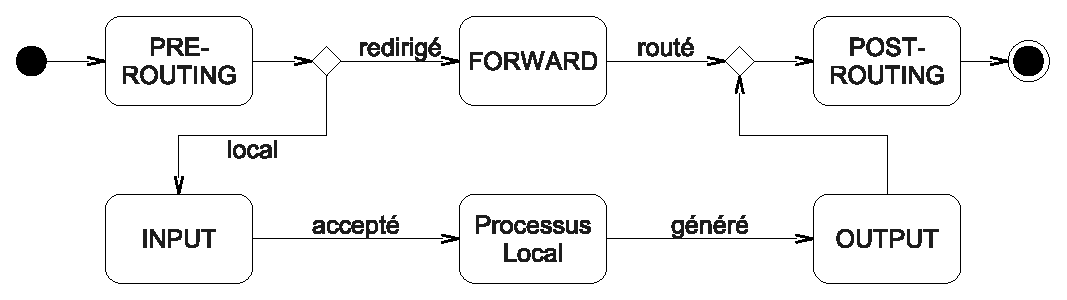
\includegraphics[width=\columnwidth]{firewall}
  \caption{Struktur des Paketfilters}
  \label{fig:netfilter}
\end{figure}

Mit der Paketfilterkonfiguration lassen sich die einzelnen
Ketten des Paketfilters direkt konfigurieren. Dazu gibt es für
jede relevante Kette ein eigenes Array, d.h. eine für die
\fwchain{INPUT}-Kette (\var{PF\_INPUT\_\%}), eine für die
\fwchain{FORWARD}-Kette (\var{PF\_FORWARD\_\%}), eine für die
\fwchain{OUTPUT}-Kette (\var{PF\_OUTPUT\_\%}), eine für die
\fwchain{PREROUTING}-Kette, in der die Portweiterleitung durchgeführt wird
(\var{PF\_PREROUTING\_\%}), und eine für die \fwchain{POSTROUTING}-Kette,
in der das Maskieren der Pakete durchgeführt wird (\var{PF\_POSTROUTING\_\%}).

Ein Eintrag in einem dieser Arrays besteht im
Wesentlichen aus einer Aktion (s.u.),
die durch zusätzliche Bedingungen eingeschränkt werden kann. Diese Bedingungen
beziehen sich auf Eigenschaften des betrachteten Paketes. Ein Paket
enthält Informationen über seine Herkunft (Quelle, welcher Rechner hat
das Paket losgeschickt), sein Ziel (an welchen Rechner und welche
Anwendung soll das Paket gehen) u.a.m. Bedingungen können sich auf
folgende Eigenschaften eines Paketes beziehen:

\begin{itemize}
  \item die Quelle (Quell-Adresse, Quell-Port oder beides)
  \item das Ziel (Ziel-Adresse, Ziel-Port oder beides)
  \item das Protokoll
  \item die Schnittstelle, über welches das Paket hereinkommt bzw. hinausgeht
  \item die MAC-Adresse des Rechners, von dem das Paket kommt
  \item den Zustand des Paketes bzw. der Verbindung, zu der das Paket gehört
\end{itemize}

Kommt ein Paket herein, werden die Einträge bzw. die daraus generierten
Regeln von oben nach unten abgearbeitet und die erste Aktion
ausgeführt, bei der alle Bedingungen gelten.  Trifft keine der Regeln
zu, wird die Standardaktion ausgeführt, die man für (fast) jede
Tabelle angeben kann.

Ein Eintrag hat dabei folgendes Format, wobei zu beachten ist, dass
alle Einschränkungen optional sind:

\begin{example}
\begin{verbatim}
    restriction{0,} [[source] [destination]] action [BIDIRECTIONAL|LOG|NOLOG]
\end{verbatim}
\end{example}

An allen Stellen, an denen Netzwerke, IP-Adressen oder Hosts angegeben werden
müssen, kann man sich auch auf \var{IP\_NET\_\%}, \var{IP\_NET\_\%\_IPADDR} oder
via \host{@hostname} auf einen Host aus \var{HOST\_\%} beziehen. Ist
\var{OPT\_DNS} aktiviert, dann können außerhalb von Aktionen via \host{@fqdn}
auch Hosts über ihren Namen referenziert werden, die \emph{nicht} in
\var{HOST\_\%} zu finden sind. Das ist insbesondere dann sinnvoll, wenn es
sich um externe Hosts handelt, die zudem viele (und wechselnde) IP-Adressen
besitzen.

\marklabel{sec:fwrules_actions}{\subsection{Aktionen des Paketfilters}}

Aktionen können die folgenden sein:
\begin{center}
    \begin{longtable}{|l|l|p{0.5\textwidth}|}
        \hline
        \multicolumn{1}{|l}{\textbf{Aktion}} &
        \multicolumn{1}{|l}{\textbf{Kette(n)}} &
        \multicolumn{1}{|l|}{\textbf{Bedeutung}} \\
        \hline
        \endhead
        \hline
        \endfoot
        \endlastfoot
        \fwaction{ACCEPT}       & alle
                                & Akzeptiere das Paket.
                                \\
        \hline
        \fwaction{DROP}         &
                                \begin{tabular}[t]{@{}l@{}}
                                    \fwchain{INPUT} \\
                                    \fwchain{FORWARD} \\
                                    \fwchain{OUTPUT}
                                \end{tabular}
                                & Verwirf das Paket (der Absender erkennt das
                                nur daran, dass keine Antwort, aber auch keine
                                Fehlermeldung zurückkommt).
                                \\
        \hline
        \fwaction{REJECT}       &
                                \begin{tabular}[t]{@{}l@{}}
                                    \fwchain{INPUT} \\
                                    \fwchain{FORWARD} \\
                                    \fwchain{OUTPUT}
                                \end{tabular}
                                & Weise das Paket zurück (der Absender erhält
                                eine entsprechende Fehlermeldung).
                                \\
        \hline
        \fwaction{LOG}          & alle
                                & Protokolliere das Paket und gehe zur nächsten
                                Regel. Um verschiedene Protokoll-Einträge
                                auseinanderhalten zu können, kann ein Präfix
                                verwendet werden, das via
                                \fwaction{LOG:log-prefix} angegeben wird. Dieses
                                Präfix darf maximal 28 Zeichen lang sein und
                                kann aus Buchstaben, Ziffern, dem Bindestrich
                                (\texttt{-}) und dem Unterstrich (\texttt{\_})
                                bestehen.
                                \\
        \hline
        \fwaction{MASQUERADE}   & \fwchain{POSTROUTING}
                                & Maskiere das Paket: Ersetze die Quelladresse
                                des Paketes durch die eigene, der Schnittstelle
                                zugewiesenen Adresse und sorge dafür, dass
                                Antworten für diese Verbindung an den richtigen
                                Rechner weitergeleitet werden.
                                \\
        \hline
        \fwaction{SNAT}         & \fwchain{POSTROUTING}
                                & Ersetze die Quelladresse und den Quellport
                                des Paketes durch die als Parameter für
                                \fwaction{SNAT} angegebene Adresse (für alle
                                Pakete, die zu der gerade betrachteten
                                Verbindung gehören).
                                \\
        \hline
        \fwaction{DNAT}         & \fwchain{PREROUTING}
                                & Ersetze die Zieladresse und den Zielport des
                                Paketes durch die als Parameter für
                                \fwaction{DNAT} angegebene Adresse (für alle
                                Pakete, die zu der gerade betrachteten
                                Verbindung gehören).
                                \\
        \hline
        \fwaction{REDIRECT}     &
                                \begin{tabular}[t]{@{}l@{}}
                                    \fwchain{PREROUTING} \\
                                    \fwchain{OUTPUT}
                                \end{tabular}
                                & Ersetze den Zielport des Paketes durch den
                                als Parameter für \fwaction{REDIRECT}
                                angegebenen Port und stelle das Paket lokal zu
                                (für alle Pakete, die zu der gerade
                                betrachteten Verbindung gehören).
                                \\
        \hline
        \fwaction{NETMAP}       &
                                \begin{tabular}[t]{@{}l@{}}
                                    \fwchain{PREROUTING} \\
                                    \fwchain{POSTROUTING}
                                \end{tabular}
                                & Bilde die Ziel- bzw. Quelladresse des Paketes
                                in den als Parameter für \fwaction{NETMAP}
                                angegebenen Bereich ab, die Ports bleiben
                                unverändert (für alle Pakete, die zu der gerade
                                betrachteten Verbindung gehören; in der
                                \fwchain{PREROUTING}-Kette wird die Zieladresse
                                verändert, in der \fwchain{POSTROUTING}-Kette
                                die Quelladresse).
                                \\
        \hline
        \caption{Aktionen in Paketfilterregeln}\marklabel{fwrule:actions}{}
    \end{longtable}
\end{center}

Einige dieser Aktionen können durch die Optionen \fwaction{BIDIRECTIONAL},
\fwaction{LOG} oder \fwaction{NOLOG} in ihrem Verhalten modifiziert werden.
\fwaction{BIDIRECTIONAL} generiert die gleiche Regel noch einmal, nur mit
vertauschter Quell- und Zieladresse (und vertauschtem Quell- und Zielport
und/oder vertauschter ein- und ausgehender Netzwerk-Schnittstelle, falls
angegeben). \fwaction{LOG}/\fwaction{NOLOG} aktivieren bzw. deaktivieren das
Protokollieren für diese eine Regel.

\marklabel{sec:fwrules_limits}{\subsection{Einschränkungen in den Regeln}}

Einschränkungen können durch die in den folgenden Abschnitten
aufgeführten Bedingungen vorgenommen werden. Bei den Bedingungen kann
man immer \fwmatch{any} angeben, wenn man an irgendeiner Stelle keine
Einschränkung vornehmen will, aber trotzdem etwas angeben
will/muss. Einschränkungen können in beliebiger Reihenfolge angegeben
werden, wenn sie einen vorangestellten Präfix haben. Das gilt für alle
Einschränkungen, außer für die Angabe einer Quell- bzw. Zieladresse. Diese
müssen immer direkt vor der Aktion stehen, die anderen Einschränkungen müssen
vorher erfolgen. Einschränkungen können auch negiert werden, dazu wird
einfach ein \fwmatch{!} vorangestellt.

\subsubsection{Einschränkungen der Quelle und des Ziels}

Jedes Paket enthält eine Quell- und eine Zielangabe, jeweils in Form
eines Tupels einer IP-Adresse und eines Ports.\footnote{Ein Port ist nur bei
TCP- und UDP-Paketen vorhanden.} Diese Quelle bzw. dieses Ziel kann für eine
Einschränkung herangezogen werden. Die Angabe für die Quelle bzw. das Ziel kann
folgendermaßen vorgenommen werden:

\begin{center}
    \begin{longtable}{|l|p{0.5\textwidth}|}
        \hline
        \multicolumn{1}{|l}{\textbf{Ausdruck}} &
        \multicolumn{1}{|l|}{\textbf{Bedeutung}} \\
        \hline
        \endhead
        \hline
        \endfoot
        \endlastfoot
    \verb+ip+               & eine einfache IP-Adresse\\
    \verb+network+          & eine Netzwerkangabe der Form \verb+<ip>/<netmask>+ \\
    \verb+port[-port]+      & ein Port bzw. ein Port-Bereich\\
    \verb+IP_NET_x_IPADDR+  & die IP-Adresse der Schnittstelle \verb+x+ des Routers\\
    \verb+IP_NET_x+         & das Subnetz \verb+x+ des Routers\\
    \verb+IP_ROUTE_x+       & das in der Route \verb+x+ angegebene Subnetz
      (Default-Routen können nicht verwendet werden, sie würden \fwmatch{any} entsprechen und
      werden vorsichtshalber ausgeklammert)\\
    \verb+@name+            & einer der via HOST\_\%\_* vergebenen Namen oder
      Aliase; es wird die zugehörige IP-Adresse an dieser Stelle eingesetzt\\
    \verb+<ip oder netzwerk>:port[-port]+ & Host- bzw. Netzwerk-Adresse in einer
      der obigen Varianten, kombiniert mit einem Port bzw. Port-Bereich\\
        \hline
        \caption{Quell- und Zieleinschränkungen in Paketfilterregeln}
    \end{longtable}
\end{center}

\noindent Das könnte z.\,B. wie folgt aussehen: \verb+'192.168.6.2 any DROP'+

Tauchen zwei dieser Angaben auf, wird die erste als Quelle, die zweite
als Ziel betrachtet. In diesem Beispiel verwerfen wir also Pakete, die
vom Rechner mit der IP-Adresse 192.168.6.2 gesendet wurden, unabhängig
davon, an welches Ziel sie gerichtet sind.

Taucht nur eine Angabe auf, wird anhand des Wertes entschieden, ob die
Quelle oder das Ziel gemeint ist, wobei die Entscheidung relativ
einfach ist:
\begin{itemize}
  \item Ist eine Port-Angabe enthalten, ist das Ziel gemeint.
  \item Sonst ist die Quelle gemeint.
\end{itemize}

Wenn wir also z.\,B. das obige Beispiel abkürzen wollten,
könnten wir einfach \verb+'192.168.6.2 DROP'+ schreiben. Es ist kein
Port angegeben, die Bedingung gilt also für die Quelle, den Rechner,
von dem das Paket gesendet wurde.

Wollen wir die Kommunikation mit dem \protocol{ssh}-Dämon erlauben, können
wir \verb+'any any:22 ACCEPT'+ (Pakete von einem beliebigen Rechner an den
\protocol{ssh}-Port 22 eines beliebigen Rechners werden akzeptiert) oder
kürzer \verb+'22 ACCEPT'+ schreiben: Es ist nur ein Port angegeben,
also meinen wir das Ziel und damit Pakete, die an den Port 22
gerichtet sind.

Zur Vereinfachung der Regelmenge kann man an die Aktion ein
\fwaction{BIDIRECTIONAL} dranhängen, um auszudrücken, dass die Regel für beide
Kommunikationsrichtungen gilt. Es werden dann Regeln generiert, in
denen einfach die Quell- und die Ziel-Adressen und eventuell angegebenene Ports
und Netzwerk-Schnittstellen vertauscht sind und der Rest gleich bleibt.

Beispiele:
\medskip

\begin{example}
\noindent
{\footnotesize
 \begin{tabular}{@{}p{5cm}p{10cm}@{}}
    \verb+127.0.0.1 ACCEPT+             & Lokale Kommunikation (Quelle 127.0.0.1) ist erlaubt \\
    \verb+any 192.168.12.1 DROP+        & Pakete an die Adresse 192.168.12.1 werden weggeworfen \\
    \verb+any 192.168.12.1 DROP LOG+    & Pakete an die Adresse 192.168.12.1 werden weggeworfen und zusätzlich protokolliert \\
    \verb+any 192.168.12.1 DROP NOLOG+  & Pakete an die Adresse 192.168.12.1 werden weggeworfen, werden aber nicht protokolliert \\
    \verb+22 ACCEPT+                    & Pakete an den Port 22 (\protocol{ssh}) werden akzeptiert \\
    \verb+IP_NET_1_NET ACCEPT+          & Pakete aus dem an der ersten Schnittstelle hängenden Subnetz werden akzeptiert\\
    \verb+IP_NET_1_NET IP_NET_2_NET+    & Kommunikation zwischen den an der ersten und zweiten\\
    \verb+  ACCEPT BIDIRECTIONAL+       & Schnittstelle hängenden Subnetzen ist gestattet
 \end{tabular}
}
\end{example}

\subsubsection{Einschränkung der Schnittstelle}

Eine Regel kann eingeschränkt werden in Bezug auf die Schnittstelle, über die
ein Paket hereinkam bzw. hinausgeht. Das Format sieht wie folgt aus:
\fwmatch{if:}\emph{in}\fwmatch{:}\emph{out}

In der \fwchain{INPUT}-Kette kann man die Schnittstelle für hinausgehende
Pakete nicht einschränken (das Paket geht ja nicht mehr hinaus), in der
\fwchain{POSTROUTING}-Kette kann man die Schnittstelle für hereinkommende
Pakete nicht einschränken, da die Information darüber nicht mehr vorhanden ist.
Lediglich in der \fwchain{FORWARD}-Kette kann man für beides Bedingungen
angeben.

Möglich sind folgende Werte für \emph{in} bzw. \emph{out}:

\begin{itemize}
  \item \fwmatch{lo} (Loopback-Schnittstelle, lokale Kommunikation auf dem
    Router)
  \item \verb+IP_NET_x_DEV+
  \item \fwmatch{pppoe} (die PPPoE-Schnittstelle; nur bei entsprechend
    aktiviertem \package{dsl}- oder \package{pppoe\_server}-Paket)
  \item \fwmatch{any}
\end{itemize}

\subsubsection{Einschränkungen des Protokolls}

Eine Regel kann eingeschränkt werden in Bezug auf das Protokoll, zu dem ein
Paket gehört. Das Format sieht wie folgt aus:
\fwmatch{prot:}\emph{protocol} bzw. \fwmatch{prot:}\emph{icmp}\fwmatch{:}\emph{icmp-type}.
\emph{protocol} kann dabei einen der folgenden Werte annehmen:

\begin{itemize}
  \item \fwmatch{tcp}
  \item \fwmatch{udp}
  \item \fwmatch{gre} (Generic Routing Encapsulation)
  \item \fwmatch{icmp} (hier kann man zusätzlich noch einen Namen für den
    zu filternden ICMP-Typ angeben (\fwmatch{echo-reply} oder
    \fwmatch{echo-request}), etwa \fwmatch{prot:icmp:echo-request})
  \item numerischer Wert der Protokoll-ID (z.\,B. 41 für IPv6)
  \item \fwmatch{any}
\end{itemize}

Wenn eine solche Einschränkung nicht vorhanden ist, aber dennoch Portnummern
in einer Regel verwendet werden, dann wird die Regel \emph{zweimal} angelegt,
nämlich einmal für das \protocol{tcp}- und einmal für das
\protocol{udp}-Protokoll.

\subsubsection{Einschränkung der MAC-Adresse}

Mittels \fwmatch{mac:}\emph{mac-address} kann eine Einschränkung bezüglich der
MAC-Adresse vorgenommen werden.

\subsubsection{Einschränkungen in Bezug auf den Zustand eines Paketes}

Der von fli4l verwendete Paketfilter sammelt Informationen über den
Zustand von Verbindungen. Diese Informationen kann man dann nutzen, um
Pakete zu filtern, also z.\,B. nur Pakete durchzulassen, die zu bereits
bestehenden Verbindungen gehören. Die Zustände einer Verbindung können
sein:\footnote{siehe \altlink{http://www.sns.ias.edu/~jns/files/iptables_talk/x38.htm}
für eine genauere Beschreibung der Zustände}

\begin{center}
    \begin{longtable}{|l|p{0.7\textwidth}|}
        \hline
        \multicolumn{1}{|l}{\textbf{Zustand}} &
        \multicolumn{1}{|l|}{\textbf{Bedeutung}} \\
        \hline
        \endhead
        \hline
        \endfoot
        \endlastfoot
        \fwpktstate{INVALID}        & Das Paket gehört zu keiner bekannten
                                    Verbindung.
                                    \\
        \fwpktstate{ESTABLISHED}    & Das Paket gehört zu einer Verbindung,
                                    über die bereits in beide Richtungen Pakete
                                    geflossen sind.
                                    \\
        \fwpktstate{NEW}            & Das Paket hat eine neue Verbindung
                                    aufgebaut oder gehört zu einer Verbindung,
                                    bei der noch nicht Pakete in beide
                                    Richtungen geflossen sind.
                                    \\
        \fwpktstate{RELATED}        & Das Paket baut eine neue Verbindung auf,
                                    hat aber eine Beziehung zu einer
                                    bestehenden Verbindung (z.\,B. baut
                                    \protocol{ftp} eine separate Verbindung für
                                    den eigentlichen Datentransfer auf).
                                    \\
        \hline
        \caption{Zustandseinschränkungen in Paketfilterregeln}
    \end{longtable}
\end{center}

Die Zustände werden wie folgt angegeben:
\fwmatch{state:}\emph{state(s)}. Will man mehrere
Zustände angeben, werden diese mit Komma getrennt. Um z.\,B. nur Pakete
durchzulassen, die direkt oder indirekt zu bestehenden Verbindungen gehören,
kann man \fwmatch{state:}\fwpktstate{ESTABLISHED,RELATED} schreiben (dies ist
in der \fwchain{INPUT}- oder \fwchain{FORWARD}-Kette sinnvoll).

\subsubsection{Einschränkung der Häufigkeit einer Aktion}

Unter bestimmten Umständen möchte man die Häufigkeit von Aktionen
begrenzen, z.\,B. nur eine ICMP-Echo-Anforderung pro Sekunde zulassen. Das
kann man mit der \fwmatch{limit}-Einschränkung erreichen, die wie folgt
aussieht: \fwmatch{limit:}\emph{Häufigkeit:Burst}. Die
Häufigkeit wird dabei als \emph{n/Zeiteinheit} (second, minute, hour, day)
angegeben, wobei zusätzlich noch Ereignisse gehäuft auftreten
können (Burst). Die Angabe \texttt{limit:3/minute:5} heißt z.\,B., dass
höchstens drei Ereignisse pro Minute erlaubt sind, wobei auch mal fünf
Ereignisse dicht aufeinander folgend akzeptiert werden.

\marklabel{sec:templates}{\subsection{Der Einsatz von Schablonen im Paketfilter}}

Um den Umgang mit dem Paketfilter weiter zu vereinfachen, gibt es die
Möglichkeit, häufig vorkommende Regeln zu sogenannten Schablonen (Templates)
zusammenzufassen. Damit ist es möglich, eine ganze Reihe von
Paketfilterregeln zusammenzufassen und dieser Sammlung von Regeln
einen symbolischen Namen zu geben. Anstatt direkt mit Protokollen und
Portnummern zu hantieren, verwenden Sie dann Einträge wie \fwmatch{tmpl:ssh},
wenn Sie das \protocol{ssh}-Protokoll in einer Regel verwenden wollen. Wie mit
Schablonen zu verfahren ist, wird hier am Beispiel von \protocol{ssh} gezeigt.

Wollen Sie Ihren fli4l-Router vom Internet aus per \protocol{ssh} erreichen, so
schreiben Sie in einen Eintrag der Array-Variable \var{PF\_INPUT\_\%} den
entsprechenden Dienstnamen (hier \protocol{ssh}) mit vorangestelltem
\fwmatch{tmpl:} und der Aktion, die für diesen Dienst gelten soll. Beispiel:

\begin{example}
\begin{verbatim}
    PF_INPUT_2='tmpl:ssh ACCEPT'
\end{verbatim}
\end{example}

Hierbei steht \fwmatch{tmpl:} dafür, dass eine Regel auf einer Schablone
basieren soll. Den Namen des Dienstes geben Sie nach dem `:'
an, in unserem Beispiel also \protocol{ssh}. Zum Schluss geben Sie an, welche
Aktion mit dem Dienst verbunden werden soll. Da Sie den fli4l-Router
aus dem Internet erreichen wollen, erlauben wir die Verbindung mit
\fwaction{ACCEPT}. Einschränkungen von IP-Adressen oder Netzen sind nicht
angegeben, also ist der \protocol{ssh}-Dienst von allen Netzen und über alle
Schnittstellen erreichbar. Sie könnten bei Bedarf die gewohnten Schreibweisen
vom Paketfilter benutzen, um den Zugriff auf den \protocol{ssh}-Dienst weiter
einzuschränken.

Für welche Dienste Regeln vorbereitet sind (d.h. Schablonen existieren),
kann in der Schablonen-Datei in \verb+opt/etc/fwrules.tmpl/templates+
nachgelesen werden. Im Folgenden finden Sie die Aufstellung in Tabellenform
(siehe Tabelle \ref{tab:fwrules_tmpl}).

\begin{center}
  {\footnotesize
  \begin{longtable}{|lll|}
     \hline
     {\textbf{Schablone}} & {\textbf{Protokoll}} & {\textbf{Port(s)}} \\
     \hline\hline
     \endhead
     \input{fwrules_tmpl_table.inc} \\
     \caption{Im Lieferumfang von fli4l enthaltene Schablonen}
     \label{tab:fwrules_tmpl}
  \end{longtable}}
\end{center}

Die Syntax für diese Form der Paketfilterregeln lautet also immer

\begin{example}
\begin{verbatim}
    tmpl:<Name des Dienstes> <Einschränkungen> <Gewünschte Aktion>
\end{verbatim}
\end{example}

wobei als \verb+<Einschränkungen>+ alles erlaubt ist, was unter
\ref{sec:fwrules_limits} beschrieben wird. Die möglichen Werte für
\verb+<Gewünschte Aktion>+ sind in \ref{sec:fwrules_actions} aufgelistet und
beschrieben.

Ein paar weitere Beispiele sollen die Arbeitsweise verdeutlichen. Zuerst
wollen wir uns \var{PF\_PREROUTING} ansehen:

\begin{example}
\begin{verbatim}
    PF_PREROUTING_N='2'
    PF_PREROUTING_1='tmpl:xbl dynamic DNAT:@xbox'
    PF_PREROUTING_2='tmpl:https dynamic DNAT:192.168.193.250'
\end{verbatim}
\end{example}

Die Regel \var{PF\_PREROUTING\_1} versorgt die Xbox mit allem, was für
Xbox Live notwendig ist. Im einzelnen werden mit \fwmatch{tmpl:xbl} alle Ports
und Protokolle, die für Xbox Live notwendig sind, an den Host \host{xbox}
weitergeleitet. Anstelle der IP-Adresse wird ein Eintrag aus dem
\var{HOST\_\%\_NAME}-Array benutzt. Durch \fwmatch{dynamic} weiß der fli4l,
dass die Ports von der Internet-Schnittstelle weitergeleitet werden sollen.

Die zweite Regel leitet das \protocol{https}-Protokoll an einen Webserver in
der DMZ weiter.

Jetzt sehen wir uns an, wie es mit \var{PF\_INPUT} weitergeht:

\begin{example}
\begin{verbatim}
    PF_INPUT_N='3'
    PF_INPUT_1='if:IP_NET_1_DEV:any ACCEPT'
    PF_INPUT_2='if:pppoe:any prot:tcp 113 ACCEPT'
    PF_INPUT_3='if:br0:any tmpl:dns @xbox IP_NET_1_IPADDR ACCEPT'
\end{verbatim}
\end{example}

Die erste Regel lässt alle aus dem Netz, das mit \var{IP\_NET\_1} definiert
ist, auf den Router zugreifen. Die zweite Regel ist für das
\package{oident}-Paket. Dort wird der \protocol{ident}-Port geöffnet. Die
dritte und letzte Regel erlaubt der Xbox den Zugriff auf den DNS Server auf dem
fli4l. Hier ist auch wieder schön zu sehen, wie man einen Host-Alias einsetzt.

In \var{PF\_FORWARD} und \var{PF\_POSTROUTING} steht nichts
\fwmatch{tmpl}-spezifisches mehr.

\begin{figure}[htbp]
  \centering
  \includegraphics[width=0.9\columnwidth]{etc_fwrules_tmpl_dir}
  \caption{Verzeichnisstruktur fli4l}
  \label{fig:etc_fwrules_tmpl_dir}
\end{figure}

Es ist auch möglich, dass Sie eigene Schablonen anlegen oder dass
Pakete ihre eigenen Schablonen mitbringen. Um eine eigene
Schablone anzulegen, muss lediglich eine Datei mit den Namen der
Schablone erstellt und die entsprechenden Regeln dort
aufgenommen werden. Wenn Sie eine private Schablonendatei anlegen wollen,
erstellen Sie diese in dem Verzeichnis \verb+etc/fwrules.tmpl+ unterhalb Ihres
\texttt{config}-Verzeichnisses, so wie es die Abbildung
\ref{fig:etc_fwrules_tmpl_dir} zeigt. Wenn das Verzeichnis
\texttt{etc/fwrules.tmpl} unterhalb Ihres \texttt{config}-Verzeichnisses noch
nicht existiert, legen Sie bitte zuerst beide Verzeichnisse an. Alternativ
können Paket-Entwickler oder Benutzer, die Schablonen für mehr als eine
Konfiguration anlegen wollen, ihre Regeln direkt in das Verzeichnis
\texttt{opt/etc/fwrules.tmpl} ablegen. In dieses Verzeichnis kommen dann die
neuen Schablonen. Dabei gilt die Regel, dass die Schablonen im
\texttt{config}-Verzeichnis des Benutzers vorrangig behandelt werden.
Zum Schluss wird die Schablonendatei, die zum Lieferumfang von
fli4l gehört, ausgewertet. Sie können also Einträge in der fli4l-Schablonendatei
dadurch \glqq{}überschreiben\grqq{}, indem Sie eine
Schablonendatei mit dem Namen der zu überschreibenden Schablone in Ihrem
\texttt{config}-Verzeichnis anlegen.

Wenn Sie zum Beispiel die Schablone \fwmatch{vpn\_freunde} anlegen wollen, legen
Sie die Datei \texttt{vpn\_freunde} an. Das Template soll die Dienste
\protocol{ssh}, \protocol{smtp}, \protocol{dns} und \protocol{samba} enthalten.
Also schreiben Sie in die Datei \texttt{vpn\_freunde} Folgendes:

\begin{example}
\begin{verbatim}
    prot:tcp 22
    prot:tcp 25
    53
    prot:udp 137-138
    prot:tcp 139
    prot:tcp 445
\end{verbatim}
\end{example}

\noindent Wann immer Sie jetzt die Schablone \fwmatch{vpn\_freunde} benutzen,
werden daraus Regeln für alle darin aufgeführten Protokolle und Ports erzeugt.
\verb+PF_FORWARD_x='tmpl:vpn_freunde ACCEPT'+ etwa erstellt folgende
\fwchain{FORWARD}-Regeln:

\begin{example}
\begin{verbatim}
    prot:tcp 22 ACCEPT
    prot:tcp 25 ACCEPT
    53 ACCEPT
    prot:udp 137-138 ACCEPT
    prot:tcp 139 ACCEPT
    prot:tcp 445 ACCEPT
\end{verbatim}
\end{example}

\subsection{Die Konfiguration des Paketfilters}

Der Paketfilter wird im Wesentlichen durch vier Array-Variablen konfiguriert:

\begin{itemize}
  \item \var{PF\_INPUT\_\%} konfiguriert die \fwchain{INPUT}-Kette,
  \item \var{PF\_FORWARD\_\%} konfiguriert die \fwchain{FORWARD}-Kette,
  \item \var{PF\_OUTPUT\_\%} konfiguriert die \fwchain{OUTPUT}-Kette,
  \item \var{PF\_PREROUTING\_\%} konfiguriert die \fwchain{PREROUTING}-Kette und
  \item \var{PF\_POSTROUTING\_\%} konfiguriert die \fwchain{POSTROUTING}-Kette.
\end{itemize}

\configlabel{PF\_LOG\_LEVEL}{PFLOGLEVEL} Für alle folgenden Ketten
gilt die in \var{PF\_LOG\_LEVEL} vorgenommene Einstellung der
Protokoll-Stufe, deren Inhalt auf einen der folgenden Werte gesetzt werden
kann: \fwloglevel{debug}, \fwloglevel{info}, \fwloglevel{notice},
\fwloglevel{warning}, \fwloglevel{err}, \fwloglevel{crit}, \fwloglevel{alert},
\fwloglevel{emerg}.

\subsubsection{Die \fwchain{INPUT}-Kette}

Über die \fwchain{INPUT}-Kette wird konfiguriert, wer auf den Router zugreifen
darf. Trifft keine der Regeln der \fwchain{INPUT}-Kette zu, bestimmt die
Standard-Aktion, was mit dem Paket passieren soll, und die Protokoll-Variable
bestimmt, ob es bei einer Ablehnung ins System-Protokoll geschrieben werden soll.

Bei den verwendeten Parametern gibt es die folgenden Einschränkungen:
\begin{itemize}
  \item Es können nur \fwaction{ACCEPT}, \fwaction{DROP} und \fwaction{REJECT}
    als Aktion angegeben werden.
  \item Bei einer Schnittstellen-Einschränkung kann man nur die
    Eingangsschnittstelle einschränken.
\end{itemize}

\begin{description}
\config{PF\_INPUT\_POLICY}{PF\_INPUT\_POLICY}{PFINPUTPOLICY}
Diese Variable beschreibt die Standard-Aktion, die angewandt wird,
wenn keine der anderen Regeln zutrifft. Möglich sind:

\begin{itemize}
\item \fwaction{ACCEPT} (nicht empfohlen)
\item \fwaction{REJECT}
\item \fwaction{DROP} (nicht empfohlen)
\end{itemize}

\config{PF\_INPUT\_ACCEPT\_DEF}{PF\_INPUT\_ACCEPT\_DEF}{PFINPUTACCEPTDEF}
Steht diese Variable auf `yes', werden Standard-Regeln generiert, die
für ein korrektes Funktionieren des Routers notwendig
sind. Standardmäßig sollte man hier `yes' eintragen.

Möchte man das Verhalten komplett selbst definieren, kann man
hier `no' eintragen, muss dann jedoch alle Regeln selbst definieren.
Eine zum Standardverhalten äquivalente Konfiguration würde wie folgt
aussehen (die Beschreibung der Liste für benutzerdefinierte Ketten erfolgt
\jump{sec:userlists}{hier}):

\begin{example}
{\footnotesize
\begin{verbatim}
    PF_INPUT_ACCEPT_DEF='no'
    #
    # limit ICMP echo requests - use a separate chain
    #
    PF_USR_CHAIN_N='1'
    PF_USR_CHAIN_1_NAME='usr-in-icmp'
    PF_USR_CHAIN_1_RULE_N='2'
    PF_USR_CHAIN_1_RULE_1='prot:icmp:echo-request length:0-150 limit:1/second:5 ACCEPT'
    PF_USR_CHAIN_1_RULE_2='state:RELATED ACCEPT'

    PF_INPUT_N='4'
    PF_INPUT_1='prot:icmp usr-in-icmp'
    PF_INPUT_2='state:ESTABLISHED,RELATED ACCEPT'
    PF_INPUT_3='if:lo:any ACCEPT'
    PF_INPUT_4='state:NEW 127.0.0.1 DROP BIDIRECTIONAL'
\end{verbatim}}
\end{example}

Die erste Regel verzweigt zur ratenlimitierenden ``usr-in-icmp''-Kette.
Die zweite Regel akzeptiert nur solche Pakete, die zu bestehenden Verbindungen
gehören (also Paketen, die entweder den Zustand \fwpktstate{ESTABLISHED} oder
\fwpktstate{RELATED} besitzen), und die dritte erlaubt lokale Kommunikation
(\verb+if:lo:any ACCEPT+). Die vierte filtert Pakete heraus,
die behaupten, lokale Kommunikation zu sein, aber nicht bereits von
der vorherigen Regel akzeptiert wurden.

Arbeitet man mit OpenVPN, muss man die Regeln
noch ergänzen, um die von diesen Paketen verwendeteten Ketten
einzubinden.

\begin{example}
\begin{verbatim}
    PF_INPUT_N='5'
    ...
    PF_INPUT_5='ovpn-chain'
\end{verbatim}
\end{example}

\config{PF\_INPUT\_LOG}{PF\_INPUT\_LOG}{PFINPUTLOG}
Definiert, ob abgelehnte Pakete vom Kernel protokolliert werden sollen.
Dabei können die Meldungen durch Aktivierung von \var{OPT\_KLOGD} über den
syslog-Dämon entsprechend der Konfiguration ausgegeben werden.

\config{PF\_INPUT\_LOG\_LIMIT}{PF\_INPUT\_LOG\_LIMIT}{PFINPUTLOGLIMIT}
Definiert, wie häufig Log-Einträge generiert werden. Die Häufigkeit
wird analog zur Limit-Einschränkung als \emph{n/Zeiteinheit} mit Bursts
beschrieben, also z.\,B. \texttt{3/minute:5}. Ist dieser Eintrag leer, wird der
Standardwert \texttt{1/second:5} verwendet; enhält er \texttt{none}, wird keine
Limitierung durchgeführt.

\configlabel{PF\_INPUT\_UDP\_REJ\_LIMIT}{PFINPUTUDPREJLIMIT}
\config{PF\_INPUT\_REJ\_LIMIT PF\_INPUT\_UDP\_REJ\_LIMIT}{PF\_INPUT\_REJ\_LIMIT}{PFINPUTREJLIMIT}
Definiert, wie häufig bei einer Ablehnung eines hereinkommenden Paketes
auch ein entsprechendes \fwaction{REJECT}-Paket generiert wird. Die Häufigkeit
wird analog zur Limit-Einschränkung als \emph{n/Zeiteinheit} mit Bursts
beschrieben, also z.\,B. \texttt{3/minute:5}. Ist das Limit überschritten, wird
das Paket einfach ignoriert (\fwaction{DROP}). Ist dieser Eintrag leer, wird
der Standardwert \texttt{1/second:5} verwendet; enhält er \texttt{none}, wird
keine Limitierung durchgeführt.

\config{PF\_INPUT\_ICMP\_ECHO\_REQ\_LIMIT}{PF\_INPUT\_ICMP\_ECHO\_REQ\_LIMIT}{PFINPUTICMPECHOREQLIMIT}
Definiert, wie häufig auf eine ICMP-Echo-Anfrage reagiert werden soll.
Die Häufigkeit wird analog zur Limit-Einschränkung als \emph{n/Zeitein-heit}
mit Bursts beschrieben, also z.\,B. \texttt{/minute:5}. Ist das
Limit überschritten, wird das Paket einfach ignoriert (\fwaction{DROP}). Ist
dieser Eintrag leer, wird der Standardwert \texttt{1/second:5} verwendet;
enhält er \texttt{none}, wird keine Limitierung durchgeführt.

\config{PF\_INPUT\_ICMP\_ECHO\_REQ\_SIZE}{PF\_INPUT\_ICMP\_ECHO\_REQ\_SIZE}{PFINPUTICMPECHOREQSIZE}
Definiert, wie groß eine empfangene ICMP-Echo-Anfrage sein darf (in Bytes). In
dieser Angabe sind neben den ``Nutzdaten'' auch die Paket-Header mit zu
berücksichtigen. Der Standard-Wert liegt bei 150 Bytes.

\configlabel{PF\_INPUT\_x}{PFINPUTx}
\configlabel{PF\_INPUT\_x\_COMMENT}{PFINPUTxCOMMENT}
\config{PF\_INPUT\_N PF\_INPUT\_x PF\_INPUT\_x\_COMMENT}{PF\_INPUT\_N}{PFINPUTN}
Liste der Regeln, die beschreiben, welche Pakete vom Router angenommen
bzw. verworfen werden.
\end{description}

\subsubsection{Die \fwchain{FORWARD}-Kette}

Über die \fwchain{FORWARD}-Kette wird konfiguriert, welche Pakete vom Router
weitergeleitet werden. Trifft keine der Regeln der \fwchain{FORWARD}-Kette zu,
bestimmt die Standard-Aktion, was mit dem Paket passieren soll,und die
Protokoll-Variable bestimmt, ob es bei einer Ablehnung ins System-Protokoll
geschrieben werden soll.

Bei den verwendeten Parametern gibt es die Einschränkung, dass nur
\fwaction{ACCEPT}, \fwaction{DROP} und \fwaction{REJECT} als Aktion angegeben
werden können.

\begin{description}
\config{PF\_FORWARD\_POLICY}{PF\_FORWARD\_POLICY}{PFFORWARDPOLICY}
Diese Variable beschreibt die Standard-Aktion, die angewandt wird,
wenn keine der anderen Regeln zutrifft. Möglich sind:

\begin{itemize}
\item \fwaction{ACCEPT}
\item \fwaction{REJECT}
\item \fwaction{DROP}
\end{itemize}

\config{PF\_FORWARD\_ACCEPT\_DEF}{PF\_FORWARD\_ACCEPT\_DEF}{PFFORWARDACCEPTDEF}
Bestimmt, ob der Router Pakete akzeptiert, die zu bestehenden
Verbindungen gehören. Steht diese Variable auf `yes', generiert fli4l
automatisch eine Regel, die Pakete mit dem entsprechenden Zustand
akzeptiert:

\verb+'state:ESTABLISHED,RELATED ACCEPT'+,

weiterhin eine Regel, die Pakete mit unbekanntem Zustand verwirft:

\verb+'state:INVALID DROP'+.

und schließlich eine Regel, die Pakete mit gefälschten IP-Adressen verwirft:

\verb+'state:NEW 127.0.0.1 DROP BIDIRECTIONAL'+.

Zusätzlich generieren die
anderen Subsysteme auch noch Standardregeln~-- eine Konfiguration ohne
Standardregeln mit Portweiterleitung und OpenVPN würde mindestens
folgende Regeln enthalten:

\begin{example}
\begin{verbatim}
    PF_FORWARD_ACCEPT_DEF='no'
    PF_FORWARD_N='5'
    PF_FORWARD_1='state:ESTABLISHED,RELATED ACCEPT'
    PF_FORWARD_2='state:INVALID DROP'
    PF_FORWARD_3='state:NEW 127.0.0.1 DROP BIDIRECTIONAL'
    PF_FORWARD_4='pfwaccess-chain'
    PF_FORWARD_5='ovpn-chain'
\end{verbatim}
\end{example}

\config{PF\_FORWARD\_LOG}{PF\_FORWARD\_LOG}{PFFORWARDLOG}
Definiert, ob abgelehnte Pakete vom Kernel protokolliert werden sollen.
Dabei können die Meldungen durch Aktivierung von \var{OPT\_KLOGD} über den
syslog-Dämon entsprechend der Konfiguration ausgegeben werden.

\config{PF\_FORWARD\_LOG\_LIMIT}{PF\_FORWARD\_LOG\_LIMIT}{PFFORWARDLOGLIMIT}
Definiert, wie häufig Log-Einträge generiert werden. Die Häufigkeit
wird analog zur Limit-Einschränkung als \emph{n/Zeiteinheit} mit Bursts
beschrieben, also z.\,B. \texttt{3/minute:5}. Ist dieser Eintrag leer, wird der
Standardwert \texttt{1/second:5} verwendet; enhält er \texttt{none}, wird keine
Limitierung durchgeführt.

\configlabel{PF\_FORWARD\_UDP\_REJ\_LIMIT}{PFFORWARDUDPREJLIMIT}
\config{PF\_FORWARD\_REJ\_LIMIT PF\_FORWARD\_UDP\_REJ\_LIMIT}{PF\_FORWARD\_REJ\_LIMIT}{PFFORWARDREJLIMIT}
Definiert, wie häufig bei einer Ablehnung eines hereinkommenden Paketes
auch ein entsprechendes \fwaction{REJECT}-Paket generiert wird. Die Häufigkeit
wird analog zur Limit-Einschränkung als \emph{n/Zeiteinheit} mit Bursts
beschrieben, also z.\,B. \texttt{3/minute:5}. Ist das Limit überschritten, wird
das Paket einfach ignoriert (\fwaction{DROP}). Ist dieser Eintrag leer, wird
der Standardwert \texttt{1/second:5} verwendet; enhält er \texttt{none}, wird
keine Limitierung durchgeführt.

\configlabel{PF\_FORWARD\_x}{PFFORWARDx}
\configlabel{PF\_FORWARD\_x\_COMMENT}{PFFORWARDxCOMMENT}
\config{PF\_FORWARD\_N PF\_FORWARD\_x PF\_FORWARD\_x\_COMMENT}{PF\_FORWARD\_N}{PFFORWARDN}
Liste der Regeln, die beschreiben, welche Pakete vom Router
weitergeleitet bzw. verworfen werden.
\end{description}

\subsubsection{Die \fwchain{OUTPUT}-Kette}

Über die \fwchain{OUTPUT}-Kette wird konfiguriert, worauf der Router selbst
zugreifen darf. Trifft keine der Regeln der \fwchain{OUTPUT}-Kette zu, bestimmt
die Standard-Aktion, was mit dem Paket passieren soll, und die
Protokoll-Variable bestimmt, ob es bei einer Ablehnung ins System-Protokoll
geschrieben werden soll.

Bei den verwendeten Parametern gibt es die folgenden Einschränkungen:
\begin{itemize}
  \item Es können nur \fwaction{ACCEPT}, \fwaction{DROP} und \fwaction{REJECT}
    als Aktion angegeben werden.
  \item Bei einer Schnittstellen-Einschränkung kann man nur die
    Ausgangsschnittstelle einschränken.
\end{itemize}

\begin{description}
\config{PF\_OUTPUT\_POLICY}{PF\_OUTPUT\_POLICY}{PFOUTPUTPOLICY}
Diese Variable beschreibt die Standard-Aktion, die angewandt wird,
wenn keine der anderen Regeln zutrifft. Möglich sind:

\begin{itemize}
\item \fwaction{ACCEPT}
\item \fwaction{REJECT}
\item \fwaction{DROP}
\end{itemize}

\config{PF\_OUTPUT\_ACCEPT\_DEF}{PF\_OUTPUT\_ACCEPT\_DEF}{PFOUTPUTACCEPTDEF}
Steht diese Variable auf `yes', werden Standard-Regeln generiert, die
für ein korrektes Funktionieren des Routers notwendig
sind. Standardmäßig sollte man hier `yes' eintragen.

Möchte man das Verhalten komplett selbst definieren, kann man
hier `no' eintragen, muss dann jedoch alle Regeln selbst definieren.
Eine zum Standardverhalten äquivalente Konfiguration würde wie folgt
aussehen:

\begin{example}
{\footnotesize
\begin{verbatim}
    PF_OUTPUT_ACCEPT_DEF='no'

    PF_OUTPUT_N='1'
    PF_OUTPUT_1='state:ESTABLISHED,RELATED ACCEPT'
\end{verbatim}}
\end{example}

Die erste (und einzige) Regel akzeptiert nur solche Pakete, die zu bestehenden
Verbindungen gehören (also Paketen, die entweder den Zustand
\fwpktstate{ESTABLISHED} oder \fwpktstate{RELATED} besitzen).

\config{PF\_OUTPUT\_LOG}{PF\_OUTPUT\_LOG}{PFOUTPUTLOG}
Definiert, ob abgelehnte Pakete vom Kernel protokolliert werden sollen.
Dabei können die Meldungen durch Aktivierung von \var{OPT\_KLOGD} über den
syslog-Dämon entsprechend der Konfiguration ausgegeben werden.

\config{PF\_OUTPUT\_LOG\_LIMIT}{PF\_OUTPUT\_LOG\_LIMIT}{PFOUTPUTLOGLIMIT}
Definiert, wie häufig Log-Einträge generiert werden. Die Häufigkeit
wird analog zur Limit-Einschränkung als \emph{n/Zeiteinheit} mit Bursts
beschrieben, also z.\,B. \texttt{3/minute:5}. Ist dieser Eintrag leer, wird der
Standardwert \texttt{1/second:5} verwendet; enhält er \texttt{none}, wird keine
Limitierung durchgeführt.

\configlabel{PF\_OUTPUT\_UDP\_REJ\_LIMIT}{PFOUTPUTUDPREJLIMIT}
\config{PF\_OUTPUT\_REJ\_LIMIT PF\_OUTPUT\_UDP\_REJ\_LIMIT}{PF\_OUTPUT\_REJ\_LIMIT}{PFOUTPUTREJLIMIT}
Definiert, wie häufig bei einer Ablehnung eines hereinkommenden Paketes
auch ein entsprechendes \fwaction{REJECT}-Paket generiert wird. Die Häufigkeit
wird analog zur Limit-Einschränkung als \emph{n/Zeiteinheit} mit Bursts
beschrieben, also z.\,B. \texttt{3/minute:5}. Ist das Limit überschritten, wird
das Paket einfach ignoriert (\fwaction{DROP}). Ist dieser Eintrag leer, wird
der Standardwert \texttt{1/second:5} verwendet; enhält er \texttt{none}, wird
keine Limitierung durchgeführt.

\configlabel{PF\_OUTPUT\_x}{PFOUTPUTx}
\configlabel{PF\_OUTPUT\_x\_COMMENT}{PFOUTPUTxCOMMENT}
\config{PF\_OUTPUT\_N PF\_OUTPUT\_x PF\_OUTPUT\_x\_COMMENT}{PF\_OUTPUT\_N}{PFOUTPUTN}
Liste der Regeln, die beschreiben, welche Pakete vom Router versandt
bzw. verworfen werden.
\end{description}

\marklabel{sec:userlists}{\subsubsection{Benutzerdefinierte Listen}}

Aus verschiedenen Gründen besteht manchmal der Bedarf, eigene Ketten
anzulegen und dort die Pakete genauer zu filtern. Diese Ketten kann
man mittels \var{PF\_USR\_CHAIN\_\%} definieren und mit Regeln füllen. Die
Namen der Ketten müssen dabei mit \emph{usr-} beginnen und können nach ihrer
Definition überall in der \fwchain{INPUT}- oder \fwchain{FORWARD}-Kette statt
einer Aktion eingesetzt werden. Als Beispiel soll hier die bereits vorher
verwendete ICMP-Filterkette dienen:

\begin{example}
{\footnotesize
\begin{verbatim}
    PF_USR_CHAIN_N='1'
    #
    # create usr-in-icmp
    #
    PF_USR_CHAIN_1_NAME='usr-in-icmp'
    #
    # add rule to usr-in-icmp
    #
    PF_USR_CHAIN_1_RULE_N='2'
    PF_USR_CHAIN_1_RULE_1='prot:icmp:echo-request length:0-150 limit:1/second:5 ACCEPT'
    PF_USR_CHAIN_1_RULE_2='state:RELATED ACCEPT'
    #
    # use chain in PF_INPUT
    #
    PF_INPUT_2='prot:icmp usr-in-icmp'
\end{verbatim}}
\end{example}

\begin{description}
\config{PF\_USR\_CHAIN\_N}{PF\_USR\_CHAIN\_N}{PFUSRCHAINN} Definiert die Anzahl
der benutzerdefinierten Ketten.

\config{PF\_USR\_CHAIN\_x\_NAME}{PF\_USR\_CHAIN\_x\_NAME}{PFUSRCHAINxNAME}
Definiert den Namen der benutzerdefinierten Kette. Dieser muss mit \emph{usr-}
beginnen.

\configlabel{PF\_USR\_CHAIN\_x\_RULE\_x}{PFUSRCHAINxRULEx}
\configlabel{PF\_USR\_CHAIN\_x\_RULE\_x\_COMMENT}{PFUSRCHAINxRULExCOMMENT}
\config{PF\_USR\_CHAIN\_x\_RULE\_N}{PF\_USR\_CHAIN\_x\_RULE\_N}{dummy0}
\config{PF\_USR\_CHAIN\_x\_RULE\_x}{PF\_USR\_CHAIN\_x\_RULE\_N}{dummy1}
\config{PF\_USR\_CHAIN\_x\_RULE\_x\_COMMENT}{PF\_USR\_CHAIN\_x\_RULE\_N}{PFUSRCHAINxRULEN}
Hier werden die Regeln definiert, die in die benutzerdefinierte Kette
eingefügt werden sollen. Es können alle Regeln verwendet werden, die
auch in einer \fwchain{FORWARD}-Kette verwendet werden könnten.
Sollte keine Regel der benutzerdefinierten Kette zutreffen, wird zur
Ausgangskette zurückgekehrt und mit der Regel nach der Verzweigung fortgefahren.
\end{description}

\subsubsection{Die NAT-Ketten (Network Address Translation)}

Pakete können vor und nach Routing-Entscheidungen noch manipuliert
werden. Sie können zum Beispiel eine neue Zieladresse erhalten, um an einen
anderen Rechner weitergeleitet zu werden (Portweiterleitung) oder eine
andere Quelladresse erhalten, um das hinter dem Router liegende
Netzwerk zu maskieren. Maskieren nutzt man beispielsweise, um ein privates Netz
über eine öffentliche IP ins Netz zu bringen oder in einem DMZ-Setup
die Struktur des lokalen Netzes vor den Rechnern in der DMZ zu
verbergen.

Die Konfiguration erfolgt über zwei Ketten, die \fwchain{PREROUTING}- und die
\fwchain{POSTROUTING}-Kette. Über die \fwchain{POSTROUTING}-Kette wird
konfiguriert, welche Pakete vom Router maskiert werden. Trifft keine der Regeln
der \fwchain{POSTROUTING}-Kette zu, werden die Pakete unmaskiert
weitergeleitet. 

Beim Maskieren gibt es zwei Varianten: eine für Netzwerk-Schnittstellen, die
bei der Einwahl erst eine IP-Adresse zugewiesen bekommen
(\fwaction{MASQUERADE}) und eine für Netzwerk-Schnittstellen mit statischer
IP-Adresse (\fwaction{SNAT}). \fwaction{SNAT} erwartet dabei zusätzlich die
IP-Adresse, die im Paket als Quelle eingetragen werden soll. Diese kann als
\begin{itemize}
\item IP-Adresse (Beispiel: \fwaction{SNAT:1.2.3.4}),
\item IP-Bereich (Beispiel: \fwaction{SNAT:1.2.3.4-1.2.3.10})
\item oder als symbolische Referenz (Beispiel:
\fwaction{SNAT:IP\_NET\_1\_IPADDR})
\end{itemize}
angegeben werden.

Sowohl bei \fwaction{SNAT} als auch bei \fwaction{MASQUERADE} kann schließlich
ein Port bzw. Portbereich angegeben werden, auf den der
Quellport abgebildet werden soll. Normalerweise ist das nicht nötig,
da der Kern die Ports allein auswählen kann. Es gibt aber
Anwendungen, die verlangen, dass der Quellport unverändert bleibt
(und somit ein 1:1-NAT erfordern) oder die ein PAT (Port Address Translation)
oder NAPT (Network Address and Port Translation) verbieten. Der Portbereich wird
einfach hinten angehängt, z.\,B. so:
\fwaction{SNAT:IP\_NET\_1\_IPADDR:4000-8000}.

Bei der \fwchain{POSTROUTING}-Kette können nur \fwaction{ACCEPT},
\fwaction{SNAT}, \fwaction{NETMAP} und \fwaction{MASQUERADE} als Aktionen
verwendet werden.

\begin{description}

\configlabel{PF\_POSTROUTING\_x}{PFPOSTROUTINGx}
\configlabel{PF\_POSTROUTING\_x\_COMMENT}{PFPOSTROUTINGxCOMMENT}
\config{PF\_POSTROUTING\_N PF\_POSTROUTING\_x PF\_POSTROUTING\_x\_COMMENT}{PF\_POSTROUTING\_N}{PFPOSTROUTINGN}
\mbox{}\newline
Eine Liste der Regeln, die beschreiben, welche Pakete vom Router maskiert
werden (bzw. unmaskiert weitergeleitet werden). Will man Pakete vom
Maskieren ausklammern, kann man eine ACCEPT-Regel für die
auszuklammernden Pakete der MASQUERADE-Regel voranstellen.

\end{description}

Über die \fwchain{PREROUTING}-Kette wird konfiguriert, welche Pakete an einen
anderen Rechner weitergeleitet werden sollen. Trifft keine der Regeln
der \fwchain{PREROUTING}-Kette zu, werden die Pakete unverändert
weiterbehandelt. Die Aktion \fwaction{DNAT} erwartet dabei die IP-Adresse, die
im Paket als Ziel eingetragen werden soll. Diese kann als
\begin{itemize}
\item IP-Adresse (Beispiel: \fwaction{DNAT:1.2.3.4}),
\item IP-Bereich (Beispiel: \fwaction{DNAT:1.2.3.4-1.2.3.10})
\item oder als Hostname (Beispiel: \fwaction{DNAT:@client1})
\end{itemize}
angegeben werden.

Schließlich kann noch ein Port bzw. Portbereich angegeben werden, auf den der
Zielport abgebildet werden soll. Das ist aber nur nötig, wenn der Port geändert
werden soll. Der Port bzw. Portbereich wird einfach hinten angehängt, z.\,B.
so:
\fwaction{DNAT:@server:21}.

\fwaction{REDIRECT} verhält sich wie \fwaction{DNAT}, nur dass die
Ziel-IP-Adresse immer auf die (primäre) IP-Adresse der Schnittstelle, auf der das
Paket hereinkam, gesetzt wird und damit das Paket lokal zugestellt wird. Dies
wird z.\,B. für transparente Proxys benötigt, siehe
\jump{OPTTRANSPROXY}{\var{OPT\_TRANSPROXY}}.

Will man eine Portweiterleitung auf Schnittstellen mit dynamischen Adressen
machen, weiß man zum Zeitpunkt der Konfiguration noch nicht, an welche IP die
Pakete gerichtet sein werden. Daher kann man in der \fwchain{PREROUTING}-Kette
\fwmatch{dynamic} als Platzhalter für die später zugewiesene IP verwenden, etwa
wie folgt:

\begin{example}
{\footnotesize
\begin{verbatim}
    'dynamic:80  DNAT:1.2.3.4'           # leite http-Pakete an die
                                         # IP-Adresse 1.2.3.4 weiter
    'prot:gre any dynamic DNAT:1.2.3.4'  # leite gre-Pakete (Teil des PPTP-
                                         # Protokolls) an die IP-Adresse
                                         # 1.2.3.4 weiter
\end{verbatim}}
\end{example}

Bei der \fwchain{PREROUTING}-Kette können nur \fwaction{ACCEPT},
\fwaction{DNAT}, \fwaction{NETMAP} und \fwaction{REDIRECT} als Aktionen
verwendet werden.

Für weitere Beispiele zur Portweiterleitung siehe den nächsten Abschnitt.

\begin{description}

\configlabel{PF\_PREROUTING\_x}{PFPREROUTINGx}
\configlabel{PF\_PREROUTING\_x\_COMMENT}{PFPREROUTINGxCOMMENT}
\config{PF\_PREROUTING\_N PF\_PREROUTING\_x PF\_PREROUTING\_x\_COMMENT}{PF\_PREROUTING\_N}{PFPREROUTINGN}
\mbox{}\newline
Eine Liste der Regeln, die beschreiben, welche Pakete vom Router an ein
anderes Ziel weitergeleitet werden sollen.

\end{description}

\subsection{Beispiele}

Im Folgenden sind einige Beispiele für die Paketfilter-Konfiguration angegeben.

\subsubsection{Die fli4l-Standardkonfiguration}

Die fli4l-Standardkonfiguration der Distribution sieht für die
\fwchain{INPUT}-Kette wie folgt aus:

\begin{example}
\begin{verbatim}
    PF_INPUT_POLICY='REJECT'
    PF_INPUT_ACCEPT_DEF='yes'
    PF_INPUT_LOG='no'
    PF_INPUT_N='1'
    PF_INPUT_1='IP_NET_1 ACCEPT'
\end{verbatim}
\end{example}

Damit erreichen wir, dass
\begin{itemize}
\item Rechner im lokalen Netzwerk auf den Router zugreifen dürfen\\
(\verb+PF_INPUT_1='IP_NET_1 ACCEPT'+),
\item lokale Kommunikation auf dem Router erlaubt ist
  (\verb+PF_INPUT_ACCEPT_DEF='yes'+),
\item Pakete, die zu vom Router aufgebauten Verbindungen gehören,
  akzeptiert werden \newline (\verb+PF_INPUT_ACCEPT_DEF='yes'+),
\item alles andere abgelehnt wird (\verb+PF_INPUT_POLICY='REJECT'+),
\item aber nicht ins System-Protokoll geschrieben wird
  (\verb+PF_INPUT_LOG='no'+).
\end{itemize}

Für die \fwchain{FORWARD}-Kette sieht das so ähnlich aus: Nur Pakete unseres
lokalen Netzes und Pakete, die zu Verbindungen gehören, die von
Rechnern im lokalen Netz aufgebaut wurden, sollen weitergeleitet
werden. Des Weiteren werden NetBIOS- und CIFS-Pakete verworfen.

\begin{example}
\begin{verbatim}
    PF_FORWARD_POLICY='REJECT'
    PF_FORWARD_ACCEPT_DEF='yes'
    PF_FORWARD_LOG='no'
    PF_FORWARD_N='2'
    PF_FORWARD_1='tmpl:samba DROP'
    PF_FORWARD_2='IP_NET_1 ACCEPT'
\end{verbatim}
\end{example}

Was man hier gut sieht, ist die Abhängigkeit von der Reihenfolge der
Regeln: \emph{Zuerst} werden NetBIOS-Pakete verworfen, und \emph{danach} werden
die Pakete des lokalen Netzes akzeptiert.

Nun kann das lokale Netz mit dem Router kommunizieren, seine Pakete
werden weitergeleitet, es fehlt nur noch das Maskieren, welches für
den Zugriff eines privaten Netzwerkes auf das Internet notwendig ist:

\begin{example}
\begin{verbatim}
    PF_POSTROUTING_N='1'
    PF_POSTROUTING_1='IP_NET_1 MASQUERADE'
\end{verbatim}
\end{example}

\subsubsection{Trusted Nets}

Wollen wir lokal mehrere Subnetze haben, die frei und unmaskiert
miteinander kommunizieren können, müssen wir dafür sorgen, dass Pakete
zwischen diesen Subnetzen nicht verworfen und auch nicht maskiert
werden. Dazu fügen wir einfach eine Regel hinzu oder modifizieren die vorhandene.

Angenommen, wir haben einen DSL-Zugang über PPPoE, und die beiden Subnetze sind
\var{IP\_NET\_1} (192.168.6.0/24) und \var{IP\_NET\_2} (192.168.7.0/24).
Dann würde die Konfiguration wie folgt aussehen:

\begin{example}
\begin{verbatim}
    PF_FORWARD_POLICY='REJECT'
    PF_FORWARD_ACCEPT_DEF='yes'
    PF_FORWARD_LOG='no'
    PF_FORWARD_N='4'
    PF_FORWARD_1='IP_NET_1 IP_NET_2 ACCEPT BIDIRECTIONAL'
    PF_FORWARD_2='tmpl:samba DROP'
    PF_FORWARD_3='IP_NET_1 ACCEPT'
    PF_FORWARD_4='IP_NET_2 ACCEPT'

    PF_POSTROUTING_N='3'
    PF_POSTROUTING_1='IP_NET_1 IP_NET_2 ACCEPT BIDIRECTIONAL'
    PF_POSTROUTING_2='IP_NET_1 MASQUERADE'
    PF_POSTROUTING_3='IP_NET_2 MASQUERADE'
\end{verbatim}
\end{example}

Regel eins sorgt jetzt dafür, dass Pakete zwichen den beiden
Subnetzen ohne weitere Prüfung weitergeleitet werden. Die Regeln drei und vier
sorgen dafür, dass beide Subnetze auch ins Internet kommen. Die erste Regel
der \fwchain{POSTROUTING}-Kette sorgt dafür, dass die Kommunikation zwischen
den Subnetzen unmaskiert erfolgt.

Alternativ könnten wir auch sagen, dass nur Pakete, die über die
\fwmatch{pppoe}-Schnittstelle hinausgehen, maskiert werden sollen:

\begin{example}
\begin{verbatim}
    PF_POSTROUTING_N='1'
    PF_POSTROUTING_1='if:any:pppoe MASQUERADE'
\end{verbatim}
\end{example}

Genauso hätte man die Filterung der Ports auch auf die
\fwmatch{pppoe}-Schnittstelle beschränken und die beiden Subnetze zu einem
zusammenfassen können, das würde dann wie folgt aussehen:

\begin{example}
\begin{verbatim}
    PF_FORWARD_POLICY='REJECT'
    PF_FORWARD_ACCEPT_DEF='yes'
    PF_FORWARD_LOG='no'
    PF_FORWARD_N='2'
    PF_FORWARD_1='if:any:pppoe tmpl:samba DROP'
    PF_FORWARD_2='192.168.6.0/23 ACCEPT'

    PF_POSTROUTING_N='1'
    PF_POSTROUTING_1='if:any:pppoe MASQUERADE'
\end{verbatim}
\end{example}

Pakete, die über die \fwmatch{pppoe}-Schnittstelle hinausgehen und die an die
\protocol{udp}-Ports 137-138 oder an die \protocol{tcp}-Ports 139 und 445
adressiert sind, werden verworfen (Regel~1), alle anderen Pakete, die aus dem
Subnetz 192.168.6.0/23 kommen, werden weitergeleitet (Regel~2).

\subsubsection{Route Network}

Fügen wir dem Ganzen noch ein Netzwerk 10.0.0.0/24 hinzu (z.\,B. ein
Dial-In-Netzwerk), mit dem wir unmaskiert kommunizieren wollen, wobei
Pakete an die \protocol{udp}-Ports 137-138 sowie an die \protocol{tcp}-Ports
139 und 445 verworfen werden sollen, dann würde das wie folgt aussehen:

\begin{example}
\begin{verbatim}
    PF_FORWARD_POLICY='REJECT'
    PF_FORWARD_ACCEPT_DEF='yes'
    PF_FORWARD_LOG='no'
    PF_FORWARD_N='4'
    PF_FORWARD_1='IP_NET_1 IP_NET_2 ACCEPT BIDIRECTIONAL'
    PF_FORWARD_2='tmpl:samba DROP'
    PF_FORWARD_3='192.168.6.0/23 ACCEPT'
    PF_FORWARD_4='10.0.0.0/24 ACCEPT'

    PF_POSTROUTING_N='2'
    PF_POSTROUTING_1='10.0.0.0/24 ACCEPT BIDIRECTIONAL'
    PF_POSTROUTING_2='192.168.6.0/23 MASQUERADE'
\end{verbatim}
\end{example}

\begin{itemize}
\item Regel~1 erlaubt die ungehinderte Kommunikation zwischen den Subnetzen
  \var{IP\_NET\_1} und \var{IP\_NET\_2}.
\item Regel~2 verwirft Pakete an die Samba-Ports.
\item Die Regeln 3 und 4 erlaubt die Weiterleitung von Paketen, die aus den
  Subnetzen 192.168.6.0/24, 192.168.7.0/24 und 10.0.0.0/24 kommen; die
  Rückrichtung wird von der Einstellung \verb+PF_FORWARD_ACCEPT_DEF='yes'+
  abgedeckt.
\item Regel~1 der \fwchain{POSTROUTING}-Kette sorgt dafür, dass Pakete in
das bzw. aus dem 10.0.0.0/24-Subnetz nicht maskiert werden.
\end{itemize}

Alternativ ginge auch:

\begin{example}
\begin{verbatim}
    PF_POSTROUTING_N='1'
    PF_POSTROUTING_1='if:any:pppoe MASQUERADE'
\end{verbatim}
\end{example}

Diese Regel besagt, dass nur Pakete, die über die \fwmatch{pppoe}-Schnittstelle
hinausgehen, maskiert werden.

\subsubsection{Blacklists, Whitelists}

Blacklists (ein Rechner in dieser Liste darf etwas nicht) und
Whitelists (ein Rechner in dieser Liste darf etwas) werden prinzipiell
ähnlich umgesetzt. Es werden Regeln geschrieben, die am Anfang sehr
speziell sind und nach hinten immer allgemeiner werden. Bei einer
Blacklist stehen am Anfang Regeln, die etwas verbieten und am Ende
Regeln, die allen bisher nicht erwähnten etwas erlauben. Bei einer
Whitelist ist es genau umgekehrt.

\emph{Beispiel~1:} Alle Rechner im Subnetz 192.168.6.0/24 außer Rechner 12
dürfen ins Internet, solange sie nicht mit den CIFS Ports 137-138
(\protocol{udp}), 139 und 445 (\protocol{tcp}) kommunizieren wollen:

\begin{example}
\begin{verbatim}
    PF_FORWARD_POLICY='REJECT'
    PF_FORWARD_ACCEPT_DEF='yes'
    PF_FORWARD_LOG='no'
    PF_FORWARD_N='3'
    PF_FORWARD_1='192.168.6.12 DROP'
    PF_FORWARD_2='tmpl:samba DROP'
    PF_FORWARD_3='192.168.6.0/23 ACCEPT'

    PF_POSTROUTING_N='1'
    PF_POSTROUTING_2='192.168.6.0/24 MASQUERADE'
\end{verbatim}
\end{example}

\emph{Beispiel~2:} Nur Rechner 12 darf ins Internet (aber nicht an die o.\,g.
Ports \ldots), alle anderen dürfen nur lokal mit einem anderen Subnetz
kommunizieren:

\begin{example}
\begin{verbatim}
    PF_FORWARD_POLICY='REJECT'
    PF_FORWARD_ACCEPT_DEF='yes'
    PF_FORWARD_LOG='no'
    PF_FORWARD_N='3'
    PF_FORWARD_1='192.168.6.0/24 192.168.7.0/24 ACCEPT BIDIRECTIONAL'
    PF_FORWARD_2='tmpl:samba DROP'
    PF_FORWARD_3='192.168.6.12 ACCEPT'

    PF_POSTROUTING_N='1'
    PF_POSTROUTING_1='if:any:pppoe MASQUERADE'
\end{verbatim}
\end{example}

\subsection{Standardkonfigurationen}

\subsubsection{Einfacher maskierender Router mit einem Netz dahinter}

\begin{example}
\begin{verbatim}
#
# Zugriff auf den Router
#
PF_INPUT_POLICY='REJECT'
PF_INPUT_ACCEPT_DEF='yes'
PF_INPUT_LOG='no'
PF_INPUT_N='1'
PF_INPUT_1='IP_NET_1 ACCEPT'   # alle Hosts im lokalen Netz dürfen
                               # auf den Router zugreifen

#
# Zugriff auf das ``Internet''
#
PF_FORWARD_POLICY='REJECT'
PF_FORWARD_ACCEPT_DEF='yes'
PF_FORWARD_LOG='no'

PF_FORWARD_N='2'
PF_FORWARD_1='tmpl:samba DROP' # Samba-Pakete, die das Netz
                               # verlassen wollen, werden verworfen
PF_FORWARD_2='IP_NET_1 ACCEPT' # alle anderen Pakete dürfen das
                               # lokale Netz verlassen

#
# Maskieren des lokalen Netzes
#
PF_POSTROUTING_N='1'
PF_POSTROUTING_1='IP_NET_1 MASQUERADE'  # maskiere Pakete, die das Subnetz
                                        # verlassen
\end{verbatim}
\end{example}

\subsubsection{Einfacher maskierender Router mit zwei Netzen dahinter}

\begin{example}
\begin{verbatim}
#
# Zugriff auf den Router
#
PF_INPUT_POLICY='REJECT'
PF_INPUT_ACCEPT_DEF='yes'
PF_INPUT_LOG='no'
PF_INPUT_N='2'
PF_INPUT_1='IP_NET_1 ACCEPT'   # alle Hosts im lokalen Netz dürfen
                               # auf den Router zugreifen
PF_INPUT_2='IP_NET_2 ACCEPT'   # alle Hosts im lokalen Netz dürfen
                               # auf den Router zugreifen

#
# Zugriff auf das ``Internet''
#
PF_FORWARD_POLICY='REJECT'
PF_FORWARD_ACCEPT_DEF='yes'
PF_FORWARD_LOG='no'

#
# Freie Kommunikation zwischen den Netzen
#
PF_FORWARD_N='4'
PF_FORWARD_1='IP_NET_1 IP_NET_2 ACCEPT BIDIRECTIONAL'
PF_FORWARD_2='tmpl:samba DROP' # Samba-Pakete, die das Netz
                               # verlassen wollen, werden verworfen
PF_FORWARD_3='IP_NET_1 ACCEPT' # alle anderen Pakete dürfen das
                               # lokale Netz verlassen
PF_FORWARD_4='IP_NET_2 ACCEPT' # alle anderen Pakete dürfen das
                               # lokale Netz verlassen

#
# Maskieren der lokalen Netze, unmaskierte Kommunikation zwischen den
# Netzen
#
PF_POSTROUTING_N='3'
PF_POSTROUTING_1'IP_NET_1 IP_NET_2 ACCEPT BIDIRECTIONAL'
PF_POSTROUTING_2='IP_NET_1 MASQUERADE'  # maskiere Pakete, die das Subnetz
                                        # verlassen
PF_POSTROUTING_3='IP_NET_2 MASQUERADE'  # maskiere Pakete, die das Subnetz
                                        # verlassen
\end{verbatim}
\end{example}

\subsubsection{Maskierender DSL-Router mit zwei Netzen dahinter und
SSH/HTTP-Zugriff aus dem Internet}

\begin{example}
\begin{verbatim}
#
# Zugriff auf den Router
#
PF_INPUT_POLICY='REJECT'
PF_INPUT_ACCEPT_DEF='yes'
PF_INPUT_LOG='no'
PF_INPUT_N='4'
PF_INPUT_1='IP_NET_1 ACCEPT'   # alle Hosts im lokalen Netz dürfen
                               # auf den Router zugreifen
PF_INPUT_2='IP_NET_2 ACCEPT'   # alle Hosts im lokalen Netz dürfen
                               # auf den Router zugreifen
PF_INPUT_3='tmpl:ssh ACCEPT'   # gestatte Zugriff auf SSH-Dienst
                               # von überall her
PF_INPUT_4='tmpl:http 1.2.3.4/24 ACCEPT'  # gestatte Rechner aus
                               # einem bestimmten Subnetz Zugriff
                               # auf HTTP-Dienst


#
# Zugriff auf das ``Internet''
#
PF_FORWARD_POLICY='REJECT'
PF_FORWARD_ACCEPT_DEF='yes'
PF_FORWARD_LOG='no'

#
# Keine Kommunikation zwischen den Netzen, beide Netze dürfen ins
# Internet, Samba-Pakete werden verworfen
#
PF_FORWARD_N='2'
PF_FORWARD_1='tmpl:samba if:any:pppoe DROP' # Samba-Pakete, die das Netz
                               # verlassen wollen, werden verworfen
PF_FORWARD_2='if:any:pppoe ACCEPT' # alle anderen Pakete dürfen das
                               # lokale Netz verlassen

#
# Maskieren der lokalen Netze, unmaskierte Kommunikation zwischen den
# Netzen
#
PF_POSTROUTING_N='1'
PF_POSTROUTING_1='if:any:pppoe MASQUERADE'  # maskiere Pakete, die das Subnetz
                                            # verlassen
\end{verbatim}
\end{example}

\subsubsection{Portweiterleitung}

Portweiterleitungen lassen sich mit den \fwchain{PREROUTING}-Regeln wie folgt
umsetzen (\verb+TARGET+ bezeichnet die ursprüngliche Zieladresse (optional) und
den ursprünglichen Zielport, \verb+NEW_TARGET+ bezeichnet die neue Zieladresse
und den neuen Zielport (optional), \verb+PROTOCOL+ bezeichnet das jeweilige
Protokoll):

\begin{example}
\begin{verbatim}
    TARGET='<port>'
    NEW_TARGET='<ip>'
    PROTOCOL='<proto>'
    PF_PREROUTING_x='prot:<proto> dynamic:<port> DNAT:<ip>'

    TARGET='<port1>-<port2>'
    NEW_TARGET='<ip>'
    PROTOCOL='<proto>'
    PF_PREROUTING_x='prot:<proto> dynamic:<port1>-<port2> DNAT:<ip>'

    TARGET='<ip>:<port-a>'
    NEW_TARGET='<ip>:<port-b>'
    PROTOCOL='<proto>'
    PF_PREROUTING_x='prot:<proto> any <ip>:<port-a> DNAT:<ip>:<port-b>'
\end{verbatim}
\end{example}

\subsubsection{Transparenter Proxy}
Will man bestimmte Zugriffe auf das Internet nur über einen lokalen Proxy
zulassen, kann man das mit Hilfe der \fwchain{PREROUTING}- und
\fwchain{POSTROUTING}-Ketten erzwingen, ohne dass der Client davon etwas merkt.
Prinzipiell sind dazu drei Schritte notwendig:

\begin{enumerate}
\item Anfragen an den HTTP-Port, die nicht vom Proxy kommen, an den
Proxy umleiten (\fwchain{PREROUTING}).
\item Die umgeleiteten Pakete so verändern, dass der Proxy denkt, sie
kommen vom Router, so dass er sie wieder dorthin zurückschickt
(\fwchain{POSTROUTING}).
\item Die Pakete durch die FORWARD-Kette durchlassen, sofern ein
Eintrag à la

\begin{example}
\begin{verbatim}
PF_FORWARD_x='IP_NET_1 ACCEPT'
\end{verbatim}
\end{example}

nicht existiert (\fwchain{FORWARD}).
\end{enumerate}

\emph{Beispiel~1:} Angenommen, wir haben nur ein Netz \var{IP\_NET\_1},
in dem auf einem Rechner namens \host{proxy} ein Squid-Proxy läuft, und
wollen den gesamten \protocol{http}-Datenverkehr über ihn leiten. Squid lauscht
auf Port 3128. Der Einfachheit halber beziehen wir uns via \host{@proxy} auf
den eingetragenen Host aus \verb+HOST_1_NAME='proxy'+ (vgl.
\jump{sec:domainkonfiguration}{Domainkonfiguration}).

Das Ganze würde wie folgt aussehen:

\begin{example}
\begin{verbatim}
...
  PF_PREROUTING_x='@proxy ACCEPT'
      # Pakete vom Proxy sollen nicht umgeleitet werden

  PF_PREROUTING_x='prot:tcp IP_NET_1 80 DNAT:@proxy:3128'
      # HTTP-Pakete aus IP_NET_1 mit einem beliebigen Ziel werden
      # umgeleitet nach @proxy, Port 3128

  PF_POSTROUTING_x='any @proxy:3128 SNAT:IP_NET_1_IPADDR'
      # alle Pakete an den Proxy-Port 3128 so umschreiben, als wären sie
      # vom fli4l (IP_NET_1_IPADDR)

  PF_FORWARD_x='prot:tcp @proxy 80 ACCEPT'
      # HTTP-Pakete vom Proxy durch die FORWARD-Kette durchlassen (wenn nötig)
...
\end{verbatim}
\end{example}

Gibt es mehrere Netze oder potentielle Konflikte mit anderen
Portweiterleitungen (die ja auch nichts anderes sind als
\fwaction{DNAT}-Regeln), muss man die Regeln vielleicht noch etwas enger
formulieren.

\emph{Beispiel~2:} Unser Proxy namens \host{proxy} steht in \var{IP\_NET\_1},
lauscht auf Port 3128 und soll nur für Clients aus \var{IP\_NET\_1} wirksam
werden. \var{IP\_NET\_1} ist über \var{IP\_NET\_1\_DEV} erreichbar. Pakete aus
weiteren Netzen sollen nicht berücksichtigt werden.

\begin{example}
\begin{verbatim}
...
  PF_PREROUTING_x='if:IP_NET_1_DEV:any !@proxy 80 DNAT:@proxy:3128'
      # Anfragen an den HTTP-Port, die nicht vom Proxy, aber über eine
      # interne Schnittstelle (IP_NET_1_DEV) kommen, an den Proxy-Port umleiten.
      # An dieser Stelle ist es wichtig, mit if:IP_NET_1_DEV:any zu
      # überprüfen, ob die Pakete von innen kommen, da sonst auch Pakete von
      # außen umgeleitet würden (Sicherheitslücke!).

  PF_POSTROUTING_x='prot:tcp IP_NET_1 @proxy:3128 SNAT:IP_NET_1_IPADDR'
      # HTTP-Pakete die aus IP_NET_1 stammen und für den Proxy-Port 3128
      # gedacht sind, so umschreiben, als wären sie vom fli4l (IP_NET_1_IPADDR)

  PF_FORWARD_x='prot:tcp @proxy 80 ACCEPT'
      # HTTP-Pakete vom Proxy durch die FORWARD-Kette durchlassen (wenn nötig)
...
\end{verbatim}
\end{example}

\emph{Beispiel~3:} Um sich das Leben etwas zu erleichtern und die Regeln
kürzer zu gestalten, kann man auch Templates einsetzen (vgl.
\jump{sec:templates}{Templates im Paketfilter}). Zweckmäßig ist an dieser
Stelle das \fwmatch{tmpl:http}, das in \fwmatch{prot:tcp any any:80}
übersetzt wird. So wird z.\,B. aus \fwmatch{tmpl:http IP\_NET\_1 DNAT:@proxy:3128}
dann \fwmatch{prot:tcp IP\_NET\_1 80 DNAT:@proxy:3128}.

Sowohl \var{IP\_NET\_1} als auch \var{IP\_NET\_2} sollen transparent über den
Proxy umgeleitet werden. Damit ließe sich vereinfacht auch schreiben:

\begin{example}
\begin{verbatim}
...
  PF_PREROUTING_x='tmpl:http @proxy   ACCEPT'
      # HTTP-Pakete vom Proxy sollen nicht umgeleitet werden

  PF_PREROUTING_x='tmpl:http IP_NET_1 DNAT:@proxy:3128'
      # HTTP-Pakete aus IP_NET_1 sollen umgeleitet werden

  PF_PREROUTING_x='tmpl:http IP_NET_2 DNAT:@proxy:3128'
      # HTTP-Pakete aus IP_NET_2 sollen umgeleitet werden

  PF_POSTROUTING_x='IP_NET_1 @proxy:3128 SNAT:IP_NET_1_IPADDR'
  PF_POSTROUTING_x='IP_NET_2 @proxy:3128 SNAT:IP_NET_2_IPADDR'

  PF_FORWARD_x='tmpl:http @proxy ACCEPT'
...
\end{verbatim}
\end{example}

Und so ließe sich das endlos fortsetzen \ldots

\marklabel{sec:dmz}{\subsection{DMZ~-- Demilitarisierte Zone}}

fli4l gestattet auch den Aufbau einer DMZ. 
Hier sei erstmal auf das Wiki verwiesen.
https://ssl.nettworks.org/wiki

\marklabel{sec:masqueradingmodule}{\subsection{Conntrack-Helfer}}

  Die Verwendung von IP-Masquerading\index{Masquerading}
  hat zwar den Vorteil, dass mehrere Rechner im LAN über eine
  einzige offizielle IP-Adresse geroutet werden kann, es gibt aber
  auch Nachteile, die man in Kauf nehmen muss.

  Ein großes Problem ist zum Beispiel, dass kein Rechner von außen
  von sich aus eine Verbindung zu einem Rechner aufnehmen kann.
  Das ist zwar aus Sicherheitsgründen eigentlich durchaus
  erwünscht, aber bestimmte Protokolle funktionieren nicht mehr,
  weil sie einen Verbindungsaufbau von außen einfach erfordern.

  Ein klassisches Beispiel ist FTP. Neben dem Kommunikationskanal,
  auf dem Befehle und Antworten ausgetauscht werden, wird ein
  weiterer Kanal (in Form eines IP-Ports) verwendet, um die
  eigentlichen Nutzdaten zu versenden. fli4l verwendet dafür
  bestimmte Conntrack-Helfer, um solche zusätzlichen Ports, die
  verwendet werden, ad hoc dann freizuschalten und an den internen
  Rechner weiterzuleiten, wenn sie benötigt werden. Dabei
  ``horcht'' der Conntrack-Helfer in den Datenstrom, um zu
  erkennen, wann ein zusätzlicher Port benötigt wird.

  Typische Anwendungen für Conntrack-Helfer sind
  Chat-Protokolle und Spiele im Internet.

  Ein solcher Conntrack-Helfer wird über Regeln in zwei speziellen Arrays
  aktiviert. Das Array \var{PF\_PREROUTING\_CT\_\%} enthält Helfer-Zuordnungen
  zu Paketen, die von außen kommen, das Array \var{PF\_OUTPUT\_CT\_\%}
  enthält Helfer-Zuordnungen zu Paketen, die auf dem Router generiert werden.
  Einige Beispiele aus der Praxis sollen dies verdeutlichen.
  
  \emph{Beispiel 1:} Soll aktives FTP aus dem LAN erlaubt werden, ist das
  aus der Sicht des Routers eine Verbindung von außerhalb, somit
  muss ein Eintrag in \var{PF\_PREROUTING\_CT\_\%} vorgenommen werden:
  
\begin{example}
\begin{verbatim}
    PF_PREROUTING_CT_N='1'
    PF_PREROUTING_CT_1='tmpl:ftp IP_NET_1 HELPER:ftp'
\end{verbatim}
\end{example}

  Damit wird für alle TCP-Verbindungen aus dem lokalen Netz (\var{IP\_NET\_1})
  zu irgendeiner anderen Adresse an Port 21 (dies ist der \protocol{ftp}-Port)
  das \protocol{ftp}-Hilfsmodul geladen. Dieses Modul erlaubt dann im Laufe
  der Verbindung, dass der FTP-Server zurück zum Client eine Datenverbindung
  aufbauen kann, indem temporär ein ``Loch'' in der Firewall aufgemacht wird.

  \emph{Beispiel 2:} Soll passives FTP für einen FTP-Server im LAN ermöglicht
  werden (dabei wird die Datenverbindung von außen nach innen aufgebaut, so
  dass auch hier kurzfristig ein Loch in der Firewall geöffnet werden muss),
  ist dies ebenfalls aus der Sicht des Router eine Verbindung von außerhalb des
  Routers. Hier sieht die Regel folgendermaßen aus:

\begin{example}
\begin{verbatim}
    PF_PREROUTING_CT_N='1'
    PF_PREROUTING_CT_1='tmpl:ftp any dynamic HELPER:ftp'
\end{verbatim}
\end{example}

  Mit dieser Regel wird ausgedrückt, dass alle FTP-Verbindungen, die an die
  dynamische Adresse des Routers gesandt werden, mit dem FTP-Conntrack-Helfer
  assoziiert werden. Hier wurde \fwmatch{dynamic} verwendet, da angenommen
  wird, dass der Router für die Einwahl ins Internet verantwortlich ist und
  somit eine externe IP-Adresse besitzt. Falls der Router eine Einwahl via
  DSL durchführt, kann man die Regel auch so schreiben:
  
\begin{example}
\begin{verbatim}
    PF_PREROUTING_CT_N='1'
    PF_PREROUTING_CT_1='tmpl:ftp if:pppoe:any HELPER:ftp'
\end{verbatim}
\end{example}

  Mit dieser Regel wird ausgedrückt, dass alle FTP-Verbindungen, die von der
  DSL-Schnitt\-stelle (\fwmatch{pppoe}) kommen, mit dem FTP-Conntrack-Helfer
  assoziiert werden.

  Falls der Router sich nicht einwählt, sondern z.\,B.
  hinter einem anderen Router (Fritz!Box, Kabelmodem etc.) hängt, so kann die
  folgende Regel verwendet werden:

\begin{example}
\begin{verbatim}
    PF_PREROUTING_CT_N='1'
    PF_PREROUTING_CT_1='tmpl:ftp if:IP_NET_2_DEV:any HELPER:ftp'
\end{verbatim}
\end{example}

  Dabei wird im Beispiel angenommen, dass die Verbindung zum anderen Router
  über die Schnittstelle durchgeführt wird, die dem zweiten Subnetz zugeordnet
  ist (\var{IP\_NET\_2\_DEV}).
  
  Zu beachten ist, dass natürlich \emph{zusätzlich} eine entsprechende
  Konfiguration der \fwchain{FORWARD}-Kette nötig ist, um die FTP-Pakete auch
  tatsächlich weiterzuleiten. Eine typische Regel wäre etwa
  
\begin{example}
\begin{verbatim}
    PF_PREROUTING_1='tmpl:ftp any dynamic DNAT:@ftpserver'
\end{verbatim}
\end{example}

  wobei angenommen wird, dass der Host, auf dem das FTP-Serverprogramm läuft,
  den Namen \host{ftpserver} hat.

  \emph{Beispiel 3:} Schließlich muss auch, wenn man vom fli4l direkt aktives
  FTP benutzen möchte (etwa mit Hilfe des \protocol{ftp}-Programms aus dem
  \package{tools}-Paket), die Firewall dafür vorbereitet werden, diesmal in der
  \fwchain{OUTPUT}-Kette, die mit Hilfe des Arrays \var{PF\_OUTPUT\_CT\_\%}
  konfiguriert wird:
  
\begin{example}
\begin{verbatim}
    PF_OUTPUT_CT_N='1'
    PF_OUTPUT_CT_1='tmpl:ftp HELPER:ftp'
\end{verbatim}
\end{example}

  Diese Regel ist jedoch unnötig, falls \verb+FTP_PF_ENABLE_ACTIVE='yes'+
  benutzt wird -- siehe hierzu die Dokumentation des \protocol{ftp}-OPTs im
  \package{tools}-Paket.

  Es folgt eine Übersicht über die existierenden Conntrack-Helfer:

\begin{center}
    \begin{longtable}{|l|p{0.5\textwidth}|}
        \hline
        \multicolumn{1}{|l}{\textbf{Helfer}} &
        \multicolumn{1}{|l|}{\textbf{Erläuterung}} \\
        \hline
        \endhead
        \hline
        \endfoot
        \endlastfoot
            \index{ftp}\protocol{ftp}      & File Transfer Protocol\\
        \hline
            \index{h323}\protocol{h323}    & H.323 (Voice over IP)\\
        \hline
            \index{irc}\protocol{irc}      & Internet Relay Chat\\
        \hline
            \index{pptp}\protocol{pptp}    & PPTP Masquerading
                (Mit diesem Modul lässt sich mehr als ein PPTP-Client
                gleichzeitig hinter einem fli4l-Router betreiben.)\\
        \hline
            \index{sip}\protocol{sip}      & Session Initiation Protocol \\
        \hline
            \index{sane}\protocol{sane}    & SANE Network Procotol \\
        \hline
            \index{snmp}\protocol{snmp}    & Simple Network Management Protocol \\
        \hline
            \index{tftp}\protocol{tftp}    & Trivial File Transfer Protocol \\
        \hline
        \caption{Verfügbare Conntrack-Helfer im Paketfilter}\marklabel{fwrule:cthelpers}{}
    \end{longtable}
\end{center}

  Es folgt eine Übersicht der zu konfigurierenden Variablen:

\begin{description}

\config{PF\_PREROUTING\_CT\_ACCEPT\_DEF}{PF\_PREROUTING\_CT\_ACCEPT\_DEF}{PFPREROUTINGCTACCEPTDEF}
Steht diese Variable auf `yes', werden Standard-Regeln generiert, die
für ein korrektes Funktionieren des Routers notwendig
sind. Standardmäßig sollte man hier `yes' eintragen.

\configlabel{PF\_PREROUTING\_CT\_x}{PFPREROUTINGCTx}
\configlabel{PF\_PREROUTING\_CT\_x\_COMMENT}{PFPREROUTINGCTxCOMMENT}
\config{PF\_PREROUTING\_CT\_N PF\_PREROUTING\_CT\_x PF\_PREROUTING\_CT\_x\_COMMENT}{PF\_PREROUTING\_CT\_N}{PFPREROUTINGCTN}
Liste der Regeln, die beschreiben, welche eingehenden Pakete vom Router mit
Conntrack-Helfern verbunden werden.

\config{PF\_OUTPUT\_CT\_ACCEPT\_DEF}{PF\_OUTPUT\_CT\_ACCEPT\_DEF}{PFOUTPUTCTACCEPTDEF}
Steht diese Variable auf `yes', werden Standard-Regeln generiert, die
für ein korrektes Funktionieren des Routers notwendig
sind. Standardmäßig sollte man hier `yes' eintragen.

\configlabel{PF\_OUTPUT\_CT\_x}{PFOUTPUTCTx}
\configlabel{PF\_OUTPUT\_CT\_x\_COMMENT}{PFOUTPUTCTxCOMMENT}
\config{PF\_OUTPUT\_CT\_N PF\_OUTPUT\_CT\_x PF\_OUTPUT\_CT\_x\_COMMENT}{PF\_OUTPUT\_CT\_N}{PFOUTPUTCTN}
\mbox{}\\
Liste der Regeln, die beschreiben, welche auf dem Router generierten Pakete vom
Router mit Conntrack-Helfern verbunden werden.

\end{description}

% Last Update: $Id: base_main_pf_config_ipv6.tex 34546 2014-11-02 13:54:58Z kristov $
\section{Der Paketfilter (IPv6)}

Wie für IPv4 wird auch für IPv6-Netzwerke eine Firewall benötigt, damit nicht
jeder von außen jeden Rechner im lokalen Netz erreichen kann. Dies ist um so
wichtiger, als dass jeder Rechner im Normalfall eine weltweit eindeutige
IPv6-Adresse erhält, die dem Rechner permanent zugeordnet werden kann, da sie
auf der MAC-Adresse der verwendeten Netzwerkkarte aufbaut.\footnote{Eine
Ausnahme existiert, wenn auf den LAN-Hosts die so genannten ``Privacy
Extensions'' aktiviert werden, weil dann ein Teil der IPv6-Adresse zufällig
generiert wird. Diese Adressen sind jedoch per Definition nicht nach außen hin
bekannt und somit für die Firewall-Konfiguration nur bedingt bis gar nicht
relevant.} Deshalb verbietet die Firewall erst einmal jegliche Zugriffe von
außen und kann dann durch entsprechende Einträge in diesem Abschnitt Stück für
Stück~-- je nach Bedarf~-- geöffnet werden.

Die Konfiguration der IPv6-Firewall entspricht im Großen und Ganzen der
Konfiguration der IPv4-Firewall. Auf Besonderheiten und Unterschiede wird
gesondert eingegangen.

\begin{description}
\config{PF6\_LOG\_LEVEL}{PF6\_LOG\_LEVEL}{PF6LOGLEVEL} Für alle folgenden
Ketten gilt die in \var{PF6\_LOG\_LEVEL} vorgenommene Einstellung der
Protokoll-Stufe, deren Inhalt auf einen der folgenden Werte gesetzt werden
kann: debug, info, notice, warning, err, crit, alert, emerg.

\config{PF6\_INPUT\_POLICY}{PF6\_INPUT\_POLICY}{PF6INPUTPOLICY}{
Diese Variable legt die Standard-Strategie für auf dem Router eingehende Pakete
fest (INPUT-Kette). Mögliche Werte sind ``REJECT'' (Standard, weist alle Pakete
ab), ``DROP'' (verwirft klammheimlich alle Pakete) und ``ACCEPT'' (akzeptiert
alle Pakete). Für eine genauere Beschreibung siehe die Dokumentation der
Variable \var{PF\_INPUT\_POLICY}.

Standard-Einstellung:
}
\verb*?PF6_INPUT_POLICY='REJECT'?

\config{PF6\_INPUT\_ACCEPT\_DEF}{PF6\_INPUT\_ACCEPT\_DEF}{PF6INPUTACCEPTDEF}{
Diese Variable aktiviert die voreingestellten Regeln für die INPUT-Kette der
IPv6-Firewall. Mögliche Werte sind ``yes'' und ``no''.

Die voreingestellten Regeln öffnen die Firewall für eingehende ICMPv6-Pings
(ein Ping pro Sekunde als Limit) sowie für NDP-Pakete (Neighbour Discovery
Procotol), das zur zustandslosen Selbstkonfiguration von IPv6-Netzen benötigt
wird. Verbindungen von localhost sowie Antwortpakete zu lokal initiierten
Verbindungen werden ebenfalls erlaubt. Schließlich wird die IPv4-Firewall
dahingehend angepasst, dass für jeden Tunnel gekapselte IPv6-in-IPv4-Pakete
vom Tunnelendpunkt akzeptiert werden.

Standard-Einstellung:
}
\verb*?PF6_INPUT_ACCEPT_DEF='yes'?

\config{PF6\_INPUT\_LOG}{PF6\_INPUT\_LOG}{PF6INPUTLOG}{
Diese Variable aktiviert das Logging aller zurückgewiesenen eingehenden Pakete.
Mögliche Werte sind ``yes'' und ``no''. Für eine genauere Beschreibung siehe
die Dokumentation der Variable \var{PF\_INPUT\_LOG}.

Standard-Einstellung:
}
\verb*?PF6_INPUT_LOG='no'?

\config{PF6\_INPUT\_LOG\_LIMIT}{PF6\_INPUT\_LOG\_LIMIT}{PF6INPUTLOGLIMIT}{
Diese Variable konfiguriert das Log-Limit der INPUT-Kette der IPv6-Firewall,
um die Log-Datei lesbar zu halten. Für eine genauere Beschreibung siehe die
Dokumentation der Variable \var{PF\_INPUT\_LOG\_LIMIT}.

Standard-Einstellung:
}
\verb*?PF6_INPUT_LOG_LIMIT='3/minute:5'?

\config{PF6\_INPUT\_REJ\_LIMIT}{PF6\_INPUT\_REJ\_LIMIT}{PF6INPUTREJLIMIT}{
Diese Variable stellt das Limit für das Zurückweisen von eingehenden
TCP-Paketen ein. Überschreitet ein solches Paket dieses Limit, wird das Paket
klammheimlich verworfen (DROP). Für eine genauere Beschreibung siehe die
Dokumentation der Variable \var{PF\_INPUT\_REJ\_LIMIT}.

Standard-Einstellung:
}
\verb*?PF6_INPUT_REJ_LIMIT='1/second:5'?

\config{PF6\_INPUT\_UDP\_REJ\_LIMIT}{PF6\_INPUT\_UDP\_REJ\_LIMIT}{PF6INPUTUDPREJLIMIT}{
Diese Variable stellt das Limit für das Zurückweisen von eingehenden
UDP-Paketen ein. Überschreitet ein solches UDP-Paket dieses Limit, wird es
klammheimlich verworfen (DROP). Für eine genauere Beschreibung siehe die
Dokumentation der Variable \var{PF\_INPUT\_UDP\_REJ\_LIMIT}.

Standard-Einstellung:
}
\verb*?PF6_INPUT_UDP_REJ_LIMIT='1/second:5'?

\config{PF6\_INPUT\_ICMP\_ECHO\_REQ\_LIMIT}{PF6\_INPUT\_ICMP\_ECHO\_REQ\_LIMIT}{PFI6NPUTICMPECHOREQLIMIT}{
Definiert, wie häufig auf eine ICMPv6-Echo-Anfrage reagiert werden soll.
Die Häufigkeit wird analog zur Limit-Einschränkung als `n/Zeitein\-heit'
mit Bursts beschrieben, also z.B. '3/minute:5'. Ist das
Limit überschritten, wird das Paket einfach ignoriert (DROP). Ist dieser
Eintrag leer, wird der Standardwert '1/second:5' verwendet; enhält er
'none', wird keine Limitierung durchgeführt.

Standard-Einstellung:
}
\verb*?PF6_INPUT_ICMP_ECHO_REQ_LIMIT='1/second:5'?

\config{PF6\_INPUT\_ICMP\_ECHO\_REQ\_SIZE}{PF6\_INPUT\_ICMP\_ECHO\_REQ\_SIZE}{PF6INPUTICMPECHOREQSIZE}{
Definiert, wie groß eine empfangene ICMPv6-Echo-Anfrage sein darf (in Bytes). In
dieser Angabe sind neben den ``Nutzdaten'' auch die Paket-Header mit zu
berücksichtigen. Der Standard-Wert liegt bei 150 Bytes.

Standard-Einstellung:
}
\verb*?PF6_INPUT_ICMP_ECHO_REQ_SIZE='150'?

\config{PF6\_INPUT\_N}{PF6\_INPUT\_N}{PF6INPUTN}{
Diese Variable enthält die Anzahl der IPv6-Firewallregeln für eingehende
Pakete (INPUT-Kette). Standardmäßig werden zwei Regeln aktiviert: Die erste
erlaubt allen lokalen Hosts Zugriff auf den Router über so genannte
Link-Level-Adressen, und die zweite erlaubt die Kommunikation von Hosts aus dem
ersten definierten IPv6-Subnetz mit dem Router.

Falls mehrere lokale IPv6-Subnetze definiert werden, muss die zweite Regel
entsprechend oft vervielfältigt werden. Siehe hierzu die Konfigurationsdatei.

Beispiel:
}
\verb*?PF6_INPUT_N='2'?

\config{PF6\_INPUT\_x}{PF6\_INPUT\_x}{PF6INPUTx}{
Diese Variable spezifiziert eine Regel für die INPUT-Kette der IPv6-Fire\-wall.
Für eine genauere Beschreibung siehe die Dokumentation der Variable
\var{PF\_INPUT\_x}.

Unterschiede zur IPv4-Firewall:
\begin{itemize}
\item Anstatt \var{IP\_NET\_x} wird hier \var{IPV6\_NET\_x} benutzt.
\item Anstatt \var{IP\_ROUTE\_x} wird hier \var{IPV6\_ROUTE\_x} benutzt.
\item IPv6-Adressen müssen in eckigen Klammern eingeschlossen werden (inklusive
    der Netzmaske, falls vorhanden).
\item Alle IPv6-Adressangaben (also auch \var{IPV6\_NET\_x} etc.) müssen in
    eckigen Klammern eingeschlossen werden, falls ein Port oder ein Portbereich
    folgt.
\end{itemize}

Beispiele:
}

\begin{example}
\begin{verbatim}
PF6_INPUT_1='[fe80::0/10] ACCEPT'
PF6_INPUT_2='IPV6_NET_1 ACCEPT'
PF6_INPUT_3='tmpl:samba DROP NOLOG'
\end{verbatim}
\end{example}

\config{PF6\_INPUT\_x\_COMMENT}{PF6\_INPUT\_x\_COMMENT}{PF6INPUTxCOMMENT}{
Diese Variable enthält eine Beschreibung bzw. einen Kommentar zur zugehörigen
INPUT-Regel.

Beispiel:
}
\verb*?PF6_INPUT_3_COMMENT='no samba traffic allowed'?

\config{PF6\_FORWARD\_POLICY}{PF6\_FORWARD\_POLICY}{PF6FORWARDPOLICY}{
Diese Variable legt die Standard-Strategie für von dem Router weiterzuleitenden
Pakete fest (FORWARD-Kette). Mögliche Werte sind ``REJECT'' (Standard, weist
alle Pakete ab), ``DROP'' (verwirft klammheimlich alle Pakete) und ``ACCEPT''
(akzeptiert alle Pakete). Für eine genauere Beschreibung siehe die
Dokumentation der Variable \var{PF\_FORWARD\_POLICY}.

Standard-Einstellung:
}
\verb*?PF6_FORWARD_POLICY='REJECT'?

\config{PF6\_FORWARD\_ACCEPT\_DEF}{PF6\_FORWARD\_ACCEPT\_DEF}{PF6FORWARDACCEPTDEF}{
Diese Variable aktiviert die voreingestellten Regeln für die FORWARD-Kette der
IPv6-Firewall. Mögliche Werte sind ``yes'' und ``no''.

Die voreingestellten Regeln öffnen die Firewall für ausgehende ICMPv6-Pings
(ein Ping pro Sekunde als Limit). Antwortpakete zu bereits erlaubten
Verbindungen werden ebenfalls erlaubt.

Standard-Einstellung:
}
\verb*?PF6_FORWARD_ACCEPT_DEF='yes'?

\config{PF6\_FORWARD\_LOG}{PF6\_FORWARD\_LOG}{PF6FORWARDLOG}{
Diese Variable aktiviert das Logging aller zurückgewiesenen weterzuleitenden
Pakete. Mögliche Werte sind ``yes'' und ``no''. Für eine genauere Beschreibung
siehe die Dokumentation der Variable \var{PF\_FORWARD\_LOG}.

Standard-Einstellung:
}
\verb*?PF6_FORWARD_LOG='no'?

\config{PF6\_FORWARD\_LOG\_LIMIT}{PF6\_FORWARD\_LOG\_LIMIT}{PF6FORWARDLOGLIMIT}{
Diese Variable konfiguriert das Log-Limit der FORWARD-Kette der IPv6-Firewall,
um die Log-Datei lesbar zu halten. Für eine genauere Beschreibung siehe die
Dokumentation der Variable \var{PF\_FORWARD\_LOG\_LIMIT}.

Standard-Einstellung:
}
\verb*?PF6_FORWARD_LOG_LIMIT='3/minute:5'?

\config{PF6\_FORWARD\_REJ\_LIMIT}{PF6\_FORWARD\_REJ\_LIMIT}{PF6FORWARDREJLIMIT}{
Diese Variable stellt das Limit für das Zurückweisen von weiterzuleitenden
TCP-Paketen ein. Überschreitet ein solches TCP-Paket dieses Limit, wird es
klammheimlich verworfen (DROP). Für eine genauere Beschreibung siehe die
Dokumentation der Variable \var{PF\_FORWARD\_REJ\_LIMIT}.

Standard-Einstellung:
}
\verb*?PF6_FORWARD_REJ_LIMIT='1/second:5'?

\config{PF6\_FORWARD\_UDP\_REJ\_LIMIT}{PF6\_FORWARD\_UDP\_REJ\_LIMIT}{PF6FORWARDUDPREJLIMIT}{
Diese Variable stellt das Limit für das Zurückweisen von weiterzuleitenden
UDP-Paketen ein. Überschreitet ein solches UDP-Paket dieses Limit, wird es
klammheimlich verworfen (DROP). Für eine genauere Beschreibung siehe die
Dokumentation der Variable \var{PF\_FORWARD\_UDP\_REJ\_LIMIT}.

Standard-Einstellung:
}
\verb*?PF6_FORWARD_UDP_REJ_LIMIT='1/second:5'?

\config{PF6\_FORWARD\_N}{PF6\_FORWARD\_N}{PF6FORWARDN}{
Diese Variable enthält die Anzahl der IPv6-Firewallregeln für weiterzuleitende
Pakete (FORWARD-Kette). Standardmäßig werden zwei Regeln aktiviert: Die erste
verhindert die Weiterleitung aller lokalen Samba-Pakete in nicht-lokale Netze,
und die zweite erlaubt letzteres für alle anderen lokalen Pakete aus dem
ersten definierten IPv6-Subnetz.

Falls mehrere lokale IPv6-Subnetze definiert werden, muss die letzte Regel
entsprechend oft vervielfältigt werden. Siehe hierzu die Konfigurationsdatei.

Beispiel:
}
\verb*?PF6_FORWARD_N='2'?

\config{PF6\_FORWARD\_x}{PF6\_FORWARD\_x}{PF6FORWARDx}{
Diese Variable spezifiziert eine Regel für die FORWARD-Kette der
IPv6-Fire\-wall. Für eine genauere Beschreibung siehe die Dokumentation der
Variable \var{PF\_FORWARD\_x}.

Unterschiede zur IPv4-Firewall:
\begin{itemize}
\item Anstatt \var{IP\_NET\_x} wird hier \var{IPV6\_NET\_x} benutzt.
\item Anstatt \var{IP\_ROUTE\_x} wird hier \var{IPV6\_ROUTE\_x} benutzt.
\item IPv6-Adressen müssen in eckigen Klammern eingeschlossen werden (inklusive
    der Netzmaske, falls vorhanden).
\item Alle IPv6-Adressangaben (also auch \var{IPV6\_NET\_x} etc.) müssen in
    eckigen Klammern eingeschlossen werden, falls ein Port oder ein Portbereich
    folgt.
\end{itemize}

Beispiele:
}

\begin{example}
\begin{verbatim}
PF6_FORWARD_1='tmpl:samba DROP'
PF6_FORWARD_2='IPV6_NET_1 ACCEPT'
\end{verbatim}
\end{example}

\config{PF6\_FORWARD\_x\_COMMENT}{PF6\_FORWARD\_x\_COMMENT}{PF6FORWARDxCOMMENT}{
Diese Variable enthält eine Beschreibung bzw. einen Kommentar zur zugehörigen
FORWARD-Regel.

Beispiel:
}
\verb*?PF6_FORWARD_1_COMMENT='no samba traffic allowed'?

\config{PF6\_OUTPUT\_POLICY}{PF6\_OUTPUT\_POLICY}{PF6OUTPUTPOLICY}{
Diese Variable legt die Standard-Strategie für vom Router ausgehende Pakete
fest (OUTPUT-Kette). Mögliche Werte sind ``REJECT'' (Standard, weist alle Pakete
ab), ``DROP'' (verwirft klammheimlich alle Pakete) und ``ACCEPT'' (akzeptiert
alle Pakete). Für eine genauere Beschreibung siehe die Dokumentation der
Variable \var{PF\_OUTPUT\_POLICY}.

Standard-Einstellung:
}
\verb*?PF6_OUTPUT_POLICY='REJECT'?

\config{PF6\_OUTPUT\_ACCEPT\_DEF}{PF6\_OUTPUT\_ACCEPT\_DEF}{PF6OUTPUTACCEPTDEF}{
Diese Variable aktiviert die voreingestellten Regeln für die OUTPUT-Kette der
IPv6-Firewall. Mögliche Werte sind ``yes'' und ``no''. Momentan existieren keine
voreingestellten Regeln.

Standard-Einstellung:
}
\verb*?PF6_OUTPUT_ACCEPT_DEF='yes'?

\config{PF6\_OUTPUT\_LOG}{PF6\_OUTPUT\_LOG}{PF6OUTPUTLOG}{
Diese Variable aktiviert das Logging aller zurückgewiesenen ausgehenden Pakete.
Mögliche Werte sind ``yes'' und ``no''. Für eine genauere Beschreibung siehe
die Dokumentation der Variable \var{PF\_OUTPUT\_LOG}.

Standard-Einstellung:
}
\verb*?PF6_OUTPUT_LOG='no'?

\config{PF6\_OUTPUT\_LOG\_LIMIT}{PF6\_OUTPUT\_LOG\_LIMIT}{PF6OUTPUTLOGLIMIT}{
Diese Variable konfiguriert das Log-Limit der OUTPUT-Kette der IPv6-Firewall,
um die Log-Datei lesbar zu halten. Für eine genauere Beschreibung siehe die
Dokumentation der Variable \var{PF\_OUTPUT\_LOG\_LIMIT}.

Standard-Einstellung:
}
\verb*?PF6_OUTPUT_LOG_LIMIT='3/minute:5'?

\config{PF6\_OUTPUT\_REJ\_LIMIT}{PF6\_OUTPUT\_REJ\_LIMIT}{PF6OUTPUTREJLIMIT}{
Diese Variable stellt das Limit für das Zurückweisen von ausgehenden
TCP-Paketen ein. Überschreitet ein solches Paket dieses Limit, wird das Paket
klammheimlich verworfen (DROP). Für eine genauere Beschreibung siehe die
Dokumentation der Variable \var{PF\_OUTPUT\_REJ\_LIMIT}.

Standard-Einstellung:
}
\verb*?PF6_OUTPUT_REJ_LIMIT='1/second:5'?

\config{PF6\_OUTPUT\_UDP\_REJ\_LIMIT}{PF6\_OUTPUT\_UDP\_REJ\_LIMIT}{PF6OUTPUTUDPREJLIMIT}{
Diese Variable stellt das Limit für das Zurückweisen von ausgehenden
UDP-Paketen ein. Überschreitet ein solches UDP-Paket dieses Limit, wird es
klammheimlich verworfen (DROP). Für eine genauere Beschreibung siehe die
Dokumentation der Variable \var{PF\_OUTPUT\_UDP\_REJ\_LIMIT}.

Standard-Einstellung:
}
\verb*?PF6_OUTPUT_UDP_REJ_LIMIT='1/second:5'?

\config{PF6\_OUTPUT\_N}{PF6\_OUTPUT\_N}{PF6OUTPUTN}{
Diese Variable enthält die Anzahl der IPv6-Firewallregeln für eingehende
Pakete (OUTPUT-Kette). Standardmäßig werden zwei Regeln aktiviert: Die erste
erlaubt allen lokalen Hosts Zugriff auf den Router über so genannte
Link-Level-Adressen, und die zweite erlaubt die Kommunikation von Hosts aus dem
ersten definierten IPv6-Subnetz mit dem Router.

Falls mehrere lokale IPv6-Subnetze definiert werden, muss die zweite Regel
entsprechend oft vervielfältigt werden. Siehe hierzu die Konfigurationsdatei.

Beispiel:
}
\verb*?PF6_OUTPUT_N='1'?

\config{PF6\_OUTPUT\_x}{PF6\_OUTPUT\_x}{PF6OUTPUTx}{
Diese Variable spezifiziert eine Regel für die OUTPUT-Kette der IPv6-Fire\-wall.
Für eine genauere Beschreibung siehe die Dokumentation der Variable
\var{PF\_OUTPUT\_x}.

Unterschiede zur IPv4-Firewall:
\begin{itemize}
\item Anstatt \var{IP\_NET\_x} wird hier \var{IPV6\_NET\_x} benutzt.
\item Anstatt \var{IP\_ROUTE\_x} wird hier \var{IPV6\_ROUTE\_x} benutzt.
\item IPv6-Adressen müssen in eckigen Klammern eingeschlossen werden (inklusive
    der Netzmaske, falls vorhanden).
\item Alle IPv6-Adressangaben (also auch \var{IPV6\_NET\_x} etc.) müssen in
    eckigen Klammern eingeschlossen werden, falls ein Port oder ein Portbereich
    folgt.
\end{itemize}

Beispiele:
}

\begin{example}
\begin{verbatim}
PF6_OUTPUT_1='tmpl:ftp IPV6_NET_1 ACCEPT HELPER:ftp'
\end{verbatim}
\end{example}

\config{PF6\_OUTPUT\_x\_COMMENT}{PF6\_OUTPUT\_x\_COMMENT}{PF6OUTPUTxCOMMENT}{
Diese Variable enthält eine Beschreibung bzw. einen Kommentar zur zugehörigen
OUTPUT-Regel.

Beispiel:
}
\verb*?PF6_OUTPUT_3_COMMENT='no samba traffic allowed'?

\config{PF6\_USR\_CHAIN\_N}{PF6\_USR\_CHAIN\_N}{PF6USRCHAINN}{
Diese Variable enthält die Anzahl der vom Benutzer definierten
IPv6-Firewall-Tabellen. Für eine genauere Beschreibung siehe die Dokumentation
der Variable \var{PF\_USR\_CHAIN\_N}.

Standard-Einstellung:
}
\verb*?PF6_USR_CHAIN_N='0'?

\config{PF6\_USR\_CHAIN\_x\_NAME}{PF6\_USR\_CHAIN\_x\_NAME}{PF6USRCHAINxNAME}{
Diese Variable enthält den Namen der entsprechenden benutzerdefinierten
IPv6-Firewall-Tabelle. Für eine genauere Beschreibung siehe die Dokumentation
der Variable \var{PF\_USR\_CHAIN\_x\_NAME}.

Beispiel:
}
\verb*?PF6_USR_CHAIN_1_NAME='usr-myvpn'?

\config{PF6\_USR\_CHAIN\_x\_RULE\_N}{PF6\_USR\_CHAIN\_x\_RULE\_N}{PF6USRCHAINxRULEN}{
Diese Variable enthält die Anzahl der IPv6-Firewallregeln in der zugehörigen
benutzerdefinierten IPv6-Firewall-Tabelle. Für eine genauere Beschreibung siehe
die Dokumentation der Variable \var{PF\_USR\_CHAIN\_x\_RULE\_N}.

Beispiel:
}
\verb*?PF6_USR_CHAIN_1_RULE_N='0'?

\config{PF6\_USR\_CHAIN\_x\_RULE\_x}{PF6\_USR\_CHAIN\_x\_RULE\_x}{PF6USRCHAINxRULEx}{
Diese Variable spezifiziert eine Regel für die benutzerdefinierte
IPv6-Firewall-Tabelle. Für eine genauere Beschreibung siehe die Dokumentation
der Variable \var{PF\_USR\_CHAIN\_x\_RULE\_x}.

Unterschiede zur IPv4-Firewall:
\begin{itemize}
\item Anstatt \var{IP\_NET\_x} wird hier \var{IPV6\_NET\_x} benutzt.
\item Anstatt \var{IP\_ROUTE\_x} wird hier \var{IPV6\_ROUTE\_x} benutzt.
\item IPv6-Adressen müssen in eckigen Klammern eingeschlossen werden (inklusive
    der Netzmaske, falls vorhanden).
\item Alle IPv6-Adressangaben (also auch \var{IPV6\_NET\_x} etc.) müssen in
    eckigen Klammern eingeschlossen werden, falls ein Port oder ein Portbereich
    folgt.
\end{itemize}
}

\config{PF6\_USR\_CHAIN\_x\_RULE\_x\_COMMENT}{PF6\_USR\_CHAIN\_x\_RULE\_x\_COMMENT}{PF6USRCHAINxRULExCOMMENT}{
Diese Variable enthält eine Beschreibung bzw. einen Kommentar zur zugehörigen
Regel.

Beispiel:
}
\verb*?PF6_USR_CHAIN_1_RULE_1_COMMENT='some user-defined rule'?

\config{PF6\_POSTROUTING\_N}{PF6\_POSTROUTING\_N}{PF6POSTROUTINGN}{
Diese Variable enthält die Anzahl der IPv6-Firewallregeln fürs Maskieren
(POSTROUTING-Kette). Für eine genauere Beschreibung siehe die Dokumentation der
Variable \var{PF\_POSTROUTING\_N}.

Beispiel:
}
\verb*?PF6_POSTROUTING_N='2'?

\configlabel{PF6\_POSTROUTING\_x\_COMMENT}{PF6POSTROUTINGxCOMMENT}
\config{PF6\_POSTROUTING\_x PF6\_POSTROUTING\_x\_COMMENT}{PF6\_POSTROUTING\_x}{PF6POSTROUTINGx}
\mbox{}\newline
Eine Liste der Regeln, die beschreiben, welche IPv6-Pakete vom Router maskiert
werden (bzw. unmaskiert weitergeleitet werden). Für eine genauere Beschreibung
siehe die Dokumentation der Variable \var{PF\_POSTROUTING\_x}.

\config{PF6\_PREROUTING\_N}{PF6\_PREROUTING\_N}{PF6PREROUTINGN}{
Diese Variable enthält die Anzahl der IPv6-Firewallregeln fürs Weiterleiten an
ein anderes Ziel (PREROUTING-Kette). Für eine genauere Beschreibung siehe die
Dokumentation der Variable \var{PF\_PREROUTING\_N}.

Beispiel:
}
\verb*?PF6_PREROUTING_N='2'?

\configlabel{PF6\_PREROUTING\_x\_COMMENT}{PF6PREROUTINGxCOMMENT}
\config{PF6\_PREROUTING\_x PF6\_PREROUTING\_x\_COMMENT}{PF6\_PREROUTING\_x}{PF6PREROUTINGx}
\mbox{}\newline
Eine Liste der Regeln, die beschreiben, welche IPv6-Pakete vom Router an ein
anderes Ziel weitergeleitet werden sollen. Für eine genauere Beschreibung
siehe die Dokumentation der Variable \var{PF\_PREROUTING\_x}.

\end{description}

% Do not remove the next line
% Synchronized to r40999

\marklabel{sec:domainkonfiguration}{\section{Configuration du domaine}}

  Dans un LAN les ordinateurs Windows ont des caractéristiques désagréables~:
  si vous avez besoin d'utiliser un serveur de nom (ou DNS), vous devez
  configurer vos PC Windows pour ce service. Le problème c'est que les PCs
  Windows questionnent à intervalle régulier le serveur~-- même si personne
  n'utilise l'ordinateur~!
  Si vous configurez un serveur-DNS sur Internet pour votre PC Windows, cela
  pourrait revenir très cher \ldots

  Le truc est le suivant~: s'il n'y a pas de serveur DNS disponible sur
  le LAN (ou réseau local), on peut utiliser le routeur fli4l comme
  serveur DNS.

  DNSMASQ est utilisé en tant que serveurs DNS.

  Avant que nous commençions la configuration du DNS, vous devez d'abord
  réfléchir au nom de domaine et aux noms des PCs avant de les écrire dans
  votre réseau local. Le nom de domaine que vous emploierez ne sera pas
  visible sur Internet. Ainsi vous êtes libre pour employer presque
  n'importe quel nom de domaine.

  Vous devez donner un nom à chaque ordinateur de Windows dans votre réseau.
  En outre le routeur-fli4l doit avoir connaissance de ces noms.

  \begin{description}
    \config{DOMAIN\_NAME}{DOMAIN\_NAME}{DOMAINNAME}

    Configuration par défaut~: \var{DOMAIN\_NAME='lan.fli4l'}

      {Dans la version fli4l le nom de domaine "lan.fli4l" est paramètrè par 
      défaut. Vous êtes libre d'écrire votre propre nom de domaine. Vous devez
      éviter d'utiliser un nom qui pourrait exister sur Internet.
      Si vous employez un nom de domaine existant (par ex. france3.fr), vous ne
      pourrez pas accéder à ce domaine.}

    \config{DNS\_FORWARDERS}{DNS\_FORWARDERS}{DNSFORWARDERS}

    Configuration par défaut~: \var{DNS\_FORWARDERS=''}

      {On indique dans cette variable l'adresse IP du serveur DNS de votre
      Fournisseur Accès Internet (ou FAI), si fli4l est utilisé comme routeur
      pour Internet. Le routeur fli4l expédie à cette adresse toutes les
      requêtes DNS auxquelles il ne peut pas répondre.

      Vous pouvez entrer plusieurs adresses IP pour les serveurs DNS, vous devez
      séparer toutes les adresses IP par un espace (ou un blanc).

      Si plusieurs serveurs DNS sont configurés, les requêtes DNS seront utilisés
	  dans l'ordre de configuration des serveurs, ainsi le deuxième serveur spécifié
	  sera utilisé seulement si le premier n'a pas répondu à la requête DNS, etc.

      Il est également possible d'ajouter en option un numéro de port à
      l'adresse IP, pour cela, il faut séparer l'adresse IP et le port par deux
      points. Toutefois, il est nécessère d'activer la variable
      \jump{OPTDNS}{\var{OPT\_DNS='yes'}} dans le (paquetage
      \jump{sec:dnsdhcp}{dns\_dhcp}), cependant, cette variable
      ne doit jamais être substituée à la variable \var{*\_USEPEERDNS}.

      Attention~:
        \begin{itemize}
        \item \jump{PPPOEUSEPEERDNS}{\var{PPPOE\_USEPEERDNS}},
        \item \jump{ISDNCIRCxUSEPEERDNS}{\var{ISDN\_CIRC\_x\_USEPEERDNS}}
        ou
        \item \jump{DHCPCLIENTxUSEPEERDNS}{\var{DHCPCLIENT\_x\_USEPEERDNS}}
        \end{itemize}

        L'une de ces variables doit être paramétrées sur (='yes'), cela est
        nécessaire pour que le serveur DNS externe soit enregistré, sinon après
        le démarrage du routeur aucune résolution de nom ne sera possible.
        Le serveur DNS externe ne fonctionnera pas.

      Exception~: si vous configurez le routeur fli4l dans un réseau local 
      \emph{sans} connexion Internet ou dans un réseau avec un serveur DNS
      supplémentaire (réseau d'entreprise). Dans ce cas vous devez paramètrer
      l'adresse IP 127.0.0.1 pour empêcher le forwarding (empêcher les connexions
      extérieure).}

    \config{HOSTNAME\_IP}{HOSTNAME\_IP}{HOSTNAMEIP} (optionnelle)

    {Avec cette variable optionnelle vous pouvez définir, le réseau 'IP\_NET\_x'
    qui sera rattaché au \var{HOSTNAME} (ou nom d'Hôte).}

    \config{HOSTNAME\_ALIAS\_N}{HOSTNAME\_ALIAS\_N}{HOSTNAMEALIASN} (optionnelle)

    {Dans cette variable vous indiquez, le nombre d'alias (ou de surnom)
    supplémentaire pour le routeur.}

    \config{HOSTNAME\_ALIAS\_x}{HOSTNAME\_ALIAS\_x}{HOSTNAMEALIASx} (optionnelle)

    {Dans cette variable vous indiquez, l'alias pour le routeur.}

  \end{description}

% Last Update: $Id$
\section{imond-Konfiguration}
\begin{description}

    \config{OPT\_IMOND}{OPT\_IMOND}{OPTIMOND}

    Standard-Einstellung: \var{OPT\_\-IMOND='no'}

    {Mit \var{OPT\_\-IMOND} kann man einstellen, ob der imond-Server
      aktiviert werden soll. imond übernimmt dabei das
      Monitoring/Controlling und Least-Cost-Routing des fli4l-Routers.
      Der \jump{IMONDSCHNITTSTELLE}{Beschreibung von imond} ist deshalb
      ein extra Kapitel gewidmet (s.u.).

      Wichtig: Die LC-Routing-Features von fli4l können nur mit imond
      genutzt werden. Ein zeitabhängiges Umschalten von Verbindungen
      ist ohne imond nicht möglich!

      Für ISDN- und DSL-Routing ist imond ab Version 1.5 zwingend
      erforderlich.  In diesem Fall ist \var{OPT\_\-IMOND}='yes'
      einzustellen.

      Wird fli4l lediglich als Router zwischen 2 Netzwerken
      eingesetzt, sollte \var{OPT\_\-IMOND}='no' eingestellt werden.}


    \config{IMOND\_PORT}{IMOND\_PORT}{IMONDPORT}

    {TCP/IP-Port, auf dem imond auf Verbindungen horcht.  Der
      Standard-Wert `5000' sollte nur in Ausnahmefällen geändert
      werden.}


    \config{IMOND\_PASS}{IMOND\_PASS}{IMONDPASS}
    
    Standard-Einstellung: \var{IMOND\_\-PASS=''}
    
    {Hier kann ein spezielles User-Password für imond gesetzt werden.
      Meldet sich ein Client auf Port 5000 an, erwartet imond (und
      damit auch seine Clients) die Eingabe dieses Passworts, bevor er
      irgendeinen Befehl korrekt beantwortet. Ausnahme: Befehle
      ``quit'', ``help'' und ``pass''.  Ist \var{IMOND\_\-PASS} leer, wird
      kein Password benötigt.

      Ob der Client im User-Modus bestimmte Steuerbefehle, wie Dial,
      Hangup, Reboot, Umschalten der Default-Route bereits ausführen
      kann oder dafür die Eingabe des Admin-Passwords zwingend
      notwendig ist, wird über die Variablen
      \begin{itemize}
      \item \jump{IMONDENABLE}{IMOND\_ENABLE},
      \item \jump{IMONDDIAL}{IMOND\_DIAL},
      \item \jump{IMONDROUTE}{IMOND\_ROUTE} und
      \item \jump{IMONDREBOOT}{IMOND\_REBOOT}
      \end{itemize}

      eingestellt, siehe unten.
      }


    \config{IMOND\_ADMIN\_PASS}{IMOND\_ADMIN\_PASS}{IMONDADMINPASS}

    Standard-Einstellung: \var{IMOND\_ADMIN\_\-PASS=''}
    
    { Mit Hilfe der Admin-Passwords erhält der Client alle Rechte und
      kann so sämtliche Steuerfunktionen des imond-Servers nutzen~-- und
      zwar unabhängig von den Variablen \var{IMOND\_\-ENABLE}, \var{IMOND\_\-DIAL} usw.
      Lässt man \var{IMOND\_\-ADMIN\_\-PASS} leer, so reicht die Eingabe des
      User-Passwords, um sämtliche Rechte zu erhalten!
    }


    \config{IMOND\_LED}{IMOND\_LED}{IMONDLED}

    {imond kann den Online/Offline-Status nun über eine LED anzeigen.
      Diese wird folgendermaßen an einen COM-Port angeschlossen:

      Verbindung 25-polig:

\begin{example}
\begin{verbatim}
        20 DTR  -------- 1kOhm ----- >| ---------- 7 GND
\end{verbatim}
\end{example}


      Verbindung  9-polig:
\begin{example}
\begin{verbatim}
         4 DTR  -------- 1kOhm ----- >| ---------- 5 GND
\end{verbatim}
\end{example}

      Ist eine ISDN- oder DSL-Verbindung aufgebaut, leuchtet die LED.
      Ansonsten ist sie ausgeschaltet. Sollte es genau umgekehrt sein,
      ist die Leuchtdiode umzupolen. Sollte die LED zu schwach
      leuchten, kann der Vorwiderstand bis auf 470 Ohm reduziert
      werden.

      Es ist auch möglich, zwei verschiedenfarbige LEDs anzuschließen.
      Dann ist die zweite LED ebenso über einen Vorwiderstand zwischen
      DTR und GND anzuschließen, jedoch genau umgekehrt. Dann leuchtet
      je nach Zustand die eine oder die andere LED. Oder man verwendet
      direkt eine DUO-LED (zweifarbig, drei Anschlussbeinchen).

      Im Moment verhält sich der RTS-Anschluss der seriellen
      Schnittstelle genauso wie DTR. Hier könnte also noch eine
      weitere LED angechlossen werden, die den Online/Offline-Zustand
      anzeigt. Das könnte sich jedoch in einer zukünftigen
      fli4l-Version ändern.

      Als Wert von \var{IMOND\_\-LED} muss ein COM-Port angegeben werden, also
      'com1', 'com2', 'com3' oder 'com4'. Ist keine LED angeschlossen,
      sollte die Variable leer gelassen werden.}


    \config{IMOND\_BEEP}{IMOND\_BEEP}{IMONDBEEP}

    {Mit \var{IMOND\_\-BEEP}='yes' gibt imond einen Zweiklang-Ton über den
      PC"=Lautsprecher aus, wenn der Zustand von Offline nach Online
      wechselt und umgekehrt. Im ersten Fall wird zuerst ein tiefer,
      dann ein hoher Ton ausgegeben. Beim Wechsel in den
      Offline-Status zurück wird zuerst der höhere, dann der tiefere
      Ton ausgegeben.}


    \config{IMOND\_LOG}{IMOND\_LOG}{IMONDLOG}

    Standard-Einstellung: \var{IMOND\_\-LOG='no'}
    
    {Wird \var{IMOND\_LOG}='yes' benutzt, werden in der
      Datei \verb+/var/log/imond.log+ die Verbindungen protokolliert. Diese Datei kann z.B.
      für Statistikzwecke per scp auf einen Rechner im LAN kopiert
      werden. Für den scp-Zugriff ist aber dann noch das Paket
      sshd zu installieren und so zu konfigurieren, dass es auch scp zur
      Verfügung stellt.

      Das Format der Logdateieinträge ist in Tabelle \ref{tab:imondlog}
      beschrieben.
      \begin{table}[htbp]
        \small
        \centering
        \caption{Format der Imond-Logdatei}\label{tab:imondlog}
        \begin{tabular}{lp{12cm}}
          \hline
          Eintrag & Bedeutung \\
          \hline
          Circuit & der Name des Circuits, für den der Eintrag erzeugt
          wurde \\
          Startzeit & Datum und Uhrzeit der Einwahl dieses Circuits \\
          Stopzeit & Datum und Uhrzeit des Auflegens dieses Circuits \\
          Online-Zeit & die Zeit, die dieser Circuit online war \\
          Abgerechnete Zeit & die Zeit, die der Provider abrechnen wird
          (hängt vom Takt ab) \\
          Kosten & die Kosten, die der Provider für die Zeit in Rechnung
          stellt \\
          Bandbreite & die genutzte Bandbreite getrennt nach in und out
          (in zuerst), dargestellt als zwei vorzeichenlose
          Integerzahlen, für die gilt: Bandbreite =\newline
          \emph{4GiB~$*<$erste~Zahl$>+<$zweite~Zahl$>$} \\
          Device & das Gerät, über das kommuniziert wurde \\
          Abrechnungstakt & der Takt, der vom Provider zur
          Abrechnung herangezogen wird (Daten der Circuit-Konfiguration)\\
          Taktgebühren & die Gebühren, die pro Takt fällig werden
          (Daten der Circuit-Konfiguration)\\
          \hline
        \end{tabular}
      \end{table}

      Die Kosten werden in Euro ausgegeben. Wichtig ist dabei die
      korrekte Definition der entsprechenden Circuit-Variablen
      \jump{ISDNCIRCxTIMES}{\var{ISDN\_CIRC\_x\_TIMES}}.
      }

    \config{IMOND\_LOGDIR}{IMOND\_LOGDIR}{IMONDLOGDIR}

    {Ist das Protokollieren eingeschaltet, kann über \var{IMOND\_\-LOGDIR} ein
      alternatives Verzeichnis statt /var/log angegeben werden, z.B.
      '/boot'. Dann wird die Log-Datei imond.log auf dem Bootmedium
      angelegt. Dazu muss dieses aber auch Read/Write
      \glqq{}gemounted\grqq{} sein. Default ist 'auto' was den Speicherort automatisch
      bestimmt. Je nach weiterer Konfiguration liegt das dann unter /boot/persistent/base
      oder an einem anderen durch \var{FLI4L\_UUID} bestimmten Pfad. Ist /boot nicht Read/Write
      und \var{FLI4L\_UUID} nicht gesetzt, befindet sich das File unter /var/run.}

    \configlabel{IMOND\_DIAL}{IMONDDIAL}
    \configlabel{IMOND\_ROUTE}{IMONDROUTE}
    \configlabel{IMOND\_REBOOT}{IMONDREBOOT}
    \config{IMOND\_ENABLE  IMOND\_DIAL  IMOND\_ROUTE  IMOND\_REBOOT}{IMOND\_ENABLE}{IMONDENABLE}

    {Durch diese Variablen werden bestimmte Kommandos, die von
      imonc-Clients zum imond-Server gesendet werden, bereits im
      User-Modus freigeschaltet.

      Hiermit kann man einstellen, ob der imond-Server die
      ISDN-Schnittstelle ein- bzw. ausschalten, wählen/einhängen, eine neue
      Default-Route setzen und/oder den Rechner booten darf.


      Standard-Einstellungen:

    \begin{example}
      \begin{verbatim}
        IMOND_ENABLE='yes'
        IMOND_DIAL='yes'
        IMOND_ROUTE='yes'
        IMOND_REBOOT='yes'
      \end{verbatim}
    \end{example}

      Alle weiteren Features der Client-/Server-Schnittstelle von imond sind in
      einem \jump{IMONDSCHNITTSTELLE}{eigenen Kapitel} beschrieben.}
\end{description}

% Last Update: $Id: base_main_general_circuit_configuration.tex 48716 2017-08-16 06:53:23Z florian $
\marklabel{sect:circuits}{\section{Circuit-Konfiguration}}

\newcommand{\circstatetrans}[2]{\emph{#1} $\rightarrow$ \emph{#2}}
\newcommand{\dialmodetrans}[2]{\emph{#1} $\rightarrow$ \emph{#2}}

\subsection{Circuits allgemein}\label{sec:circuits:general}

Der fli4l-Router erlaubt ab Version 4.0, Verbindungen nach ``außen'' flexibel
über so genannte ``Circuits'' zu konfigurieren. Der Begriff ``Circuit'' kommt
aus dem Englischen und bedeutet in diesem Zusammenhang so viel wie ``Leitung''.
Seine Verwendung in fli4l entstammt dem Wählen und Auflegen von
ISDN-Verbindungen, das seit der ersten fli4l-Version möglich ist; da ISDN
ein leitungsvermittelnder (``circuit-switched'') Dienst ist, hat sich der
Begriff etabliert und wird heute in allen anderen Verbindungs-Situationen
verwendet, auch wenn es meistens nicht mehr um leitungsvermittelnde, sondern um
paketvermittelnde Dienste geht. Auch in dieser Dokumentation wird der Begriff
des Circuits durchgängig verwendet.

Ein konfigurierter Circuit erlaubt es dem fli4l-Router, irgendeine Form der
Verbindung zwischen dem Router und einem anderen Netzwerk-Kommunikationspartner
herzustellen. Meistens, aber nicht immer, geht es dabei um die Herstellung
einer Internet-Anbindung. Im Folgenden wird eine kurze Übersicht darüber
gegeben, welche Circuit-Typen der fli4l-Router beherrscht (die meisten davon
werden jedoch von anderen Paketen angeboten, dies ist aber entsprechend in der
Tabelle vermerkt).

\begin{longtable}{|l|l|l|p{0.4\textwidth}|}
    \hline
    \multicolumn{1}{|l}{\textbf{Typ}} &
    \multicolumn{1}{|l}{\textbf{Paket}} &
    \multicolumn{1}{|l}{\textbf{OPT}} &
    \multicolumn{1}{|l|}{\textbf{Beschreibung}} \\
    \hline
    \endhead
    \hline
    \endfoot
    \endlastfoot

route & base & - &
Mit Hilfe von route-Circuits können Routen in andere Netze konfiguriert werden.
Dies entspricht im Wesentlichen der Funktionalität der Variablen
\var{IP\_ROUTE\_\%} (siehe \jump{IPROUTEN}{\var{IP\_ROUTE\_N}}), geht jedoch
etwas darüber hinaus. Intern werden alle per \var{IP\_ROUTE\_\%} konfigurierte
Routen in route-Circuits abgebildet.
    \\
    \hline

dhcp & dhcp\_client & \var{OPT\_DHCP\_CLIENT} &
Mit Hilfe von dhcp-Circuits lassen sich IPv4- und IPv6-Adressinformationen von
einem DHCP-Server ermitteln. Dies ist vor allem dann sinnvoll, wenn der fli4l
nicht selbsttätig eine Internet-Verbindung aufbaut, sondern sich hinter einem
anderen Router befindet, der dies für einen erledigt, etwa hinter einem
Kabelmodem.
    \\
    \hline

isdn & isdn & \var{OPT\_ISDN} &
Mit Hilfe von isdn-Circuits ist eine Einwahl in ein anderes Netz (z.\,B. ein
Firmennetz) über ISDN möglich.
    \\
    \hline

ppp & ppp (+ diverse) & \var{OPT\_PPP} (+ diverse) &
Mit Hilfe von ppp-Circuits ist eine Einwahl ins Internet oder ein Firmennetz
über eine Reihe diverser Kanäle mit Hilfe des Point-to-Point-Protokolls (PPP)
möglich. Mehr dazu ist in Abschnitt \ref{sect:ppp-circuits} zu finden.
    \\
    \hline

    \caption{Verfügbare Circuit-Typen}\marklabel{circuit:types}{}
\end{longtable}

Alle Circuits werden der Übersichtlichkeit halber in der Datei
\texttt{circuits.txt} konfiguriert. Die Anzahl der konfigurierten Circuits wird
dabei in der Variable \var{CIRC\_N} festgehalten:

\begin{description}

\config{CIRC\_N}{CIRC\_N}{CIRCN}

Diese Variable gibt die Anzahl der konfigurierten Circuits an.

Standard-Einstellung: \verb+CIRC_N='0'+

Beispiel: \verb+CIRC_N='4'+

\end{description}

Darüber hinaus besitzt jeder Circuit, egal von welchem Typ, einige allgemeine
Attribute. Zuerst operiert \emph{jeder} Circuit auf einer
\emph{Netzwerk-Schnittstelle}. Je nach Circuit-Typ ist diese Schnittstelle
statisch vorhanden (dies gilt z.\,B. für Ethernet-Schnittstellen wie ``eth0''),
oder sie wird dynamisch beim Einwählen erzeugt (das ist z.\,B. bei den
``pppX''-Schnittstellen von ppp-Circuits der Fall), oder sie wird von einem
anderen Circuit erzeugt und hier nur referenziert (das ist z.\,B. bei
DHCPv6-over-PPPoE der Fall). Auf Grund dieser verschiedenen
Möglichkeiten gibt es keine einheitliche Variable zur Angabe der Schnittstelle,
stattdessen kümmert sich jeder Circuit-Typ selbst um die Konfiguration der
Schnittstelle (und einige wie ppp verbieten die Angabe einer Schnittstelle
gänzlich, da sie automatisch erzeugt und verwaltet wird).

Weitere allgemeine Attribute werden über die folgenden Variablen konfiguriert.

\begin{description}

\config{CIRC\_x\_NAME}{CIRC\_x\_NAME}{CIRCxNAME}

Jeder Circuit hat einen Namen. Dieser Name kann aus Buchstaben, Ziffern und dem
Bindestrich (`-') bestehen und hilft dabei, den Circuit in der Web-GUI, in
Protokollen etc. zu identifizieren. Der Name muss unter allen Circuits und
Circuit-Klassen (siehe \jump{CIRCCLASSxNAME}{\var{CIRC\_CLASS\_x\_NAME}})
eindeutig sein.

Beispiel: \verb+CIRC_x_NAME='DSL-Telekom'+

\config{CIRC\_x\_TYPE}{CIRC\_x\_TYPE}{CIRCxTYPE}

Jeder Circuit hat einen Typ. Dieser Typ bestimmt, wie das Wählen und Auflegen
funktioniert. Intern entscheidet der Typ, welches Skript zum Wählen und
Auflegen verwendet wird.

Es sind immer nur die Typen der aktivierten Pakete verfügbar. Wenn Sie also
z.\,B. einen dhcp-Circuit verwenden möchten, dann müssen Sie das Paket
dhcp\_client herunterladen und DHCP mit \verb+OPT_DHCP_CLIENT='yes'+
aktivieren. Andernfalls bekommen Sie bei der Verwendung des Typs ``dhcp'' beim
Bauen der Installationsarchive eine Fehlermeldung.

Beispiel: \verb+CIRC_x_TYPE='dhcp'+

\config{CIRC\_x\_ENABLED}{CIRC\_x\_ENABLED}{CIRCxENABLED}

Die Variable \verb+CIRC_x_ENABLED+ aktiviert einen Circuit zur
Konfigurationszeit. Damit der Circuit überhaupt Beachtung findet, muss diese
Variable auf \verb+'yes'+ gesetzt werden. Gilt hingegen
\verb+CIRC_x_ENABLED='no'+, dann wird der Circuit auf dem fli4l nicht
konfiguriert. Auch kann zur Konfigurationszeit der Circuits nicht mit seinem
Namen angesprochen werden, etwa in Firewall-Regeln.

Standard-Einstellung: \verb+CIRC_x_ENABLED='no'+

Beispiel: \verb+CIRC_x_ENABLED='yes'+

\config{CIRC\_x\_DIALMODE}{CIRC\_x\_DIALMODE}{CIRCxDIALMODE}

Jeder Circuit kann einen individuellen initialen \jump{sect:dialmode}{Wählmodus}
erhalten, der dann über diese Variable konfiguriert werden kann.

Standard-Einstellung: \verb+CIRC_x_DIALMODE='auto'+

Beispiel: \verb+CIRC_x_DIALMODE='manual'+

\configlabel{CIRC\_x\_NETS\_IPV4\_N}{CIRCxNETSIPV4N}
\config{CIRC\_x\_NETS\_IPV4\_y}{CIRC\_x\_NETS\_IPV4\_y}{CIRCxNETSIPV4y}

Ein Circuit ist nur dann sinnvoll, wenn er auch zu einer Netzanbindung führt.
Dazu ist es in der Regel notwendig, dass Routen konfiguriert werden, sobald
eine erfolgreiche Einwahl stattgefunden hat. Welche IPv4-Netze über den Circuit
geroutet werden, kann über diese Variablen festgelegt werden.

Im häufigsten Fall der Circuit-Nutzung, der Internet-Anbindung, muss die
Default-Route über den Circuit gehen. Dazu muss das Netz 0.0.0.0/0 in die Liste
eingetragen werden.

Nur in Ausnahmefällen müssen keine Netze angegeben werden, etwa bei
Server-Circuits, bei denen keine Routen zurück zu den Clients installiert werden
sollen.

Standard-Einstellung: \verb+CIRC_x_NETS_IPV4_N='0'+

Beispiel 1:
\begin{example}
\begin{verbatim}
    CIRC_x_NETS_IPV4_N='1'
    CIRC_x_NETS_IPV4_1='0.0.0.0/0'
\end{verbatim}
\end{example}

Beispiel 2:
\begin{example}
\begin{verbatim}
    CIRC_x_NETS_IPV4_N='2'
    CIRC_x_NETS_IPV4_1='10.15.16.0/24'
    CIRC_x_NETS_IPV4_2='10.16.0.0/16'
\end{verbatim}
\end{example}

\configlabel{CIRC\_x\_NETS\_IPV6\_N}{CIRCxNETSIPV6N}
\config{CIRC\_x\_NETS\_IPV6\_y}{CIRC\_x\_NETS\_IPV6\_y}{CIRCxNETSIPV6y}

Hier werden analog zu \var{CIRC\_x\_NETS\_IPV4\_y} IPv6-Netze angegeben, die
nach der Einwahl über den Circuit geroutet werden sollen. Diese Variablen können
nur bei aktivierter IPv6-Unterstützung (Paket ipv6, \verb+OPT_IPV6='yes'+)
verwendet werden.

Im häufigsten Fall der Circuit-Nutzung, der Internet-Anbindung, muss die
Default-Route über den Circuit gehen. Dazu muss das Netz ::/0 in die Liste
eingetragen werden.

Nur in Ausnahmefällen müssen keine Netze angegeben werden, etwa bei
Server-Circuits, bei denen keine Routen zurück zu den Clients installiert werden
sollen.

Standard-Einstellung: \verb+CIRC_x_NETS_IPV6_N='0'+

Beispiel 1:
\begin{example}
\begin{verbatim}
    CIRC_x_NETS_IPV6_N='1'
    CIRC_x_NETS_IPV6_1='::/0'
\end{verbatim}
\end{example}

Beispiel 2:
\begin{example}
\begin{verbatim}
    CIRC_x_NETS_IPV6_N='2'
    CIRC_x_NETS_IPV6_1='2001:db8:1::/48'
    CIRC_x_NETS_IPV6_2='2001:db8:2::/48'
\end{verbatim}
\end{example}

\config{CIRC\_x\_PROTOCOLS}{CIRC\_x\_PROTOCOLS}{CIRCxPROTOCOLS}

In der Regel werden die Layer-3-Protokolle, die von einem Circuit unterstützt
werden (IPv4 oder IPv6) aus den konfigurierten Netzen
(\var{CIRC\_x\_NETS\_IPV4\_y} und \var{CIRC\_x\_NETS\_IPV6\_y}, siehe oben)
abgeleitet. In manchen Fällen werden jedoch keine Netze angegeben, weil keine
Routen aufgebaut werden sollen. Dies ist beispielsweise bei Server-Circuits der
Fall. In solchen Fällen ist es nötig, die zu verwendenden Layer-3-Protokolle
explizit einzustellen. Dazu wird in dieser Variable eine Liste von Protokollen
notiert, die durch Leerzeichen voneinander getrennt sind. Erlaubte Protokolle
sind \texttt{ipv4} und \texttt{ipv6}.

Standard-Einstellung: abgeleitet aus \var{CIRC\_x\_NETS\_IPV4\_y} und
\var{CIRC\_x\_NETS\_IPV6\_y}

Beispiel: \verb+CIRC_x_PROTOCOLS='ipv4 ipv6'+

\config{CIRC\_x\_UP}{CIRC\_x\_UP}{CIRCxUP}

Ist \verb+CIRC_x_UP='yes'+, dann wird der entsprechende Circuit beim Booten
aktiviert. Je nach \jump{sect:dialmode}{Wählmodus} kann dies bereits beim
Booten zu einer Einwahl führen, oder die Einwahl kann später über die GUI oder
das \texttt{fli4lctrl}-Programm veranlasst werden. Bei \verb+CIRC_x_UP='no'+
muss der Circuit erst mit Hilfe der GUI oder mit dem \texttt{fli4lctrl}-Programm
aktiviert werden, bevor eine Einwahl gestartet werden kann.

Falls Circuits aktiviert werden, die sich in einem oder mehreren gerouteten
Netzen überlappen, ist dies ein Fehler, der bereits beim Versuch, das
Installationsarchiv zu bauen, von \texttt{mkfli4l} gemeldet
wird.\footnote{In einer späteren Version ist angedacht, in einem solchen Fall
den Datenverkehr für diese Netze gleichmäßig auf alle diese Circuits zu
verteilen.}

Diese Einstellung ist nur relevant mit \verb+OPT_CIRCD='no'+.

Standard-Einstellung: \verb+CIRC_x_UP='no'+

Beispiel: \verb+CIRC_x_UP='yes'+

\config{CIRC\_x\_PRIORITY}{CIRC\_x\_PRIORITY}{CIRCxPRIORITY}

Diese Variable gibt die Priorität des Circuits an. Höhere Werte bedeuten eine
niedrigere Priorität. Prioritäten dienen dazu, Circuits nach Eignung zu
gruppieren: Bei der Auswahl von Circuits\footnote{durch den Hintergrundprozess
\texttt{circd}} werden alle Circuits prioritätsweise abgearbeitet. Nur wenn in
der höchsten Prioritätsklasse keine Circuits in Frage kommen, kommen die
Circuits der nächstniedrigeren Prioritätsklasse zum Zuge. Mehr zum
Auswahlalgorithmus des \texttt{cird} finden Sie im Abschnitt
\jump{sect:circd}{``Das Programm \texttt{circd}''}.

Diese Einstellung ist nur relevant mit \verb+OPT_CIRCD='yes'+.

Standard-Einstellung: \verb+CIRC_x_PRIORITY='1'+

Beispiel: \verb+CIRC_x_PRIORITY='2'+

\config{CIRC\_x\_TIMES}{CIRC\_x\_TIMES}{CIRCxTIMES}

Ist \verb+OPT_CIRCD='yes'+, dann enthält diese Variable eine
Zeitspezifikation, die angibt, wann der Circuit aktiviert werden soll und wann
nicht, und wie viel der Circuit bei einer erfolgreichen Einwahl pro Minute
kostet. Dadurch wird es möglich, zu verschiedenen Zeiten verschiedene Circuits
zu verwenden (Least-Cost-Routing). Dabei kontrolliert der Dämon-Prozess
\texttt{circd} das Aktivieren und Deaktivieren der Circuits.

Der Inhalt der Variablen ist wie folgt aufgebaut:
\begin{example}
\begin{verbatim}
    CIRC_x_TIMES='W1-W2:hh-hh:Kosten:Typ [W1-W2:hh-hh:Kosten:Typ [...]]'
\end{verbatim}
\end{example}

Jedes Feld besteht aus vier Unterfeldern, die mit Hilfe eines Doppelpunkts (':')
voneinander getrennt sind:

\begin{itemize}

\item Feld \emph{W1--W2}: Wochentag-Zeitraum, z.\,B. Mo--Fr oder Sa--Su usw.
Sowohl die deutsche als auch die englische Schreibweise sind erlaubt. Soll ein
einzelner Wochentag eingetragen werden, ist W1--W1 zu schreiben, also z.\,B.
Su--Su.

\item Feld \emph{hh--hh}: Stunden-Bereich, z.\,B. 09--18 oder auch 18--09.
18--09 ist gleichbedeutend mit 18--24 plus 00--09. 00--24 meint den ganzen Tag.
Stunden müssen immer zweistellig (also notfalls mit führenden Nullen) angegeben
werden.

\item Feld \emph{Kosten}: Hier werden in Euro die Kosten pro Minute angegeben,
z.\,B. 0.032 für 3,2 Cent pro Minute. Diese werden unter Berücksichtigung der
Taktzeit in die tatsächlich anfallenden Kosten umgerechnet, welche dann im
imon-Client oder der WebGUI angezeigt werden.

\item Feld \emph{Typ}: Dieses Feld gibt den Typ des Zeitraums an:

\begin{tabular}[h!]{lp{11cm}}
    Y oder J: & Im angegebenen Zeitraum wird der Circuit aktiviert,
                unabhängig von den anfallenden Kosten.\\
    L:        & Im angegebenen Zeitraum wird der Circuit aktiviert,
                wenn er zu den günstigsten Circuits gehört. (`L' steht für
                `Least cost', also ``niedrigste Kosten''.)\\
    N:        & Der angegebene Zeitbereich dient nur zum Berechnen
                von Kosten, der Circuit wird in diesem Zeitraum jedoch
                nicht aktiviert. Dies kann sinnvoll sein, wenn der
                Circuit \emph{manuell} aktiviert wird, etwa wenn es sich um
                einen Circuit zur Verbindung mit einem Firmennetz handelt,
                der nur bei Bedarf hinzugeschaltet wird.
\end{tabular}

 Der Typ kann weggelassen werden, in diesem Fall wird `L' angenommen.
\end{itemize}

Standard-Einstellung: \verb+CIRC_2_TIMES='Mo-Su:00-24:0.0:N'+

Beispiel 1:

\begin{example}
\begin{verbatim}
    CIRC_1_TIMES='Mo-Fr:09-18:0.049:N Mo-Fr:18-09:0.044:L Sa-Su:00-24:0.039:Y'
\end{verbatim}
\end{example}

Beispiel 2 für diejenigen, die eine Flatrate nutzen:

\begin{example}
\begin{verbatim}
    CIRC_2_TIMES='Mo-Su:00-24:0.0:Y'
\end{verbatim}
\end{example}

\wichtig{Wenn die Zeitbereiche aller aktivierten Circuits mit einer
Default-Route zusammengenommen nicht die komplette Woche beinhalten, gibt es zu
diesen Lückenzeiten keine Default-Route. Damit ist dann das Surfen im Internet
zu diesen Zeiten ausgeschlossen!}

Und noch eine letzte Bemerkung: \emph{Feiertage werden wie Sonntage behandelt.}

\config{CIRC\_x\_CHARGEINT}{CIRC\_x\_CHARGEINT}{CIRCxCHARGEINT}

Mit dieser Variable wird der Zeittakt in Sekunden angegeben. Dieser
wird dann für die Kosten-Berechnung verwendet.

Die meisten Provider rechnen minutengenau ab. In diesem Fall ist der Wert '60'
richtig. Bei Providern mit sekundengenauer Abrechnung setzt man die Variable
entsprechend auf '1'.

Diese Variable ist nur möglich bzw. sinnvoll bei Circuits, die tatsächlich
Kosten verursachen. Bei Circuits, die keine Einwahl im herkömmlichen Sinne
durchführen (route, dhcp), ist diese Einstellung nicht möglich.

Standard-Einstellung: \verb+CIRC_x_CHARGEINT='0'+

Beispiel: \verb+CIRC_x_CHARGEINT='60'+

\config{CIRC\_x\_HUP\_TIMEOUT}{CIRC\_x\_HUP\_TIMEOUT}{CIRCxHUPTIMEOUT}

Hier kann die Zeit in Sekunden angegeben werden, nach welcher die Verbindung
beendet werden soll, wenn kein Datenverkehr mehr über den Circuit läuft. Dabei
steht ein Timeout von '0' für ``kein Timeout'', d.\,h. der Router legt nicht
auf und wählt sich nach einem Zwangsauflegen auch sofort wieder neu ein.

Momentan wird ein Hangup-Timeout > 0 nur für ppp-Circuits unterstützt.

Diese Eigenschaft unterscheidet generell zwischen ``normalen'' Circuits, die
sich bei der \texttt{fli4lctrl dial}-Operation sofort einwählen
(Hangup-Timeout gleich null), und ``dial-on-demand''-Circuits, die nach der
\texttt{fli4lctrl dial}-Operation nur bereit für eine (kommende) Einwahl sind
(Hangup-Timeout größer null). Mehr Informationen hierzu finden sich in den
Abschnitten \jump{sect:circstates}{``Circuit-Zustände''} und
\jump{sect:fli4lctrl}{``Das Programm \texttt{fli4lctrl}''}.

Standard-Einstellung: \verb+CIRC_x_HUP_TIMEOUT='0'+

Beispiel: \verb+CIRC_x_HUP_TIMEOUT='600'+

\config{CIRC\_x\_USEPEERDNS}{CIRC\_x\_USEPEERDNS}{CIRCxUSEPEERDNS}

Hiermit wird festgelegt, ob die vom Provider bei der Einwahl übergebenen
DNS-Namensserver für die Dauer der Verbindung in die Konfigurationsdatei des
lokalen DNS-Servers (dnsmasq) eingetragen werden sollen.

Sinnvoll ist die Nutzung dieser Option also nur bei Circuits, die entsprechende
Informationen liefern. Dies betrifft i.\,d.\,R. Internet-Anbindungen via PPP
und DHCP-Circuits.

Diese Option bietet den Vorteil, immer mit den am nächsten liegenden
DNS-Namensser\-vern arbeiten zu können, sofern der Provider die korrekten
IP-Adressen übermittelt~-- dadurch geht die Namensauflösung schneller.

Im Falle eines Ausfalls eines DNS-Servers beim Provider werden in der Regel die
übergebenen DNS-Server-Adressen sehr schnell vom Provider korrigiert.

Trotz allem ist vor jeder ersten Einwahl die Angabe eines gültigen
Namensservers in \var{DNS\_\-FORWARDERS} zwingend erforderlich, da sonst die
erste Anfrage nicht korrekt aufgelöst werden kann. Außerdem wird beim Beenden
der Verbindung die originale Konfiguration des lokalen Namensservers wieder
hergestellt.

Standard-Einstellung: \verb+CIRC_x_USEPEERDNS='no'+

Beispiel: \verb+CIRC_x_USEPEERDNS='yes'+

\config{CIRC\_x\_WAIT}{CIRC\_x\_WAIT}{CIRCxWAIT}

In der Regel wird das Wählen eines Circuits im Hintergrund durchgeführt. Will
man jedoch beim Booten sicherstellen, dass sich ein Circuit erfolgreich
eingewählt hat, kann man diese Variable auf die Anzahl der maximal zu wartenden
Sekunden setzen. Bei `0' wird nicht gewartet.

Ein Wert größer null kann bei ppp-Circuits (d.\,h. wenn
\verb+CIRC_x_TYPE='ppp'+ gesetzt ist)
nur verwendet werden, wenn es sich um keinen Dial-on-demand-Circuit handelt,
wenn also \verb+CIRC_x_HUP_TIMEOUT='0'+ gesetzt ist (bzw. die Variable gar
nicht definiert wird). Der Grund hierfür ist, dass ein Warten auf einen
Dial-on-demand-Circuit wenig Sinn hat, weil der Wählvorgang erst bei
entsprechender Netzwerkaktivität erfolgt.

Standard-Einstellung: \verb+CIRC_x_WAIT='0'+

Beispiel: \verb+CIRC_x_WAIT='15'+

\config{CIRC\_x\_DEBUG}{CIRC\_x\_DEBUG}{CIRCxDEBUG}

Mit dieser Variable können zusätzliche Debug-Ausgaben eingeschaltet werden.
Dies ist Circuit-spezifisch und hat nicht zwangsläufig bei jedem Circuit-Typ
sichtbare Auswirkungen.

Standard-Einstellung: \verb+CIRC_x_DEBUG='no'+

Beispiel: \verb+CIRC_x_DEBUG='yes'+

\config{CIRC\_x\_DEPS}{CIRC\_x\_DEPS}{CIRCxDEPS}

Mit dieser Variable können Abhängigkeiten zwischen Circuits spezifiziert
werden. Ein Circuit A, der von einem Circuit B abhängig ist, kann nur dann
online gehen, wenn Circuit B ebenfalls online ist. Dies ist insbesondere dann
nützlich, wenn Circuit A über seine Netzanbindung Infrastruktur zur Verfügung
stellt, die Circuit B benötigt, etwa wenn Circuit A eine IPv4-Internetanbindung
herstellt und Circuit B einen 6in4-Tunnel aufbaut.

Standard-Einstellung: \verb+CIRC_x_DEPS=''+

Beispiel 1: \verb+CIRC_x_DEPS='internet'+

Gelegentlich muss nicht der \emph{gesamte} Circuit mit all seinen konfigurierten
Layer-3-Proto\-kollen online sein, damit eine Abhängigkeit erfüllt ist, sondern
nur ein bestimmtes Protokoll, z.B. IPv4 oder IPv6. In diesem Fall kann man das
Protokoll hinter dem Circuit angeben, mit einem Schrägstrich abgetrennt.
Das folgende Beispiel zeigt eine Abhängigkeit zu einem Tag oder Circuit namens
``internet'', wobei es ausreicht, wenn dessen IPv4-Anbindung online ist. Dies
ist z.B. für 6in4-Tunnel völlig ausreichend, denn die IPv6-Konnektivität spielt
bei 6in4 naturgemäß keine Rolle (schließlich stellt ein 6in4-Tunnel gerade eine
IPv6-Anbindung über eine IPv4-Anbindung her).

Beispiel 2: \verb+CIRC_x_DEPS='internet/ipv4'+

\configlabel{CIRC\_x\_CLASS\_N}{CIRCxCLASSN}
\config{CIRC\_x\_CLASS\_y}{CIRC\_x\_CLASS\_y}{CIRCxCLASSy}

Mit diesen Variablen können einem Circuit \jump{sec:circuits:classes}{Klassen}
zugeordnet werden. Durch Klassen sich Circuits logisch gruppieren, es wird
somit eine Abstraktion geschaffen, die auf vielfältige Weise ausgenutzt werden
kann. Eine mögliche Anwendung ist die Nutzung innerhalb von Abhängigkeiten
zwischen Circuits (\var{CIRC\_x\_DEPS}, siehe oben), wenn mehrere Circuits eine
Abhängigkeit erfüllen können.

Jede hier angegebene Klasse muss via
\jump{CIRCCLASSxNAME}{\var{CIRC\_CLASS\_x\_NAME}} definiert werden. Ist dies
nicht der Fall, wird eine Fehlermeldung ausgegeben.

Standard-Einstellung: \verb+CIRC_x_CLASS_N='0'+

Beispiel:

\begin{example}
\begin{verbatim}
    CIRC_1_NAME='DHCP-LAN'
    CIRC_1_TYPE='dhcp'
    CIRC_1_ENABLED='yes'
    CIRC_1_DHCP_DEV='eth0'
    CIRC_1_NETS_IPV4_N='1'
    CIRC_1_NETS_IPV4_1='0.0.0.0/0'
    CIRC_1_CLASS_N='1'
    CIRC_1_CLASS_1='internet-v4'

    CIRC_2_NAME='DSL-Telekom'
    CIRC_2_TYPE='ppp'
    CIRC_2_ENABLED='yes'
    CIRC_2_PPP_TYPE='ethernet'
    CIRC_2_PPP_USERID='anonymer'
    CIRC_2_PPP_PASSWORD='surfer'
    CIRC_2_PPP_ETHERNET_TYPE='kernel'
    CIRC_2_PPP_ETHERNET_DEV='eth1'
    CIRC_2_NETS_IPV4_N='1'
    CIRC_2_NETS_IPV4_1='0.0.0.0/0'
    CIRC_2_CLASS_N='1'
    CIRC_2_CLASS_1='internet-v4'

    CIRC_3_NAME='IPv6-Tunnel'
    CIRC_3_TYPE='tun6in4-he'
    CIRC_3_ENABLED='yes'
    CIRC_3_NETS_IPV6_N='1'
    CIRC_3_NETS_IPV6_1='::/0'
    CIRC_3_CLASS_N='1'
    CIRC_3_CLASS_1='internet-v6'
    CIRC_3_DEPS='internet-v4'
\end{verbatim}
\end{example}

In diesem Beispiel ist ein 6in4-HE-Tunnel (siehe Paket ipv6) abhängig von
einem Circuit der Klasse ``internet-v4''. Ob das zur Laufzeit dann die
DSL- (siehe Paket dsl) oder DHCP-Anbindung (siehe Paket dhcp\_client) ist, ist
egal~-- sobald einer der beiden Circuits online ist, kann der Tunnel ebenfalls
online gehen.

\config{CIRC\_x\_BUNDLE}{CIRC\_x\_BUNDLE}{CIRCxBUNDLE}

Ist \verb+CIRC_x_BUNDLE+ nicht leer und referenziert es einen anderen gültigen
Circuit, dann wird der referenzierende Circuit Teil eines so genannten
``Bündels''. Gebündelte Circuits bilden zusammen \emph{eine} logische
Verbindung. Dies wird momentan nur vom Paket ppp unterstützt, siehe
Abschnitt \jump{sect:multilink-ppp}{``Multilink PPP''}.

Beispiel: \verb+CIRC_x_BUNDLE='internet-mp'+

\end{description}

\marklabel{sect:circstates}{\subsection{Circuit-Zustände}}

Jeder Circuit hat, während der Router läuft, einen der folgenden Zustände:

\begin{longtable}{|l|l|p{0.6\textwidth}|}
    \hline
    \multicolumn{1}{|l}{\textbf{Zustand}} &
    \multicolumn{1}{|l}{\textbf{Interner Name}} &
    \multicolumn{1}{|l|}{\textbf{Beschreibung}} \\
    \hline
    \endhead
    \hline
    \endfoot
    \endlastfoot

\emph{inaktiv} & inactive &
Ein Circuit ist \emph{inaktiv}, wenn er nicht zur Einwahl herangezogen werden
kann.
    \\
    \hline
\emph{aktiv}   & active   &
Ein Circuit ist \emph{aktiv}, wenn er zur Einwahl herangezogen werden kann.
    \\
    \hline
\emph{bereit}  & ready    &
Ein Circuit ist \emph{bereit}, wenn er sich bei Netzwerk-Aktivität automatisch
einwählt
(``dial-on-demand'').
    \\
    \hline
\emph{online}  & online   &
Ein Circuit ist \emph{online}, wenn die Verbindung erfolgreich aufgebaut werden
konnte und die Netzwerk-Anbindung erfolgt ist.
    \\
    \hline
\emph{ausgefallen}  & failed   &
Ein Circuit ist \emph{ausgefallen}, wenn festgestellt wurde, dass die
Verbindung über diesen Circuit nicht funktioniert. Dieser Zustand entspricht
fast komplett dem Zustand \emph{inaktiv}, mit dem einzigen Unterschied, dass
ein ausgefallener Zustand von \texttt{circd} ignoriert wird (siehe hierzu
den Abschnitt \jump{sect:circd}{``Das Programm \texttt{circd}''}). Dieser
Zustand ist somit vor allem für einen automatisierten Fallback-Mechanismus
gedacht.
    \\
    \hline

    \caption{Circuit-Zustände}\marklabel{circuit:states}{}
\end{longtable}

Die \emph{Übergänge} zwischen diesen Zuständen werden teilweise mit
\jump{sect:fli4lctrl}{\texttt{fli4lctrl}} durchgeführt, teilweise
erfolgen sie automatisch. Ihre Bedeutung ist wie folgt:

\begin{longtable}{|l|p{0.7\textwidth}|}
    \hline
    \multicolumn{1}{|l}{\textbf{Zustandsübergang}} &
    \multicolumn{1}{|l|}{\textbf{Beschreibung}} \\
    \hline
    \endhead
    \hline
    \endfoot
    \endlastfoot

\circstatetrans{inaktiv}{aktiv} &
Ein Circuit wird aktiviert und kann sich je nach Wählmodus manuell oder
automatisch einwählen. Zu diesem Zeitpunkt können noch keine Daten über den
Circuit transportiert werden.

Dieser Zustandsübergang kann in allen Wählmodi erfolgen. Er wird durch
\texttt{fli4lctrl up} ausgelöst.
    \\
    \hline
\circstatetrans{aktiv}{bereit} &
Ein \emph{aktiver} Circuit wird in den Zustand \emph{bereit} versetzt, in dem
eine Einwahl auf Grund von Netzwerk-Aktivität möglich ist. Zu diesem Zeitpunkt
können noch keine Daten über den Circuit transportiert werden. In der Regel
werden bei diesem Zustandsübergang Hintergrundprozesse gestartet, die für die
folgenden Zustandsübergänge verantwortlich sind.

Im Wählmodus \emph{auto} erfolgt dieser Zustandsübergang direkt nach dem
Übergang \circstatetrans{inaktiv}{aktiv} oder \circstatetrans{bereit}{aktiv}.
Im Wählmodus \emph{manual} muss dieser Zustandsübergang explizit durch
\texttt{fli4lctrl dial} ausgelöst werden. Im Wählmodus \emph{off} ist dieser
Zustandsübergang nicht möglich.
    \\
    \hline
\circstatetrans{bereit}{online} &
Über den Circuit im Zustand \emph{bereit} findet eine Einwahl statt. Nach deren
erfolgreichem Abschluss können Daten über den Circuit transportiert werden,
sofern für den Circuit entsprechende zu routende Netze (siehe
\jump{CIRCxNETSIPV4y}{\var{CIRC\_x\_NETS\_IPV4\_y}} und
\jump{CIRCxNETSIPV6y}{\var{CIRC\_x\_NETS\_IPV6\_y}}) konfiguriert sind.

Je nach \jump{CIRCxHUPTIMEOUT}{Hangup-Timeout} erfolgt dieser Zustandsübergang
direkt nach dem Zustandsübergang \circstatetrans{aktiv}{bereit}
(Hangup-Timeout = 0), oder er wird durch eine Netzwerk-Aktivität ausgelöst
(Hangup-Timeout > 0).
    \\
    \hline
\circstatetrans{online}{bereit} &
Die Wählverbindung wird beendet und die Netzwerk-Anbindung abgebaut. Danach
können keine Daten mehr über den Circuit transportiert werden.

Je nach \jump{CIRCxHUPTIMEOUT}{Hangup-Timeout} wird dieser Zustandsübergang
entweder explizit vom Benutzer via \texttt{fli4lctrl hangup} angefordert
(Hangup-Timeout = 0), oder er erfolgt automatisch nach einer gewissen
Zeitspanne der Netzwerk-Inaktivität (Hangup-Timeout > 0).
    \\
    \hline
\circstatetrans{bereit}{aktiv} &
Ein Circuit im Zustand \emph{bereit} wird wieder in den Zustand \emph{aktiv}
versetzt. Danach ist eine automatische (Wieder-)Einwahl auf Grund von
Netzwerkaktivität nicht mehr möglich. In der Regel werden bei diesem
Zustandsübergang Hintergrundprozesse beendet, die beim Zustandsübergang
\circstatetrans{aktiv}{bereit} gestartet wurden.

Im Wählmodus \emph{manual} erfolgt dieser Zustandsübergang direkt nach dem
Übergang \circstatetrans{online}{bereit}. Im Wählmodus \emph{auto} muss
dieser Zustandsübergang explizit durch \texttt{fli4lctrl hangup} ausgelöst
werden. (Auf Grund der Semantik vom Wählmodus \emph{auto} wird sofort wieder in
den Zustand \emph{bereit} gewechselt, siehe die Beschreibung von
\circstatetrans{aktiv}{bereit} weiter oben.)
    \\
    \hline
\circstatetrans{aktiv}{inaktiv} &
Ein Circuit wird deaktiviert und kann künftig nicht mehr zur Einwahl
herangezogen werden.

Dieser Zustandsübergang kann in allen Wählmodi erfolgen. Er wird durch
\texttt{fli4lctrl down} ausgelöst.
    \\
    \hline

    \caption{Circuit-Zustandsübergänge}\marklabel{circuit:transitions}{}
\end{longtable}

Nicht jeder Circuit unterscheidet effektiv zwischen \emph{bereit} und
\emph{online}. So fallen diese Konzepte z.\,B. bei DHCP zusammen, weil es dort
nicht möglich ist, einen Hangup-Timeout > 0 zu konfigurieren.

\marklabel{sect:dialmode}{\subsection{Wählmodus (DIALMODE)}}

Der Wählmodus steuert, ob und auf welche Art und Weise der fli4l-Router für die
Einwahl verantwortlich ist. Der Wählmodus ist zum einen eine globale
Eigenschaft, die das generelle Wählverhalten des fli4l kontrolliert. Es gibt
drei Varianten:

\begin{longtable}{|l|p{0.75\textwidth}|}
    \hline
    \multicolumn{1}{|l}{\textbf{Wählmodus}} &
    \multicolumn{1}{|l|}{\textbf{Beschreibung}} \\
    \hline
    \endhead
    \hline
    \endfoot
    \endlastfoot

off &
In diesem Modus sind alle Circuits \emph{inaktiv} oder \emph{aktiv}. Der fli4l
wählt weder von alleine (Netzwerkaktivität, \texttt{circd} etc.) noch auf
Benutzerwunsch (\texttt{fli4lctrl dial}, WebGUI etc.).
    \\
    \hline

manual &
In diesem Modus können \emph{aktive} Circuits auf explizite Benutzeranfrage
(via \texttt{fli4ctrl dial} oder über die WebGUI) in den Zustand \emph{online}
wechseln. Sowohl bei \texttt{fli4lctrl hangup} als auch bei einem
konfigurierten Hangup-Timeout > 0 und entsprechend langer Netzwerk-Inaktivität
wird aufgelegt, der Circuit wechselt dabei wieder in den Zustand \emph{aktiv}.

In diesem Wählmodus ignoriert \texttt{circd} die Zeitspezifikationen und
schaltet keine Circuits um.
    \\
    \hline

auto &
In diesem Modus werden \emph{aktive} Circuits automatisch in den Zustand
\emph{bereit} versetzt. Je nach konfiguriertem Hangup-Timeout wechselt ein
solcher Circuit entweder sofort (Hangup-Timeout = 0) oder erst bei Bedarf
(Hangup-Timeout > 0) in den Zustand \emph{online}, nämlich wenn
Netzwerk-Aktivität verzeichnet wird. Bei einem konfigurierten Hangup-Timeout
> 0 wird bei entsprechend langer Netzwerk-Inaktivität aufgelegt, der Circuit
wechselt dabei wieder in den Zustand \emph{bereit}. Der Befehl
\texttt{fli4lctrl dial} steuert hierbei \emph{nicht} direkt die Einwahl,
sondern nur, ob der Circuit \emph{bereit} oder nicht \emph{bereit} (d.\,h. nur
\emph{aktiv}) ist. Bei externen Verbindungsabbrüchen oder beim expliziten
Auflegen wird danach gleich wieder eine erneute Einwahl versucht.

In diesem Wählmodus schaltet \texttt{circd} je nach Zeitspezifikation die
Circuits automatisch um. \emph{Ausgefallene} Circuits werden dabei jedoch
ignoriert.
    \\
    \hline

    \caption{Verfügbare Wählmodi}\marklabel{circuit:dialmodes}{}
\end{longtable}

Sowohl im Wählmodus \emph{manual} als auch im Wählmodus \emph{auto} muss ein
Circuit via \texttt{fli4lctrl up} aktiviert werden, bevor er (automatisch oder
manuell via \texttt{fli4lctrl dial}) in den Zustand bereit wechseln kann.

Zum anderen ist der Wählmodus eine lokale Eigenschaft, die pro Circuit verwaltet
wird. Der \emph{effektive} Wählmodus ist dann das Minimum beider Wählmodi, mit
der Ordnung \emph{off} < \emph{manual} < \emph{auto}. Damit lässt sich z.\,B.
erreichen, dass Circuits generell automatisch (z.\,B. ins Internet), einige
Circuits (z.\,B. in die Firma) aber nur manuell gewählt werden; ein schnelles
Auflegen aller Circuits ist weiterhin durch das Ändern des globalen Wählmodus
auf \emph{off} einfach zu realisieren.

Der lokale Wählmodus eines jeden Circuits ist, sofern nicht explizit via
\jump{CIRCxDIALMODE}{\var{CIRC\_x\_DIALMODE}} anders konfiguriert, initial
``auto'', so dass anfangs nur der globale Wählmodus eine Rolle spielt.

\begin{description}

\config{DIALMODE}{DIALMODE}{DIALMODE}

Mit dieser Variable wird der initiale globale Wählmodus beim Booten festgelegt.
Eine Änderung ist im Nachhinein mit Hilfe des \texttt{fli4lctrl}-Programms, der
WebGUI oder dem imon-Client möglich.

Standard-Einstellung: \verb+DIALMODE='auto'+

Beispiel: \verb+DIALMODE='manual'+

\end{description}

\subsection{Circuit-Klassen}\label{sec:circuits:classes}

Circuit-Klassen bieten eine Möglichkeit, ``artverwandte'' Circuits zu
gruppieren. Wenn man z.\,B.\ mehrere Möglichkeiten der Anbindung des Routers
ans Internet hat, so ist doch all diesen Circuits die Default-Route gemeinsam,
d.\,h. dass \var{CIRC\_x\_NETS\_IPV4\_y='0.0.0.0/0'} (für IPv4) bzw.
\var{CIRC\_x\_NETS\_IPV6\_y='::/0'} (für IPv6) gilt. Dies kann man
``herausmultiplizieren'' und daraus eine eigene Klasse definieren, die man
z.\,B.\ sinnigerweise ``Internet'' nennt:

\begin{example}
\begin{verbatim}
CIRC_CLASS_N='1'
CIRC_CLASS_1_NAME='Internet'
CIRC_CLASS_1_NETS_IPV4_N='1'         # Circuits dieser Klasse installieren die
CIRC_CLASS_1_NETS_IPV4_1='0.0.0.0/0' # Default-Route für IPv4...
CIRC_CLASS_1_NETS_IPV6_N='1'
CIRC_CLASS_1_NETS_IPV6_1='::/0'      # ...und für IPv6
\end{verbatim}
\end{example}

Ein Circuit kann dieser Klasse ``Internet'' mit Hilfe der Variable
\jump{CIRCxCLASSy}{\var{CIRC\_x\_CLASS\_y}} zugeordnet werden.

Neben Routen können auch Firewall-Regeln in einer Klasse sinnvoll sein. So kann
z.\,B.\ eine Port-Weiterleitung zentral für alle Internet-Circuits in der
Klasse ``Internet'' konfiguriert werden:

\begin{example}
\begin{verbatim}
# Fortsetzung von oben
CIRC_CLASS_1_PF_PREROUTING_N='1'
CIRC_CLASS_1_PF_PREROUTING_1='tmpl:http DNAT:@web-server'
CIRC_CLASS_1_PF_FORWARD_N='1'
CIRC_CLASS_1_PF_FORWARD_1='tmpl:http @web-server ACCEPT'
\end{verbatim}
\end{example}

Diese Regeln sind dann für alle Circuits gültig, die zur Klasse ``Internet''
gehören.

\begin{description}

\config{CIRC\_CLASS\_N}{CIRC\_CLASS\_N}{CIRCCLASSN}

Diese Variable gibt die Anzahl der konfigurierten Circuit-Klassen an.

Standard-Einstellung: \verb+CIRC_CLASS_N='0'+

Beispiel: \verb+CIRC_CLASS_N='2'+

\config{CIRC\_CLASS\_x\_NAME}{CIRC\_CLASS\_x\_NAME}{CIRCCLASSxNAME}

Jede Circuit-Klasse hat einen Namen. Dieser Name kann aus Buchstaben, Ziffern
und dem Bindestrich (`-') bestehen. Der Name muss unter allen Circuits
(siehe \jump{CIRCxNAME}{\var{CIRC\_x\_NAME}}) und Circuit-Klassen eindeutig
sein.

Beispiel: \verb+CIRC_CLASS_x_NAME='Internet'+

\end{description}

\marklabel{sect:fli4lctrl}{\subsection{Das Programm \texttt{fli4lctrl}}}

Das Programm \texttt{fli4lctrl} ist der Zugang zum Circuit-System über die
Kommandozeile. Es kann verwendet werden, um die Zustandsübergänge der Circuits
herbeizuführen und um den Wählmodus zu verändern. Die möglichen Befehle lauten:

\begin{longtable}{|p{0.3\textwidth}|p{0.6\textwidth}|}
    \hline
    \multicolumn{1}{|l}{\textbf{Kommando}} &
    \multicolumn{1}{|l|}{\textbf{Beschreibung}} \\
    \hline
    \endhead
    \hline
    \endfoot
    \endlastfoot

\texttt{up} <Circuit> &
Der Circuit wird vom Zustand \emph{inaktiv} in den Zustand \emph{aktiv}
überführt. Im Wählmodus \emph{auto} schließt sich unmittelbar ein \texttt{dial}
<Circuit> an, s.\,u.
    \\
    \hline
\texttt{dial} <Circuit> &
Der Circuit wird vom Zustand \emph{aktiv} in den Zustand \emph{bereit}
überführt. Bei einem Hangup-Timeout = 0 folgt unmittelbar ein Wählvorgang mit
dem Ziel, den Circuit in den Zustand \emph{online} zu überführen. Bei einem
Hangup-Timeout > 0 wird nicht sofort gewählt, sondern auf entsprechende
Netzwerk-Aktivität gewartet.

Im Wählmodus \emph{off} wird das Kommando ignoriert.
    \\
    \hline
\texttt{autodial} <Circuit> &
Der Circuit wird genauso wie beim Befehl \texttt{fli4lctrl dial} vom Zustand
\emph{aktiv} in den Zustand \emph{bereit} versetzt, aber \emph{nur}, wenn der
effektive Wählmodus des Circuits \emph{auto} ist. In allen anderen Fällen wird
der Befehl ignoriert.
    \\
    \hline
\texttt{dial} &
Es findet die Initiierung der Einwahl auf allen aktiven Circuits statt.
    \\
    \hline
\texttt{hangup} <Circuit> &
Der Circuit wird von den Zuständen \emph{online} und \emph{bereit} in den
Zustand \emph{aktiv} überführt. Im Wählmodus \emph{auto} erfolgt anschließend
ein \texttt{dial} <Circuit>.
    \\
    \hline
\texttt{hangup} &
Es findet ein Auflegen aller Circuits statt, die in den Zuständen \emph{bereit}
oder \emph{online} sind.
    \\
    \hline
\texttt{down} <Circuit> &
Der Circuit wird von allen anderen Zuständen in den Zustand \emph{inaktiv}
überführt, unabhängig vom Wähl\-modus.

Falls der Circuit vorher im Zustand \emph{bereit} oder \emph{online} war, wird
vorher ein \texttt{hangup} <Circuit> ausgeführt, s.\,o.
    \\
    \hline
\texttt{fail} <Circuit> &
Der Circuit wird von allen anderen Zuständen in den Zustand \emph{ausgefallen}
überführt, unabhängig vom Wählmodus.

Falls der Circuit vorher im Zustand \emph{bereit} oder \emph{online} war, wird
vorher ein \texttt{hangup} <Circuit> ausgeführt, s.\,o.
    \\
    \hline
\texttt{dialmode global} <Wählmodus> &
Der angegebene Wählmodus wird global eingestellt. Pro Circuit wird der
\emph{effektive} Wählmodus als Minimum des globalen und lokalen (s.\,u.)
Wählmodus bestimmt. Folgende Zustandsübergänge finden statt:

\begin{itemize}
\item Ein effektiver Moduswechsel \dialmodetrans{*}{off} impliziert ein
\texttt{hangup} auf allen Circuits in den Zuständen \emph{bereit} oder
\emph{online} (dies entspricht somit einem \texttt{fli4lctrl hangup}).
\item Ein effektiver Moduswechsel \dialmodetrans{*}{manual} impliziert ein
\texttt{hangup} auf allen Circuits im Zustand \emph{bereit}. Circuits im
Zustand \emph{online} legen \emph{nicht} auf; hier greift der neue Wählmodus
erst \emph{nach} dem nächsten Auflegen.
\item Ein effektiver Moduswechsel \dialmodetrans{*}{auto} impliziert ein
\texttt{dial} auf allen \emph{aktiven} Circuits (dies entspricht somit einem
\texttt{fli4lctrl dial}).
\end{itemize}
    \\
    \hline
\texttt{dialmode local} <Circuit> <Wählmodus> &
Der angegebene Wählmodus wird lokal für den Circuit eingestellt. Für die sich
daraus ergebenden Zustandsänderungen siehe oben.
    \\
    \hline

    \caption{\texttt{fli4lctrl}-Befehle}\marklabel{fli4lctrl:modifying-commands}{}
\end{longtable}

\begin{longtable}{|l|p{0.55\textwidth}|}
    \hline
    \multicolumn{1}{|l}{\textbf{Kommando}} &
    \multicolumn{1}{|l|}{\textbf{Beschreibung}} \\
    \hline
    \endhead
    \hline
    \endfoot
    \endlastfoot

\texttt{status} <Circuit> &
Es wird der aktuelle Zustand des zugehörigen Circuits ausgegeben.
    \\
    \hline
\texttt{status} &
Der aktuelle Online-Status des Routers wird ausgegeben. Der Rückgabecode ist 0,
falls der Router \emph{online} ist, und 1, falls er \emph{offline} ist oder ein
Fehler aufgetreten ist. Wann genau der Router \emph{online} ist, wird im
Abschnitt \jump{sect:router-online}{Wann ist mein Router online?} erläutert.
    \\
    \hline
\texttt{dialmode global} &
Der aktuelle globale Wählmodus wird zurückgegeben.
    \\
    \hline
\texttt{dialmode local} <Circuit> &
Der aktuelle lokale Wählmodus für den angegebenen Circuit wird zurückgegeben.
    \\
    \hline
\texttt{dialmode effective} <Circuit> &
Der aktuelle effektive Wählmodus für den angegebenen Circuit wird zurückgegeben.
    \\
    \hline
\texttt{list states} &
Eine Liste aller Circuits mit den zugehörigen Zuständen wird ausgegeben.
    \\
    \hline
\texttt{list dialmodes} &
Eine Liste aller Circuits mit den zugehörigen lokalen und effektiven Wählmodi
wird ausgegeben.
    \\
    \hline
\texttt{list classes} &
Eine Liste aller Circuits mit den zugehörigen Klassen wird ausgegeben.
    \\
    \hline
\texttt{list deps} &
Eine Liste aller Circuits mit den zugehörigen Abhängigkeiten wird ausgegeben.
Erfüllte Abhängigkeiten werden entsprechend markiert.
    \\
    \hline
\texttt{show} &
Ein Alias für \texttt{list states}.
    \\
    \hline

    \caption{\texttt{fli4lctrl}-Statusbefehle}\marklabel{fli4lctrl:query-commands}{}
\end{longtable}

Zu beachten ist, dass statt des Identifikators eines Circuits (z.\,B. ``circ1'')
alternativ auch
\begin{itemize}
\item sein Alias (z.\,B. ``ppp0''),
\item sein Name (z.\,B. ``T-Com DSL'') oder
\item ein aktives, ihm zugeordnetes Schlagwort (z.\,B. ``internet-v4'')
\end{itemize}
verwendet werden kann.

\marklabel{sect:circd}{\subsection{Das Programm \texttt{circd}}}

Der \texttt{circd} ist ein Dämon, der anhand von Zeit-Spezifikationen Circuits
automatisch im Hintergrund umschaltet. Dabei werden neben der Zeit- und
Kosten-Spezifikation (\var{CIRC\_x\_TIMES}) auch die Priorität eines Circuits
(\var{CIRC\_x\_PRIORITY}) sowie dessen Zustand (\emph{ausgefallen} oder
nicht) berücksichtigt.

Für einen beliebigen Zeitpunkt funktioniert das Auswählen wie folgt:

\begin{enumerate}
\item Zuerst werden alle Circuits gesucht, die für den betreffenden Zeitpunkt
aktiviert sind (Typ `Y').
\item\label{alg:circprio} Aus dieser Menge werden zuerst all jene betrachtet,
die zur höchsten verwendeten Prioritätsklasse gehören (deren
\var{CIRC\_x\_PRIORITY}-Wert also am niedrigsten ist).
\item\label{alg:circfailed} Aus dieser Menge werden alle Circuits entfernt, die
nicht nutzbar sind, die also im Zustand \emph{ausgefallen} sind.
\item Wenn die resultierende Menge nicht leer ist, ist der
Algorithmus beendet, und die resultierenden Circuits werden ausgewählt. Wenn
die resultierende Menge leer ist, werden die Schritte \ref{alg:circprio} und
\ref{alg:circfailed} für die nächst niedrigere Prioritätsklasse wiederholt.
\item Falls alle via `Y' aktivierten Circuits nicht nutzbar sind, werden alle
Circuits gesucht, die für den betreffenden Zeitpunkt als LCR-Circuits
vorgemerkt sind (Typ `L').
\item\label{alg:lcrcircprio} Aus dieser Menge werden zuerst all jene betrachtet,
die zur höchsten verwendeten Prioritätsklasse gehören (deren
\var{CIRC\_x\_PRIORITY}-Wert also am niedrigsten ist).
\item\label{alg:lcrcircfailed} Aus dieser Menge werden alle Circuits entfernt,
die nicht nutzbar sind, die also im Zustand \emph{ausgefallen} sind.
\item\label{alg:lcrcirccosts} Aus dieser Menge werden diejenigen Circuits
bestimmt, die am wenigsten kosten.
\item Wenn die resultierende Menge nicht leer ist, ist der Algorithmus beendet,
und die resultierenden Circuits werden ausgewählt. Wenn die resultierende Menge
leer ist, werden die Schritte \ref{alg:lcrcircprio} bis \ref{alg:lcrcirccosts}
für die nächst niedrigere Prioritätsklasse wiederholt.
\item Falls danach immer noch keine Circuits übrig bleiben, wird kein Circuit
ausgewählt.
\end{enumerate}

Einige Anmerkungen zum Algorithmus:
\begin{itemize}
\item Mit `Y' aktivierte Circuits ``drängeln'' sich immer vor alle mit `L'
aktivierten Circuits. Damit ist der Nutzer in der Lage, für bestimmte Zeiträume
die Least-cost-Funktionalität zu deaktivieren und die Menge der zu verwendenden
Circuits explizit einzustellen. Dies ist immer dann nützlich, wenn man aus
irgendwelchen Gründen auf einen bestimmten Circuit angewiesen ist, etwa weil
man die Dienste des Providers in Anspruch nehmen will, auf die man nur dann
Zugriff hat, wenn man sich über den Zugang des Providers einwählt.

\item Bei mit `Y' aktivierten Circuits werden die Kosten bei der Auswahl
ignoriert, es werden somit immer \emph{alle} Circuits derselben Prioritätsklasse
\emph{gleichzeitig} ausgewählt. Das ist konsistent mit der Bedeutung des Typs
`Y' (aktiviere den Circuit unabhängig von den Kosten). Will man teurere Circuits
nicht mit günstigeren gleichzeitig aktivieren, muss man den teureren Circuits
eine niedrigere Priorität zuordnen.

\item Die Priorität wird \emph{vor} den Kosten berücksichtigt. Damit ist der
Nutzer in der Lage, auch im Least-cost-Betrieb unabhängig von den tatsächlichen
Kosten Circuits zu ordnen, da die Priorität eine benutzerdefinierte und nach
Belieben veränderbare Einstellung ist, die Kosten jedoch vom Provider
vorgegeben sind und für eine korrekte Abrechnung keine Veränderungen zulässig
sind. Circuits zuerst nach Priorität zu ordnen ist insbesondere dann
vorteilhaft, wenn ein Circuit zwar günstiger ist als andere (oder gar umsonst
ist), aber dafür die Datenübertragungsrate sehr langsam ist. In diesem Fall
möchte man den langsamen Circuit aller Voraussicht nach nur als Fallback
nutzen, also falls alle schnelleren (und teureren) Circuits ausfallen. Bei
einer umgekehrten Reihenfolge (erst Kosten, dann Priorität berücksichtigen)
würde immer der kostenlose und langsame Circuit ausgewählt, ohne dass man mit
der Priorität irgendetwas daran verändern könnte.

\item Der Algorithmus kann durchaus mehrere Circuits als Ergebnis liefern. Dies
ist unproblematisch, falls die von den Circuits gerouteten Netzwerke sich nicht
überlappen. Überlappenden Netzwerke führen zu einem Fehler, und es wird nur
ein Circuit aktiviert (siehe hierzu die Beschreibung der Variablen
\var{CIRC\_x\_UP}); eine automatische Verteilung des Datenverkehrs auf
mehrere Circuits (Stichwort ``Load Balancing'') ist momentan noch nicht möglich.
\end{itemize}

\marklabel{sect:router-online}{\subsection{Wann ist mein Router online?}}

Was auf den ersten Blick trivial erscheint, ist auf den zweiten Blick eine
recht knifflige Frage: Wann ist ein fli4l-Router ``online''? Ist nur ein
Circuit definiert, ist die Frage relativ einfach zu beantworten: Der Router
ist genau dann \emph{online}, wenn der Circuit im Zustand \emph{online} ist.
Bei mehreren Circuits, die verschiedene Netze routen, sich teilweise
gegenseitig ausschließen und auch u.\,U. keine Wählverbindung eingehen ist die
Frage schon schwieriger zu beantworten. Auch einige auf der Hand liegende
Ansätze liefern nicht immer die gewünschte Antwort:

\begin{enumerate}
\item\label{rule:atleastone} \emph{Der Router ist online, wenn mindestens ein
Circuit online ist.} Diese Regelung ist ungünstig, weil bereits die Existenz
einer einzigen Route den Router in den Zustand \emph{online} versetzt, da Routen
intern über Circuits abgewickelt werden. Und ein Router ohne Routen ist nicht
sehr interessant\dots
\item \emph{Der Router ist online, wenn alle Circuits online sind.}
Diese Regelung ist immer dann falsch, wenn sich Circuits gegenseitig
ausschließen, wenn also beispielsweise zwei DSL-Circuits konfiguriert werden,
die beide eine Internet-Anbindung herstellen und deshalb nicht parallel
aktiviert werden können.
\item \emph{Der Router ist online, wenn alle Dialup-Circuits online sind.}
Diese Regelung ist besser als Regelung \ref{rule:atleastone}, weil sie
Route-Circuits ausschließt, aber auch sie löst nicht das Problem der sich
ausschließenden Circuits.
\item \emph{Der Router ist online, wenn mindestens ein Dialup-Circuit online
ist.} Dies versetzt den Router in den Zustand \emph{online}, wenn z.\,B. zwar
eine Wählverbindung in die Firma besteht, aber die Internet-Verbindung inaktiv
ist. Das kann gewünscht sein, muss aber nicht.
\item\label{rule:default} \emph{Der Router ist online, wenn ein Circuit mit
Default-Route online ist.} Diese Regelung entspricht dem Zustand vor fli4l 4.0.
Dies versetzt den Router in den Zustand \emph{offline}, wenn eine Wählverbindung
in die Firma besteht, aber die Internet-Verbindung inaktiv ist. Das kann
gewünscht sein, muss aber nicht.
\item \emph{Der Router ist online, wenn für jedes konfigurierte, zu routende
Netz ein Circuit online ist.} Auch diese Regelung versetzt den Router in den
Zustand \emph{offline}, wenn eine Wählverbindung in die Firma besteht, aber die
Internet-Verbindung inaktiv ist. Das kann gewünscht sein, muss aber nicht.
\end{enumerate}

Anstatt nun eine feste Regel vorzugeben und im Zweifelsfall genau das zu tun,
was der Benutzer \emph{nicht} erwartet, wurde ein zweistufiges Verfahren
gewählt. Der Standard-Fall wählt die rückwärtskompatible Regelung
\ref{rule:default}. Alternativ kann über die Variable \var{CIRC\_ONLINE}
eine Menge von Circuits (oder Circuit-Schlagwörtern) spezifiziert werden, die
für die Online-Bewertung berücksichtigt werden sollen. Sollen also sowohl
Internet- als auch Firma-Anbindungen berücksichtigt werden, und werden die
entsprechenden Circuits mit den Schlagwörtern ``internet'' und ``firma''
gekennzeichnet, so ist bei \verb+CIRC_ONLINE='internet firma'+ der Router
\emph{online}, wenn der ``internet''- oder der ``firma''-Circuit (oder beide)
online sind; bei \verb+CIRC_ONLINE='internet'+ hat der Router
den Zustand \emph{offline}, wenn keine Internet-Verbindung aktiv ist, unabhängig
davon, ob eine Verbindung zur Firma besteht oder nicht.

\begin{description}

\config{CIRC\_ONLINE}{CIRC\_ONLINE}{CIRCONLINE}

Diese Variable beinhaltet eine Liste von Circuits (oder Schlagwörtern), die
bei der Bestimmung des Online-Zustands des Routers berücksichtigt werden. Ist
die Variable vorhanden und die Liste nicht leer, ist der Router genau dann
\emph{online}, wenn mindestens ein Circuit aus der Liste \emph{online} ist bzw.
wenn mindestens ein Schlagwort aus der Liste aktiv ist. Ist die Liste leer oder
die Variable nicht vorhanden, greift die rückwärtskompatible Regelung, nach
welcher der Router \emph{online} ist, wenn die Default-Route aktiv ist.

Standard-Einstellung: \verb+CIRC_ONLINE=''+

\end{description}

\subsection{Sonstige Einstellungen}

\begin{description}

\config{IP\_DYN\_ADDR}{IP\_DYN\_ADDR}{IPDYNADDR}

Wird eine Verbindung mit dynamischer Adressvergabe verwendet, ist
\var{IP\_\-DYN\_\-ADDR} auf `yes' zu stellen, ansonsten auf `no'. Die
meisten Internet-Provider verwenden eine dynamische Adressvergabe.

Standard-Einstellung: \verb+IP_DYN_ADDR='yes'+

\config{OPT\_CIRCUIT\_STATUS}{OPT\_CIRCUIT\_STATUS}{OPTCIRCUITSTATUS}

Diese Variable aktiviert einen Circuit-Status-Monitor auf der dritten
fli4l-Console. Diese lässt sich mit der Tastenkombination \texttt{Alt+F3}
aktivieren, ein Wechseln zurück zur Login-Konsole wird mit Hilfe der
Tastenkombination \texttt{Alt+F1} bewerkstelligt. Der Monitor zeigt jeden
Circuit mit Namen, Typ, Alias, Schnittstelle und Status an.

Standard-Einstellung: \verb+OPT_CIRCUIT_STATUS='no'+

Beispiel: \verb+OPT_CIRCUIT_STATUS='yes'+

\end{description}

\section{Spezielle Circuit-Typen im base-Paket}

\marklabel{sect:route-circuits}{\subsection{Circuits vom Typ ``route''}}

Ein Circuit vom Typ ``route'' dient dazu, eine vorkonfigurierte \emph{Route}
zu verwalten. Das Einwählen entspricht dem Aufbau, der Route, das Auflegen dem
Abbau. Ein einzelner route-Circuit kann das Routen mehrerer IPv4- und
IPv6-Netze (letzteres nur bei aktivierter IPv6-Unterstützung) gleichzeitig
steuern. Insofern ist ein route-Circuit flexibler als die Konfiguration einer
Route via \var{IP\_ROUTE\_x}, weil dort immer nur ein Netz pro Route angegeben
werden kann.

Neben den allgemeinen Circuit-Variablen, die in Abschnitt
\jump{sec:circuits:general}{``Circuits allgemein''} beschrieben sind, sind
zusätzlich die folgenden Angaben erforderlich:

\begin{description}

\config{CIRC\_x\_ROUTE\_DEV}{CIRC\_x\_ROUTE\_DEV}{CIRCxROUTEDEV}

In dieser Variablen ist die Netzwerk-Schnittstelle vermerkt, über welche die
Route geht. Diese Angabe ist optional, sofern mindestens eine Gateway-Angabe
(siehe unten) vorliegt und daraus die Netzwerk-Schnittstelle abgeleitet werden
kann. Es können Schnittstellen-Namen (``eth0''), Schnittstellen-Referenzen
(``IP\_NET\_1\_DEV'', ``IPV6\_NET\_1\_DEV''), Circuits (``ppp0'') und
Schlagwörter (``internet-v4'') genutzt werden, wobei Routen über dynamische,
von Circuits kontrollierte Schnittstellen eher esoterischer Natur sind und nur
dann verwendet werden sollten, wenn man sich über die auftretenden dynamischen
Effekte im Klaren ist.

Wenn diese Variable leer ist und beide Gateway-Adressen (IPv4 und IPv6) gesetzt
sind (s.\,u.), müssen diese derselben Schnittstelle zugeordnet sein. Das
liegt daran, dass jedem Circuit genau eine Netzwerkschnittstelle zugeordnet
sein muss (und nicht mehrere).

Beispiel 1: \verb+CIRC_x_ROUTE_DEV='IP_NET_2_DEV'+

Beispiel 2: \verb+CIRC_x_ROUTE_DEV='pppoe-v6'+

\config{CIRC\_x\_ROUTE\_GATEWAY\_IPV4}{CIRC\_x\_ROUTE\_GATEWAY\_IPV4}{CIRCxROUTEGATEWAYIPV4}

Diese Variable enthält die Adresse des Next-Hop-Rou\-ters (gemeinhin ``Gateway''
genannt) für die zu routenden IPv4-Netze. Sie kann nur dann leer sein, wenn
\var{CIRC\_x\_ROUTE\_DEV} gesetzt ist; in diesem Fall wird eine Route ohne
Gateway generiert. Die Gateway-Adresse kann mit einem Circuit kombiniert
werden, wobei Routen über dynamische, von Circuits kontrollierte Gateways eher
esoterischer Natur sind und nur dann verwendet werden sollten, wenn man sich
über die auftretenden dynamischen Effekte im Klaren ist.

Beispiel 1: \verb+CIRC_x_ROUTE_GATEWAY_IPV4='192.168.1.254'+

Beispiel 2 (esoterisch): \verb+CIRC_x_ROUTE_GATEWAY_IPV4='{dhcp}0.0.0.253'+

Im letzten Beispiel wird die Gateway-Adresse dynamisch aus dem per DHCP
zugewiesenen Netz (z.\,B. 192.168.12.0/24) und dem angegebenen Host-Anteil
gebildet (in diesem Fall also 192.168.12.253). Dies ist nur dann sinnvoll, wenn
man weiß, dass egal welches Netzpräfix dem fli4l-Router von dem DHCP-Server
zugewiesen wird, ein bestimmter Router an der Host-Adresse 253 zu finden ist.
Normalerweise sollte der via DHCP übermittelte Router alle Routen behandeln
können, somit sollte man die zu routenden Netze in einem solchen Fall direkt
im jeweiligen DHCP-Circuit vermerken und nicht einen route-Circuit dafür
verwenden.

\config{CIRC\_x\_ROUTE\_GATEWAY\_IPV6}{CIRC\_x\_ROUTE\_GATEWAY\_IPV6}{CIRCxROUTEGATEWAYIPV6}

Diese Variable enthält die Adresse des Next-Hop-Rou\-ters (gemeinhin ``Gateway''
genannt) für die zu routenden IPv6-Netze. Es gilt all das für
\var{CIRC\_x\_ROUTE\_GATEWAY\_IPV4} Gesagte. Weiterhin kann diese Variable nur
bei aktivierter IPv6-unterstützung genutzt werden.

Beispiel 1: \verb+CIRC_x_ROUTE_GATEWAY_IPV6='2001:db8:42::1'+

Beispiel 2 (esoterisch): \verb+CIRC_x_ROUTE_GATEWAY_IPV6='{dhcpv6}::0:0:0:254'+

\end{description}

% Do not remove the next line
% Synchronized to r38958

  \chapter{Les paquetages}

  En plus de l'installation de la base (BASE) il existe d'autres paquetages. Il
  s'agit notamment de "OPTs"\footnote{abréviation pour "module OPTionnel"}
  supplémentaire, qui peuvent au besoin être installés dans la base. Certains
  de ces OPTs sont intégrés dans le paquetage base, les autres sont à télécharger
  part. Une vue d'ensemble les paquetages fournis par l'équipe fli4l peuvent
  être téléchargés sur cette page Web
  (\altlink{http://www.fli4l.de/fr/telechargement/version-stable/}). D'autres
  paquetages crées par des concepteurs privés peuvent être trouvés dans la banque
  de données OPT (\altlink{http://extern.fli4l.de/fli4l_opt-db3/}). Nous allons
  voir dans les paragraphes suivant une description des paquetages créés et
  utilisés par l'équipe fli4l.


  \section{Outils dans le paquetage base}

  Dans le paquetage base vous trouverez les OPTs suivants~:

  \begin{center}
  \begin{tabular}{@{}lp{12cm}@{}}\hline
    Nom                & Description \\\hline
    \var{OPT\_SYSLOGD} & \jump{OPTSYSLOGD}{Programme qui enregistre tous les messages} \\
    \var{OPT\_KLOGD}   & \jump{OPTKLOGD}{Programme qui enregistre les messages Kernel} \\
    \var{OPT\_LOGIP}   & \jump{OPTLOGIP}{Programme qui enregistre les protocoles IP WAN} \\
    \var{OPT\_Y2K}     & \jump{OPTY2K}{Correctif pour les ordinateurs avant l'année 2K} \\
    \var{OPT\_PNP}     & \jump{OPTPNP}{Outil pour l'installation des cartes ISAPnP} \\
    \var{OPT\_HOTPLUG\_PCI} & \jump{OPTHOTPLUGPCI}{Activation du PCI hot-plugging}\\\hline
  \end{tabular}
  \end{center}


\marklabel{OPTSYSLOGD}{\subsection{OPT\_SYSLOGD~- Enregistre tous les messages du système}}\index{OPT\_SYSLOGD}

  Beaucoup de programmes utilisent l'interface de syslogd pour
  visualiser les messages du système. Pour rendre les messages visibles,
  installer le démon syslogd.

  Si vous voulez voir les messages debug, placer \var{OPT\_\-SYSLOGD}
  sur 'yes', si vous ne voulez pas de message sur 'no'.

  Voir également \jump{ISDNCIRCxDEBUG}{\var{ISDN\_CIRC\_x\_DEBUG}} et
  \jump{PPPOEDEBUG}{\var{PPPOE\_DEBUG}}.

  Configuration par défaut~: \var{OPT\_\-SYSLOGD}='no'

  \begin{description}
    \config{SYSLOGD\_RECEIVER}{SYSLOGD\_RECEIVER}{SYSLOGDRECEIVER}

  Avec la variable \var{SYSLOGD\_RECEIVER} on peut définir, si fli4l doit
  recevoir ou non les messages syslog par le réseau.

    \configlabel{SYSLOGD\_DEST\_x}{SYSLOGDDESTx}
    \config{SYSLOGD\_DEST\_N SYSLOGD\_DEST\_x}{SYSLOGD\_DEST\_N}{SYSLOGDDESTN}

  Avec la variable \var{SYSLOGD\_\-DEST\_\-x} on indique les emplacements,
  où vous voulez voir les messages système enregistrés par l'interface syslogd.
  Normalement c'est sur la console de fli4l que l'on voit les messages~:

\begin{example}
\begin{verbatim}
        SYSLOGD_DEST_1='*.* /dev/console'
\end{verbatim}
\end{example}

  Si vous souhaitez utiliser un fichier pour enregistrer les messages~:

\begin{example}
\begin{verbatim}
        SYSLOGD_DEST_1='*.* /var/log/messages'
\end{verbatim}
\end{example}

  Si un hôte dans le réseau veut lire les messages, vous pouvez réorienter des
  messages vers cette ordinateur~-- en indiquant l'adresse IP.

  Exemple~:
\begin{example}
\begin{verbatim}
        SYSLOGD_DEST_1='*.* @192.168.4.1'
\end{verbatim}
\end{example}

  Il faut préfixer par le caractère @ avant d'écrire l'adresse IP ou le nom hôte.

  Si vous voulez envoyer les messages sur différent système, il est nécessaire
  d'augmenter le nombre dans la variable \var{SYSLOGD\_DEST\_N} (nombre de
  descrition) et de remplir les variables en conséquence, par ex.
  \var{SYSLOG\_DEST\_1}, \var{SYSLOG\_DEST\_2} etc.

  Les caractères '*.*' désignent l'ensemble des services et des
  priorités des messages, on peut limiter les priorités pour une
  "destination" déterminée. Dans ce cas, on remplace l'étoile
  après le point Par l'un des mots clés suivant~:

  \begin{itemize}
  \item debug
  \item info
  \item notice
  \item warning (obsolète~: warn)
  \item err (obsolète~: error)
  \item crit
  \item alert
  \item emerg (obsolète~: panic)
  \end{itemize}

  L'ordre dans la liste reflète le "poids" des annonces. Les mots
  clés "error", "warn" et "panic" sont obsolètes et ne devaient plus être
  utilisés ils sont remplacés par err, warning et emerg.

  Vous pouvez remplacer l'astérisque (*) devant le point par un soi-disant
  "sélecteur", cependant il seraient trop long d'expliquer ici tous des
  paramètres. Le lecteur peut essayer trouver toutes les informations
  nécessaires sur un moteur de recherche. Vous pouvez voir la configuration
  dans le manuel de syslog.conf~:

  \enlargethispage{\baselineskip}
  \noindent \altlink{http://linux.die.net/man/5/syslog.conf} ou\\
  \altlink{http://okki666.free.fr/docmaster/articles/linux068.htm}

  Normalement, l'astérisque, est tout à fait suffisant. Exemple~:
\begin{example}
\begin{verbatim}
          SYSLOGD_DEST_1='*.warning @192.168.4.1'
\end{verbatim}
\end{example}

  Non seulement les ordinateurs Unix et Linux, mais aussi les ordinateurs Windows
  peuvent servir d'hôte pour les logs (ou fichiers journal). Sur
  \altlink{http://www.fli4l.de/fr/divers/liens/} vous trouverez des liens
  pour avoir des logiciels appropriés. L'application d'un serveur log est recommandée,
  pour l'enregistrement détaillé des protocoles, l'enregistrement des protocoles
  aide également au dépistage des erreurs. Le protocole syslog est aussi
  compatible avec imonc client Windows et peut ainsi recevoir les messages log.

  Malheureusement, les informations de Boot fli4l ne peuvent pas être
  enregistrées avec le démon syslogd. Toutefois, on peut configurer fli4l pour
  que les informations de Boot puissent sortir sur une console de terminal
  série (voir \jump{CONSOLESETTINGS}{Configuration de la console}).

  \config{SYSLOGD\_ROTATE}{SYSLOGD\_ROTATE}{SYSLOGDROTATE}

  Vous pouvez définir avec la variable \var{SYSLOGD\_ROTATE} si fli4l doit faire
  une rotation des messages syslog une fois par jour. Ainsi les derniers messages
  seront enregistrés tous les x jours.

  \config{SYSLOGD\_ROTATE\_DIR}{SYSLOGD\_ROTATE\_DIR}{SYSLOGDROTATEDIR}

  La variable \var{SYSLOGD\_ROTATE\_DIR} est optionnelle, vous pouvez définir
  ici le répertoire pour l'enregistrement des fichiers syslog de rotation.
  Si cette variable est vide, le répertoire par défaut /var/log sera utilisé.

  \config{SYSLOGD\_ROTATE\_MAX}{SYSLOGD\_ROTATE\_MAX}{SYSLOGDROTATEMAX}

  La variable \var{SYSLOGD\_ROTATE\_MAX} est optionnelle, elle vous permet de
  spécifier un nombre d'enregistrements par rotation des fichiers syslog.

  \config{SYSLOGD\_ROTATE\_AT\_SHUTDOWN}{SYSLOGD\_ROTATE\_AT\_SHUTDOWN}{SYSLOGDROTATEATSHUTDOWN}

  La variable \var{SYSLOGD\_ROTATE\_AT\_SHUTDOWN} est optionnelle, elle vous
  permet de désactiver la rotation du fichier syslog lors d'un arrêt du routeur.
  Attention vous ne pouvait pas désactiver la rotation, si vos fichiers syslog
  sont écrit directement vers une destination permanente.

\end{description}

\marklabel{OPTKLOGD}{\subsection{OPT\_KLOGD~-- Messages du Kernel lors du boot}}\index{OPT\_KLOGD}

  Parfois des erreurs apparaissent lors du Boot de Linux Kernel, ils
  sont écrits directement sur la console (ou écran) et il est difficile
  de les visualiser. En utilisant \var{OPT\_\-KLOGD}='yes' ces messages
  sont réorientés sur le syslogd, ils peuvent être soit expédiés sur un
  client log ou écrits dans un fichier voir ci-dessus. Ainsi nous
  ne sommes pas obligés de surveiller la console.

  \noindent Il est recommandé de paramétrer~: \var{OPT\_\-SYSLOGD}='yes' et aussi
  de paramétrer \var{OPT\_\-KLOGD}='yes'.

  Configuration par défaut~: \var{OPT\_\-KLOGD}='no'


\marklabel{OPTLOGIP}{\subsection{OPT\_LOGIP~-- Journalisation des adresses IP WAN}}\index{OPT\_LOGIP}

  Avec LOGIP il est possible, d'enregistrer les messages IP WAN dans un fichier
  journal pour cela il faut activer la variable \var{OPT\_LOGIP}='yes'.

  Configuration par défaut~: \var{OPT\_LOGIP}='no'

\begin{description}
  \config{LOGIP\_LOGDIR}{LOGIP\_LOGDIR}{LOGIPLOGDIR}{~- Défini le répertoire des fichiers LOG}

  Avec la variable \var{LOGIP\_LOGDIR} on défini le répertoire, dans
  lequel les fichiers Log sont créés ou 'auto' pour l'autodétection.

  Configuration par défaut~: \var{LOGIP\_LOGDIR}='auto'
\end{description}


\marklabel{OPTY2K}{\subsection{OPT\_Y2K~-- Correctif pour avant l'année 2000}}\index{OPT\_Y2K}

  Dans la plupart des cas les routeurs fli4l sont assemblés avec du
  vieux matériel. Parfois les cartes mères ne sont pas compatible pour
  passer l'année 2000. Lorsque vous réglerez la date du 27/05/2000
  dans le BIOS, au prochain démarrage la date dans le BIOS sera peut être
  indiquée 27/05/2094~! Et dans Linux elle sera indiqué 27/05/1994~:-)

  Si votre date n'est pas correcte il n'y a pas vraiment d'importance pour
  le routeur fli4l. Mais si le routeur est utilisé en tant gestionnaire
  de coût (ou frais de connexion Internet), cela est important.

  La raison~: le 27/05/1994 est un vendredi et le 27/05/2000 est un samedi
  et les week-ends les prix des connexion Internet et/ou les fournisseurs sont
  meilleur marché. \ldots

  La première alternative~: vous indiquez dans la BIOS la date du 28/05/1994,
  au lieu du 27/05/2000, qui est un samedi. Mais le problème n'est pas
  complètement résolu. parce que fli4l utilise non seulement la semaine mais
  aussi l'heure actuelle pour le réglage du LC-routage, il prend également en
  compte les jours fériés.

\begin{description}
  \config{Y2K\_DAYS}{Y2K\_DAYS}{Y2KDAYS}{~-- Ajouter N jours à la date du système}

  Puisque la différence exact de la date est de 2191 jours par rapport à
  la date réelle, on peut indiquer~:

\begin{example}
\begin{verbatim}
        Y2K_DAYS='2191'
\end{verbatim}
\end{example}

  En ajoutant 2191 jours à la date du BIOS, la date dans Linux
  sera à jour. Cependant, la date du BIOS ne doit pas être modifier.
  Autrement la date sera remise à zéro à 2094 (ou à 1994) au
  prochain démarrage~:-)
\end{description}

  Il y a une autre alternative~:

  En accédant à un serveur de temps fli4l peut rechercher la date et
  l'heure exacte sur Internet. Pour cela vous avez le paquetage
  \jump{sec:opt-chrony}{\var{CHRONY}} qui fait cette recherche. Vous pouvez
  combiner les deux variables, ainsi la date sera corrigée en utilisant
  \var{Y2K\_DAYS} et l'heure exacte sera recherché sur le serveur de temps.

  Si vous n'avez aucun problème lié à Y2K, placer \var{OPT\_\-Y2K}='no'
  et oublier ce fonction \ldots


\marklabel{OPTPNP}{\subsection{OPT\_PNP~-- Installation des cartes ISAPnP}}\index{OPT\_PNP}

  Quelques cartes ISAPnP doivent être configurées en utilisant
  l'outil isapnp. cela concerne les cartes ISDN du \var{ISDN\_\-TYPE} 7, 12, 19,
  24, 27, 28, 30 et 106~-- Mais uniquement si vous avez vraiment une carte ISAPnP.

  Au démarrage, il est nécessaire de créer un fichier de configuration etc/isapnp.conf.

  Voici une description courte pour le créer~:

  \begin{itemize}
  \item Dans le fichier $<$config$>$/base.txt régler les variables
    comme ceci \var{OPT\_\-PNP}='yes' et \var{MOUNT\_\-BOOT}='rw'
  \item La carte ISAPnP ne sera probablement pas identifiée au boot (ou démarrage)
  \item Écrire sur la console du routeur fli4l~:
\begin{example}
\begin{verbatim}
        pnpdump -c >/boot/isapnp.conf
        umount /boot
\end{verbatim}
\end{example}
    Maintenant la configuration doit être sauvegardée sur un média de boot.
  \end{itemize}
  On continue la configuration sur le PC (Unix/Linux/Windows)~:
  \begin{itemize}
  \item Copier le fichier isapnp.conf depuis le média de boot dans le
    répertoire $<$config$>$/etc/isapnp.conf de votre PC
  \item Ouvrez isapnp.conf avec un éditeur de texte\\
        On peut garder les valeurs avancées ou remplacer ces valeurs
        par d'autres. Les lignes suivantes sont importantes dans
        l'exemple qui suit~:

\begin{example}
\begin{verbatim}
            #     Start dependent functions: priority acceptable
            #       Logical device decodes 16 bit IO address lines
            #             Minimum IO base address 0x0160
            #             Maximum IO base address 0x0360
            #             IO base alignment 8 bytes
            #             Number of IO addresses required: 8
       1)      (IO 0 (SIZE 8) (BASE 0x0160))
            #       IRQ 3, 4, 5, 7, 10, 11, 12 or 15.
            #             High true, edge sensitive interrupt (by default)
       2)      (INT 0 (IRQ 10 (MODE +E
\end{verbatim}
\end{example}

    \begin{description}
      \item 1)~-- Dans la \flqq{}BASE\frqq{} on indique les adresses
                 Minimum et Maximum utilisées, on doit toujours prendre
                 en considération \flqq{}l'alignement de base\frqq{}.\\
                 Si vous avez plus d'une carte ISA dans votre système,
                 vous devez toujours vérifier s'il n'y a pas d'intersection
                 entre les adresses et faire attention à la quantité
                 d'adresses nécessaire (number of addresses required).

      \item 2)~-- La liste des IRQ suivante est un mauvais choix pour le
                 paramètrage de la carte ISA.
                 2, (9), 3, 4, 5 et 7 ils sont normalement utilisé par le système,
                 les ports serie, le port parallèle, ect.\\
                 On ne peut pas diviser une IRQ pour plusieurs cartes ISA,
                 c'est pourquoi on ne doit jamais utiliser une IRQ dèjà occupée.
    \end{description}
  \item Copier les valeurs (IRQ/IO) et les écrire dans le fichier
    $<$config$>$/isdn.txt
  \item Il est nécessaire de régler la variable \var{OPT\_\-PNP}
    dans $<$config$>$/base.txt sur 'yes' autrement les fichiers ne seront
    pas copiés sur le média de boot. Vous pouvez remodifier la variable
    \var{MOUNT\_BOOT} selon votre choix.
  \item Créer un nouveau média de boot
  \end{itemize}

  \achtung {Le fichier qui a été généré automatiquement est sauvegardé dans le
    format Unix et ne contient aucun CRs (ou Retours Chariots). Si on lance
    l'éditeur Notepad sous Windows on verra le fichier sur une seul ligne.
    L'éditeur Notepad sous DOS "édite" et peut traiter des fichiers Unix. Il
    faut le sauvegarder comme un fichier DOS avec les CRs.}

  Remède~:
  \begin{itemize}
  \item Lancer la boite de commande DOS
  \item Charger le répertoire $<$config$>$/etc
  \item Entrer~: edit isapnp.conf
  \item Éditer le fichier et sauvegardez le
  \end{itemize}

  Ensuite, on peut travailler sur le fichier avec Notepad.

  On peut aussi utiliser simplement l'éditeur de Wordpad sous Windows.

  De plus les CRs générés sont filtrés, ils ne causeront pas de
  problème lors du Boot de fli4l.

  Au début, vous devriez essayer sans activer \var{OPT\_\-PNP}. Au cas où
  la carte ne serait pas identifiée, suivre la procédure décrite ci-dessus.

  Quand vous installez une nouvelle version fli4l, vous pouvez récupérer le
  fichier \hbox{isapnp.conf} qui a été créé, il ne doit pas être créé à nouveau,
  mais peut être réutilisé.

  Configuration par défaut~: \var{OPT\_\-PNP}='no'

\marklabel{OPTHOTPLUGPCI}{\subsection{OPT\_HOTPLUG\_PCI~-- Activation du PCI hot-plugging}}\index{OPT\_HOTPLUG\_PCI}

  Si vous activez cette variable \var{OPT\_HOTPLUG\_PCI='yes'} les
  modules seront copiés dans fli4l et chargés au démarrage ainsi le PCI hot-plugging
  (ou branchement PCI à chaud) sera activé, c'est à dire que vous pourrez ajouter
  ou retirer des cartes PCI pendant que le système est en marche. Pour que
  cela fonctionne un contrôleur PCI hot-plug doit être présent sur l'ordinateur.

  Cette option ne doit \emph{pas} être activé pour ajouter ou supprimer des périphériques
  virtuels dans un \emph{environnement de virtualisation} comme KVM, puisque cela
  se fait par l'intermédiaire du mécanisme ACPI et que les pilotes ACPI sont activés en
  permanence dans le Kernel.


% Last Update: $Id$

\marklabel{chap:bootmedien}{
  \chapter{Erzeugen der fli4l Archive/Bootmedien}
  }

  Sind alle Konfigurationsarbeiten erledigt, können die fli4l Archive/Bootmedien, sei
  es eine bootfähige Compact-Flash, ein bootfähiges ISO-Image oder nur die zum Remote-Update
  benötigten Dateien, erstellt werden.

\marklabel{sec:bootmedien_linux}{
  \section{Erzeugen der fli4l Archive/Bootmedien unter Linux bzw. anderen Unix-Derivaten und Mac OS X}
  }

  Dies geschieht mit Hilfe von Scripts
  (\texttt{.sh}), die im fli4l Wurzelverzeichnis zu finden sind.

  \begin{description}
    \item \texttt{mkfli4l.sh}
  \end{description}

  Das Build-Script erkennt selbständig die unterschiedlichen \jump{BOOTTYPE}{Bootvarianten}.

  Der einfachste Aufruf sieht unter Linux so aus:
  \begin{verbatim}
    sh mkfli4l.sh
  \end{verbatim}

  Die Aktionen des Build-Scripts werden durch drei Mechanismen gesteuert:
  \begin{itemize}
    \item Konfigurationsvariable \var{BOOT\_TYPE} aus der
          \texttt{$<$config$>$/base.txt}
    \item Konfigurationsdatei \texttt{$<$config$>$/mkfli4l.txt}
    \item Parameter des Build-Scripts
  \end{itemize}

  An Hand der Konfigurationsvariable \jump{BOOTTYPE}{\var{BOOT\_TYPE}}
  entscheidet sich, welche Aktion des Build-Scripts ausgeführt wird:
  \begin{itemize}
    \item Erstellen eines bootfähigen fli4l CD-ISO-Images
    \item Bereitstellen der fli4l Dateien, zwecks Remote-Update
    \item Erzeugen der fli4l Dateien und direktes Remote-Update per SCP
    \item usw.
  \end{itemize}

  Die Beschreibung der Variablen der Konfigurationsdatei
  \texttt{$<$config$>$/mkfli4l.txt} finden Sie im Kapitel
  \jump{sec:mkfli4lconf}{Steuerungsdatei mkfli4l.txt}.

  \subsection{Kommandozeilenoptionen}
  Der letzte Steuerungsmechanismus ist das Anhängen von Optionsparametern an
  den Aufruf des Build-Script auf der Kommandozeile. Die
  Steuerungsmöglichkeiten entsprechen denen der Steuerungsdatei \texttt{mkfli4l.txt}. 
  Die Angabe von Optionsparametern überschreiben die Werte aus
  der Steuerungsdatei. Aus Komfortgründen unterscheiden sich die Namen der
  Optionsparameter von den Namen der Variablen aus der Steuerungsdatei. Es
  existiert teilweise eine Kurz- und eine Langform:

  \begin{verbatim}
Usage: mkfli4l.sh [options] [config-dir]

-c, --clean         cleanup the build-directory
-b, --build <dir>   set build-directory to <dir> for the fli4l-files
-h, --help          display this usage
--batch             don't ask for user input

config-dir          set other config-directory - default is "config"

--hdinstallpath <dir> install a pre-install environment directly to
                    usb/compact flash device mounted or mountable to
                    directory <dir> in order to start the real installation
                    process directly from that device
                    device either has to be mounted and to be writable
                    for the user or it has to be mountable by the user
                    Do not use this for regular updates!

*** Remote-Update options
--remoteupdate        remote-update via scp, implies "--filesonly"
--remoteremount       make /boot writable before copying files and
                      read only afterwards
--remoteuser <name>   user name for remote-update - default is "fli4l"
--remotehost <host>   hostname or IP of remote machine - default
                      is HOSTNAME set in [config-dir]/base.txt
--remotepath <path>   pathname on remote maschine - default is "/boot"
--remoteport <portnr> portnumber of the sshd on remote maschine

*** Netboot options (only on Unix/Linux)
--tftpbootpath <path>   pathname to tftpboot directory
--tftpbootimage <name>  name of the generated bootimage file
--pxesubdir <path>      subdirectory for pxe files relative to tftpbootpath

*** Developer options
-u, --update-ver    set version to <fli4l_version>-rev<svn revision>
-v, --verbose       verbose - some debug-output
-k, --kernel-pkg    create a package containing all available kernel
                    modules and terminate afterwards.
                    set COMPLETE_KERNEL='yes' in config-directory/_kernel.txt
                    and run mkfli4l.sh again without -k to finish
    --filesonly     create only fli4l-files - do not create a boot-media
    --no-squeeze    don't compress shell scripts
    --rebuild       rebuild mkfli4l and related tools; needs make, gcc

  \end{verbatim}

   Eine HD-Vorinstallation einer passend formatierten (FAT16/FAT32) CompactFlash im
   USB-Cardreader oder eines USB-Sticks ist über die Option \verb+--hdinstallpath <dir>+ möglich.
   Dieses können Sie \emph{auf eigenes Risiko} zur Installation auf eine CompactFlash oder
   einen USB-Stick benutzen.
   Hierbei werden auf die angegebene Partition die nötigen Dateien des fli4l kopiert.
   Sie rufen dazu zunächst im fli4l-Verzeichnis

  \begin{verbatim}
     sh mkfli4l.sh --hdinstallpath <dir>
  \end{verbatim}
  \vspace{-2ex}
  auf. Dabei werden die fli4l Dateien auf eine CF-Card oder USB-Stick kopiert.

  Um die nächsten Schritte ausführen zu können, sind folgende Voraussetzungen zu erfüllen:

   \begin{itemize}
        \item \verb+chmod 777 /dev/brain+
        \item superuser-Rechte
        \item installiertes \verb+syslinux+
        \item installiertes \verb+fdisk+
   \end{itemize}

  Durch das Script erfolgt eine Kontrolle, ob dieser Datenträger tatsächlich ein USB-Laufwerk
  ist und die erste Partition eine FAT-Partition ist.
  Anschliessend werden der Bootloader und die nötigen Dateien auf den angegebenen Datenträger kopiert.
  Sie erhalten eine Meldung über den Erfolg oder Misserfolg.

 Nach dem Build müssen Sie

 \begin{verbatim}
   syslinux --mbr /dev/brain

    # make partition bootable using fdisk
    #     p - print partitions
    #     a - toggle bootable flag, specify number of fli4l partition
    #         usually '1'
    #     w - write changes and quit
    fdisk /dev/brain

    # install boot loader
    syslinux -i /dev/brain
 \end{verbatim}
 \vspace{-2ex}
 ausführen.
 Dann sollte die CF bzw. der USB-Stick bootfähig sein.
 Vergessen Sie nicht, den Datenträger auszuhängen (via \texttt{umount}).

  \bigskip

  Als letzter Optionsparameter  kann ein alternatives Konfigurationverzeichnis
  übergeben werden. Das normale Konfigurationsverzeichnis heißt \texttt{config}
  und liegt direkt im fli4l Wurzelverzeichnis. An diesem Ort legen alle fli4l
  Pakete die Konfigurationsdateien ab. Möchte man mehr als eine Konfiguration
  verwalten, so erstellt man sich ein weiteres Verzeichnis, z.B. \texttt{hd.conf},
  legt dort eine Kopie der Konfigurationsdateien ab und verändert diese den
  Anforderungen entsprechend. Hier einige Beispiele:
  \begin{verbatim}
     sh mkfli4l.sh --filesonly hd.conf
     sh mkfli4l.sh --no-squeeze config.test
  \end{verbatim}

\marklabel{sec:bootmedien_windows}{
  \section{Erzeugen der fli4l Archive/Bootmedien unter Windows}
  }

  Es wird das Tool `AutoIt3' verwendet (\altlink{http://www.autoitscript.com/site/autoit/}).
  Dieses ermöglicht eine `grafische' Ausgabe, sowie Dialoge, mit denen die in
  den folgenden Abschnitten beschriebenen Variablen beinflusst werden können.

  \begin{description}
    \item \texttt{mkfli4l.bat}
  \end{description}

  Das Build-Programm erkennt selbständig die unterschiedlichen \jump{BOOTTYPE}{Bootvarianten}.


  Der Aufruf von `mkfli4l.bat' kann direkt aus dem Windows Explorer
  erfolgen, wenn man keine optionalen Parameter verwenden möchte.

  Die Aktionen des Build-Programms werden durch verschiedene Mechanismen gesteuert:
  \begin{itemize}
    \item Konfigurationsvariable \var{BOOT\_TYPE} aus der
          \texttt{$<$config$>$/base.txt}
    \item Konfigurationsdatei \texttt{$<$config$>$/mkfli4l.txt}
    \item Parameter des Build-Programmes
    \item Interaktive Einstellung in der GUI
  \end{itemize}

  An Hand der Konfigurationsvariable \jump{BOOTTYPE}{\var{BOOT\_TYPE}}
  entscheidet sich, welche Aktion das Build-Programm ausführt:
  \begin{itemize}
    \item Erstellen eines bootfähigen fli4l CD-ISO-Images
    \item Bereitstellen der fli4l Dateien, zwecks Remote-Update
    \item Erzeugen der fli4l Dateien und direktes Remote-Update per SCP
    \item HD-pre-install einer passend formatierten CF im Cardreader
    \item usw.
  \end{itemize}

  Die Beschreibung der Variablen der Konfigurationsdatei
  \texttt{$<$config$>$/mkfli4l.txt} finden Sie im Kapitel
  \jump{sec:mkfli4lconf}{Steuerungsdatei mkfli4l.txt}.

  \subsection{Kommandozeilenoptionen}
  Ein weiterer Steuerungsmechanismus ist das Anhängen von Optionsparametern an
  den Aufruf des Build-Programms auf der Kommandozeile. Die
  Steuerungsmöglichkeiten entsprechen denen der Steuerungsdatei \texttt{mkfli4l.txt}.
  Die Angabe von Optionsparametern überschreiben die Werte aus
  der Steuerungsdatei. Aus Komfortgründen unterscheiden sich die Namen der
  Optionsparameter von den Namen der Variablen aus der Steuerungsdatei. Es
  existiert teilweise eine Kurz- und eine Langform:

  \begin{verbatim}
Usage: mkfli4l.bat [options] [config-dir]

-c, --clean             cleanup the build-directory
-b, --build <dir>       sets build-directory to <dir> for the fli4l-files
-v, --verbose           verbose - some debug-output
    --filesonly         creates only fli4l-files - does not create a disk
    --no-squeeze        don't compress shell scripts
-h, --help              display this usage

config-dir              sets other config-directory - default is "config"

*** Remote-Update options
--remoteupdate          remote-update via scp, implies "--filesonly"
--remoteuser <name>     user name for remote-update - default is "fli4l"
--remotehost <host>     hostname or IP of remote machine - default
                        is HOSTNAME set in [config-dir]/base.txt
--remotepath <path>     pathname on remote maschine - default is "/boot"
--remoteport <portnr>   portnumber of the sshd on remote maschine

*** GUI-Options
--nogui                 disable the config-GUI
--lang                  change language
                        [deutsch|english|espanol|french|magyar|nederlands]

  \end{verbatim}

  Als letzter Optionsparameter  kann ein alternatives Konfigurationverzeichnis
  übergeben werden. Das normale Konfigurationsverzeichnis heißt \texttt{config}
  und liegt direkt im fli4l Wurzelverzeichnis. An diesem Ort legen alle fli4l
  Pakete die Konfirgurationsdateien ab. Möchte man mehr als eine Konfiguration
  verwalten, so erstellt man sich ein weiteres Verzeichnis, z.B. \texttt{hd.conf},
  legt dort eine Kopie der Konfigurationsdateien ab und verändert diese den
  Anforderungen entsprechend. Hier einige Beispiele:
  \begin{verbatim}
     mkfli4l.bat hd.conf
     mkfli4l.bat -v
     mkfli4l.bat --no-gui config.hd
  \end{verbatim}

  \subsection{Konfigurationsdialog~-- Einstellung des Konfigurationsverzeichnis}

  Im Hauptfenster wird die Einstellung des Konfigurationsverzeichnis angezeigt
  und es kann ein Fenster geöffnet werden zur Auswahl des
  Konfigurationsverzeichnis.\\

  Zu beachten ist, dass eine Änderung des `Config-Dir' alle Optionen auf
  die Werte setzt, die in der dortigen
  \jump{sec:mkfli4lconf}{Steuerungsdatei `mkfli4l.txt'} gesetzt bzw.
  als Kommandozeilenparameter übergeben wurden.\\

  Findet mkfli4l.bat kein Verzeichnis fli4l-x.y.z$\backslash$config oder in
  dem Verzeichnis keine Datei mit dem Namen `base.txt' öffnet sich sofort das
  Fenster zur Auswahl des Konfigurationsverzeichnis. Dieses ermöglicht es auf
  einfache Weise im fli4l-Verzeichnis mehrere Konfigurationen zu verwalten.\\

  Beispiel:

\begin{example}
\begin{verbatim}
          fli4l-x.y.z\config
          fli4l-x.y.z\config.fd
          fli4l-x.y.z\config.cd
          fli4l-x.y.z\config.hd
          fli4l-x.y.z\config.hd-erstellen
\end{verbatim}
\end{example}

  \subsection{Konfigurationsdialog~-- allgemeine Einstellungen}
  \begin{figure}[ht!]
  \centering
  \includegraphics[width=\columnwidth]{win_build_build}
  \caption{Einstellungen}
  \label{fig:win_build_build}
  \end{figure}

  In diesem Dialog werden die Einstellungen für die Archiv/Bootmedienerstellung
  festgelegt:
  \begin{itemize}
    \item Build-Dir~-- Verzeichnis für die Archive/CD-Images/...
    \item \var{BOOT\_TYPE}~-- Anzeige des verwendeten/eingestellen \var{BOOT\_TYPE}~-- nicht änderbar
    \item Verbose~-- Aktivierung von zusätzlichen Ausgaben während der Erstellung
    \item Filesonly~-- es werden nur die Archive erstellt~-- kein bootmedium/kein Image
    \item Remoteupdate~-- Aktivierung des Remoteupdates per SCP
  \end{itemize}

  Mit der Schaltfläche \textbf{Aktuelle Einstellungen in mkfli4l.txt speichern}
  können die aktuell eingestellten Werte in der mkfli4l.txt gespeichert werden.

  \subsection{Konfigurationsdialog~-- Einstellungen für Remoteupdate}
  \begin{figure}[ht!]
  \centering
  \includegraphics[width=\columnwidth]{win_build_remoteupdate}
  \caption{Einstellungen für Remoteupdate}
  \label{fig:win_build_remoteupdate}
  \end{figure}

  In diesem Dialog werden die Einstellungen für den Remoteupdate festgelegt:
  \begin{itemize}
    \item IP-Adresse oder Hostname
    \item Benutzername auf dem Remote-Host
    \item Remote-Pfad (default: /boot)
    \item Remote-Port (default: 22)
    \item zu verwendendes SSH-Keyfile (ppk-Format von Putty)
  \end{itemize}

  \subsection{Konfigurationsdialog~-- Einstellungen für HD-pre-install}
  \begin{figure}[ht!]
  \centering
  \includegraphics[width=\columnwidth]{win_build_hd_install}
  \caption{Einstellungen für HD-pre-install}
  \label{fig:win_build_hd_install}
  \end{figure}

   In diesem Dialog können die Optionen für den HD-pre-install auf einer
   entsprechend partitionierten und formatierten CompactFlash-Karte
   in einem USB-Reader eingestellt werden.

   Mögliche Optionen:
   \begin{itemize}
     \item HD-pre-install aktivieren
     \item Laufwerksbuchstabe der CF-Karte
  \end{itemize}

  Hinweis zur Partionierung und Formatierung der CF:
  Für eine HD-Installation nach TYP A (siehe dazu Paket HD) muss auf der CF eine
  primäre aktive und formatierte FAT-Partition vorhanden sein. Möchte man
  weiterhin auch eine Datenpartiton benutzen, wird zusätzlich eine Linux-Partition,
  die mit dem Dateisystem ext3 formatiert ist, sowie die Datei \texttt{hd.cfg} auf der
  FAT-Partiton benötigt (hierzu sollten unbedingt die Hinweise im Paket HD beachtet
  werden).

\marklabel{sec:mkfli4lconf}{
  \section{Steuerungsdatei mkfli4l.txt}}
  Seit fli4l-Version 2.1.9 existiert die Steuerungsdatei
  \texttt{$<$config$>$/mkfli4l.txt}. Durch sie werden z.B. vom Standard
  abweichende Verzeichnisse übergeben. Die Steuerungsdatei hat einen
  ähnlichen Aufbau wie die normalen fli4l Konfigurationsdateien.
  Alle Konfigurationsvariablen sind hier optional, d.h. sie müssen nicht
  in der Konfigurationsdatei vorkommen oder können als Kommentar gekennzeichnet
  werden.
  \begin{description}

  \config {BUILDDIR}{BUILDDIR}{BUILDDIR}

  Standardwert: `build'

  Legt fest, in welchem Verzeichnis die fli4l Dateien erzeugt werden sollen.
  Ist die Variable undefiniert, setzt mkfli4l unter Windows `build' relativ zum fli4l
  Wurzelverzeichnis ein und meint damit also das Verzeichnis
  \texttt{build} im fli4l Wurzelverzeichnis:
  \begin{verbatim}
    Pfad/fli4l-x.y.z/build
  \end{verbatim}
  \vspace{-2ex}
  Unter *nix setzt mkfli4l \texttt{$<$config$>$/build} ein und legt damit die
  generierten Dateien zusammen mit der Konfiguration ab.

  Die konfigurierten Pfade in \var{BUILDDIR} müssen der jeweiligen Logik von
  Windows oder *unix entsprechen. Werden relative Pfade gesetzt, wird der Pfad
  durch den Buildprozess passend zu Windows oder *unix konvertiert.

  \config {VERBOSE}{VERBOSE}{VERBOSE}

  Standardwert: \var{VERBOSE='no'}

  Mögliche Werte sind \var{'yes'} oder \var{'no'}. Steuert die \emph{Geschwätzigkeit}
  des Build Prozesses.

  \config {FILESONLY}{FILESONLY}{FILESONLY}

  Standardwert: \var{FILESONLY='no'}

  Mögliche Werte \var{'yes'} oder \var{'no'}. Hiermit kann das Erstellen eines
  Boot-Mediums abgeschaltet werden, es werden also nur die Dateien erzeugt~--

  \config {REMOTEUPDATE}{REMOTEUPDATE}{REMOTEUPDATE}

  Standardwert: \var{REMOTEUPDATE='no'}

  Mögliche Werte \var{'yes'} oder \var{'no'}. Aktiviert das automatische
  Übertragen der erstellten Dateien mittels SCP auf den Router. Dieses setzt
  ein installiertes Paket \jump{OPTSSHD}{SSHD} mit aktiviertem \texttt{scp}
  voraus.  Siehe dazu auch die folgenden Variablen.

  \config {REMOTEHOSTNAME}{REMOTEHOSTNAME}{REMOTEHOSTNAME}

  Standardwert: \var{REMOTEHOSTNAME=''}

  Gibt den Ziel-Hostnamen für den SCP Datentransfer an.
  Sollte kein Name angegeben sein, wird dieser der Variable
  \jump{HOSTNAME}{\var{HOSTNAME}} entnommen.

  \config {REMOTEUSERNAME}{REMOTEUSERNAME}{REMOTEUSERNAME}

  Standardwert: \var{REMOTEUSERNAME='fli4l'}

  Username für den SCP Datentransfer.

  \config {REMOTEPATHNAME}{REMOTEPATHNAME}{REMOTEPATHNAME}

  Standardwert: \var{REMOTEPATHNAME='/boot'}

  Ziel-Pfad für den SCP Datentransfer.

  \config {REMOTEPORT}{REMOTEPORT}{REMOTEPORT}

  Standardwert: \var{REMOTEPORT='22'}

  Zielport für den SCP Datentransfer.

  \config {SSHKEYFILE}{SSHKEYFILE}{SSHKEYFILE}

  Standardwert: \var{SSHKEYFILE=''}

  Hier kann man eine SSH-Keydatei für den SCP-Remoteupdate angeben.
  Es kann somit ein Update ohne Angabe eines Passwortes erfolgen.
  
  \config {REMOTEREMOUNT}{REMOTEREMOUNT}{REMOTEREMOUNT}
  
  Standardwert: \var{REMOTEREMOUNT='no'}
  
  Mögliche Werte \var{'yes'} oder \var{'no'}. Wird hier \var{'yes'}
  gesetzt, wird ein eventuell Readonly eingehängtes Bootdevice "/boot"
  für das Remoteupdate Readwrite gemountet um das Remoteupdate möglich
  zu machen. 

  \config {TFTPBOOTPATH}{TFTPBOOTPATH}{TFTPBOOTPATH}

  Pfad an dem das Netboot-Image abgelegt wird.

  \config {TFTPBOOTIMAGE}{TFTPBOOTIMAGE}{TFTPBOOTIMAGE}

  Name des Netboot-Images.

  \config {PXESUBDIR}{PXESUBDIR}{PXESUBDIR}

  Unterverzeichnis für die PXE-Dateien relativ zu TFTPBOOTPATH.


  \config {SQUEEZE\_SCRIPTS}{SQUEEZE\_SCRIPTS}{SQUEEZESCRIPTS}

   Aktiviert bzw. deaktiviert das Squeezen (Kommprimieren) von
   Skripten.
   Das Komprimieren eines Skripts mit Squeeze entfernt alle Kommentare und
   Zeileneinrückungen.
   Im Normalfall sollte hier immer der Standardwert \var{'yes'} benutzt werden.

  \config {MKFLI4L\_DEBUG\_OPTION}{MKFLI4L\_DEBUG\_OPTION}{MKFLI4LDEBUGOPTION}

   Es können zum Debuggen zusätzliche Optionen an das \jump{mkfli4l}{mkfli4l-Programm} übergeben
   werden.

  \end{description}

  \chapter{Anbindung von PCs im LAN}

  Für jeden Rechner im LAN ist einzustellen:

  \begin{enumerate}
  \item IP-Adresse (siehe \smalljump{sec:pc-lan-ip}{IP-Adresse})
  \item Name des Rechners plus Wunsch-Domain-Name
    (siehe \smalljump{sec:pc-lan-name}{Rechnername und Domain})
  \item Standard-Gateway (siehe \smalljump{sec:pc-lan-gateway}{Gateway})
  \item IP-Adresse des DNS-Servers (siehe \smalljump{sec:pc-lan-dns}{DNS-Server})
  \end{enumerate}

  \marklabel{sec:pc-lan-ip}{\section{IP-Adresse}}
  Die IP-Adresse muss im gleichen Netz wie die IP-Adresse des
  fli4l-Routers (auf Ethernet-Seite) liegen, also z.B. 192.168.6.2,
  wenn der fli4l die Adresse 192.168.6.1 hat.
  Kein Rechner darf die gleiche IP-Adresse haben, weshalb man am
  besten (nur) die letzte Zahl ändert. Auch ist darauf zu achten, dass
  man hier die gleiche IP-Adresse angibt, wie man es für diesen
  Rechner in der Datei config/base.txt angegeben hat.

  \marklabel{sec:pc-lan-name}{\section{Rechnername und Domain}}
  Der Name des Rechners ist dann z.B. ``mein-pc'', die Domain ``lan.fli4l''.

  \wichtig{Die im PC eingestellte Domain muss identisch mit der
  gewählten Domain im fli4l-Rechner sein, wenn man den fli4l-Router
  als DNS-Server verwenden will. Sonst kann es im Netz erhebliche
  Probleme geben.}

  Grund: Windows-Rechner suchen regelmäßig nach Rechnern mit dem Namen
  ihrer Arbeitsgruppte: WORKGROUP.meine-domain.fli4l. Ist dies nicht die in fli4l
  eingestellte Domain (hier: meine-domain.fli4l), wird fli4l
  versuchen, diese Anfrage durch Weiterleiten ins Internet zu
  beantworten \ldots

  Einzutragen ist die Domain in den TCP/IP Einstellungen des Rechners.

  \subsection{Windows 2000}

  Für Windows 2000 findet man das unter:

  \noindent Start \pfeil\\
  \hspace*{2ex}Einstellungen \pfeil\\
  \hspace*{4ex}Systemsteuerung \pfeil\\
  \hspace*{6ex}Netzwerk- und DFÜ-Verbindungen \pfeil\\
  \hspace*{8ex}LAN-Verbindung \pfeil\\
  \hspace*{10ex}Eigenschaften \pfeil\\
  \hspace*{12ex}Internetprotokoll (TCP/IP) \pfeil\\
  \hspace*{14ex}Eigenschaften \pfeil\\
  \hspace*{16ex}Erweitert\ldots \pfeil\\
  \hspace*{18ex}DNS \pfeil\\
  \hspace*{20ex}DNS-Suffix hinzufügen \pfeil\\

  ``lan.fli4l'' (bzw. die eingestellte domain) eingeben (ohne ``''!)
  \pfeil OK drücken.

\subsection{NT 4.0}

  Start \pfeil\\
  \hspace*{2ex}Einstellungen \pfeil\\
  \hspace*{4ex}Systemsteuerung  \pfeil\\
  \hspace*{6ex}Netzwerk \pfeil\\
  \hspace*{8ex}Protokolle \pfeil\\
  \hspace*{10ex}TCP/IP \pfeil\\
  \hspace*{12ex}Eigenschaften \pfeil\\
  \hspace*{14ex}DNS \pfeil\\
  \hspace{16ex}\begin{itemize}
  \item Hostname eintragen (eigener Rechnername)
  \item Domäne eintragen (wie in config/base.txt)
  \item IP-Adresse vom fli4l-Router hinzufügen
  \item DNS-Suffix hinzufügen (Domäne hinzufügen~-- siehe
    2 Zeilen höher)
  \end{itemize}

\subsection{Win95/98}

  Start \pfeil\\
  \hspace*{2ex}Einstellungen \pfeil\\
  \hspace*{4ex}Systemsteuerung \pfeil\\
  \hspace*{6ex}Netzwerk \pfeil\\
  \hspace*{8ex}Konfiguration \pfeil\\
  \hspace*{10ex}TCP/IP (jenes, das an die Netzwerkkarte zum Router\\
  \hspace*{10ex}angebunden ist) \pfeil\\
  \hspace*{12ex}Eigenschaften \pfeil\\
  \hspace*{14ex}DNS-Konfiguration:

  DNS aktivieren und bei ``Domäne:'' dann ``lan.fli4l'' eingeben (ohne ``''!).

\subsection{Windows XP}

  Für Windows XP findet man das unter:

  \noindent Start \pfeil\\
  \hspace*{2ex}Einstellungen \pfeil\\
  \hspace*{4ex}Systemsteuerung \pfeil\\
  \hspace*{6ex}Netzwerkverbindungen \pfeil\\
  \hspace*{8ex}LAN-Verbindung \pfeil\\
  \hspace*{10ex}Eigenschaften \pfeil\\
  \hspace*{12ex}Internetprotokoll (TCP/IP) \pfeil\\
  \hspace*{14ex}Eigenschaften \pfeil\\
  \hspace*{16ex}Erweitert\ldots \pfeil\\
  \hspace*{18ex}DNS \pfeil\\
  \hspace*{20ex}DNS-Suffix für diese Verbindung \pfeil\\

  ``lan.fli4l'' (bzw. die eingestellte domain) eingeben (ohne ``''!)
  \pfeil OK drücken.

\subsection{Windows 7}

  Für Windows 7 findet man das unter:

  \noindent Windows Button (ex. Start) \pfeil\\
  \hspace*{2ex}Systemsteuerung \pfeil\\
  \hspace*{4ex}Netzwerk und Internet \pfeil\\
  \hspace*{6ex}Netzwerk- und Freigabecenter \pfeil\\
  \hspace*{8ex}LAN-Verbindung \pfeil\\
  \hspace*{10ex}Eigenschaften \pfeil\\
  \hspace*{12ex}Internetprotokoll Version 4 (TCP/IPv4) \pfeil\\
  \hspace*{14ex}Eigenschaften \pfeil\\
  \hspace*{16ex}Erweitert\ldots \pfeil\\
  \hspace*{18ex}DNS \pfeil\\
  \hspace*{20ex}DNS-Suffix für diese Verbindung \pfeil\\

  ``lan.fli4l'' (bzw. die eingestellte domain) eingeben (ohne ``''!)
  \pfeil OK drücken.

\subsection{Windows 8}

  Für Windows 8 findet man das unter:

  \noindent Gleichzeitig Windows- und X-Taste drücken \pfeil\\
  \hspace*{2ex}Systemsteuerung \pfeil\\
  \hspace*{4ex}Netzwerk und Internet \pfeil\\
  \hspace*{6ex}Netzwerk- und Freigabecenter \pfeil\\
  \hspace*{8ex}Ihr Netzwerk wählen (Ehternet oder WLAN) \pfeil\\
  \hspace*{10ex}Eigenschaften \pfeil\\
  \hspace*{12ex}Internetprotokoll Version 4 (TCP/IPv4) \pfeil\\
  \hspace*{14ex}Eigenschaften \pfeil\\
  \hspace*{16ex}Erweitert\ldots \pfeil\\
  \hspace*{18ex}DNS \pfeil\\
  \hspace*{20ex}DNS-Suffix für diese Verbindung \pfeil\\

  ``lan.fli4l'' (bzw. die eingestellte domain) eingeben (ohne ``''!)
  \pfeil OK drücken.

  \marklabel{sec:pc-lan-gateway}{\section{Gateway}}
  Die Angabe des Standard-Gateways ist unbedingt erforderlich, denn
  ohne die Angabe der richtigen IP-Adresse an dieser Stelle
  funktioniert nichts.  Es muß hier die IP-Adresse des fli4l-Routers
  (auf Ethernet-Seite) angegeben werden, also z.B. 192.168.6.4
  entsprechend der IP-Adresse, die hier in der Datei config/base.txt
  für den fli4l-Router angegeben wurde.

  Es ist falsch, den fli4l-Router als Proxy in der Windows- oder
  Browser- Konfiguration einzutragen~-- außer man setzt ein Proxy auf
  dem fli4l-Router ein. Im Normalfall ist fli4l kein Proxy, daher
  bitte \emph{nicht} fli4l als Proxy angeben!

\marklabel{sec:pc-lan-dns}{\section{DNS-Server}}

  Als IP-Adresse des DNS-Servers gibt man nicht die Adresse des
  Provider-DNS-Servers an, sondern die des fli4l-Routers (Ethernet),
  da dieser nun selbst Anfragen beantworten kann bzw. diese bei
  Unkenntnis ins Internet weiterleitet.

  Mit der Konstruktion von fli4l als DNS-Server werden viele von den
  Windows-PCs ausgeführten Anfragen nicht ins Internet weitergeroutet,
  sondern werden direkt vom fli4l-Router beantwortet.

\marklabel{sec:pc-lan-misc}{\section{Verschiedenes}}

  Die Punkte 1 bis 4 brauchen bei konfiguriertem DHCP-Server nicht
  eingetragen zu werden, da dann der fli4l-Router die notwendigen Daten
  automatisch übermittelt.

  \textbf{Internetoptionen:} Bei Verbindungen muß ``keine Verbindung wählen'' ausgewählt sein.
  Bei Einstellungen für lokales Netzwerk(LAN): es darf hier NICHTS
  angegeben werden (es sei dann es wird \var{OPT\_\-P}roxy verwendet).
  Beides sind Standardeinstellungen, die im Normalfall nicht geändert
  werden müssen.

\marklabel{IMONDSCHNITTSTELLE}{
    \chapter{Client-/Server-Schnittstelle imon}
  }

  \marklabel{sec:imond}{
    \section{imon-Server imond}}

  imond ist ein netzwerkfähiges Server-Programm, welches bestimmte
  Anfragen beantwortet oder auch Kommandos zur Steuerung des Routers
  entgegennehmen kann.

  Ausserdem steuert imond das Least-Cost-Routing. Dazu verwendet er
  eine Konfigurationsdatei /etc/imond.conf, welche beim Booten
  automatisch aus den \var{ISDN\_\-CIRC\_\-x\_\-XXX}-Variablen der Datei
  config/isdn.txt und anderen über ein Shell-Script erzeugt wird.

  imond läuft permanent als Daemon und horcht gleichzeitig auf
  TCP/IP-Port 5000 und Device /dev/isdninfo.

  Folgende Kommandos sind über den TCP/IP-Port 5000 möglich:
  \begin{table}
    \textbf{Admin-Befehle}

    \vspace{1ex}
    \begin{tabular}{lp{9cm}}

      addlink ci-index              & Channel zum Circuit hinzufügen
                                      (Channel-Bundling) \\
      adjust-time seconds           & Ändert die Uhrzeit des Routers um die
                                      angegebenen Sekunden \\
      delete filename pw            & Löscht die Datei auf dem Router \\
      hup-timeout \#ci-index [value]& Anzeigen bzw. Setzen des HUP-Timeout für
                                      ISDN-Circuits \\
      removelink ci-index           & Zusätzlichen Channel wieder entfernen \\
      reset-telmond-log-file        & Löschen der telmond-Protokolldatei \\
      reset-imond-log-file          & Löschen der imond-Protokolldatei \\
      receive filename \#bytes pw   & Eine Datei auf den Router übertragen.
                                      Dazu quittiert imond den Befehl mit
                                      einem ACK (0x06). Danach wird die Datei
                                      in 1024er-Blöcken übertragen, die imond
                                      auch jeweils mit einem ACK bestätigt.
                                      Als letztes übermittelt imond noch ein
                                      OK. \\
      send filename pw              & Wenn das Passwort stimmt und die Datei
                                      existiert, liefert imond ein OK \#bytes.
                                      Anschliessend überträgt imond die Datei
                                      in 1024er Blöcken, die jeweils mit
                                      einem ACK (0x06) bestätigt werden
                                      müssen. Als letztes liefert imond noch
                                      ein OK. \\
      support pw                    & Liefert den Status/Konfiguration vom
                                      Router \\
      sync                          & Synchronisiert den Cache von gemounteten
                                      Laufwerken \\
    \end{tabular}
  \end{table}


  \begin{table}
    \textbf{Admin- oder User-Befehle}

    \vspace{1ex}
    \begin{tabular}{lp{9cm}}

      dial                      &    Wählt den Provider an
                                     (Default-Route-Circuit) \\
      dialmode [auto|manual|off]&    Liefert bzw. setzt den Dialmode \\
      disable                   &    Hängt ein und setzt dialmode auf ``off''
                                      \\
      enable                    &    Setzt dialmode auf ``auto'' \\
      halt                      &    Fährt den Router sauber herunter \\
      hangup [\#channel-id]     &    Hängt ein \\
      poweroff                  &    Fährt den Router herunter und schaltet ab \\
      reboot                    &    Reboot vom i4l-Router! \\
      route [ci-index]          &    Setzen Default-Route auf Circuit X
                                     (0=automatisch) \\
    \end{tabular}
  \end{table}


  \begin{table}
    \textbf{User-Befehle}

    \vspace{1ex}
    \begin{tabular}{lp{9cm}}
      channels                  & Ausgabe Anzahl der verfügbaren ISDN-Kanäle\\
      charge \#channel-id       & Ausgabe der Online-Kosten für einen
                                  Channel\\
      chargetime \#channel-id   & Online-Zeit unter Berücksichtigung des
                                  Taktes\\
      circuit [ci-index]        & Ausgabe eines Circuit-Namens\\
      circuits                  & Ausgabe Anzahl der Default-Route-Circuits\\
      cpu                       & Liefert die Auslastung der CPU in Prozent\\
      date                      & Ausgabe Datum/Uhrzeit\\
      device ci-index           & Liefert das Device des Circuits\\
      driverid \#channel-id     & Ausgabe Driver-Id für Channel X\\
      help                      & Ausgabe Hilfe\\
      inout \#channel-id        & Ausgabe der Richtung (incoming/outgoing)\\
      imond-log-file            & Ausgabe imond-Protokolldatei\\
      ip \#channel-id           & Ausgabe der IP\\
      is-allowed command        & Ausgabe, ob Befehl konfiguriert/gültig
                                  ist\newline
                                  Mögliche Befehle:
                                    dial|dialmode|route|reboot|
                                    imond-log|telmond-log|mgetty-log \\
      is-enabled                & Ausgabe, ob dialmode auf off (0) oder auto
                                  (1)\\
      links ci-index            & Ausgabe Anzahl momentaner Channel 0, 1 oder
                                  2, 0 heisst: Kein Channel-Bundling möglich\\
      log-dir imond|telmond|mgetty& Liefert das Logverzeichnis\\
      mgetty-log-file           & Ausgabe mgetty-Protokolldatei\\
      online-time \#channel-id  & Ausgabe Online-Zeit der akt. Verbindung in
                                  hh:mm:ss\\
      pass [password]           & Abfrage, ob Password nötig bzw. Password-
                                  Eingabe\newline
                                  1 Userpassword gesetzt\newline
                                  2 Adminpassword gesetzt\newline
                                  4 imond befindet sich im Admin-Modus\\
      phone \#channel-id        & Ausgabe Telefonnummer/Name des ``Gegners''\\
      pppoe                     & Liefert die Anzahl der pppoe-Devices (also 0
                                  oder 1)\\
      quantity \#channel-id     & Liefert die übertragenen Datenmengen (in
                                  Byte)\\
      quit                      & Beenden der Verbindung zu imond\\
      rate \#channel-id         & Ausgabe Übertragungsraten (incoming/outgoing
                                  in B/sec)\\
      status \#channel-id       & Ausgabe Status für Channel X\\
      telmond-log-file          & Ausgabe telmond-Protokolldatei\\
      time \#channel-id         & Ausgabe Summe Online-Zeiten, Format
                                  hh:mm:ss\\
      timetable [ci-index]      & Ausgabe der Zeittabelle für LC-Routing\\
      uptime                    & Ausgabe der Uptime des Routers in Sekunden\\
      usage \#channel-id        & Ausgabe Art der Verbindung, mögliche
                                  Antworten: Fax, Voice, Net, Modem, Raw\\
      version                   & Ausgabe der Protokoll- und
                                  Programm-Version\\
    \end{tabular}
  \end{table}


  Der TCP/IP-Port 5000 ist nur vom maskierten LAN aus erreichbar.
  Standardmäßig wird ein Zugriff von aussen über die
  Firewall-Konfiguration abgeblockt.

  Imond unterstützt zwei Benutzerebenen: den User- und den
  Admin-Modus.  Für beide Ebenen kann ein Passwort gesetzt werden
  mittels \var{IMOND\_\-PASS} bzw.  \var{IMOND\_ADMIN\_\-PASS}. Dadurch
  werden die imon-Clients von imond gezwungen, eine Password-Abfrage
  durchzuführen und anschließend das Password an imond zu übertragen.
  Solange dieses Password nicht übermittelt wurde, nimmt imond nur die
  beiden Kommandos ``pass'' und ``quit'' entgegen. Alle anderen werden
  mit einem Fehler zurückgewiesen.

  Möchte man das weiter einschränken, z.B. den Zugriff nur von nur
  einem PC erlauben, muss die Firewall-Konfiguration angepasst werden.

  Die Befehle

\begin{example}
\begin{verbatim}
         enable/disable/dialmode   dial/hangup   route   reboot/halt
\end{verbatim}
\end{example}

  können durch die Konfigurationsvariablen \var{IMOND\_\-XXX} global ein- oder
  abgeschaltet werden (s. Kapitel ``Konfiguration'').

  Mit einem Unix/Linux-Rechner (oder einem Windows-Rechner in der DOS-Box)
  kann man das Ganze leicht ausprobieren:

  Nach Eingabe von

\begin{example}
\begin{verbatim}
        telnet fli4l 5000        \# oder entsprechender Name des fli4l-Routers
\end{verbatim}
\end{example}

  kann man direkt die oben aufgeführten Kommandos eingeben und sich
  die Ausgabe anschauen.

  Zum Beispiel bekommt man mit ``help'' die Hilfe angezeigt, mit
  ``quit'' wird die Verbindung zum imond abgebaut.

\marklabel{sec:leastcostrouting}{
  \subsection{Least-Cost-Routing~-- Funktionsweise}
  }

  imond konstruiert aus der Konfigurationsdatei /etc/imond.conf
  (welche wiederum beim Booten aus den Konfigurationsvariablen
  \var{ISDN\_\-CIRC\_\-x\_\-TIMES} usw.  erstellt wird), eine zeitabhängige
  Tabelle (Time-Table). Diese umfasst eine komplette Kalenderwoche im
  1-Stunden-Raster (168 Stunden = 168 Bytes). Die Tabelle setzt sich
  jedoch lediglich aus Circuits zusammen, für die eine Default-Route
  definert ist.

  Mit dem imond-Kommando ``timetable'' kann man sich diese Tabelle
  anschauen.

  Hier ein Beispiel:

  Nehmen wir an, dass 3 Circuits definiert wurden, nämlich:

\begin{example}
\begin{verbatim}
        CIRCUIT_1_NAME='Addcom'
        CIRCUIT_2_NAME='AOL'
        CIRCUIT_3_NAME='Firma'
\end{verbatim}
\end{example}

  wobei lediglich die ersten beiden Circuits mit Default-Routen belegt
  sind, also die enstprechenden Variablen ISDN\_CIRC\_x\_ROUTE den
  Wert `0.0.0.0' haben.

  Wenn die dazugehörigen Variablen \var{ISDN\_\-CIRC\_\-x\_\-TIMES} folgendermaßen
  aussehen:

\begin{example}
\begin{verbatim}
        ISDN_CIRC_1_TIMES='Mo-Fr:09-18:0.0388:N Mo-Fr:18-09:0.0248:Y
                      Sa-Su:00-24:0.0248:Y'

        ISDN_CIRC_2_TIMES='Mo-Fr:09-18:0.019:Y Mo-Fr:18-09:0.049:N
                      Sa-Su:09-18:0.019:N Sa-Su:18-09:0.049:N'

        ISDN_CIRC_3_TIMES='Mo-Fr:09-18:0.08:N Mo-Fr:18-09:0.03:N
                      Sa-Su:00-24:0.03:N'
\end{verbatim}
\end{example}

  dann wird daraus folgende Datei /etc/imond.conf:

\begin{example}
\begin{verbatim}
        #day  hour  device  defroute  phone        name        charge  ch-int
        Mo-Fr 09-18 ippp0   no        010280192306 Addcom      0.0388   60
        Mo-Fr 18-09 ippp0   yes       010280192306 Addcom      0.0248   60
        Sa-Su 00-24 ippp0   yes       010280192306 Addcom      0.0248   60
        Mo-Fr 09-18 ippp1   yes       019160       AOL  0.019   180
        Mo-Fr 18-09 ippp1   no        019160       AOL  0.049   180
        Sa-Su 09-18 ippp1   no        019160       AOL  0.019   180
        Sa-Su 18-09 ippp1   no        019160       AOL  0.049   180
        Mo-Fr 09-18 isdn2   no        0221xxxxxxx  Firma       0.08     90
        Mo-Fr 18-09 isdn2   no        0221xxxxxxx  Firma       0.03     90
        Sa-Su 00-24 isdn2   no        0221xxxxxxx  Firma       0.03     90
\end{verbatim}
\end{example}

  imond erstellt dann im Speicher folgende Time-Table~-- hier die Ausgabe
  über das imond-Kommando ``timetable'':

\begin{example}
\begin{verbatim}
         0  1  2  3  4  5  6  7  8  9 10 11 12 13 14 15 16 17 18 19 20 21 22 23
     --------------------------------------------------------------------------
     Su  3  3  3  3  3  3  3  3  3  3  3  3  3  3  3  3  3  3  3  3  3  3  3  3
     Mo  2  2  2  2  2  2  2  2  2  4  4  4  4  4  4  4  4  4  2  2  2  2  2  2
     Tu  2  2  2  2  2  2  2  2  2  4  4  4  4  4  4  4  4  4  2  2  2  2  2  2
     We  2  2  2  2  2  2  2  2  2  4  4  4  4  4  4  4  4  4  2  2  2  2  2  2
     Th  2  2  2  2  2  2  2  2  2  4  4  4  4  4  4  4  4  4  2  2  2  2  2  2
     Fr  2  2  2  2  2  2  2  2  2  4  4  4  4  4  4  4  4  4  2  2  2  2  2  2
     Sa  3  3  3  3  3  3  3  3  3  3  3  3  3  3  3  3  3  3  3  3  3  3  3  3

     No.  Name                   DefRoute  Device  Ch/Min   ChInt
      1   Addcom                   no      ippp0   0.0388     60
      2   Addcom                   yes     ippp0   0.0248     60
      3   Addcom                   yes     ippp0   0.0248     60
      4   AOL               yes     ippp1   0.0190    180
      5   AOL               no      ippp1   0.0490    180
      6   AOL               no      ippp1   0.0190    180
      7   AOL               no      ippp1   0.0490    180
      8   Firma                    no      isdn2   0.0800     90
      9   Firma                    no      isdn2   0.0300     90
     10   Firma                    no      isdn2   0.0300     90
\end{verbatim}
\end{example}

  Für den Circuit 1 (Addcom) sind also drei Zeitbereiche (1-3)
  eingetragen, für Circuit 2 (AOL) vier Zeitbereiche (4-7) und
  für den letzen drei Zeitbereiche (8-10).

  In der Time-Table werden jeweils die Indices ausgegeben, welche für
  die jeweilige Stunde gültig sind. Hier tauchen lediglich die Indices
  2-4 auf, da alle anderen keine LC-Default-Routen sind.

  Sieht man in der Tabelle irgendwo Nullen, gibt es Lücken in den
  \var{ISDN\_\-CIRC\_\-X\_\-TIMES}-Werten. Dann existiert zu diesen Zeiten keine
  Default-Route, Internet-Zugang abgeknipst!

  Beim Programmstart ermittelt imond zunächst den Wochentag und die
  aktuelle Stunde. Anschließend wird dann über die Time-Table der
  Index ermittelt und damit dann auch der entsprechende Circuit. Auf
  diesen wird dann die Default-Route gesetzt.

  Bei Zustandsänderungen der Channels, z.B. Wechsel von online
  nach offline~-- jedoch spätestens nach 1 Minute~-- geht das Spiel von
  neuem los: Zeit ermitteln, Lookup in Tabelle, Default-Route-Circuit
  ermitteln.

  Ändert sich der aktuell verwendete Circuit, z.B. montags um 18:00
  Uhr, wird die alte Default-Route gelöscht, eine vielleicht
  bestehende Verbindung beendet (sorry\ldots) und anschließend die
  Default-Route auf den neuen Circuit gesetzt. Dies kann von imond bis
  zu 60 Sekunden später bemerkt werden, also wird spätestens um
  18:00:59 umgeschaltet.

  Bei Circuits, die keine Default-Route belegen, ändert sich überhaupt
  nichts. Hier wird der Inhalt von \var{ISDN\_\-CIRC\_\-x\_\-TIMES} lediglich zur
  Berechnung der Telefonkosten verwendet. Diese können dann relevant
  sein, wenn man über den Client imonc das LC-Routing temporär
  ausschaltet und einen Circuit manuell wählt.

  Man kann sich jedoch auch die Tabellen für andere
  Zeitbereich-Indices (im Beispiel von 1 bis 10) anschauen, auch die
  der ``Non-LC-Default-Route-Circuits''.

  Kommando:

\begin{example}
\begin{verbatim}
                    timetable index
\end{verbatim}
\end{example}

  Beispiel:

\begin{example}
\begin{verbatim}
                    telnet fli4l 5000
                    timetable 5
                    quit
\end{verbatim}
\end{example}

  Die Ausgabe sieht dann so aus:

\begin{example}
\begin{verbatim}
         0  1  2  3  4  5  6  7  8  9 10 11 12 13 14 15 16 17 18 19 20 21 22 23
     --------------------------------------------------------------------------
     Su  0  0  0  0  0  0  0  0  0  0  0  0  0  0  0  0  0  0  0  0  0  0  0  0
     Mo  5  5  5  5  5  5  5  5  5  0  0  0  0  0  0  0  0  0  5  5  5  5  5  5
     Tu  5  5  5  5  5  5  5  5  5  0  0  0  0  0  0  0  0  0  5  5  5  5  5  5
     We  5  5  5  5  5  5  5  5  5  0  0  0  0  0  0  0  0  0  5  5  5  5  5  5
     Th  5  5  5  5  5  5  5  5  5  0  0  0  0  0  0  0  0  0  5  5  5  5  5  5
     Fr  5  5  5  5  5  5  5  5  5  0  0  0  0  0  0  0  0  0  5  5  5  5  5  5
     Sa  0  0  0  0  0  0  0  0  0  0  0  0  0  0  0  0  0  0  0  0  0  0  0  0

     No.  Name                   DefRoute  Device  Ch/Min   ChInt
      5   AOL               no      ippp1   0.0490    180
\end{verbatim}
\end{example}

  Alles klar?

  Mit dem imond-Kommando ``route'' kann das LC-Routing ein- und
  ausgeschaltet werden. Bei Angabe eines positiven Circuit-Indices
  (1\ldots N) wird die Default-Route auf den angegebenen Circuit
  gelegt. Ist der Index 0, wird das LC-Routing wieder aktiviert und
  der Circuit automatisch ausgewählt.


  \subsection{Zur Berechnung der Onlinekosten}

  Das ganze Modell zur Berechnung der Onlinekosten funktioniert nur
  korrekt, wenn der Zeittakt für einen Circuit (Variable
  \var{ISDN\_\-CIRC\_\-x\_\-CHARGEINT}) über die ganze Woche konstant ist. Dies
  ist im Normalfall bei Internet-Providern die Regel. Wählt man sich
  jedoch über die Telekom (ich meine nicht T-Online!) z.B. in sein
  Firmennetz ein, gilt das als ganz normales Telefongespräch. Und da
  wechselt ab 18:00 der Takt von 90 Sekunden auf 4 Minuten (Stand Juni
  00). Deshalb ist die Definition von

\begin{example}
\begin{verbatim}
        ISDN_CIRC_3_CHARGEINT='90'
        ISDN_CIRC_3_TIMES='Mo-Fr:09-18:0.08:N Mo-Fr:18-09:0.03:N Sa-Su:00-24:0.03:N'
\end{verbatim}
\end{example}

  eigentlich nicht ganz korrekt. Es sind zwar abends umgerechnet auf
  die Minute 3 Pfennig (4 Minuten kosten 12 Telekom-Pfennige), jedoch
  ist der Takt falsch. Deshalb können bei der Kostenanzeige
  Differenzen zu den tatsächlichen Zahlen auftreten.

  Hier ist ein Tipp, wie verschieden lange Taktzeiten dennoch richtig
  berücksichtigt werden können (auch wichtig für
  \var{ISDN\_\-CIRC\_\-x\_\-CHARGEINT}): Man definiert einfach 2 Circuits,
  einen für tagsüber mit \var{ISDN\_\-CIRC\_\-1\_\-CHARGEINT}=`90' und den
  anderen mit \var{ISDN\_\-CIRC\_\-2\_\-CHARGEINT}=`240'.
  Natürlich muss man dann auch noch \var{ISDN\_\-CIRC\_\-x\_\-TIMES}
  entsprechend wählen, damit tagsüber Circuit 1 und abends Circuit 2
  verwendet wird.

  Wie gesagt: Bei Nutzung von Verbindungen zu Internet-Providern gibt
  es das Problem nicht, weil dort der Zeittakt immer konstant ist und
  lediglich die Kosten pro Minute wechseln (oder gibt es sowas doch???
  Ich traue T-* alles zu :-).

  % Do not remove the next line
% Synchronized to r30003

  \marklabel{sec:winimonc}{
    \section{Client Windows imonc.exe}}

  \subsection{Introduction}

  Le démon Imond sur le routeur fli4l gère deux modes d'utilisations différents~:
  le mode Administrateur (Admin) et le mode Utilisateur. Dans le mode Admin
  toutes les commandes sont activées automatiquement. Dans le mode Utilisateur
  vous devez activer les variables \jump{IMONDENABLE}{\var{IMOND\_ENABLE}},
  \jump{IMONDDIAL}{\var{IMOND\_DIAL}}, \jump{IMONDROUTE}{\var{IMOND\_ROUTE}} et
  \jump{IMONDREBOOT}{\var{IMOND\_REBOOT}}, dans le fichier /config/base.txt pour avoir
  les commandes. Si les variables sont sur `no' les commandes ne seront pas activées,
  même les commandes Exit et mode Admin ne seront pas activées dans le client imonc.
  Le choix de l'utilisation entre le mode Utilisateur et le mode Admin se fait
  par l'intermédiaire d'un Mot de Passe qui sera transféré au routeur. Vous pouvez
  activer le mode Admin ou Utilisateur, en cliquant sur l'icone située dans
  la barre de taches et entrer le Mot de Passe n'oubliez pas de redémarrer
  le client imonc.

  Lorsque imonc a démarré, une icône supplémentaire apparait dans la barre de taches,
  il indique le statut des canaux de la connexion Internet pour le (numéris).

  Les couleurs de l'icône ignifient~:

  \begin{description}
    \item[Rouge]~: offline (déconnecté)
    \item[Jaune]~: en cours de connexion 
    \item[Vert clair]~: online (en ligne il y a du trafic sur le canal)
    \item[Vert foncé]~: online (en ligne il n'y a pas de trafic sur le canal)
  \end{description}

  \noindent Suivant le Windows que vous utilisez le comportement d'imonc diverge,
  il peut être réduit à une icone dans la barre des taches près de l'heure. pour
  ouvrir la fenêtre il suffit de faire un double clic avec le bouton gauche de
  la souris sur l'icone. Pour ouvrir le menu contextuel vous utilisez le bouton
  droit, delà vous pouvez choisir directement les commandes imonc.

  Un (grand nombre de paramètres) peuvent être adaptés selon vos propres besoins,
  ils seront enregistrés et sauvegardés dans la base de registre de Windows à cet
  endroit HKCU{\textbackslash}Software{\textbackslash}fli4l.

  Il y a toujours quelques erreurs dans la documentation d'imonc et du routeur
  fli4l, malgré des relectures. Si vous rencontrez des problèmes, allez dans la
  page "A propos" cliquer sur le bouton systeminfo puis sur le bouton support info,
  ensuite le mot de passe du routeur vous sera demandé (pas le mot de passe d'imond~!).
  Imonc produira un fichier fli4lsup.txt, qui inclura toutes les informations
  importantes sur le routeur fli4l et sur imonc. Ce fichier peut être ajouté
  dans le Newsgroup pour demander de l'aide. Cela maximisera les chances
  d'avoir de l'aide plus rapidement.

  Vous pouvez trouve des détails concernant le développement du client imonc pour
  Windows sur le site \altlink{http://www.imonc.de/}, vous trouverez des informations
  sur les nouveaux dispositifs les futures versions d'imonc, les résolutions de bug
  et aussi la dernière version à télécharger (si elle n'est pas déjà inclue dans
  la distribution fli4l).

  \subsection{Paramètre de démarrage}

  Le client imonc à besoin du Nom ou de Adresse IP du routeur fli4l pour pouvoir
  établir une connexion avec celui-ci "l'ordinateur fli4l". Si l'ordinateur du client
  imonc est enregistré correctement dans le DNS, il devrait fonctionner sans problème.
  Voici les paramètres que l'on peut transmettre~: 

  \begin{itemize}
    \item /Server:IP ou Nom d'Hôte du routeur (Forme abrégée~: /S:IP ou Nom d'Hôte)
    \item /Password:Mot de Passe (Forme abrégée: /P:Mot de Passe)
    \item /log Active le protocole de communication entre imonc et imond, lorsque
      cette option est activée un fichier imonc.log est créé. Ce fichier enregistre
      toutes les communications, il peut être très volumineux. C'est pour cette
      raison que l'on active ce paramètre uniquement si il y a des problèmes de
      configurations.
    \item /iport:N$^\circ$ port Par défaut imond écoute sur le Port~: 5000
    \item /tport:N$^\circ$ port Par défaut telmond écoute sur le Port~: 5001
    \item /rc:"Commande" Les commandes écrites ici sont transmis au routeur sans
      aucun contrôle supplémentaire. Si plusieurs commandes sont exportées
      simultanément elles doivent être séparées par un point virgule. Pour être
      sur du fonctionnement de imonc vous devez retaper le Mot de Passe
      (si configuré?) car il n'y aura aucune redemande de Mot de Passe.
      les commandes possibles sont documentées dans le Chapitre 8.1. La commande
      dialtimesync n'ai plus utilisée elle est remplacée par \flqq{}dial; timesync\frqq{},
      qui force le routeur à synchroniser l'heure avec le client.
    \item /d:"Répertoire-fli4l" Cette option permet d'écrire le répertoire du
      dossier fli4l avec des paramètres de démarrage, c'est intéressant pour ceux
      qui utilisent plusieurs versions de fli4l.
    \item /wait Si le Nom d'Hôte ne peut pas être résolu, imonc se bloque,
      il faut redémarrer imonc par un double clic sur l'icône de celui-ci.
    \item /nostartcheck Cela coupe le contrôle d'imonc, s'il est en fonction.
      c'est uniquement nécessaire si vous avez plusieurs routeurs fli4l différents
      à surveiller dans votre Réseau. Si des fonctions supplémentaires étaient
      connectées comme syslog ou e-mail ils resteront désactivées.
  \end{itemize}

  Utilisation (enregistrement de lien)~:

\begin{example}
\begin{verbatim}
X:\...imonc.exe [/Server:Nom d'Hôte] [/Password:Mot de passe] [/iport:Numéro port]
            [/log] [/tport:Numéro port] [/rc:"Commande"]
\end{verbatim}
\end{example}

  Exemple d'enregistrement avec une adresse-IP~:

\begin{example}
\begin{verbatim}
        C:\wintools\imonc /Server:192.168.6.4
\end{verbatim}
\end{example}

  Ou avec le nom et le Mot de Passe~:

\begin{example}
\begin{verbatim}
        C:\wintools\imonc /S:fli4l /P:secret
\end{verbatim}
\end{example}

  Ou avec le nom, le Mot de Passe et une commande au routeur~:

\begin{example}
\begin{verbatim}
        C:\wintools\imonc /S:fli4l /P:secret /rc:"dialmode manual"
\end{verbatim}
\end{example}

  \subsection{Concernant l'aperçu de imonc}

  Imonc client Windows interroge imond pour avoir les informations sur les
  connexions Internet existantes, il les affichent dans un tableau. Sur cette
  page il y a aussi le statut général du routeur, l'heure, la date, le bouton
  synchronisation, etc. Voici les descriptions de ces fenêtres~:

  \begin{tabular}{lp{9cm}}
    Statut             &Calling/Online/Offline (appel/en ligne/raccrocher)\\
    Nom                &Le numéro de Tél ou le Nom du circuit\\
    Direction          &On voie si c'est une connexion entrante ou sortante\\
    IP                 &Adresse IP qui à été assignée\\
    I/Octets           &Octets Entrants\\
    O/Octets           &Octets Sortants\\
    T/enligne          &Temps en ligne\\
    T/Total            &Temps total en ligne\\
    Prix/Unit          &Prix de l'unité par connexion\\
    Prix               &Prix total de la connexion\\
  \end{tabular}

  \medskip

  Les données seront actualisées toutes les deux secondes. (Maintenant) cette
  intervalle peut être changé. Dans le menu on est en mesure de voir le
  canal sur lequel le routeur est en ligne en temps réel. Copiez l'Adresse IP
  réelle dans le presse-papier et installez le canal indiqué explicitement.
  Ceci peut être intéressant s'il y a plusieurs connexions différents par ex.
  une pour naviguer sur Internet et l'autre connectée à votre entreprise,
  de cette façon vous pouvez débrancher l'une ou l'autre connexion.

  En plus si vous avez activé telmond sur votre routeur fli4l, imonc sera en
  mesure d'afficher les informations sur les appels téléphoniques entrants
  (le nom et le numéro de Tél du correspondant). Le dernier appel téléphonique
  reçu sera vu au-dessus des boutons de commande. Un protocole des appels
  téléphoniques entrants peut être vu en utilisant les pages d'appels.

  Les six boutons mentionnés ci-dessous vous permettront de choisir les commandes
  suivantes~:

  \begin{tabular}{clp{9cm}}
    Bouton & Description      & Fonction\\
    1& Connecter/Raccrocher   & Connecter ou raccrocher la ligne\\
    2& Ajout Canal/Supp Canal & Ajoute ou supprime un canal, cette caractéristique
                                n'est disponible que dans le Mode Admin\\
    3& Redémarrer             & Redémarre fli4l!\\
    4& Éteindre               & Arrête fli4l proprement et met le routeur hors tension\\
    5& Arrêter                & Arrête fli4l proprement, pour éteindre le routeur 
                                en toute sécurité\\
    6& Sortir                 & Sort du programme client imonc\\
  \end{tabular}

  \medskip

  \noindent Les cinq premières commandes en mode Utilisateur peuvent être activées
  ou désactivées dans le fichier de configuration /config/base.txt pour le
  routeur fli4l. En mode administrateur toutes les commandes sont toujours
  activées.
  Le choix de la commande Dialmode modifie le comportement du routeur~:

  \begin{tabular}{lp{9cm}}
    Auto    & Le routeur établira automatiquement une connexion
              Internet s'il y a une demande dans réseau local.\\
    Manuel  & L'utilisateur doit établir la connexion manuellement.\\
    Couper  & Il n'y a aucune connexion possible, ni manuellement ni
              automatiquement. La selection du bouton de "connexion" est
              désactivée.\\
  \end{tabular}

  \noindent La volonté de fli4l par défaut c'est d'établir automatiquement une
  connexion Internet sur une demande de requéte Internet par n'importe quel
  Hôte du réseau local. En principe on ne doit jamais modifier la commande pour
  se connecter \ldots

  Il y a également la possibilité de changer manuellement le Circuit-Défaut-Route,
  c.à d. commuter marche/arrêt ou automatique, c'est pourquoi la liste de sélection
  de "Default route" (choix du FAI) est prévu dans la version de Windows d'imonc.
  En outre, on peut maintenant configurer directement dans imonc l'heure de déconnexion.
  Utiliser le Bouton "config" en dessous de Défaut-Route ici la configuration de
  tous les circuits pour le routeur sont indiqués. La valeur de la variable
  Hup-timeout peut être éditée directement dans le fichier isdn.txt du Circuit ISDN
  (ne fonctionne pas pour le moment avec la DSL).

  Un aperçu de LCR-Routing se trouve sur la page Admin/Plage Horaire. Là,
  vous pouvez voir, le Circuit qui sera démarré automatiquement.

  \subsection{Paramètres de configuration}

  On peut accéder à la configuration par le bouton "config" dans la barre d'état.
  La fenêtre qui s'ouvre est divisée en deux, dans le tableau de gauche vous
  avez les répertoires et sous-répertoires, dans celui de droite la configuration
  de imonc. Voici les répertoires en détail~:

  \begin{itemize}
  \item Répertoire général~:
    \begin{itemize}
    \item Synchroniser tous les~: on ajuste ici le nombre de rafraîchissement
      en seconde de la page d'accueil.
    \item Synchroniser au démarrage~: synchronise l'heure et la date du routeur
      avec le client au démarrage. on peut activer cette fonction manuellement
      avec le bouton "Synchroniser" sur la page d'accueil. 
    \item Réduire au démarrage~: au démarrage le programme sera réduit en icône.
      Vous verrez seulement l'icône à côté de l'heure.
    \item Lancer imonc au démarrage Windows~: ici le client imonc démarre
      automatiquement aprés le démarrage de Windows. on peut entrer dans la
      fenêtre "paramètre" des commandes supplémentaires.
    \item Voir l'actualité de fli4l.de~: ici on peut recevoir les (News) du site
      fli4l.de chargées automatiquement par imonc, les titres sont alors montrés
      dans la fenêtre "Nouvelles" et qui pourront être lus.
    \item Appel du fichier log~: on indique ici le nom du fichier pour
      enregistrer la liste des appels locaux.
    \item Attendre la réponse du routeur~: temps d'attente d'une réponse du
      routeur en seconde, avant que la connexion soit perdue.
    \item Langue~: on choisit ici la langue pour imonc.
    \item Confirmer les commandes du routeur~: si la case est cochée, toutes
      les commandes envoyées au routeur demande une confirmation,
      ex. redémarrage, déconnexion etc \ldots
    \item Arrêt même avec trafic~: si aucune réponse n'aboutit, la connexion
      s'arrête même si il y a toujours du trafic sur cette connexion.
    \item Reconnexion automatique au routeur~: une reconnexion du routeur est
      faite automatiquement, si une coupure de la connexion a eu lieu,
      (p. ex. un redémarrage du routeur).
    \item Reduire la fenêtre système~: si activée, en cliquant sur le bouton
      "Sortir" imonc se réduit en icône vers la barre des taches à côté de
      l'heure, au lieu de s'arrêter.
    \end{itemize}

  \item Sous-répertoire proxy~: ici on enregistre le proxy pour les demandes http.
    Celui-ci est utilisé à présent pour l'actualisation des fenêtres, time-table
    et news.
    \begin{itemize}
    \item Active le proxy pour le protocole http~: ici on active Proxy
          \begin{itemize}
            \item Adresse~: ici l'adresse du serveur proxy
            \item Port~: ici le numéro de port du serveur proxy (defaut: 8080)
          \end{itemize}
    \end{itemize}

  \item Sous-répertoire icône~: ici on peut personnaliser les couleurs des icônes.
    Dans l'avenir on pourra choisir les couleurs de fond de l'icône pour dialmode
    (mode de connexion) qui sera placé dans la barre de tache.

  \item Répertoire d'appel, le réglage de la position de la fenêtre avis d'appel
    sur l'écran, sera stockée et sauvegardée dans la base de Registre. Vous pouvez
    déplacer la fenêtre à l'endroit de votre choix. Après ce réglage, la fenêtre
    apparaitra exactement cet endroit à chaque fois.
    \begin{itemize}
      \item Mise à jour~: on peut choisir ici, comment imonc reçois les
        informations des nouveaux appels tél, Il y a trois possibilités différentes.
        La premier consiste à interroger régulièrement de service telmond sur le
        routeur. Une autre possibilité consiste à interroger les annonces de
        Syslog, cette variante est la préférer~-- On doit Naturellement activer
        Syslog dans le client imonc. Imonc doit être connecté à une direction approprié,
        la troisième possibilité proposé est d'utiliser le paquetage Capi2Text pour
        la signalisation d'appel.
      \item Effacer premier zéro~: parfois devant le numéro de téléphonique est
        placé un zéro supplémentaire. Celui-ci peut être supprimé avec cette option.
      \item Indicatif régional~: la présélection personnelle du numéro de tél
        peut être écrite ici. Quand un appel arrive avec la même présélection.
        La présélection ne sera pas visible.
      \item Annuaire~: ici on indique le fichier dans lequel l'annuaire
        téléphonique local sera sauvegardé pour les numéros de téléphones.
        Si le fichier n'existe pas, il est automatiquement installé.
      \item Fichier log~: on indique ici le nom du fichier, utile pour enregistrer
        la liste des appels sur l'ordinateur local. Ce paramètre est visible
        uniquement si la variable \var{TELMOND\_\-LOG} être sur `yes', c'est
        également valable pour la liste des appels réelle.
      \item Recherche externe~: un programme peut être indiqué dans cette fenêtre,
        que l'on appelle si un numéro de téléphone ne peut pas être résolu au moyen
        de l'annuaire téléphonique local. Des infos plus précises devraient être
        jointes aux programmes correspondants. Il y a jusqu'à présent un CD
        d'annuaire téléphonique de Marcel Wappler KlickTel ainsi qu'un lien vers
        une base de données.
    \end{itemize}

  \item Sous-Répertoire des appels tél~:
    ces options sont destinées, à détailler des instructions des appels téléphoniques
    et de les afficher, voir les illustrations ci-dessous.
    \begin{itemize}
      \item Notification d'appel actif~: détermine si des appels doivent être signalés.
      \item Indication des notifications d'appels~: lors d'un appels tél une fenêtre d'
        apparait, elle détaille les Infos suivantes~: l'appel MSN, le numéro de tél du
        correspondant et la date/heure de l'appel. Pour cela il est nécessaire que la
        variable \var{OPT\_\-TELMOND} soit placée sur `yes' dans le fichier
        config/isdn.txt
        \begin{itemize}
          \item Ne pas enregister les numéros non transmis~: les appels ne doivent pas
            être écrit dans la fenêtre d'appel, si aucun numéro de Tél n'a été transféré.
          \item Temps d'affichage~: cette indication influe sur la durée de fermeture de
            la fenêtre avis d'appel, la fenêtre doit rester ouverte un certain temps.
            Si on indique "0" la fenêtre ne se fermera pas automatiquement.
          \item Fontsize (ou police)~: ici on choisit la taille des caractères pour la
            fenêtre. Celle-ci affecte la taille de la fenêtre, puisque la taille de la
            fenêtre sera calculée par rapport à la taille du message.
          \item Couleur~: ici on choisit la couleur des textes dans la fenêtre d'appel.
            J'emploie le rouge pour l'identification des messages.
      \end{itemize}
    \end{itemize}

  \item Sous-répertoire annuaire~: la fenêtre contient l'annuaire téléphonique
    qui est utilisé pour la définition des numéros de téléphones des appels
    entrants et aussi si vous possédez un MSN. Cette fenêtre apparait même si la
    variable \var{TELMOND\_\-LOG} est sur `no' parce que cette fenêtre est utilisée
    aussi pour le dernier appel entrant vu dans la fenêtre principale. On peut choisir
    un fichier qui sera placé sur le routeur.

    Construction d'un appel entrant~:

\begin{example}
\begin{verbatim}
  # Format:
  # Telefonnummer=anzuzeigender Name[, Wavefilename]
  # 0241123456789=Testuser
  00=unbekannt
  508402=Fax
  0241606*=Elsa AG Aachen
\end{verbatim}
\end{example}

    Les trois premières lignes sont des commantaires. La quatrième
    ligne est créée si aucun numéro n'est transmis, "unbekannt" (ou inconnu)
    sera affiché. La cinquième ligne indique le numéro de tél "508402" et le
    Nom "Fax" , dans tous les cas le format sera toujours le même, Numéro de
    Tél=Nom. La sixième ligne détermine l'ensemble des numéros de Tél, pour
    toutes appel ex. 0241606 le Nom sera affiché. Souvenez-vous que le dernier
    numéro d'appel du correspondant est indiqué sur la première fenêtre
    principale. Optionnel, un fichier son peut être défini et sera joué lors
    d'un appel Tél.

    Dés la Version 1.5.2, il est possible d'installer un annuaire Téléphonique
    sur le routeur sous la forme d'un fichier il sera enregistré et synchronisé
    dans (/etc/phonebook). Si un même numéro de téléphone avec un Nom différent
    sont enregistrés dans l'annuaire Du routeur et dans l'annuaire de imonc,
    il sera demandé à l'utilisateur qu'elle est l'entrée valide. les appels ne
    sont pas juste recopiés mais sont enregistrés sur les deux annuaires. La
    synchronisation du fichier d'annuaire est faite dans la mémoire RAM, cela
    veut dire, lorsque l'on reboot (redémarre) le routeur, le fichier sera perdu.

  \item Répertoire son, les fichiers son qui seront installés ici seront joués,
    si l'événement indiqué se produit.
    \begin{itemize}
      \item Courriel~: le fichier son sera joué, si un nouveau courriel se trouve
        sur votre Serveur POP3. 
      \item Erreur courriel~: le fichier son sera joué, si une erreur se produit
        lors de la réception du Courriel.
      \item Connexion perdu~: le fichier son sera joué, si la connexion avec
        le routeur est perdue (ex. redémarrage du routeur). Si l'option
        "reconnexion automatique au routeur" n'est pas activée, un messagebox
        s'ouvrira pour demander une nouvelle connexion au routeur.
      \item Connexion~: le fichier son sera joué, si le routeur établit
        une connexion Internet.
      \item Déconnexion~: le fichier son sera joué, lorsque le routeur déactive
        la connexion Internet.
      \item Avis appel~: le fichier son sera joué, si l'annonce des appels est
        activée et si un nouvel appel est reçu.
      \item Annonce de fax~: le fichier son sera joué, après la réception de
        nouveaux fax.
    \end{itemize}

  \item Répertoire courriel
    \begin{itemize}
      \item Comptes~: cette fenêtre sert à configurer les comptes POP3.
      \item Activer le contrôle courriel~: si vous avez un compte courriel il
        recherchera automatiquement les nouveaux courriels.
        \begin{itemize}
          \item Vérifier x/Min~: cette option définit un intervalle temps entre
            chaque contrôle Courriel sur le compte. Attention~: en définissant un 
            intervalle trop court, le routeur peut rester constamment en ligne!
            Ceci se produit lorsque l'intervalle est plus court que "Delai attente"
            du circuit utilisé.
          \item Temps d'attente x/Sec~: temps d'attente d'une réponse du Serveur POP3
            avant l'arrêt de celui-ci, si la valeur est à "0" cela signifie qu'aucun
            TimeOut (temps d'attente) n'est installé.
          \item routeur déconnecté~: cette option permet au routeur de se connecter
            automatiquement pour rechercher les nouveaux courriels sur le Serveur POP3.
            Aprés le téléchargement des courriels le routeur se déconnecte. pour pouvoir
            utiliser ce dispositif on doit mettre Dialmode sur 'auto'. Attention~:
            cela occasionne des frais supplémentaires de connexion si aucun tarif
            unitaire est utilisé~!
          \item Circuit à utiliser~: cette option définit le circuit qui sera utilisé
            pour la connexion aux courriels.
          \item Rester en ligne aprés contrôle~: la déconnexion doit être faire
            manuellement ou l'arrêt doit être réalisé automatiquement par l'option
            Délai attente.
          \item Charger en-têtes des courriels~: télécharger les en-têtes des courriels ou
            uniquement le nombre de courriel disponible? Cette option doit être activée
            pour supprimer les courriels directement sur le serveur POP3.
         \item M'avertir de nouveaux courriels~: faut-il un message sonore et une icône
            dans la barre de tâche pour m'annoncer de nouveaux courriels.
         \item Exécuter le programme de messagerie~: démarrer automatiquement le
            programme de messagerie pour lire les nouveaux courriels disponibles.
         \item Programme~: indiquer ici le programme de messagerie.
         \item Paramètre~: entrer les paramètres additionnels qui seront transférés
            au démarrage du programme de messagerie. Si Outlook est utilisé comme
            programme courriel (pas Outlook Express!) vous pouvez entrer comme paramètre
            "/recycle" empêche de lancer Outlook dans une nouvelle fenêtre s'il est
            déjà ouvert.
      \end{itemize}
    \end{itemize}

  \item Repertoire Admin
    \begin{itemize}
      \item Mot de passe Root~: ici on entre le mot de passe du routeur qui est
        dans le fichier (/config/base.txt dans la variable \verb+PASSWORD+) pour pouvoir
        par exemple configurer Portforwarding sur votre ordinateur et l'envoyer
        sur le routeur.
      \item Voir les fichiers sur le routeur~: tous les fichiers log (ou journal)
        qui se trouvent sur le routeur sont à indiquer ici, ils peuvent être lus,
        avec un simple clic de la souris dans la page Admin/fichier, ainsi on peut
        afficher les fichiers log du routeur directement dans imonc.
      \item Fichier de configuration~: ici on peut choisir, si tous les fichiers
        seront ouverts avec le programme éditeur de texte ou uniquement les fichiers
        *.txt pour étudier et travailler dessus. On peut égalment ouvrir un ensemble
        de fichiers.
      \item DynEisfairLog~: si vous avez créé un compte sur DynEisfair, vous pouvez
        enregistrer ici les données d'accés et de voir avec le fichier Log les mises
        à jours des fonctions sur la page Admin/DynEisfairLog.
    \end{itemize}

  \item Répertoire démarrage auto, sert à configurer une liste de programmes qui
    sera lancée automatiquement. Celle-ci est exportée après une connexion réussie
    si l'option "Activer la liste des programmes" est cochée.
    \begin{itemize}
      \item Programme~: tous les programmes installés ici seront lancés
        automatiquement, si le routeur est connecté et que La Liste des
        programmes est cochée.
      \item Activer la liste des programmes~: la liste doit-elle être activé pour
        exécution des programmes aprés une connexion réussie~?
    \end{itemize}

  \item Répertoire trafic du réseau, est utilisé pour la configuration
    (personnalisée) de la fenêtre de Info trafic. Un utilisateur m'a averti qu'il
    y avait quelques erreurs sur la définition des données avec des versions
    anciennes de DirectX.
    \begin{itemize}
      \item Voir les informations sur le trafic~: voulez-vous afficher une utilisation
        graphique des canaux dans une fenêtre à part? Dans le menu contextuel vous
        pouvez choisir l'attribut StayOnTop, cette option provoque l'affichage de la
        fenêtre sur toutes les autres fenêtres. Cette option sera enregistrée dans
        la base de registre et sera en service aprés un redémarrage du programme.
      \item Voir les titres~: doit-on monter la barre de titre dans la fenêtre
        Traffic-Info? Cette fenêtre montrera les informations des circuits utilisés
        par le routeur.
        \begin{itemize}
          \item Voir l'utilisation CPU~: montrer l'utilisation du CPU dans la barre
            de titre?
          \item Voir le temps de communication~: le temps en ligne du canal doit-il
            aussi être indiqué dans la barre de titre~?
        \end{itemize}
      \item Fenêtre semi-transparente~: la fenêtre doit-elle être représentée en
        transparence? Cette fonction n'est disponible que sous
        Windows 2000 et Windows XP.
      \item Couleur~: les couleurs sont définies ici pour la fenêtre Traffic-Info.
        Maintenant le canal DSL et le premier canal ISND utiliseront les mêmes
        couleurs. 
      \item Limite~: entrer les valeurs maximales des taux de transmission xDSL~--
        pour T-Online~: Débit Montant (upload) 128 Ko/s et Débit Descendant
       (download) 1024 Ko/s.
    \end{itemize}

  \item Répertoire Syslog, est utilisé pour la configuration de l'affichage
    des messages Syslog.
    \begin{itemize}
      \item Activer le client Syslog~: montrez les messages Syslog dans imonc~?
        Cette option doit être arrêtée, si vous utilisez un autre client Syslog
        externe, par exemple le client Kiwi's Syslog.
      \item Indiquer les messages Syslog~: monter les messages Syslog avec un
        niveau de prioritaire~? Vous pouvez indiquer ici les niveaux prioritaires
        des messages Syslog, par defaut le message débug est coché, vous pouvez
        cocher le niveau selon vos besoins.
      \item Enregistrer les messages Syslog~: les messages lus doivent-ils être
        sauvegardés? Dans la fenêtre on peut choisir les messages que l'on veut
        sauvegarder. On peut insérer des caractères supplémentaires avec nom de
        fichier à sauvegarder, les voici~:
        \begin{description}
          \item[\%y]~-- On l'ajoute pour avoir l'année actuel
          \item[\%m]~-- On l'ajoute pour avoir le mois actuel
          \item[\%d]~-- On l'ajoute pour avoir le jour actuel
        \end{description}
      \item Voir le nom des ports~: doit on afficher la description du port au
        lieu du numéro de port~?
      \item Voir les messages pare-feu~: ici, on indique les messages du firewall
        (ou pare-feu), il seront aussi indiqués en mode utilisateur.
    \end{itemize}

  \item Répertoire fax, sert à configurer les fax (ou télécopie) dans imonc. Pour
    que ce dossier soit visible vous devez installer sur le routeur le paquetage
    mgetty et/ou faxrcv, (vous pouvez les trouver sur le site de fli4l).
    \begin{itemize}
      \item Fichier Log pour fax~: ici on peut enregister les fax reçus sous forme
        de fichier dans un dossier de l'ordinateur.
      \item Répertoire local des fax~: configurer le répertoire pour stocker les
        fax reçus, avant de les consulter.
      \item Actualisation~: il y deux possibilités, lorsque imonc reçoit un
        nouveau fax. Soit c'est imonc Syslog qui reçoit les fax (naturellement
        le client imonc-Syslog doit être activé), soit imonc regarde régulièrement
        le fichier log. La première variante est la meilleure. Si vous utilisé la
        deuxième variante, vous pouvez indiquer combien de fois la page d'aperçu de
        fax doit être actualisée. Il faut faire attention cette valeur n'est pas
        une indication en seconde, mais c'est une indication en multiple,
        en général c'est une intervalle d'actualisation.
    \end{itemize}

  \item Répertoire tableau, sert à ajuster les colonnes des (tableaux) dans imonc
    par rapport à vos besoins. D'une part, pour chaque tableau on peut régler les
    en-têtes les colonnes qui doivent être affichées, d'autre part pour chaque
    service de communication il y a un tableau différent, appel Tél, fax, on peut
    régler le moment ou les Infos doivent être affichées.
  \end{itemize}

  \subsection{Concernant les appels tél}

  L'annuaire Téléphonique sera uniquement vu, que si la variable \var{TELMOND\_\-LOG}
  est placée sur 'yes', sinon aucun journal d'appels ne sera conservée. Dans cet
  annuaire sera enregistré tous les appels téléphoniques qui seront entrées sur
  le routeur. Vous pouvez commuter entre les appels enregistrés sur le PC local
  et les appels enregistrés sur le routeur, vous pouvez effacer le fichier sur
  le routeur avec le bouton-Réinitialisé.

  Dans l'annuaire téléphonique, vous pouvez cliquer avec le bouton droit
  de la souris sur le Numéro de Tél pour attribuer un Nom au numéro, comme
  cela le Nom apparaitra à la place du Numéro de Tél.

  \subsection{Concernant les connexions}

  L'affichage des connexions internet par le routeur dans une page est utilisé
  de puis la Version 1.4, elle donnera une bonne vue d'ensemble du comportement
  du routeur connecté à Internet. Pour voir cette page la variable \var{IMOND\_\-LOG}
  doit être placée sur `yes' dans le fichier /config/base.txt.

  De la même façon que l'annuaire-Tél, vous pouvez commuter les connexions
  enregistrées localement et celles enregistrées sur le routeur. Vous pouvez
  aussi effacer le fichier des données sur le routeur en cliquant sur
  le bouton-rafraîchir.

  Affichage du tableau de connexions.

  \begin{itemize}
  \item Nom du FAI
  \item Date et heure de départ
  \item Date et heure de fin
  \item Temps en ligne
  \item Prix de l'unité
  \item Prix Total
  \item Réception du signal
  \item Émission du signal
  \end{itemize}

  \subsection{Concernant les FAX}

  Pour que soit affichée la page FAX il faut installer le paquetage
  \var{OPT\_\-MGETTY} par M. Michael Heimbach sur le routeur ou
  \var{OPT\_\-MGETTY} par M. Felix Eckhofer. Sur le site Internet de
  fli4l, à la page d'accueil vous avez un raccourci pour les
  paquetages-OPT. Dans cette fenêtre tous les FAX reçus seront enregistrés,
  le menu contextuel offre plusieurs options de configuration qui seront
  uniquement disponibles en mode Administrateur~:

  \begin{itemize}
  \item Concernant les Fax reçus, il faut correctement configurer le chemin
  d'accès pour fli4l dans répertoire Admin/Remoteupdate, pour que les FAX
  reçus sur le routeur soient enregistrés et compressés avec le programme
  gzip, qui se trouve dans le paquetage fli4l, le programme gzip.exe et le
  fichier win32gnu.dll peuvent aussi être copié dans le répertoire imonc.
  Si gzip.exe n'est pas trouvé dans l'un des deux emplacements, et si le
  routeur est connecté à Internet, il recherchera le programme sur internet
  (directement sur le site CGIs).
  \item Supprimer un FAX reçu. Cela signifie que le FAX sera supprimé sur
    votre PC local et sur le routeur (le fichier FAX réel, et aussi dans
    le fichier log).
  \item Supprimer tous les FAX présents sur routeur. Ici tous les FAX
    sur le routeur dans le fichier log seront effacés. Les FAX ne seront
    pas effacés du fichier log de votre PC local.
  \end{itemize}

  Comme dans la page des appels Tél, vous pouvez commuter entre les Fax
  enregister localement et les Fax enregistrés sur le routeur.

  \subsection{Concernant les courriels}

  Cette page apparait, si dans le répertoire Config courriel il y a au moins
  un compte \mbox{courriel} avec serveur POP3 qui a été configuré et activé.

  Description de la page \mbox{courriel}. Maintenant on a intégré dans cette section
  le contrôleur de \mbox{courriel}. Si l'option "le routeur n'est pas en ligne" dans
  config \mbox{courriel} n'est pas activée, le contrôleur de Mail vérifiera tous les
  comptes \mbox{courriel}, ensuite il utilisera l'intervalle Temps pour vérifier le
  Serveur (le routeur doit être connecté, il utilise le circuit
  présélectionné). Si le routeur n'est pas connecté, activer l'option "le
  routeur n'est pas en ligne" et indiquer le circuit à utiliser, il établira
  une connexion en utilisant le circuit choisi et téléchargera les \mbox{courriels} de
  tous les comptes \mbox{courriels} configurés ensuite il fermera la connexion. Pour
  utiliser cette option vous devrez placer Dialmode sur "auto".

  Si des \mbox{courriels} sont disponible sur le serveur POP3, le programme
  \mbox{courriel} client sera démarré automatiquement ou une icône apparaitra
  prés de l'heure dans la barre de tache, il indiquera le nombre de \mbox{courriel}
  sur le serveur. En double cliquant dessus l'ensemble du \mbox{courriel} client
  sera lancés. Si une erreur se produit sur un compte \mbox{courriel}, d'une part,
  une note sur l'erreur sera écrit dans le dossier Histoire du \mbox{courriel},
  d'autre part, l'icone du \mbox{courriel} affichera dans le coin supérieur droit
  une couleur rouge.

  Dans la fenêtre \mbox{courriel}, on peut effacer directement les \mbox{courriels} sur le
  Serveur sans les avoir préalablement téléchargés. Il faut avoir téléchargé
  les en-têtes des courriels, vous devez marquer les cellules à supprimer, puis
  en cliquant sur le bouton droit de la souris le menu contextuel s'ouvre,
  et cliquer sur Delete MailMessage.

  \subsection{Admin}

  Cette partie est uniquement disponible si imonc est démarré en mode Admin.

  Premier point, cette page offre une vue d'ensemble des circuits utilisés,
  ~--les fournisseurs d'accès Internet~-- qui ont été choisis automatiquement
  par le routeur (par l'intermédiaire du LC Routing). En double cliquant sur un
  fournisseur d'accès dans l'aperçu fournisseur d'accès vous obtiendrez
  l'affichage des définitions des plages horaires pour ce fournisseur qui à été
  défini dans /config/base.txt.

  Deuxième point, cette page donne l'occasion d'installer les mises à jour à
  distance sur le routeur. Vous pouvez choisir l'un ou les cinq programmes
  (Kernel, fichier système, fichier OPT, rc.cfg et syslinux.cfg) qui seront
  copiés sur le routeur. Pour pouvoir faire la mise à jour à distance, vous
  devrez indiquer le répertoire de fli4l dans imonc et les fichiers nécessaires
  à copier. En plus, vous devez écrire le sous-répertoire des fichiers de
  configuration (par défaut: /config/*.txt) pour devez construire tous les
  fichiers systèmes de fli4l. Il est conseillé de Rebooter (ou redémarrer) après
  avoir envoyé les fichiers système sur le routeur pour que les modifications
  soient prises en compte. Si un mot de passe est demandé par le routeur, il
  est inscrit dans la variable PASSWORD dans /config/base.txt.

  Troisième point, cette page traite des contraintes du Port Forwarding,
  un port est connecté exactement et uniquement à un ordinateur client.
  Maintenant il est possible d'éditer et de configurer Port-Forwarding du
  routeur. aprés les modifications des ports ils seront activées, la
  connexion doit être active. Puisque les fichiers sont enregistés dans la
  mémoire virtuelle (Ramdisk), tous les changements seront uniquement
  sauvegardés jusqu'au prochain redémarrage du routeur. Pour sauvegarder des
  changements de manière permanente vous devez changer des Port Forward dans
  le fichier /config/base.txt et installer le nouveau fichier-OPT sur le routeur.

  Quatrième point, dans la fenêtre Admin, puis~-- fichier~-- vous pouvez utilisée
  et voir la configuration des fichiers Log du routeur, en cliquant
  simplement sur la souris. La liste de choix peut être configurée dans le
  dossier config-Admin d'imonc "voir les fichiers sur le routeur". Ensuite,
  vous pouvez simplement choisir les fichiers qui sont indiqués dans le menu
  déroulant.

  Cinquième point, cette fenêtre montre DynEisfair log, elle apparaît
  uniquement si dans le répertoire de configuration Config-Admin les
  enregistrements les données pour un accès à un compte DynEisfair a
  été configuré (pour simuler une IP fixe, lorsque l'on a une IP dynamique).
  Si cela est fait, le fichier log des services sera indiqué dans cette fenêtre.

  Dernier point, fenêtre hôtes, tous les ordinateurs enregistrés dans le fichier
  /etc/hosts sont indiqués ici, à l'avenir on essaiera de configurer chacun des
  ordinateurs enregistrés pour pouvoir les "pinger" (ou interroger)
  individuellement, ainsi on pourra rapidement vérifier l'ordinateur qui est 
  connecté au réseau local.

  \subsection{Concernant les erreurs syslog et firewall}

  Les pages erreur, syslog et Firewall (pare-feu), s'affiche uniquement
  s'il y a des événements enregistrés dans ce fichier, en plus il faut
  être en mode Admin pour que les pages soit affichées.

  Toutes les erreurs spécifiques à imonc/imond seront enregistrées dans la 
  fenêtre erreur. Si vous avez des problèmes vous pouvez aller vérifier dans
  cette liste pour voir les causes des erreurs que vous avez rencontrées.

  Dans la fenêtre Syslog les messages de syslog seront affichés, excepté des
  messages du pare-feu. Ceux-ci sont affichés dans une page indépendante
  (voir ci-dessous). Pour que la page syslog  fonctionne vous devrez placer
  la variable \var{OPT\_\-SYSLOGD} sur "yes" dans le fichier de configuration
  /config/base.txt En plus dans la variable \var{SYSLOGD\_\-DEST} on doit
  placer l'adresse IP du client qui bien entendu utilise imonc (par exemple~:
  \var{SYSLOGD\_\-DEST}='@ 100.100.100.100~-- adresse IP de votre client!).
  Il n'y aura pas que les messages syslog qui seront affichés, mais aussi
  la date, l'heure, l'IP et le niveau de priorité.

  Des messages du Firewall (pare-feu) seront affichés dans une page
  indépendante. Pour que la page fonctionne, vous devez placer la variable
  \var{OPT\_\-KLOGD} sur 'yes' dans le fichier de configuration /config/base.txt.

  \subsection{Concernant les News}

  Cette page News (ou d'actualité), doit être activée dans le répertoire
  config-Imonc. Les News mentionnés sur la page accueil du site fli4l, seront
  visibles directement dans Imonc à la page accueil. On peut directement aller
  sur le site http://www.fli4l.de/german/news.xml avec le bouton-plus. Vous
  avez une fenêtre à côté des titres des News, qui indique les 10 derniers
  paquetages-OPT enregistrés sur le site
  http://www.fli4l.de/german/imonc\_opt\_show.php, en double cliquant sur le
  paquetage choisi, vous allez directement sur le site. En plus, il est
  indiqué dans la barre de statut en bas de Imonc, les titres des News.


  \marklabel{sec:imonc}{
    \section{Unix/Linux-Client imonc}}

  Für Linux gibt es mittlerweile 2 Versionen: eine textbasierte
  (imonc) und eine mit graphischer Oberfläche (ximonc). Den Source zu
  ximonc findet man im Verzeichnis src. Die Dokumentation für ximonc
  wird erst in der 1.5-Final-Version zur Verfügung stehen. Ein
  erfahrener Linux-User sollte aber mit den Sources keine Probleme
  haben.

  Beschränken wir uns daher hier zunächst auf die textbasierte Version
  von imonc: Dieses ist ein curses-basiertes Programm, hat also keine
  graphische Oberfläche. Der Source liegt im Verzeichnis unix.

  Installation:

\begin{example}
\begin{verbatim}
        cd unix
        make install
\end{verbatim}
\end{example}

  imonc wird dabei in /usr/local/bin installiert.

  Aufruf:

\begin{example}
\begin{verbatim}
        imonc hostname
\end{verbatim}
\end{example}

  Dabei ist als hostname der Name oder die IP-Adresse des
  fli4l-Routers anzugeben, also z.B.

\begin{example}
\begin{verbatim}
        imonc fli4l
\end{verbatim}
\end{example}


  imonc zeigt folgende Informationen:

  \begin{itemize}
  \item Datum/Uhrzeit des fli4l-Routers

  \item Momentan eingestellte Route

  \item Default-Route-Circuits

  \item ISDN-Kanäle
    \begin{description}
    \item[Status]:         Calling/Online/Offline
    \item[Name]:           Telefonnummer des Gegners oder Circuit-Name
    \item[Time]:           Online-Zeit
    \item[Charge-Time]:    Online-Zeit unter Berücksichtigung des Zeittaktes
    \item[Charge]:         Berechnete Kosten
    \end{description}
  \end{itemize}

  Mögliche Kommandos sind:

  \begin{tabular}{lll}
    Nr   &Befehl             &Bedeutung\\
    0   &quit                &Programm beenden\\
    1   &enable              &Aktivieren\\
    2   &disable             &Deaktivieren\\
    3   &dial                &Wählen\\
    4   &hangup              &Einhängen\\
    5   &reboot              &Neu booten\\
    6   &timetable           &Zeittabelle ausgeben\\
    7   &dflt route          &Neuen Default-Route-Circuit bestimmen\\
    8   &add channel         &2. Kanal hinzuschalten\\
    9   &rem channel         &2. Kanal deaktivieren\\
  \end{tabular}

  \medskip

  \noindent Zu den Kommandos im Einzelnen:

  \begin{description}
  \item[0~-- quit] Die Verbindung zum imond-Server wird abgebaut und
    das Programm beendet.


  \item[1~-- enable] Alle Cirucits werden auf dialmode ``auto''
    gestellt. Das ist auch der Default-Zustand von fli4l nach dem
    Booten. Das heisst, dass fli4l bei einem Verbindungsaufbauwunsch
    eines Rechners im Netz automatisch rauswählt.


  \item[2~-- disable] Alle Circuits werden auf dialmode ``off''
    gestellt. Damit ist fli4l so gut wie tot, bis er mit dem
    Enable-Kommando wieder geweckt wird.


  \item[3~-- dial] Manuelle Wahl auf dem Default-Route-Circuit. Ist
    eher für Testzwecke gedacht, da fli4l normalerweise automatisch
    wählt.


  \item[4~-- hangup] Manuelles Einhängen: damit kann man dem
    automatischen Einhängen von fli4l zuvorkommen.


  \item[5~-- reboot] fli4l wird neu gebootet. Ziemlich überflüssiges
    Kommando \ldots


  \item[6~-- timetable] Es wird die Zeittabelle für die
    Default-Route-Circuits ausgegeben.  Beispiel: s.o.


  \item[7~-- default route circuit] Manuelles Wechseln des
    Default-Route-Circuits. Kann z.B. dann sinnvoll sein, wenn man das
    automatische LC-Routing von fli4l für eine Weile ausser Kraft
    setzen will, da einige Provider einen Zugriff auf das eigene
    Postfach nur über den eigenen Internet-Zugang erlauben.


  \item[8~-- add channel] Hier kann der 2. ISDN-Kanal manuell
    hinzugeschaltet werden.  Voraussetzung:
      \var{ISDN\_\-CIRC\_\-x\_\-BUNDLING}
    ist `yes'.


  \item[9~-- remove channel] Abschalten des 2. ISDN-Kanals. Siehe auch
    ``add channel''.

  \end{description}

  \noindent Sonst gelten bei diesen Kommandos dieselben Bemerkungen wie für den
  Windows-imond-Client \verb+imonc.exe+.

  Noch zu bemerken ist: Ab fli4l-1.4 ist es nun auch möglich, auf dem
  fli4l-Router selbst einen ``minimalisierten'' imon-Client zu
  installieren, nämlich durch Setzen von
  \smalljump{OPTIMONC}{\var{OPT\_\-IMONC}}=`yes' im Paket
  \smalljump{sec:tools}{\var{TOOLS}}.

  Damit kann man nun auch an der fli4l-Konsole bestimmte
  Einstellungen, z.B. Routing etc. mit imonc vornehmen. Achtung:
  Dieser Mini-imonc funktioniert nur auf dem fli4l-Router selbst! Auf
  einem Linux-/Unix- Client ist immer der ``große Bruder'' unix/imonc
  zu verwenden.


\appendix

\chapter {Annexe du paquetage de Base}

  % Last Update: $Id$
\marklabel{NULLMODEMKABEL}{\section{Nullmodemkabel}}

    Für die Verwendung des optionalen Programmpakets \jump{sec:optppp}{PPP}
    benötigt man ein Null\-modem\-kabel.

    Dieses muss mindestens drei Adern haben. Hier die Anschluss-Belegung:
%    Dieses muss mindestens sieben Adern haben. Hier die Anschluss-Belegung:

\begin{example}
%\begin{verbatim}
%                      female                   female
%                    9pol  25pol             25pol   9pol
%
%                     3      2 -------------- 3        2
%                     2      3 -------------- 2        3
%                     7      4 -------------- 5        8
%                     8      5 -------------- 4        7
%                     4     20 -------------- 6,8    6,1
%                   6,1    6,8 -------------- 20       4
%                     5      7 -------------- 7        5
%\end{verbatim}
%\end{example}
\begin{verbatim}

Stift-  Buchsen-                     Buchsen-  Stift-
    leiste                                leiste
25pol     9pol                        9pol     25pol

    8  +- 1                             1  -+   8
       |                                    |
    3  |  2 ------------\ /------------ 2   |   3
       |                 X                  |
    2  |  3 ------------/ \------------ 3   |   2
       |                                    |
   20  +- 4                             4  -+  20
       |                                    |
    7  |  5 --------------------------- 5   |   7
       |                                    |
    6  +- 6                             6  -+   6

    4  +- 7                             7  -+   4
       |                                    |
    5  +- 8                             8  -+   5


\end{verbatim}
\end{example}


    Bei den Steckern müssen die im Schaltbild gezeigte Brücken 
    eingelötet werden.
%    Bei 25-poligen Steckern muss also eine Brücke zwischen Pin 6 und
%    8, bei 9-poligen Steckern zwischen 6 und 1 gelötet werden.


\marklabel{SERIALCONSOLE}{\section{Serielle Konsole}}

    fli4l kann ohne Monitor und Tastatur eingesetzt werden. Ein Nachteil 
    davon ist, dass eventuelle Fehlermeldungen nicht bemerkt werden, weil 
    sich nicht alle Meldungen über die syslog-Schnittstelle umleiten lassen.

    Eine Möglichkeit ist die Umlenkung der Konsole-Meldungen auf seinen PC 
    oder auf ein klassisches Terminal, nämlich über die serielle 
    Schnittstelle. Die Konfiguration erfolgt über die Variablen
    \jump{SERCONSOLE}{\var{SER\_CONSOLE}},
    \jump{SERCONSOLEIF}{\var{SER\_CONSOLE\_IF}} und
    \jump{SERCONSOLERATE}{\var{SER\_CONSOLE\_RATE}}.

    Rechner mit älteren Mainboards/Karten unterstützen keine höheren 
    Geschwindigkeiten als 38400 Baud. Deshalb sollte man es zunächst mit 
    höchstens 38400 Baud probieren, bevor man sich an höhere Geschwindigkeiten 
    heranwagt. Da lediglich Text-Ausgaben über die Konsole gehen, sind höhere 
    Geschwindigkeiten eigentlich auch gar nicht notwendig.

    Sämtliche Meldungen, die normalerweise auf der Konsole ausgegeben werden, 
    werden nun auf die serielle Schnittstelle gelenkt~-- auch die Meldungen 
    des Bootvorgangs!

    Als Kabel zum Terminal oder PC mit Terminalemulation kommt ein 
    \jump{NULLMODEMKABEL}{Nullmodemkabel} zum Einsatz. Wir raten aber davon ab,
    ein Standard-Nullmodemkabel zu verwenden, weil dort normalerweise auch
    die Handshake-Leitungen verdrahtet sind. Ist das Terminal bzw. der PC
    abgeschaltet (oder die Terminalemulation nicht geladen), kann es bei
    Verwendung eines Standard-Nullmodemkabels zu einem Einfrieren von fli4l
    kommen!

    Deshalb ist hier eine spezielle Verdrahtung notwendig, um fli4l auch mit 
    abgeschaltetem Terminal betreiben zu können. Es wird dafür ein dreiadriges 
    Kabel benötigt, wobei einige Kontakte an den Steckern überbrückt werden 
    müssen. Siehe dazu bei \jump{NULLMODEMKABEL}{Nullmodemkabel}.

%\begin{verbatim}
%                      female                   female
%                    9pol  25pol             25pol   9pol
%                     3      2 -------------- 3        2
%                     2      3 -------------- 2        3
%                     7      4 -+          +- 5        8
%                               |          |
%                     8      5 -+          +- 4        7
%                     6      6 -+          +- 6        6
%                               |          |
%                     1      8 -+          +- 8        1
%                               |          |
%                     4     20 -+          +- 20       4
%                     5      7 -------------- 7        5
%\end{verbatim}



    \section{Programme}

    Um Platz auf dem Bootmedium zu sparen, wird unter anderem das Paket
    ``BusyBox'' verwendet. Das Programm ist ein einzelnes Exceutable,
    welches die Standard-Unix-Programme

\begin{example}
\begin{verbatim}
        [, [[, arping, ash, base64, basename, bbconfig, blkid, bunzip2, bzcat, bzip2,
        cat, chgrp, chmod, chown, chroot, cmp, cp, cttyhack, cut, date, dd, df,
        dirname, dmesg, dnsdomainname, echo, egrep, expr, false, fdflush, fdisk, find,
        findfs, grep, gunzip, gzip, halt, hdparm, head, hostname, inetd, init, insmod,
        ip, ipaddr, iplink, iproute, iprule, iptunnel, kill, killall, klogd, less, ln,
        loadkmap, logger, ls, lsmod, lzcat, makedevs, md5sum, mdev, mkdir, mknod,
        mkswap, modprobe, mount, mv, nameif, nice, nslookup, ping, ping6, poweroff,
        ps, pscan, pwd, reboot, reset, rm, rmmod, sed, seq, sh, sleep, sort, swapoff,
        swapon, sync, sysctl, syslogd, tail, tar, test, top, tr, true, tty, umount,
        uname, unlzma, unxz, unzip, uptime, usleep, vi, watch, xargs, xzcat, zcat
\end{verbatim}
\end{example}

    \noindent nachbildet. Zumeist sind es jedoch ``minimalistische''
    Implementationen, welche nicht den vollen Funktionsumfang
    abdecken, aber vollauf den bescheidenen Anforderungen von fli4l
    genügen.

    BusyBox steht unter GPL und ist als Source komplett erhältlich
    unter

    \altlink{http://www.busybox.net/}


    \section{Andere i4l-Tools}

    Es gibt für isdn4linux viele weitere Tools, die auch fli4l
    bereichern würden. Das Problem ist leider der Platz! Bestimmt wäre
    isdnlog als Tool zum Berechnen der Online-Gebühren wesentlich
    geeigneter, jedoch ist isdnlog einfach zu fett!

    imond braucht weniger als 10\% des Platzes, übernimmt dabei Monitoring,
    Controlling und LC-Routing, wenn auch nicht alles ganz perfekt
    ist.

    \section{Fehlersuche}

    Hilfreich bei der Fehlersuche sind natürlich einmal die
    Konsole-Outputs.  Diese rauschen aber oft einfach so durch, dass
    man gar nicht mehr mitlesen kann. Hinweis: Mit SHIFT-BILD-RAUF
    kann man zurück-, mit SHIFT-BILD-RUNTER wieder vorblättern.

    Falls im Betrieb des Routers Fehlermeldungen ``try-to-free-pages''
    auftreten ist zuwenig für Programme nutzbares RAM übrig. Als
    Abhilfe stehen dann folgende Optionen zur Verfügung:
    \begin{itemize}
    \item mehr RAM einbauen
    \item weniger Opt-Pakete einsetzen
    \item eine Festplatteninstallation nach \jump{INSTALLTYPB}{Typ B}
      durchführen
    \end{itemize}

    Auch proc-Dateien können bei der Fehlersuche helfen. z.B. gibt der
    Befehl

\begin{example}
\begin{verbatim}
                cat /proc/interrupts
\end{verbatim}
\end{example}
    
    die von den Treibern verwendeten Interrupts aus~-- nicht die
    tatsächlich von der Hardware belegten!
    
    Weitere interessante Dateien unter /proc sind devices, dma,
    ioports, kmsg, meminfo, modules, uptime, version und pci (falls
    der Router einen PCI-Bus hat).
    
    Meist liegt ein Verbindungsproblem bei ipppd vor, insbesondere bei
    der Authentifizierung. Dann helfen oft die Variablen

\begin{example}
\begin{verbatim}
        OPT_SYSLOGD='yes'
\end{verbatim}
\end{example}

\begin{example}
\begin{verbatim}
        OPT_KLOGD='yes'
\end{verbatim}
\end{example}

    in config/base.txt und

\begin{example}
\begin{verbatim}
        ISDN_CIRC_x_DEBUG='yes'
\end{verbatim}
\end{example}

    in config/isdn.txt weiter.


    \section{Literaturhinweise}

    \begin{itemize}
    \item Computer Networks, Andy Tanenbaum
    \item TCP/IP Netzanbindung von PCs, Craig Hunt
    \item TCP/IP, Kevin Washburn, Jim Evans, Verlag: Addison-Wesley, \\ISBN: 3-8273-1145-4
    \item TCP/IP Netzanbindung von PCs, ISBN 3-930673-28-2
    \item TCP/IP Netzwerk Administration, ISBN 3-89721-110-6
    \item Linux-Anwenderhandbuch, ISBN 3-929764-06-7
    \item TCP/IP im Detail:\\
      \altlink{http://www.nickles.de/c/s/ip-adressen-112-1.htm}
    \item Generell das online Linuxanwenderhandbuch von Lunetix unter:\\
      \altlink{http://www.linux-ag.com/LHB/}
    \item Einführung in die Linux-Firewall:
      \altlink{http://www.little-idiot.de/firewall/}
    \end{itemize}

    \section{Präfixe}

    Bei den Einheiten richten die Präfixe in dieser Doku sich nach \verb+IEC 60027-2+.\\
    Siehe: \altlink{http://physics.nist.gov/cuu/Units/binary.html}.

    \section{Gewähr und Haftung}

    Natürlich kann für das gesamte fli4l-Paket oder für Teile
    davon keine Gewähr dafür übernommen werden, dass es überhaupt
    funktioniert oder dass irgendeine Dokumentation in diesem
    Verzeichnis oder einem der Unterverzeichnisse korrekt ist.
    
    Auch ist jede Haftung wegen evtl. entstandender Schäden oder 
    Kosten ausgeschlossen!

    \section{Danke}
    \newcommand{\membermail}[3]{\multicolumn{2}{l}{#1 (\emph{#2})}\\\nopagebreak & \email{#3}\\}
    \newcommand{\member}[2]{#1 (\emph{#2})\\}
    \newcommand{\personmail}[2]{#1 & \email{#2}\\}
    \newcommand{\person}[1]{#1\\}
    
    In diesem Abschnitt der Dokumentation soll all denen durch namentliche Nennung
    gedankt werden, die zur Entwicklung von fli4l beitragen bzw. beigetragen haben.

    \subsection{Projektgründung}
    
    \begin{tabular}{ll}
      \person{Meyer, Frank}
    \end{tabular}\latex{\\}

    \noindent\latex{\parbox{\textwidth}}{
    Frank startete am 04.05.2000 das Projekt fli4l!\\
    Siehe: \altlink{http://www.fli4l.de/home/eigenschaften/historie/}}
  
    \subsection {Entwickler- und Testteam}

    \noindent \textbf{Das fli4l-Team bilden (in alphabetischer Reihenfolge):}

    \begin{tabular}{l}
      \member{Charrier, Bernard}     {französische Übersetzung}
      \member{Eckhofer, Felix}       {Dokumentation, Howtos}
      \member{Franke, Roland}        {OW, FBR}
      \member{Hilbrecht, Claas}      {VPN, Kernel}
      \member{Klein, Sebastian}      {Kernel, Wlan}
      \member{Knipping, Michael}     {Accounting}
      \member{Krister, Stefan}       {Opt-Cop, lcd4linux}
      \member{Miksch, Gernot}        {LCD}
      \member{Schiefer, Peter}       {fli4l-CD, Opt-Cop, Webseite, Releasemanagement}
      \member{Schliesing, Manfred}   {Tester}
      \member{Schulz, Christoph}     {FBR, IPv6, Kernel}
      \member{Siebmanns, Harvey}     {Dokumentation, englische Übersetzung}
      \member{Spieß, Carsten}        {Dsltool, Hwsupp, Rrdtool, Webgui}
      \member{Vosselman, Arwin}      {LZS-Kompression, Dokumentation}
      \member{Weiler, Manuela}       {CD-Versand, Kassenwart}
      \member{Weiler, Marcel}        {Qualitätsmanagement}
      \member{Wolters, Florian}      {Firmware, Kernel}
    \end{tabular}

    \subsection {Entwickler- und Testteam (nicht mehr aktive)}

    \begin{tabular}{l}
      \member{Arndt, Kai-Christian}  {USB}
      \member{Bauer, Jürgen}         {LCD-Package, fliwiz}
      \member{Behrends, Arno}        {Support}
      \member{Blokland, Kees}        {Englische Übersetzung}
      \member{Bork, Thomas}          {lpdsrv}
      \member{Bußmann, Lars}         {Tester}
      \member{Cerny, Carsten}        {Webseite, fliwiz}
      \member{Dawid, Oliver}         {dhcp, uClibc}
      \member{Ebner, Hannes}         {QoS}
      \member{Fischer, Joerg}        {Tester}
      \member{Frauenhoff, Peter}     {Tester}
      \member{Grabner, Hans-Joerg}   {imonc}
      \member{Grammel, Matthias}     {Englische Übersetzung}
      \member{Gruetzmacher, Tobias}  {Mini-httpd, imond, proxy}
      \member{Hahn, Joerg}           {IPSEC}
      \member{Hanselmann, Michael}   {Mac OS X/Darwin}
      \member{Hoh, Jörg}             {Newsletter, NIC-DB, Veranstaltungen}
      \member{Hornung, Nicole}       {Verein}
      \member{Horsmann, Karsten}     {Mini-httpd, WLAN}
      \member{Janus, Frank}          {LCD}
      \member{Kaiser, Gerrit}        {Logo}
      \member{Karner, Christian}     {PPTP-Package}
      \member{Klein, Marcus}         {Problemfeedback}
      \member{Lammert, Gerrit}       {HTML-Dokumentation}
      \member{Lanz, Ulf}             {LCD}
      \member{Lichtenfeld, Nils}     {QoS}
      \member{Neis, Georg}           {fli4l-CD, Dokumentation}
      \member{Peiser, Steffen}       {FAQ}
      \member{Peus, Christoph}       {uClibc}
      \member{Pohlmann, Thorsten}    {Mini-httpd}
      \member{Raschel, Tom}          {IPX}
      \member{Reinard, Louis}        {CompactFlash}
      \member{Resch, Robert}         {PCMCIA, WLAN}
      \member{Schäfer, Harald}       {HDD-Support}
      \member{Schmitts, Jupp}        {Tester}
      \member{Strigler, Stefan}      {GTK-Imonc, Opt-DB, NG}
      \member{Wallmeier, Nico}       {Windows-Imonc}
      \member{Walter, Gerd}          {UMTS}
      \member{Walter, Oliver}        {QoS}
      \member{Wolter, Jean}          {Paketfilter, uClibc}
      \member{Zierer, Florian}       {Wunschliste}
    \end{tabular}

    \subsection {Sponsoren}

    \noindent Auch ist mittlerweile  fli4l als Wort-/Bildmarke eingetragen.
    Folgende fli4l-Anwender (neben einigen, die nicht genannt werden wollten) haben
    geholfen das dafür nötige Geld zusammen zu bekommen:\\

    \begin{tabular}{l}
      \person{Bebensee, Norbert}
      \person{Becker, Heiko}
      \person{Behrends, Arno}
      \person{Böhm, Stefan}
      \person{Brederlow, Ralf}
      \person{Groot, Vincent de}
      \person{Hahn, Olaf}
      \person{Hogrefe, Paul}
      \person{Holpert, Christian}
      \person{Hornung, Nicole}
      \person{Kuhn, Robert}
      \person{Lehnen, Jens}
      \person{Ludwig, Klaus-Ruediger}
      \person{Mac Nelly, Christa}
      \person{Mahnke, Hans-Jürgen}
      \person{Menck, Owen}
      \person{Mende, Stefan}
      \person{Mücke, Michael}
      \person{Roessler, Ingo}
      \person{Schiele, Michael}
      \person{Schneider, Juergen}
      \person{Schönleber, Suitbert}
      \person{Sennewald, Matthias}
      \person{Sternberg, Christoph}
      \person{Vollmar, Thomas}
      \person{Walter, Oliver}
      \person{Wiebel, Christian}
      \person{Woelk, Fabian}
    \end{tabular}\latex{\\}

    \noindent Seit einiger Zeit hat fli4l nun auch seine eigenen Sponsoren, die
    mit Ihrer \mbox{(Hardware-)Spende} die Weiterentwicklung von fli4l
    unterstützen. Dabei handelt es sich um Adapter, CompactFlash und
    Ethernetkarten.\\

    \noindent Hardwarespender (in alphabetischer Reihenfolge):\\

    \begin{tabular}{l}
      \person{Baglatzis, Stephanos}
      \person{Bauer, Jürgen}
      \person{Dross, Heiko}
      \person{Kappenhagen, Wenzel}
      \person{Kipka, Joachim}
      \person{Klopfer, Tom}
      \person{Peiser, Steffen}
      \person{Reichelt, Detlef}
      \person{Reinard, Louis}
      \person{Stärkel, Christopher}
    \end{tabular}\latex{\\\\}

    \noindent\latex{\parbox{\textwidth}}{
    Weitere Sponsoren sind auf der fli4-Homepage gelistet:\\
    \altlink{http://www.fli4l.de/sonstiges/sponsoren/}}

    \section{Feedback}

    Kritik, Feedback und Zusammenarbeit ist jederzeit willkommen.

    Die primäre Anlaufstelle dafür sind die fli4l-Newsgroups.  Wer Probleme bei
    der Einrichtung eines fli4l-Routers hat, sollte sich erst FAQ, Howtos und
    NG-Archiv anschauen, bevor er sich an die Newsgroups wendet.  Informationen
    über die verschiedenen Gruppen und die Netiquette findet man auf der
    fli4l-Webseite:

           \altlink{http://www.fli4l.de/hilfe/newsgruppen/}\\
    \indent\altlink{http://www.fli4l.de/hilfe/faq/}\\
    \indent\altlink{http://www.fli4l.de/hilfe/howtos/}\\

    Gerade weil für fli4l-Router meist ältere Hardware eingesetzt
    wird, kann es immer wieder mal zu Problemen kommen. 
    Informationen können anderen fli4l-Usern bei Problemen mit der
    Hardware weiterhelfen, denn es gibt immer wieder Probleme mit den
    PC-Karten bzgl. I/O-Adressen, Interrupts und so weiter.

    Auf der fli4l-Webseite wurde eine Netzwerkkarten-Datenbank eingerichtet,
    in die man z.B. die passenden Treiber für eine bestimmte Karte eintragen
    kann.

        \altlink{http://www.fli4l.de/hilfe/nic-db/}

    \bigskip

    Viel Spaß mit fli4l!


  \listoffigures
  \listoftables
  \printindex

\end{document}
